%!TEX program = xelatex

%%%%%%%%%%%%%%%%%%%%%%%%%%%%%%%%%%%%%%%%%%%%%%%%%%%%%%%%%%%%%%%%%%%%%%%%%%%%%
%                                                                           %
%          LaTeX File for Doctor (Master) Thesis of ECNU                    %
%            华东师范大学博士(硕士)论文模板 ____lizb                      %
%                                                                           %
%%%%%%%%%%%%%%%%%%%%%%%%%%%%%%%%%%%%%%%%%%%%%%%%%%%%%%%%%%%%%%%%%%%%%%%%%%%%%




\documentclass[12pt,openany,a4paper,fancyhdr,oneside]{ctexbook}

%draft 选项可以使插入的图形只显示外框,以加快预览速度。
%\documentclass[11pt,a4paper,openany,draft]{book}

\usepackage[CJKbookmarks]{hyperref}
\usepackage{shortvrb,indentfirst,ulem,makeidx}
\usepackage{fancyhdr}
\usepackage{graphicx}
\usepackage{float}
\usepackage{indentfirst,latexsym,amsthm,colortbl,subfigure,clrscode}
\usepackage{algorithm}
\usepackage[noend]{algorithmic}
%\usepackage[ruled, vlined, linesnumbered]{algorithm2e}
\usepackage{bm}                     % 处理数学公式中的黑斜体的宏包
\usepackage{amsmath}                % AMSLaTeX宏包 用来排出更加漂亮的公式
\usepackage{amssymb}                % AMSLaTeX宏包 用来排出更加漂亮的公式
\usepackage{mathrsfs}
\usepackage[subnum]{cases}
\usepackage[numbers,sort&compress]{natbib} 
\usepackage{hypernat}
\usepackage{geometry}
\usepackage{multirow}
\usepackage{times}
\usepackage{fontspec}
\usepackage{libertine}
\usepackage{url}
\usepackage{caption}
\usepackage{titletoc}
\usepackage{slashbox}
\usepackage{array}
\usepackage{indentfirst} 
\usepackage{color}
\usepackage{epstopdf}
\usepackage{rotating}
\usepackage{supertabular} %supertabular表格宏包
\usepackage{colortbl} %彩色表格宏包
\usepackage{booktabs} %表格线宏包
\usepackage{longtable} 
\usepackage{bigstrut,multirow,rotating}
\usepackage{enumerate}

%设置bib的行间距
\usepackage{setspace}
\makeindex
\pagestyle{fancy}
\newcommand{\comment}[1]{}
\renewcommand{\headrulewidth}{0.4pt}
\fancyfoot[CO,CE]{\thepage}

\renewcommand{\algorithmicrequire}{\textbf{输入:}}
\renewcommand{\algorithmicensure}{\textbf{输出:}}
\newcommand{\loflabel}{图}%在图目录编号前添加Tab.
\newcommand{\lotlabel}{表}

\newcommand{\ie}{\textit{i.e., }}
\newcommand{\aka}{\textit{i.e., }}
\newcommand{\eg}{\textit{e.g., }}
\newcommand{\etal}{\textit{et al. }}

%                    根据自己正文需要做的一些定义                 %
%==================================================================
\def\diag{{\rm diag}}
\def\rank{{\rm rank}}
\def\RR{{\cal R}}
\def\NN{{\cal N}}
\def\R{{\mathbb R}}
\def\C{{\mathbb C}}
\let\dis=\displaystyle

\def\p{\partial}
\def\f{\frac}
\def\mr{\mathrm}
\def\mb{\mathbf}
\def\mc{\mathcal}
\def\b{\begin}
\def\e{\end}

\newtheorem{thm1}{Theorem}[part]
\newtheorem{thm2}{Theorem}[section]
\newtheorem{thm3}{Theorem}[subsection]
%\newtheorem{them}[thm2]{定理}
\newtheorem{theorem}[thm2]{定理}
\newtheorem{defn}[thm2]{定义}
\newtheorem{define}[thm2]{定义}
\newtheorem{ex}[thm2]{例}
\newtheorem{exs}[thm2]{例}
\newtheorem{example}[thm2]{例}
\newtheorem{prop}[thm2]{命题}
\newtheorem{lemma}[thm2]{引理}
\newtheorem{property}[thm2]{性质}
\newtheorem{cor}[thm2]{推论}
\newtheorem{remark}[thm2]{注释}
\newtheorem{notation}[thm2]{记号}
\newtheorem{abbre}[thm2]{缩写}
%\newtheorem{algorithm}[thm2]{算法}
\newtheorem{problem}[thm2]{问题}

\newcommand{\vp} {\emph{{\textbf{p}}}}
\newcommand{\va} {\emph{{\textbf{a}}}}
\newcommand{\vb} {\emph{{\textbf{b}}}}
\newcommand{\vd} {\emph{{\textbf{d}}}}
\newcommand{\vq} {\emph{{\textbf{q}}}}
\newcommand{\vc} {\emph{{\textbf{c}}}}
\newcommand{\vu} {\emph{{\textbf{u}}}}
\newcommand{\vl} {\emph{{\textbf{l}}}}
\newcommand{\vw}{\emph{{\textbf{w}}}}

\newcommand{\bp} {\textbf{p}}
\newcommand{\bq} {\textbf{q}}
\newcommand{\bc} {\textbf{c}}
\newcommand{\ba} {\textbf{a}}
\newcommand{\bd} {\textbf{d}}
\newcommand{\bu} {\textbf{u}}
\newcommand{\bl} {\textbf{l}}
\newcommand{\bw} {\textbf{w}}

%重新设置证明的其实标题
\floatname{algorithm}{算法}
\renewcommand{\proofname}{\textit{证明}}
\usepackage{etoolbox}  % patch def of algorithmic environment
\makeatletter
\newcommand*\bigcdot{\mathpalette\bigcdot@{.5}}
\newcommand*\bigcdot@[2]{\mathbin{\vcenter{\hbox{\scalebox{#2}{$\m@th#1\bullet$}}}}}
\newcommand\specialsectioning{\setcounter{secnumdepth}{-2}}
\patchcmd{\algorithmic}{\addtolength{\ALC@tlm}{\leftmargin} }{\addtolength{\ALC@tlm}{\leftmargin}}{}{}
\makeatother

\renewcommand\algorithmiccomment[1]{%
		\hfill\#\ #1%
}

\newcommand{\yihao}{\fontsize{26pt}{36pt}\selectfont}           % 一号, 1.4 倍行距
\newcommand{\erhao}{\fontsize{22pt}{28pt}\selectfont}          % 二号, 1.25倍行距
\newcommand{\xiaoer}{\fontsize{18pt}{18pt}\selectfont}          % 小二, 单倍行距
\newcommand{\sanhao}{\fontsize{16pt}{24pt}\selectfont}        % 三号, 1.5倍行距
\newcommand{\xiaosan}{\fontsize{15pt}{22pt}\selectfont}        % 小三, 1.5倍行距
\newcommand{\sihao}{\fontsize{14pt}{21pt}\selectfont}            % 四号, 1.5 倍行距
\newcommand{\banxiaosi}{\fontsize{13pt}{19.5pt}\selectfont}    % 半小四, 1.5倍行距
\newcommand{\xiaosi}{\fontsize{12pt}{18pt}\selectfont}            % 小四, 1.5倍行距
\newcommand{\dawuhao}{\fontsize{11pt}{11pt}\selectfont}       % 大五号, 单倍行距
\newcommand{\wuhao}{\fontsize{10.5pt}{15.75pt}\selectfont}    % 五号, 单倍行距


%============================ 可以自定义文字块 ================================%

\newcommand{\aaa}{Example}
\newcommand{\bbb}{\aaa \aaa \aaa}
\newcommand{\ccc}{\bbb \bbb \bbb \bbb \bbb

\bbb \bbb \bbb \bbb \bbb }
\newcommand{\abc}{abcdefg1234567890}
\newcommand{\upabc}{ABCDEFGHIJK}


%%% ----------------------------------------------------------------------

%设置每章标题前后的间距
\CTEXsetup[beforeskip = 0pt]{chapter}
\CTEXsetup[afterskip = 20pt]{chapter}
\setlength{\baselineskip}{25pt}  %%正文设为25磅行间距

%============================= 版芯控制 ================================%
\setlength{\oddsidemargin}{0.57cm} 
\setlength{\evensidemargin}{\oddsidemargin}
\voffset-6mm \textwidth=150mm \textheight=230mm \headwidth=150mm
%\rightmargin=35mm
%                                                                       %

%============================= 页面设置 ================================%
%-------------------- 定义页眉和页脚 使用fancyhdr 宏包 -----------------%
% 定义页眉与正文间双隔线
\newcommand{\makeheadrule}{%
\makebox[0pt][l]{\rule[.7\baselineskip]{\headwidth}{0.4pt}}%
\rule[0.85\baselineskip]{\headwidth}{0.4pt} \vskip-.8\baselineskip}
\lhead{}
\chead{华东师范大学博士论文}
\rhead{}
\makeatletter

%新加的,为每章首页添加页眉
\makeatletter
\let\ps@plain\ps@fancy
\makeatother

\renewcommand{\headrule}{%
{\if@fancyplain\let\headrulewidth\plainheadrulewidth\fi
\makeheadrule}} \makeatother

\newcommand{\adots}{\mathinner{\mkern 2mu%
\raisebox{0.1em}{.}\mkern 2mu\raisebox{0.4em}{.}%
\mkern2mu\raisebox{0.7em}{.}\mkern 1mu}}

\setmainfont{Times New Roman}
\dottedcontents{chapter}[1.5cm]{\xiaosi\heiti}{3.8em}{9.5pt}
\dottedcontents{section}[1.5cm]{\xiaosi\heiti}{2.8em}{9.5pt}



%=============================== 正文部分 ================================%


\begin{document}
\pagestyle{empty}
\setlength{\baselineskip}{25pt}  %%正文设为25磅行间距
\vspace{-2.0cm}
\noindent{{\zihao{4} {\large 2018} 届博士学位论文}}\\
\vspace{-0.8cm}
\begin{flushleft}
\hspace{-0.5cm}
\renewcommand\arraystretch{1.5}
\begin{tabular}{l}
\noindent{{\zihao{4} 分类号:\underline{~~~~~~~~~~~~~~~~~~~~~~~~}}}  \\ 
\noindent{{\zihao{4} 密~~~~级:\underline{~~~~~~~~~~~~~~~~~~~~~~~~}}}\\ 
\end{tabular}
\hskip 3.2cm
\renewcommand\arraystretch{1.5}
\begin{tabular}{l}
\noindent{{\zihao{4} 学校代码:\underline{~~~~~~~~10269~~~~~~~~}}}\\ 
\noindent{{\zihao{4} 学~~~~~~~~号:\underline{~~52141500013~~}}}\\ 
\end{tabular}
\end{flushleft}


\vskip 1.8cm

\begin{center}
\hskip 0.5cm
  \scalebox{1.0}{\includegraphics[width=2.6cm]{fig/ecnu_logo.png}}
\hspace{0.3cm}
\scalebox{1.0}{\includegraphics[width=10.5cm]{fig/ecnulabel.png}}
\vskip 0.5cm
{\textbf{{\xiaoer East China Normal University}}}\\ \vskip 0.2cm
{\textbf{\erhao 博~士~学~位~论~文}}\\ \vskip 0.2cm
{\textbf{{\xiaoer DOCTORAL DISSERTATION}}}\\
\end{center}


\vskip 1.0cm

\begin{center}
{\erhao \bf 论文题目:\underline{分布式$k$近邻轨迹查询}}
\end{center}

\vskip 1.0cm 
\begin{center}

\renewcommand\arraystretch{1.5}
	\begin{tabular}{l}
{\sihao \bf 院\qquad\ \ \ 系:}\\ 
{\sihao \bf 专~业~名~称:}\\ 
{\sihao \bf 研~究~方~向:}\\ 
{\sihao \bf 指~导~教~师:}\\ 
{\sihao \bf 学位申请人:}
\end{tabular}
\begin{tabular}c
{\sihao \bf  ~~数据科学与工程学院}               \\ 
\hline {\sihao \bf ~~软件工程 }              \\ 
\hline {\sihao \bf ~~基于位置的服务~~}\\ 
\hline {\sihao \bf ~~ \ \ 周傲英~教授}  \\
\hline{\sihao \bf  ~~ 章志刚}      \\ 
\hline
\end{tabular}


\end{center}

\vskip 2.0cm
\begin{center}
{\sihao 2018年05月}
\end{center}
%额外空白页
\clearpage
\phantom{s}
\clearpage%中文封面
\newpage

\pagestyle{empty}

\noindent{\large Dissertation for doctor degree in 2018}
\hskip 1.83cm {\large University Code: 10269}\\
\hspace*{\fill} {\large Student ID: 52141500013}

\vskip 2cm

\begin{center}
{\Huge $\mathbb{EAST}\,\mathbb{CHINA}\,\mathbb{NORMAL}\,
\mathbb{UNIVERSITY}$}
\end{center}

\vskip 3cm

\begin{center}
\bfseries{\scshape{\huge  Research on Managing and Querying  upon  Big  Trajectory Data}}\\
\end{center}

\vskip 2cm {\large
\begin{center}
\begin{tabular}{l}
Department:\\
\\
Major:\\
Research direction:\\
Supervisor:\\
Candidate:
\end{tabular}
\begin{tabular}c
~~~School of Data Science and Engineering\\
\hline ~~~Software Engineering    \\
\hline ~~~Location Based  Service\\ 
\hline ~~~Prof.  Aoying Zhou\\
\hline ~~~  Zhigang Zhang\\
\hline
\end{tabular}
\end{center}}

\vskip 30mm

\begin{center}
{\Large 2017.03}
\end{center}
%额外空白页
\clearpage
\phantom{s}
\clearpage%英文封面
\input {A3-COPYRIGHT.tex}%版权页
\newpage
\pagestyle{empty}
$$\\ \\ \\ $$

\centerline{\bf\Large $\underline{\mbox{\kaishu{章志刚}}}\,\,
$博士学位论文答辩委员会成员名单}

\vskip 10mm

\begin{center}
{\large
\begin{tabular}{| p{25mm}| p{25mm}| p{45mm}| p{25mm}|}\hline
\vfill\hfill{\heiti 姓名}\hspace*{\fill} &\vfill\hfill{\heiti 职称}\hspace*{\fill} &
\vfill\hfill{\heiti 单位}\hspace*{\fill} &\vfill\hfill {\heiti 备注} \hspace*{\fill} \\[6pt]\hline
\vfill\hfill{***}\hspace*{\fill} &\vfill\hfill{教授}\hspace*{\fill} &\vfill\hfill{上海大学}\hspace*{\fill} & \vfill\hfill {\heiti 主席}\hspace*{\fill} \\[6pt]\hline
\vfill\hfill{***}\hspace*{\fill} &\vfill\hfill{教授}\hspace*{\fill} &\vfill\hfill{复旦大学}\hspace*{\fill} & \vfill\hfill {}\hspace*{\fill} \\[6pt]\hline
\vfill\hfill{***}\hspace*{\fill} &\vfill\hfill{研究员}\hspace*{\fill} &\vfill\hfill{上海交通大学}\hspace*{\fill} & \vfill\hfill {}\hspace*{\fill} \\[6pt]\hline
\vfill\hfill{***}\hspace*{\fill} &\vfill\hfill{特聘教授}\hspace*{\fill} &\vfill\hfill{苏州大学}\hspace*{\fill} & \vfill\hfill {}\hspace*{\fill} \\[6pt]\hline
\vfill\hfill{***}\hspace*{\fill} &\vfill\hfill{研究员}\hspace*{\fill} &\vfill\hfill{华东师范大学}\hspace*{\fill} & \vfill\hfill {}\hspace*{\fill} \\[6pt]\hline
\end{tabular}
}
\end{center}
%额外空白页
\clearpage
\phantom{s}
\clearpage%答辩委员会名单


\newpage
\pagenumbering{roman}
\pagestyle{plain}     
%\vspace{-2.5cm}
\chapter*{\zihao{2}\heiti{摘~~~~要}}
%\vspace{-1cm}
近年来,随着手机等移动定位设备的大量使用,人们在生产生活中获得了飞速增长的轨迹大数据。该类大数据包含了车、人、动物甚至商品的移动行为。由于数据采集来源广、数据量大、数据增长快等原因,轨迹大数据往往以分布式形式存储。海量的轨迹数据不仅刻画了移动对象个体和群体的时空动态性,还蕴含着移动对象的行为信息,对交通导航、城市规划、物流调度等应用具有重要的价值。为充分挖掘轨迹数据的价值,学术界和工业界对轨迹数分析问题开展了大量研究工作,包括轨迹数据索引、轨迹聚类和分类、轨迹异常检测和移动预测等问题。

本文针对海量分布式轨迹数据,研究了$k$近邻查询,即从分布在不同数据结点的轨迹数据中找出与查询目标距离最近的$k$条轨迹。该查询广泛存在于基于位置服务的应用中,同时也是许多轨迹挖掘问题的子任务。
尽管这一查询可以通过直接将待查询轨迹数据发送到所有远程结点,并在其上进行两两距离计算以找出结果集。但该算法的通信复杂度过高,达到$O(n*M)$,其中$n$表示带查询轨迹的长度,$M$表示远程结点的数量。由于有限的网络带宽资源,无法实际应用。此外,由于需要查询轨迹跟所有轨迹进行距离值计算,导致其时间复杂度较高。
因此,该查询的重要挑战就是如何降低分布式算法的通信开销的同时快速给出查询结果。
为此,本文提出通过使用概要数据进行距离值估算并利用估计值进行剪枝的策略,从而达到节约通信开销的目的。
此外,现有轨迹距离度量方式较多,而现有工作往往只针对某一种方式进行处理。因此,缺乏能适用于所有距离准则的查询处理方案。
根据以上需求,设计了两种查询框架以满足各种距离度量方式的要求。第一种针对能根据概要数据同时估计出距离上、下界的场景。第二种针对那些只能根据概要数据估计出距离下界的场景。
接着,我们介绍了如何将具体的距离度量准则应用到这两种框架中。本文主要贡献包括如下三方面:

\begin{itemize}
	\item[1.] \textbf{设计了两种查询框架FTB和FLB以处理分布式$k$近邻轨迹查询。}
	在这两个框架中,我们将查询轨迹的多粒度概要数据,由粗到细发送到远程结点中。远程结点根据获取的概要数据进行距离范围估计,并利用估计值进行剪枝。随着所获概要数据粒度的增加,所估计的距离范围也越来越紧,剪枝后所剩候选也越来越少,直到只剩下$k$个候选。由于概要数据的大小远小于查询轨迹本身,因此使用概要数据进行剪枝的方式能显著减少通信开销。此外,使用概要数据计算估计值的时间也远小于计算真实距离的时间。从而使得这两个框架的效率也高。最后,这两个框架的主要区别在于FTB框架要求使用概要数据能同时估计出距离的上界和下界。而FLB框架仅要求能估计出下界。任一距离度量方式只要设计出能够满足距离估计的概要数据,就可以应用到对应框架中。
	
	\item[2.] \textbf{设计了ED-FTB算法以处理基于欧式距离的分布式$k$近邻轨迹查询。}欧式距离因其简单易算等特性,被广泛应用于时间序列数据分析。为此,本文研究了基于该距离准则的查询。我们首先使用哈尔小波对轨迹数据进行变换,得到多粒度的哈尔小波系数并使用其作为概要数据。接着,设计了基于部分哈尔小波系数的欧式距离上界和下界,并证明了随着系数数据的增加所得到的距离上、下界同时会越来越紧。基于以上结论,设计了欧式距离和FTB框架相结合的ED-FTB算法。在该算法中,引入了在计算上、下界过程中进行剪枝的策略以提高执行效率。最后,理论分析和实验结果相结合,展示了ED-FTB算法相比于基准算法的优越性。
	
	\item[3.] \textbf{设计了DTW-FLB算法以处理基于动态时间卷曲距离的分布式$k$近邻轨迹查询。}动态时间卷曲距离因允许两轨迹变化的速度不一样同样也被广泛应用时间序列数据的分析中。比如,在寻找相似的运动轨迹时,只要路径一样,哪怕速度或步行时间不一致也被认为是极相似的轨迹。为此,本文研究了基于动态时间卷曲距离的查询。首先,设计了满足动态时间卷曲约束的包围信封。在此基础之上,设计了多粒度包围信封。接着,设计了基于包围信封的动态时间卷曲距离下界,并证明了随着包围信封粒度的增加所得到的距离的下界会越来越紧。基于以上分析,设计了动态时间卷曲距离和FLB框架箱结合的DTW-FLB算法。同样在该算法中引入了在计算下界过程中进行剪枝和使用多个下界进行级联剪枝的策略以提高执行效率。最后,我们在真实轨迹数据集上验证了算法的有效性和可扩展性。
\end{itemize}
\hspace{-0.5cm}
\sihao{\heiti{关键词:}} \xiaosi{轨迹大数据,分布式$k$近邻查询,通信开销,时间效率,距离上、下界.}
%额外空白页 %中文摘要
\newpage
\vspace{-1cm}
\chapter*{\zihao{-2}\heiti{ABSTRACT}}
\vspace{-0.5cm}

Recently, big trajectory data  is generated in an explosive way with the popularity of smartphones and other location-acquisition devices.
 These devices, monitoring the motion of vehicles, people, animals and goods, are producing massive distributed trajectories rapidly. 
 These data not only reflect the spatio-temporal mobility of individuals and groups, but may also contain the behavior information of moving objects. They are invaluable for applications such as  route planning, urban planning and logistics scheduling .
 To make full use of such data, tremendous efforts have been made to support effective trajectory data management analysis, including trajectory indexing, trajectory clustering, trajectory classification,  anomaly detection and  behavior prediction.
 
 In this paper, we focus on the $k$ nearest neighbor query over the distributed trajectory data, which finds $k$ trajectories that are most similar to the given reference trajectory. This kind of query is a basic function of many  LBS applications and  also plays an important role in  trajectory pattern mining tasks.
Although this query can be solved by sending the query trajectory to all the remote sites, in which the pairwise distances are computed precisely.
However, the overall communication cost, $O(n\cdot M)$, is huge when $n$ or $m$ is huge, where $n$ is the size of  query trajectory and $M$ is the number of remote sites. Besides, the procedure of pairwise distances computation for all trajectories is also time consuming.
So, the key challenge in this query is  how to reduce the communication cost due to the limited network bandwidth resource and meanwhile  give the query result quickly.
Fortunately, there are some communication-saving ways to estimate pairwise distance by using sketch data,
 which allow filtering some trajectories in advance without precise computation.
In order to overcome the above challenge in this query, we devise two general query processing frameworks, into which concrete distance measures can be plugged. 
The former one uses both the upper and lower bound of distance metric, while the latter one only uses the lower bound. Then, we introduce detailed implementations of  these frameworks by embedding  representative distance measures. The research questions and technical contributions in this thesis can be summarized as follows:


\begin{itemize}
\item[1.] \textbf{Two basic processing frameworks, FTB(Framework with Two Bounds) and FLB(Framework with Lower Bound), are proposed to solve the $knn$ query over distributed trajectories.} In both of the frameworks, we  send  more and more fine-grained sketch data of the reference trajectories to get more and more tight distance bounds for each candidate. Then, we use these bounds to prune candidates. 
As the data size of sketch data is much smaller than the original trajectory, a great amount of communication are saved in them. Besides, the computation cost for distance bounds is also smaller than the exact distance value. So, these framework is also very efficient in running time. 
The main difference between these two frameworks is that: FTB framework  requires both the upper and lower bound of each candidate, while FLB only uses the lower bound. Any distance metric can be plugged into  these two frameworks provided that proper sketch data is designed and corresponding distance bounds can be inferred.
% Then, we give the theorem that we can compute a distance range for each candidate trajectory when  sketch data is given, and get a  tighter  range when finer-grained sketch data is used.

%\item[2.] \textbf{ ED-FTB algorithm is proposed to process the case when Euclidean distance is adopted as the distance metric.} 
\item[2.] \textbf{ ED-FTB algorithm is proposed to process  Euclidean distance based query by implementing the FTB framework.} 
Euclidean distance is one of the most popular distance metrics for time series data due to its simplicity. This thesis designs ED-FTB algorithm to embed Euclidean distance into our query.
We first exploit the Haar wavelet to transform the reference trajectory and adopts the Haar coefficients as the sketch data. Then, we design both upper and lower distance  bounds for Euclidean distance by using only partial of the coefficients, and we ensure that these bounds are tightened when more coefficients are used.
Consequently, we combine Euclidean distance with FTB framework and design the  ED-FTB algorithm to process the query. Besides, early-abandoning policy is adopted to improve the query efficiency. Theoretical analysis and extensive experimental results  show that ED-FTB outperforms the state-of-the-art algorithm.

%Probabilistic Multi-Topic Matrix Factorization for \textit{rating prediction}:   there are two main weak points in previous studies. One is the non-interpretability of the models built on the local information in explicit rating data. Another is the inconsistency of the objective functions. To overcome these problems, this thesis presents a Probabilistic Multi-Topic Matrix Factorization model. This model combines topic model with probabilistic matrix factorization model. Topic model is used to capture local information of data and matrix factorization models the local inner property of users and items. Furthermore, this thesis extends a Bayesian formulation of probabilistic multi-topic matrix factorization model.  It requires fewer efforts in parameter selection and can achieve higher recommendation accuracy. Extensive experiments demonstrate the effectiveness of the proposed model compared with several competitive baselines and the interpretability to local modelling information.  
% 设计了基于FLB框架的DTW-FLB算法用以处理基于DTW距离的查询
%\item[3.] \textbf{ 	DTW-FLB algorithm is proposed to process the query when DTW (Dynamic Time Warping) distance is adopted as the distance metric.}
\item[3.] \textbf{ 	DTW-FLB algorithm is proposed to process DTW (Dynamic Time Warping) distance based query by implementing the FLB framework.} 
DTW distance is another popular metric as it allows two time series vary in speed. For instance, similarities  in walking could be detected using DTW, even if one person was walking faster than the other. This thesis designs DTW-FLB algorithm to embed DTW distance into our query.
We compute  bounding envelopes of different granularities for the reference firstly. Then, we design a lower bound for DTW distance by using bounding envelope. We give the proof that  finer-grained bounding envelopes lead to tighter lower bounds. Thus, we combine DTW distance with FLB framework and devise the DTW-FLB algorithm to process the query. Early-abandoning policy is also adopted to the query efficiency. Extensive experimental results  show that
DTW-FLB  algorithm is efficient and scalable.

\end{itemize}

\hspace{-0.5cm}
{\sihao{\textbf{Keywords:}}} \textit{Big Trajectory Data;\,distributed knn query;\, Communication Cost;\, Time Efficiency;\, Distance Bounds.
}
%额外空白页
































%英文摘要
\setcounter{secnumdepth}{3}

\setcounter{tocdepth}{2}
\tableofcontents


%\clearpage
%\phantom{s}
%\clearpage

% 插图目录
\renewcommand{\numberline}[1]{\loflabel~#1\hspace*{1em}}%设置图目录编号样式,主要是间距
\listoffigures%自动生成图目录

% 表格目录
\renewcommand{\numberline}[1]{\lotlabel~#1\hspace*{1em}}
\listoftables



%额外空白页
%\clearpage
%\phantom{s}
%\clearpage

\newpage
\pagenumbering{arabic}
\pagestyle{fancy}

\CTEXsetup[format+={\zihao{3}\heiti}]{chapter}
\CTEXsetup[format+={\raggedright\zihao{4}\heiti}]{section}
\CTEXsetup[format+={\zihao{-4}\heiti}]{subsection}
%\CTEXsetup[format+={\fontsize{10.5pt}{15.75pt}\heiti}]{subsection}

\setlength{\baselineskip}{25pt}  %%正文设为25磅行间距

\chapter{绪论}\label{capater:intro}
轨迹大数据是移动物联网时代的产物,记录了移动对象的行为信息。通过轨迹数据分析技术可以挖掘人类活动规律与行为特征、城市车辆的移动模式、大气环境变化规律等信息。这些挖掘成果为研究城市发展、社会变迁和自然环境演变提供重要的参考价值。本文重点研究了分布式$k$近邻轨迹查询问题。本章中,章节~\ref{sec-c1-background}阐述了分布式轨迹数据相似性查询的研究现状;章节~\ref{sec-c1-content}详述了本文的具体研究内容以及所遇到的挑战;章节~\ref{sec-c1-contribution}简述了本文的主要研究方法和研究贡献。

\section{研究背景}\label{sec-c1-background}
        随着卫星定位导航、无线通信和普适计算等高新技术的不断发展,带有定位功能的移动智能设备已被广泛应用,并成为社会生产、生活的重要组成部分。移动对象(含人、动物和车辆等)在主动或被动使用这些设备的同时,产生了大量记录其移动历史行为的轨迹数据(Trajectory Data)。例如:滴滴出行,全球最大的一站式多元化出行平台,在2017年10月发布的《第三季度全国重点城市交通出行报告》中称其每天新增的定位轨迹数据超过70TB\footnote{http://www.xiaojukeji.com/index/index}。
            轨迹数据是地理空间在时间轴上形成的多维空间中的一条曲线,表示了移动对象在一段时间内时空信息等移动行为的变化。每条轨迹可看作一条时空采样点构成的序列,其中每个采样点记录了时间、位置、速度、方向等信息。 从微观角度将,轨迹数据蕴含了移动对象的移动模式与规律,例如从轨迹数据种我们可以发现市民的居住地、工作地和消费娱乐场所。从宏观角度来讲,海量的轨迹大数据蕴含了群体的移动迁徙和社会发展的变化,如城市的发展、交通的演化以及社会的变迁。通过轨迹分析等手段进行知识发现,并将它们运用在各种交通和服务应用系统中,包括交通导航、交通智能指挥、车辆监控、物流配送、城市规划、军事调度等\cite{Zheng15}。
        
         海量的轨迹数据具有重要的社会和应用价值,不仅为解决拥堵、改善交通服务、缓解能源紧缺和降低大气污染等社会问题提供了新的机遇,而且对认知人民的社会活动、优化公共资源配置、为建立新型共享经济有着特殊的意义。2017年12月8日,习近平总书记在中共中央政治局第二次集体学习时强调:实施国家大数据战略,加快建设数字中国。因此,轨迹大数据称为政府和企业的重要资源财富并得到广泛重视。
         在此背景下,轨迹大数据的分析和挖掘已经被学术界和工业界大量研究并成为数据挖掘领域的重要的新兴分支。在工业界,百度地图能根据实时轨迹数据进行路径规划。摩拜进行了基于自行车骑行目的地预测的研究。美团和饿了么等外卖公司设计了基于轨迹数据的智能派单系统。上海电信根据手机信令数据研究了人口流动分析。
         学术界业也出现一些针对轨迹数挖掘的热点研究工作,包括轨迹查询系统研究\cite{SharkDB,TanLN12,TrajSpark,trajectoryVLDB}
         查询可伸缩的快速轨迹聚类 \cite{DengHZHD15,CostaMM14,YuWWWH13,MaoSJZZ16}、轨迹流的连续查询\cite{NehmeR06}、路径规划及路径发现\cite{SacharidisPTKPMS08}、汇集模式发现\cite{ZhengZYS13}、旅伴模式发现\cite{TangZYHLHP12,LiCJT13}以及实时共享乘车\cite{DuanJWZY16}等。 
         
         轨迹相似性研究是轨迹挖掘和分析的核心内容之一。现有的轨迹数据间的相似性通常通过它们之间的距离来度量,即两条轨迹数据之间的距离越小,则认为它们之间越相似。根据这一准则,研究者们已经将广泛应用于时间序列分析的距离度量函数应用到轨迹数据中,这些度量准则包括:欧式距离(Euclidean Distance, ED)\cite{DTKST}、动态时间卷曲(Dynamic Time Warping, DTW)\cite{bandwidth}、最长公共子序列(Longest Common Subsequence, LCSS)\cite{crowdsourced,SmartTrace}、
         实值序列上的编辑距离(Edit Distance on Real sequence,EDR)\cite{EDR}和 带有惩罚项的编辑距离(Edit Distance with Real Penalty, ERP)\cite{ERP}。
         此外,部分研究者针对轨迹数据特性设计了霍斯托夫距离(Hausdorff Distance ,HD)\cite{MaoSJZZ16}、弗雷歇距离(Fréchet Distance, FD)\cite{ZhuLYZHZ10,Guo2017}、一路距离(One Way Distance,OWD)\cite{LinS08}、带投影的编辑距离(Edit Distance with Projections, EDwP)等。
         此外,还有部分学者针对轨迹的语义特性设计了用于计算轨迹语义相似度的距离\cite{Liu012,ZhaoX11,ZhengYZXSZ15}。尽管这些距离度量函数可以较好地捕捉到轨迹之间的相似度,但它们的计算复杂度高,要想应用到大规模轨迹数据集上需要进一步研究如何提高计算效率。
         此外,如何针对特定问题选择合适的相似度度量函数也是重要的研究内容\cite{Magdy2016Review,TooheyD15}。目前,仍然缺乏统一的处理框架以支持多种距离度量准则的应用。 
         \begin{figure}
         	\centering
         	\subfigure[P2P]{
         		\label{fig:P2p}
         		
         		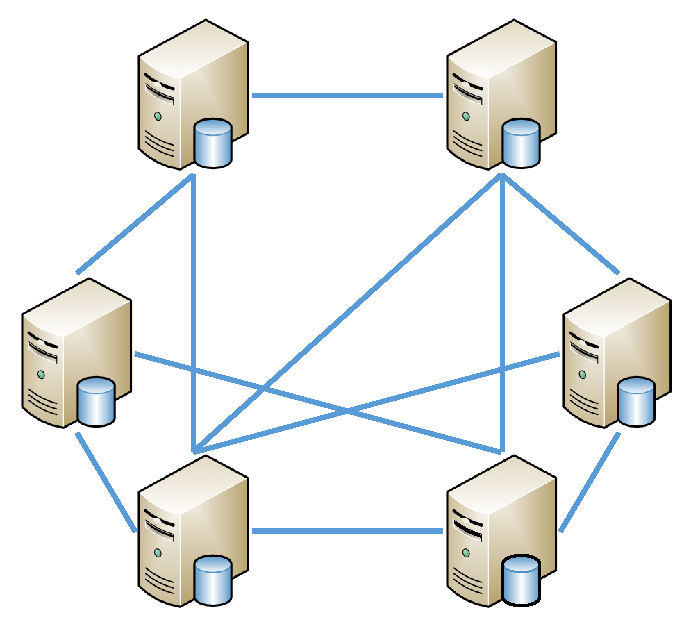
\includegraphics[width=1.78in]{Fig/chapter1/p2p.eps}
         	}
         	\subfigure[主从式]{
         		\label{fig:MS}
         		
         		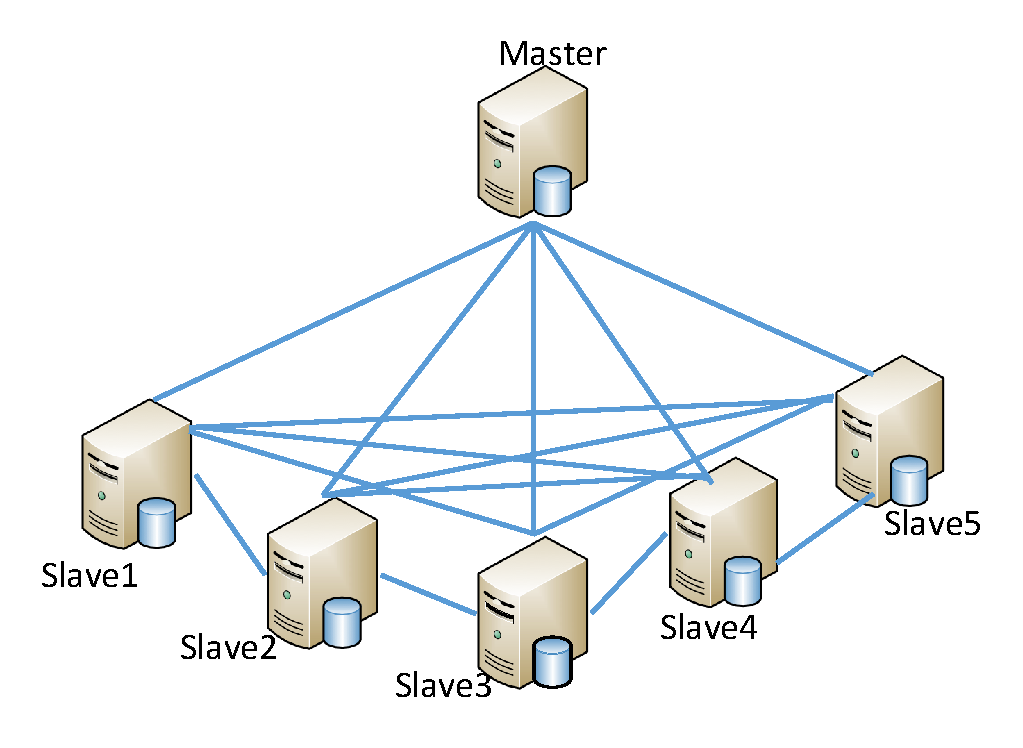
\includegraphics[width=1.78in]{Fig/chapter1/MasterSlave.eps}
         	}
         	\subfigure[协调者-远程结点式]{
         		\label{fig:CR}
         		
         		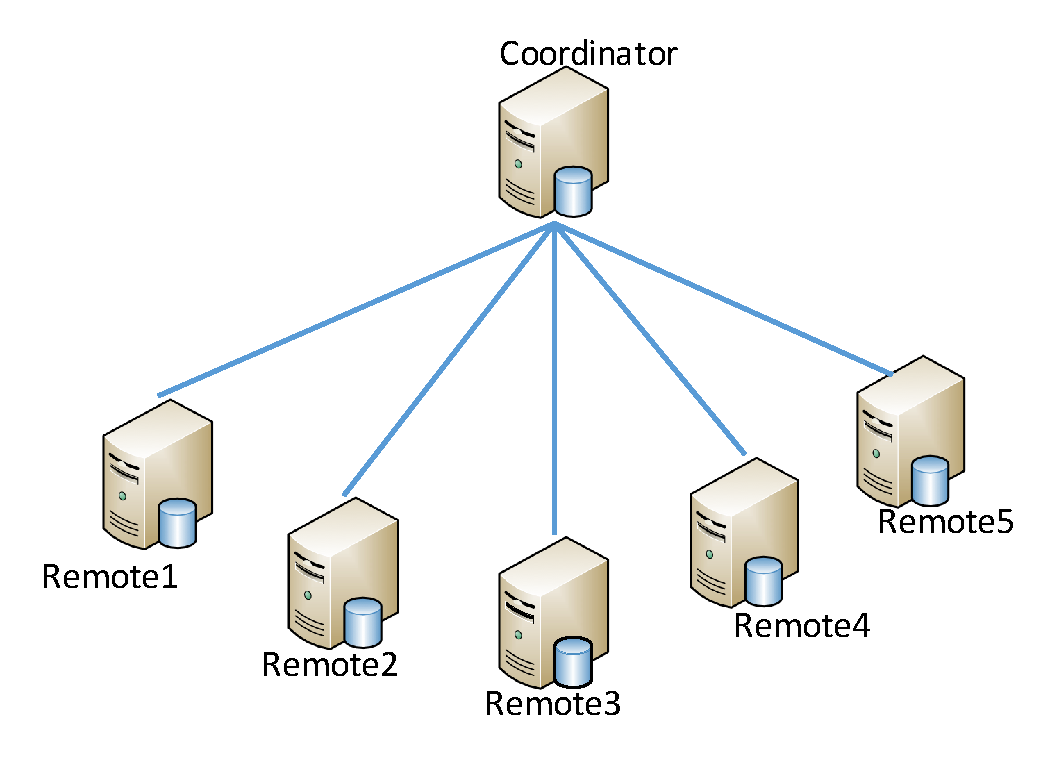
\includegraphics[width=1.78in]{Fig/chapter1/CoorRemote.eps}
         	}
         	\caption{3种常见分布式架构}
         	\label{fig:DistributeArc}
         \end{figure}
         
         此外,轨迹数据由于来源广、数据量大等特性,往往以分布式形式采集和存储在各结点中。这类结点既可以是管理着大量轨迹数据的高性能服务器也可以是管理单一移动对象的的个人智能手机。此外,结点间可能相互独立,不能互相访问。因此,
         如何对分布在具有不同存储和计算能力的各个结点上的分布式轨迹数据进行统一的管理、分析和挖掘服务是合理利用迹数据的首要问题。现有的分布式解决方案可分为以下三类:(i)基于对等系统(Peer-To-Peer,P2P)架构的处理方案。该架构中各个结点能互相访问且各个结点都有原始数据的完整备份,因此不适用与轨迹大数据。
         (ii)基于主-从式(Master-Slave)的分布式集群架构的处理方案。该架构中由一个主(Master)结点和多个从(Slave)结点构成,其中从结点存放具体数据并负责任务的执行,主结点存放数据的元数据并负责任务的分发和调度。基于该类架构典型的处理系统有Hadoop和Spark。该架构往往要求所有物理结点在同一个集群内部,结点间通过高速网络连通。
         (iii)基于协调者-远程结点的(Coordinator-Remote Site)的分布式架构。该架构中存在一个协调者和多个远程节点,其中协调者结点不存储任何数据只负责跟远程结点通信,而远程结点负责存放本地数据,且各远程结点间互不通信。 
         第三种方案可看做第二种方案的推广,首先它允许所有结点物理上互相远离,不要求它们位于同一集群内部。其次,远程结点间做到完全独立且互不知晓。最后,协调者结点不需要知道远程结点数据的任何信息。
         以上三点能有效地保证数据拥有者的隐私和数据存储、计算的独立性。因而,本文研究的分布式场景选择第三种处理框架。
   %      第一种架构要求数据共享,这不符合目前轨迹数据源间相互独立互不共享的特性。第二种架构要求数据集中在同一个物理集群中,而现实的轨迹数据存放在物理上相互远离互不知晓的节点中。第三种架构中,协调者节点用于接受用户的查询请求,各远程节点各自保存本地数据且互不知晓,远程节点仅与调节着结点进行通信。
  %    因此,前两个架构均不符合轨迹大数据的实际存储状况,仅第三种架构符合我们的需求。  
  
  目前,分布式轨迹相似度研究已经得到广泛的重视。文献\cite{setSimilar,kimICDE2012}研究了主-从式架构下轨迹数据的join查询,其关注重点是如何降低从节点间数据交换量过高的问题。文献\cite{KDDSimilarity} 研究了基于协调者-远程节点架构下的$k$近邻轨迹查询研究。其研究的是用户手机连接基站的轨迹数据并将每个基站看做一个远程节点。由于手机在用户移动过程中会连接到不同的基站,故轨迹数据被切割成若干数据片段存放在不同的基站中。在该研究中,其研究目标是如何提高查询的效率而未关注如何降低通信开销。类似的,
Smart Trace\cite{SmartTrace} 和 Smart Trace$^{+}$ \cite{crowdsourced} 在相同的系统架构中研究了相同的问题,但在其研究内容中,将每个智能手机看做远程结点且每个结点仅保存一条轨迹数据。在这两项工作中,计算效率和通信开销同时得到了考虑。与以上不同的是,本文研究了更加抽象的分布式场景,即每条轨迹完整的保存在一台远程结点上,且每个远程结点可存储多条轨迹数据。
此外,文献\cite{trajectoryVLDB}提出了基于Spark的$k$近邻轨迹查询系统。该系统由于不满足应用中远程结点间相互独立、互不知晓的要求,因而无法推广到本文所提查询中。
  
  		                                                                                              

\section{研究内容与挑战}\label{sec-c1-content}
\begin{figure}
	\centering
	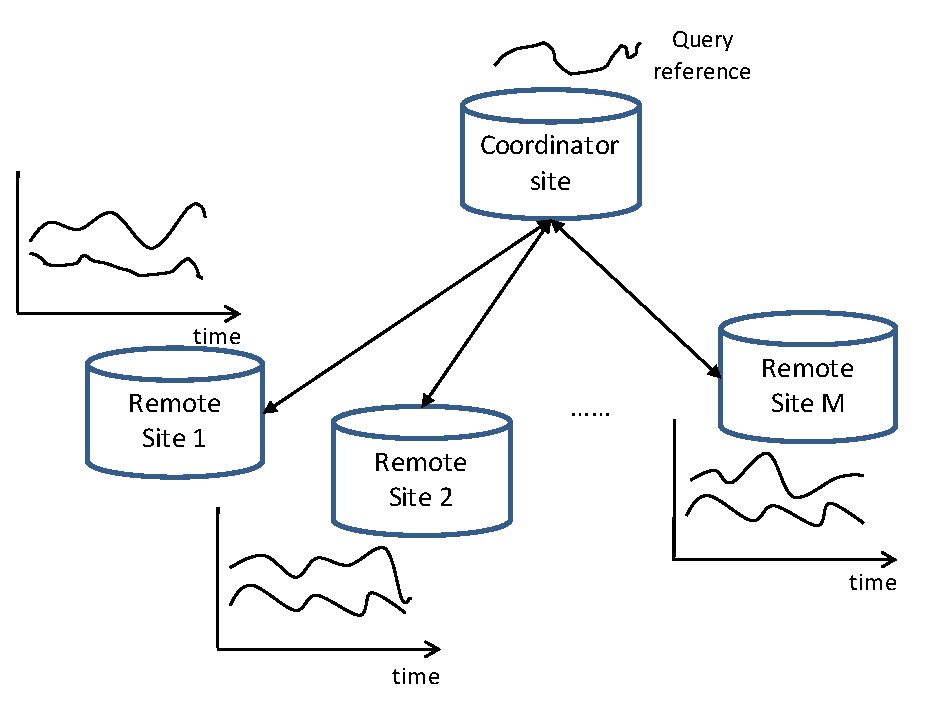
\includegraphics[width=0.73\textwidth]{Fig/chapter1/coor-remote}
	\caption{查询展示}
	\label{fig-chapter1-demonstrate}
\end{figure}

本文选用基于协调者-远程节点的分布式架构进行管理和分析轨迹大数据,并对轨迹大数据上的$k$近邻轨迹查询进行了研究。该系统架构中存在一个协调者结点和$M$个远程结点。协调者节点和所有远程结点连通,但不知道远程结点的数据信息。远程结点间彼此独立且互不通信。在实现查询过程中,协调者结点扮演查询引擎的角色,其接受用户提交的查询,并将查询相关数据发送给远程结点。每个远程结点根据接收到的数据返回响应的查询结果。
基于此框架,本文所研究查询如图\ref{fig-chapter1-demonstrate}所示。协调者节点负责接收用户提交的查询轨迹,每个远程结点存储一部分轨迹数据。协调者节点的目标是从所有远程结点中找出与查询对象最相似的$k$条轨迹。
一个直观的解决方案就是用户将$\cal Q$提交给协调者结点后,该结点直接将$\cal Q$发送给所有的远程结点。远程结点接收到查询对象后,计算其与本地存储的所有轨迹间的距离并将相似度值返回给协调者结点。最终,协调者结点从接收到的距离值中选择最小的$k$个作为结果返回给用户。这样的解决方案,设计简单且易于实现,但也存在着通信量过大的问题,尤其是当待查询轨迹数据量较大或远程结点较多时。因此,如何降低通信开销是我们需要解决的首要问题。此外,该方案中由于需要对查询轨迹和远程结点间的轨迹进行距离值计算,导致其
计算开销也较大,我们需要考虑如何提高查询的执行效率。
最后,如上节所介绍,轨迹间的距离计算准则很多,现有工作只针对某一具体距离来进行通信或效率优化。因而,缺乏统一的框架或方法来处理。综上所述,
本文研究面临的挑战主要表现为以下3点:
\begin{itemize}
	\item  \textbf{首先,针对时间序列上已有的$k$近邻轨迹查询技术往往只针对某一距离准则设计,缺乏通用性。}距离度量选择准则是轨迹数据挖掘分析的核心内容之一,选用不同的度量函数,导致的挖掘结果以及对结果的理解往往大不相同。现有的工作都是针对某一研究问题,精心挑选或自定义一距离函数以满足研究的需要。因此,所提出的解决方案具有较高的局限性,很难推广到其他的问题中。为此,需要提出通用或对一类问题适用的解决方案。
	
	\item \textbf{其次,现有分布式$k$近邻查询算法中仍然存在着通信开销过大的问题。}直接将原始查询轨迹发送到所有远程结点的方式,其通信开销随轨迹长度和远程结点的个数的增加而快速增大。而现有的数据降维方案如Douglas-Peuker算法、奇异值分解(Singular Value Decomposition, SVD)、离散傅里叶变换(Discrete Fourier Transform, DFT)、哈尔小波变换(Haaar Wavelet Transform, HWT)、分段聚合近似(Piecewise Aggregate Approximation, PAA)、自适应分段常量近似(Adaptive Piecewise Constant Approximation, APCA)等方法虽然降低了数据的维度,但也造成了数据信息损失,使得数据不再直观且不能保证结果的准确性。此外,这些方法常用于处理一维时间序列数据,而轨迹是天然的多维时间序列数据。为此,需要提出新的轨迹数据降维方法,在保证查询结果正确性的同时,降低通信开销。

	\item \textbf{最后,现有的分布式top-$k$查询时间效率需要得到提升。}轨迹距离的计算除欧式距离是一次的计算复杂度,其他往往需要二次的计算复杂度。在每个远程结点进行查询轨迹与局部保存的轨迹进行两两相似度计算的方案不可行。虽然适用传统索引技术是加快查询速度有效工具,但索引技术只能针对原始轨迹数据,无法适用于降维后的数据。为此,需要设计新的方案来提高查询效率。
	
\end{itemize}

\section{主要贡献}\label{sec-c1-contribution}
本文围绕分布式$k$近邻轨迹查询这一问题,系统性的提出了解决方案。首先,针对轨迹距离度量的多样性,提出了两种查询实现框架以覆盖所有的距离函数。这两个框架分别针对不同类别的距离度量准则,在保证查询结果正确性的同时能有效地降低通信开销。接着,我们将两个常用相似度距离函数分别嵌入到两个框架中,并提出了对应的算法。最后,使用真实轨迹数据集验证了算法的性能。因此,本文的主要贡献分为以下3点:
\begin{itemize}
	\item  \textbf{针对通信开销较高问题,提出了两个通用查询实现框架FTB(Framework with Two Bounds)和FLB(Framework with Lower Bound)。}FTB框架中要求能根据降维后的概要数据计算出相似度距离的上下界,并能保证概当细粒度的概要数据获取后,所计算出来的上下界越来越紧并最终能收敛。FLB框架中仅要求能根据降维后的概要数据计算出相似度距离的下界,且能保证当细粒度的概要数据获取后,所计算出来的下界越来越紧。这两个框架由于仅需要传递查询轨迹的概要数据,因此能大大降低通信开销。
	
	\item \textbf{针对FTB框架,提出了基于欧式距离的FTB-ED 算法。}为验证FTB框架的有效性,本文研究了如何将具体欧式距离嵌入到该框架中。为此,本文首先利用Haar小波变换以得到不同粒度的轨迹概要数据,并证明了全部概要数据的欧式距离等于原始轨迹数据的欧式距离。接着,利用部分概要数据,本文提出了基于欧式距离的轨迹相似度上、下界,并理论证明了该相似度的正确性。然后,我们将该上、下界应用到FTB框架中,提出了FTB-ED算法。在该算法中,我们引入了性能优化策略以提高查询效率。
	最后,我们通过大量实验验证了FTB-ED算法的有效性和可扩展性。
	
	\item  \textbf{针对FLB框架,提出了基于动态时间卷曲距离的FLB-DTW算法。}为验证FLB框架的有效性,本文研究了如何将具体动态时间卷曲距离嵌入到该框架中。
	为此,本文首先针对查询轨迹使用不同粒度的包围信封(Bounding Envelope)来表示轨迹的概要数据。接着提出了基于动态时间卷曲距离的下界,并理论证明了该下界的正确性。最后将该下界应用到FLB-DTW框架中,并提出了FLB-DTW算法。在该算法中我们引入了多种机制以提高查询效率。最后,我们通过大量实验验证了FLB-DTW算法的有效性和可扩展性。
	
\end{itemize}



\section{章节安排}
\begin{figure}
	\centering
	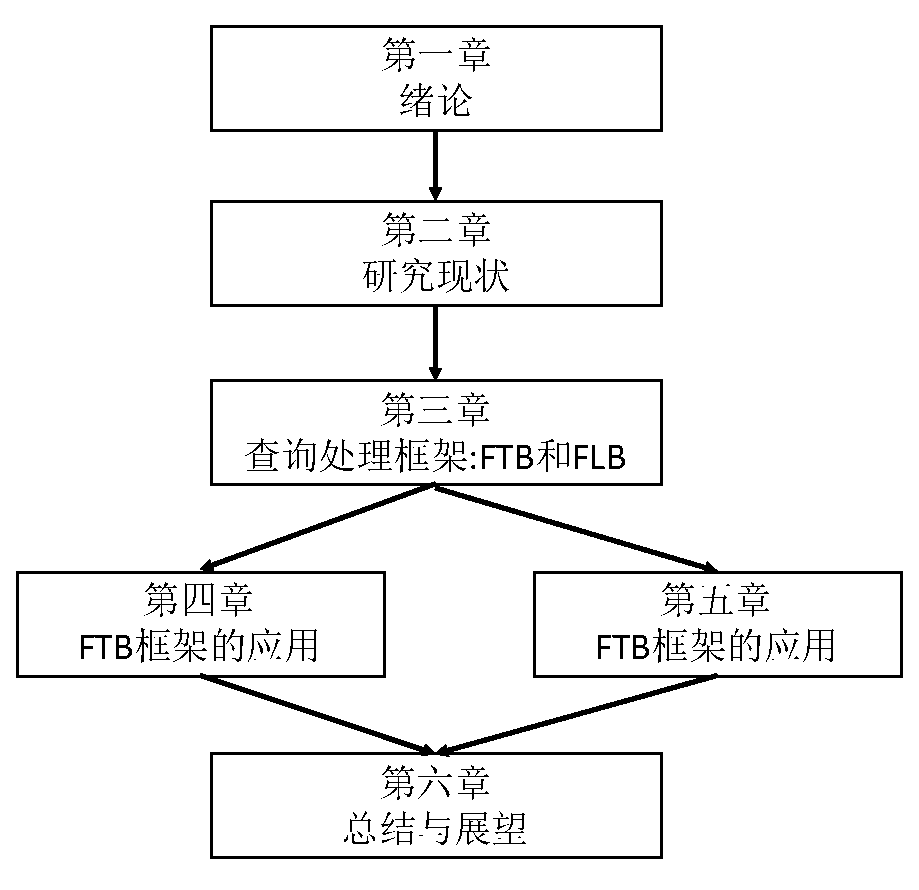
\includegraphics[width=0.63\textwidth]{Fig/chapter1/paperStructure}
	\caption{本文的组织结构}
	\label{fig-chapter1-structure}
\end{figure}
本文一共分为六章,章节安排如图~\ref{fig-chapter1-structure}所示:
\begin{itemize}
	\item 第二章从轨迹数据存储、轨迹降维以及轨迹数据相似性查询三个方面介绍了研究背景知识和研究现状。
	\item 第三章介绍了两个通用查询处理框架FTB和FLB以分别处理能同时提供上、下界的和仅能提供下界的距离准则。
	\item 第四章介绍了如何将欧式距离嵌入到FTB框架中,并提供高效的查询结果。
	\item 第五章介绍了如何将DTW距离嵌入到FLB框架中,并提供高效的查询结果。
	\item 第六章对上述已有工作进行了总结,并展望了未来的研究方向和内容。
\end{itemize}

\clearpage
\phantom{s}
\clearpage  %%%%%%%%%%!!!!!!!!%%%%%%%
\chapter{问题定义及研究现状}\label{chapter:relatedwork}
本章第一节首先对数据模型和要解决的查询问题进行了定义,然后从以下方面介绍了相关的研究工作:轨迹索引、轨迹降维、轨迹相似度度量、时间序列数据top-$k$查询,最后对本章内容进行小结。

\section{问题定义}\label{chapter-related-coll}
本文的研究目标是给定一条查询轨迹,从存储在若干远程结点中的轨迹中找出$k$条距离最短或相似度最高的轨迹。为此,本节首先介绍了轨迹数据模型,接着介绍了查询的定义。

\subsection{轨迹数据}
轨迹是描述移动对象移动行为的数据。通常来说,一条轨迹$T$可看做包含$n$个元素(即轨迹点)的有序序列。每个轨迹点$\vp$包含了时间、位置等维度的信息。因此轨迹可被形式化定义为如下:
\begin{define}[轨迹]
轨迹形式化表示为:$T=\{\bp_{0}, \bp_{1},\cdots, \bp_{n-1}\}$。
\begin{equation}
T=\{\bp_{0}, \bp_{1},\cdots, \bp_{n-1}\}
\end{equation}
其中$|T|=n$代表轨迹所包含的点数,即轨迹的长度。每个轨迹点$\bp$包含时间($t$)、位置($l$)等维度的信息。因而$|\bp|=d$称为轨迹的维度。此外轨迹中的点严格按时间升序排列,即$\forall i,j,0\le i\le j < n$则$\bp_{i}.t \le \bp_{j}.t$。
\end{define}

轨迹数据的来源多样且复杂。根据移动对象的划分可分为如下几类:
\begin{itemize}
	\item \textsf{人类活动轨迹数据:}该类数据分为主动式和被动式。主动式数据是人们主动利用移动定位设备分享或汇报自己的位置等信息。典型的有社交网络中的数据,用户提交位置获得服务的数据。被动式数据是人们无意间使用各种服务时所产生的轨迹数据。典型的有公交刷卡轨迹和手机的信令轨迹数据。

	\item \textsf{交通工具轨迹数据:}这类数据主要是交通工具使用车载GPS设备所产生的移动轨迹数据。例如,出租车、公交车的活动轨迹数据。
	
	\item \textsf{动物活动轨迹数据:}这类数据是为了研究动物生活、迁徙等行为和习惯而捕获的数据。
	
		\item \textsf{自然现象活动轨迹数据:}这类数据典型的有台风、冰山、海洋事件等的轨迹数据,用以探索自然现象的活动规律。
\end{itemize}

轨迹数据符合大数据时代的 3V 特征,即量大、实时、多样。轨迹数据采样由于受设备、采样频率等因素影响,数据质量较低且各个轨迹的采样间隔差异显著。
这些问题导致原始轨迹数据的可用性较低。因此,我们在进行轨迹数据分析前往往需要经过数据清理(data cleaning)、地图匹配(map mathching)、轨迹分段(trajectory segmentation)等预处理方式化为校准轨迹。校准轨迹数据能够通过数据管理技术进行轨迹索引以便有效地存取。因此,本文所处理的轨迹数据为预处理后的校准轨迹数据。这样的数据有如下特点:(i)采样频率一致;(ii)长度一致;(iii)位置精度高。
这为我们挖掘轨迹模式从而提炼有价值的知识提供了可靠保障。

\subsection{分布式$k$近邻轨迹查询}
轨迹数据往往是分布式采集并存储的。为此假设有$M$个远程结点,每个远程结点$i$包含轨迹数据集${\cal D}_{i}$。那么整个分布式轨迹数据集${\cal D}=\bigcup_{i=1}^{M} {\cal D}_{i}$。我们的目标是给定查询轨迹,从分布式存储的${\cal D}$数据集中,找出与其距离最近的$k$条轨迹。下面我们将给出查询的形式化定义:
\begin{define}[分布式k近邻轨迹查询]
	该查询形式为query$({\cal Q}, {\cal D},DM,k)$,其中$\cal Q$为给定查询轨迹,${\cal D}$为分布式轨迹数据集, $DM$为距离度量准则以及$k$为返回结果集大小。查询的目标是返回满足如下条件的轨迹集$\cal S$:(1)${\cal S} \subseteq {\cal D}$;(2)$| {\cal S}|=k$;
	(3)$\forall {\cal C} \in {\cal S}, {\cal C}' \in {{\cal D} - \cal S}$,$DM({\cal Q},{\cal C}) \le DM({\cal Q},{\cal C}')$。
\end{define}


传统的集中式环境下$k$近邻轨迹查询相比,分布式场景下的查询不仅注重查询效率,而且尤其注重通信开销。这是由于分布式场景中,远程结点和协调者结点的带宽资源往往是有限的。高的通信开销,意味着用户可能要花费更多的金钱。因此,用户允许多花一点时间以达到降低通信开销的目的。

\section{轨迹压缩}\label{sec-c2-reduction}
将查询轨迹数据压缩是降低通信开销的有效方式。如图\ref{fig-chapter2-compress}所示,现有轨迹压缩的方法根据处理数据类型的不同可分为3类\cite{jiang}:第一类是传统的时间序列压缩算法,其根据应用场景又可以分为离线和在线压缩两类算法。第二类是基于路网结构的轨迹压缩算法,该类算法依赖于所给路网数据。第三类是语义压缩,其目标是将原始数值型轨迹数据转换为人们能理解的语义信息。
\begin{figure}[t]
	\centering
	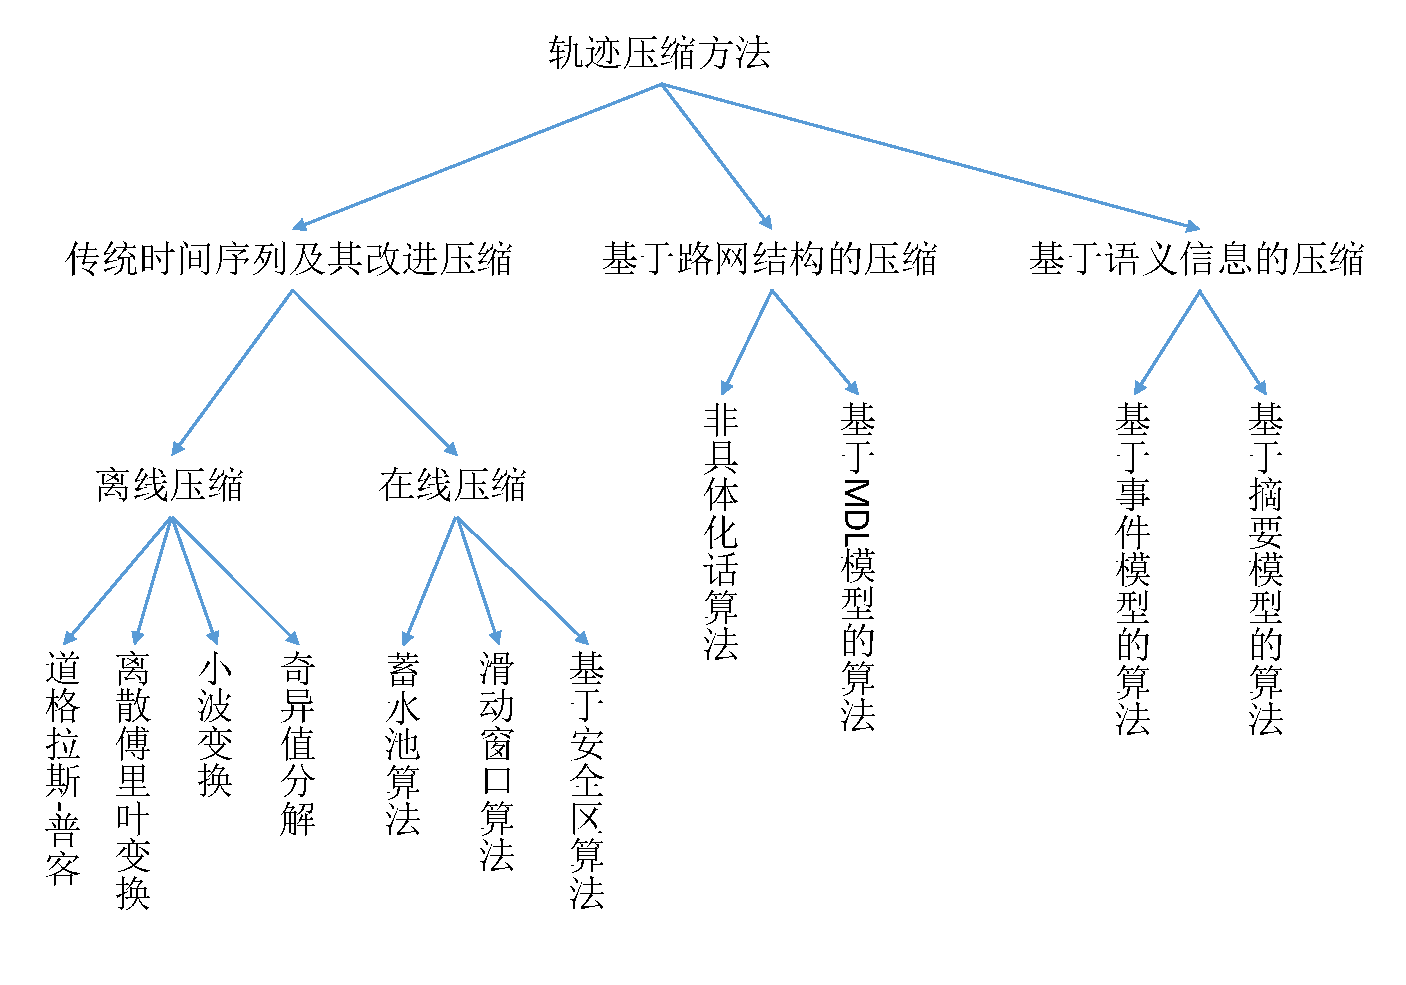
\includegraphics[width=0.73\textwidth]{Fig/chapter2/Compress}
	\caption{基于安全区的压缩算法}
	\label{fig-chapter2-compress}
\end{figure}
\text{常用轨迹压缩算法}

\subsection{传统离线时间序列压缩算法}
离线轨迹压缩算法主要的应用场景是,给定一静态历史轨迹数据库,对其中的轨迹进行压缩。该类压缩算法不考虑数据集的增加、删除和修改。
该类算法的提出主要是为了解决时间序列数据的降维(降低序列的长度)。由于轨迹本质上也是时间序列数据,因此该类方法也可用于轨迹的压缩。这是由于轨迹数据的各属性维度上数据一般互相独立,因此只需将降维方法应用到各个维度上分别进行压缩即可。本节主要介绍几种典型的离线时间序列(含轨迹)压缩算法。


%但是,和一般的时间序列不同,轨迹数据又有其特别之处,比如其包含了物体的运动方向、速度等。因此,也有些轨迹压缩算法将这些性质特征考虑在内,设计了专门用于轨迹数据的压缩算法。

\textbf{道格拉斯-普克算法:}
道格拉斯-普克(Douglas-Peucker, DP) 算法将原始时间序列看作一条多维曲线,其目标是找出一条与原始曲线相似但使用更少点构成的简化曲线。此外,构成简化曲线的点必须来自原来曲线。
该算法中原始轨迹与简化轨迹间的“不相似性”是通过两条曲线间的豪斯多夫(Hausdorff)距离表示。简化曲线中的点即为压缩后的数据。
道格拉斯-普克算法的过程由如下5个步骤构成:(1)在曲线首尾两点A,B之间连接一条直线AB;(2)找出曲线上离该直线段距离最大的点C,计算其与AB的距离;(3)比较该距离与预先给定的阈值的大小,如果小于阈值,则该直线段作为曲线的近似,该段曲线处理完毕;(4)如果距离大于阈值,则用C将曲线分为两段AC和BC,并分别对两段取信进行1至3步的处理;(5)当所有曲线都处理完毕时,保留依次收集分割点,得到压缩后的点集。DP算法的思想简单且性能较好,在各个领域都有广泛的应用。但其缺点就是算法复杂度较高达到$O(n^2)$,$n$是轨迹长度。文献\cite{DPSpeeding}提出了借助外部存储结构的改进算法,把时间复杂度降低为$O(n\log n)$。此外,文献\cite{MeratniaB04}和\cite{LiuZSSKJ15}分别提出了同时时间和空间维度的改进距离函数( Time-Distance Ratio, TDR)和(Top-Down Time Ratio, TD-TR),克服了DP仅考虑空间维度的缺点。

\textbf{离散傅里叶变换:}
离散傅里叶变换(Discrete Fourier Transform, DFT)\cite{DFT}是时间序列数据降维的常用方法,并且已有许多扩展和改进方案被提出\cite{fastDFT,rafiei1997similarity,rafiei1999on}。
其基本思想是任何一个信号,不管其多复杂,都可以分解为有限个正弦和余弦曲线的叠加。每条曲线可以由一称为傅里叶系数的复数表示\cite{Shatkay1995The}。此时,我们时间序列由时域变换到频域了。使用频域的好处有很多,其最重要的就是能进行数据压缩。一条长度为$n$的信号(即时间序列)可以被分解为$n$个正/余弦曲线,且这$n$个曲线能重新组合成原来的信号序列。但由于$n$个曲线中存在着许多振幅较低的,这些低振幅曲线对重新构建原来的信号的贡献较低。因此,其对应的低振幅系数可以被丢弃掉,而保留那些振幅较高的系数。这些保留的系数重新组合所构成的信号数据与原始信号数据相比,并没有太多的信息丢失。因而,达到了使用少量数据来表示原始信息的目的。

此外,文献\cite{Shatkay1995The}中提出原始时域内信号数据间的欧式距离等于变换后频域内系数间的欧式距离。这一结果称为帕斯瓦尔定理(Parseval's law)。因此,若经离散傅里叶变换且将低振幅的系数丢掉后,使用剩下的系数计算距离,所得到的结果必然是原始欧式距离的下界(丢失的数据都是正数)。文献 \cite{KeoghDimReduction}提出了基于该下界的剪枝方法。

\begin{figure} [t]
	\centering
	\subfigure[压缩前后数据]{
		\label{fig:comp}
		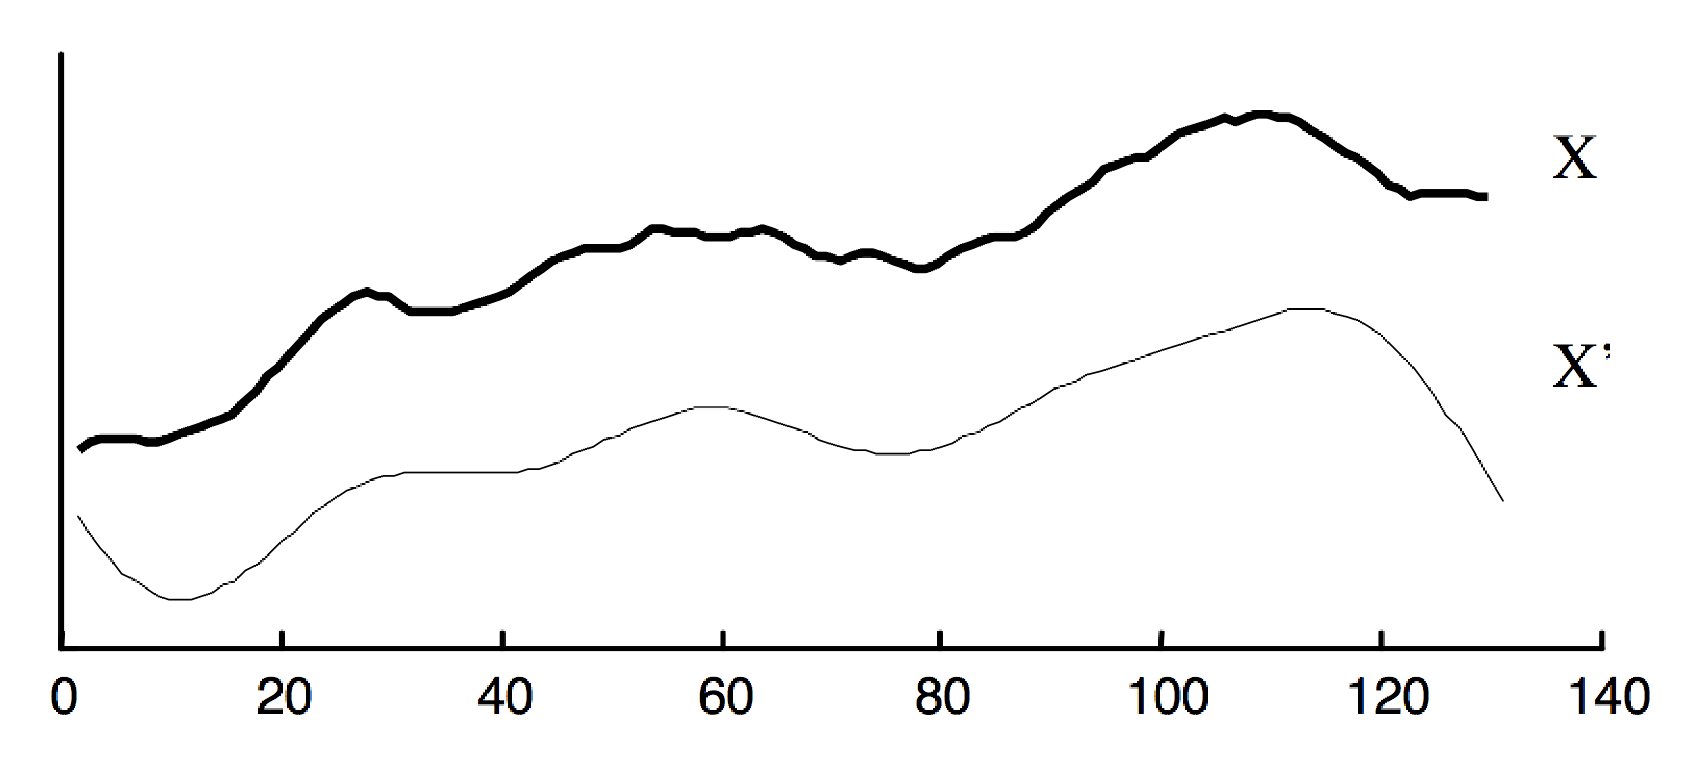
\includegraphics[width=0.45\textwidth]{Fig/chapter2/signal.eps}		
	}
	\subfigure[DFT系数]{
		\label{fig:coefficietns}
		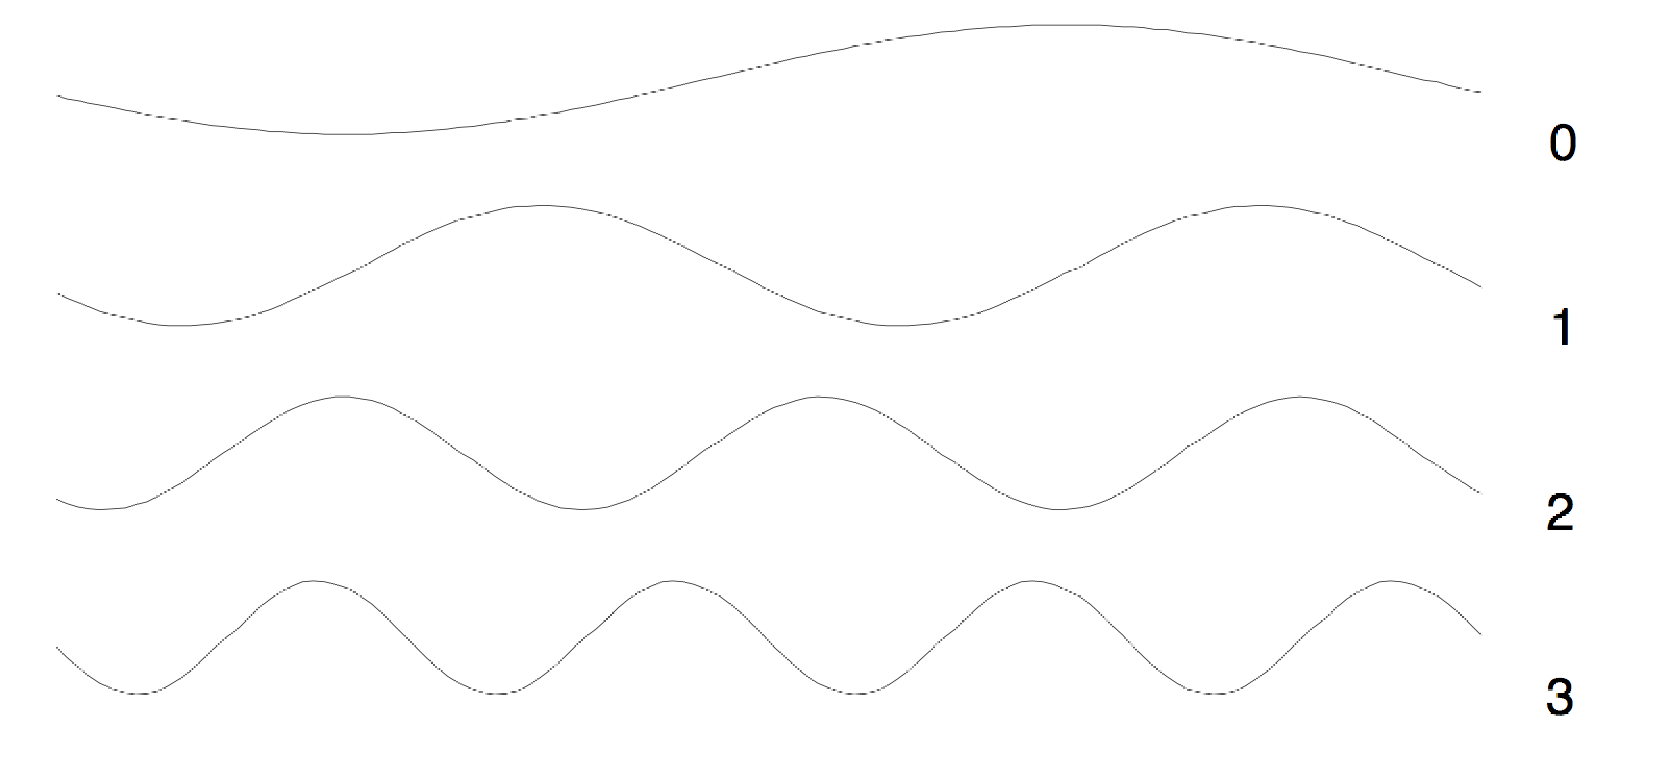
\includegraphics[width=0.45\textwidth]{Fig/chapter2/DFT.eps}
	}
	\caption{离散傅里叶压缩数据\cite{KeoghDimReduction}}
	\label{fig-chapter2-DFT}
\end{figure}

为将以长度为$n$的时间序列降低到$N$维特征。我们调用离散傅里叶变换并保留了$N/2$个系数。保留$N/2$而不是$N$的原因是每个系数是一个复数,我们需要同时保留实部和虚部的值。图\ref{fig-chapter2-DFT}介绍了使用离散傅里叶变换进行压缩数据的思想。首先对左图原始信号$X$进行傅里叶变换。然后只保留了如右图振幅较高的4个曲线。接着,我们利用保留的4个系数恢复出原始轨迹的近似轨迹$X'$。在我们的分布式查询中,可以通过发送压缩后的 系数数据以达到降低通信开销的目的。

\textbf{小波变换:}
小波变换(Wavelet Transform) 将信号分解为一系列基/母小波函数的和与差的组合,这一点与离散傅里叶变换类似。但它们之间也有许多的不同点。其中一个重要的区别是,小波在时间上是局部的,即小波系数只代表原始数据中的一小部分子段。这也是“小波”这一名词的由来,“小波”就是小区域、长度有限、均值为0的波形。
而傅 里叶系数总是代表着数据的全局信息。对于一些需要研究数据局部信息的应用来说,具有多解析度特性的小波变换更为适用。

\begin{figure} [t]
	\centering
	\subfigure[压缩前后数据]{
		\label{fig:haar}
		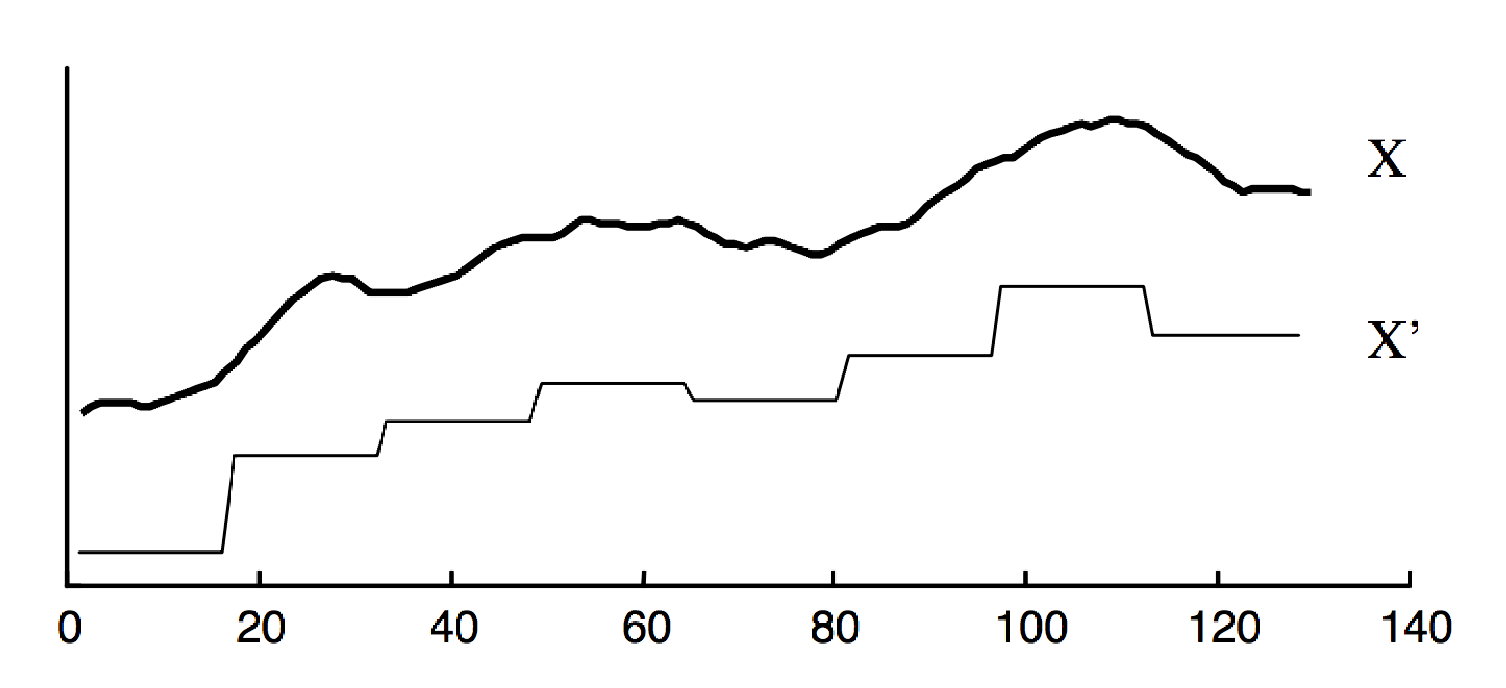
\includegraphics[width=0.45\textwidth]{Fig/chapter2/Haar.eps}		
	}
	\subfigure[DFT系数]{
		\label{fig:haarcoeff}
		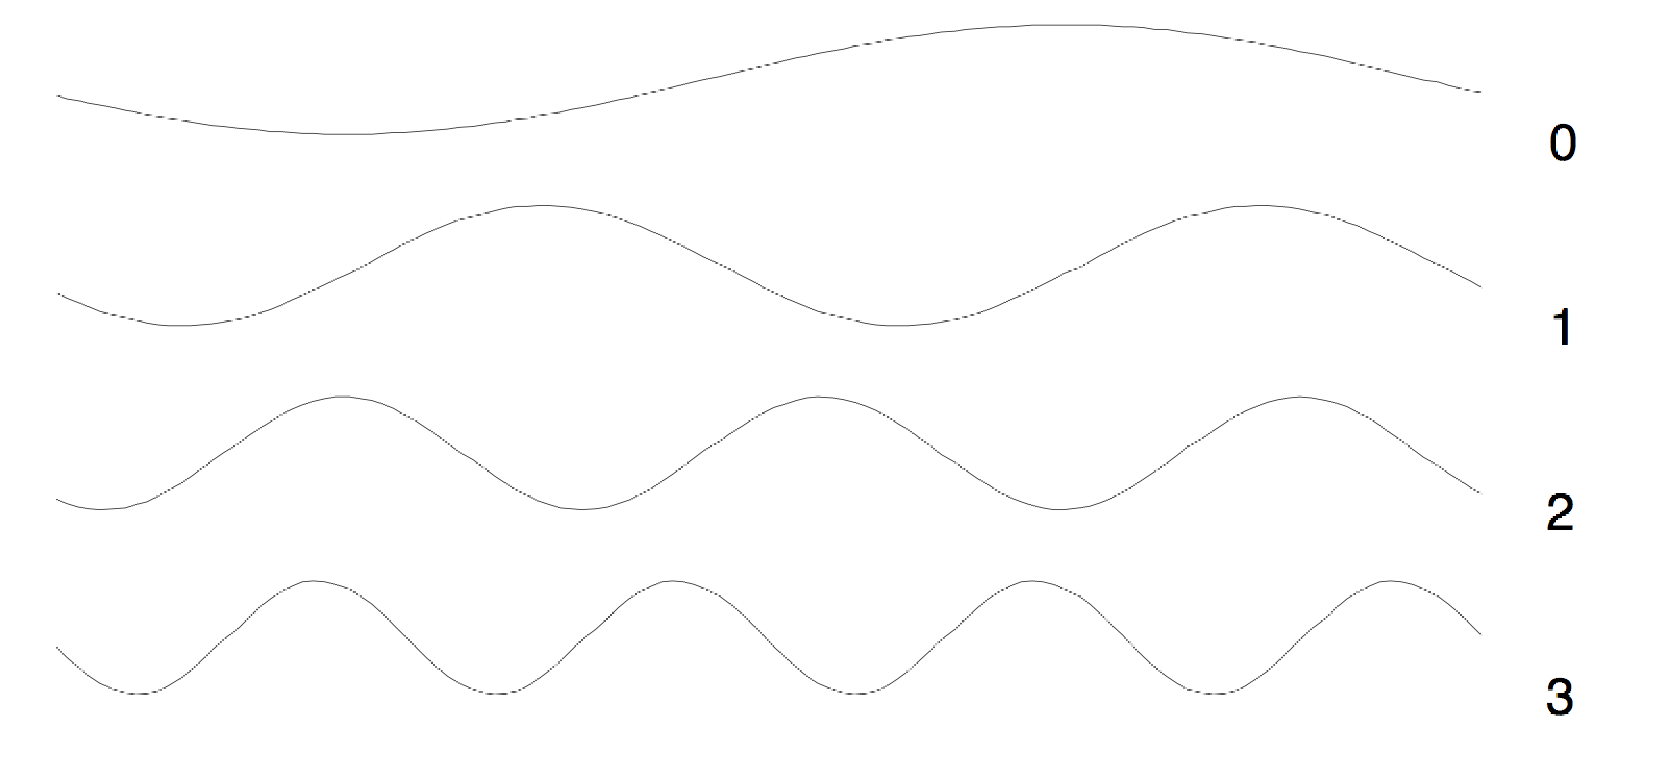
\includegraphics[width=0.45\textwidth]{Fig/chapter2/DFT.eps}
	}
	\caption{哈尔小波压缩数据\cite{KeoghDimReduction}}
	\label{fig-chapter2-haar}
\end{figure}
当原始信号/时间序列数据被小波分解之后,会得到一个小波系数序列。该序列的前几个系数包含了数据的总体信息,是对原始信号数据的粗粒度估计。
而其余的系数则包含着数据局部的细节信息。因此使用 小波变换压缩数据,就是通过只保留前几个系数,以大体上逼近 原始的数据,达到降维的目的。其代价是损失一些局部的细节信息。这一点跟傅里叶变换进行压缩一样,两者都是有损压缩。近年来,小波变换由于其同时保持了时域和频域的特征(傅里叶只包含了频域特性),在数据压缩、过滤、分析等领域得到广泛应用。

哈尔小波是表达和计算都最简单的一种小波。它的基函数是均值和差值函数。
Chan等人证明了原始时域内信号数据间的欧式距离等于变换后哈尔小波系数间的欧式距离\cite{chan2003haar}。
图\ref{fig-chapter2-haar}展示了经过哈尔小波变换压缩数据的过程。对于给定的时间序列$X$,经过哈尔小波变换后,我们只保留了右图所示前8个系数。利用这8个系数,我们可以计算出原始时间序列的近似值$X'$。在我们的分布式查询中,可以通过发送这些前面的哈尔小波系数以达到降低通信开销的目的。

\textbf{奇异值分解:}
尽管奇异值分解(Singular Value Decomposition, SVD)方法已经成功应用于图像和多媒体数据的分析中。现有的大量工作表面,其也可以被应用于时间序列数据的索引和压缩中。

前面介绍的几种方法都是对单一轨迹进行压缩,各个轨迹之间相互独立。奇异值分部街不是针对单个时间序列对象进行压缩,而是对全局数据进行整体变换,以得到整体数据的压缩结果。
其分解过程如下,首先将整个数据集进行变换,在原始的数据空间中顺序地找一组相互正交的坐标轴,其中沿第一个坐标轴方向的方差最大,而在与第一个坐标 轴正交的平面上,沿第二个坐标轴方向的方差最大,在于第一个坐标轴以及第 二个坐标轴正交的平面中,沿第三个坐标轴的方向方差最大,依次类推。对于长度为$n$的时间序列,可以通过奇异值分解找到$n$个满足条件的坐标轴。为了达到降维的目的,
取前$N$个坐标轴构成一个$N$维的空间来近似原来的$n$维空间,这样就将一个$n$维空间变换成了$N$维的近似空间,且使用上述方法选择 的$N$个坐标轴所张成的空间中,数据的损失最小。

\subsection{传统在线时间序列压缩算法}
离线的轨迹压缩算法可以充分根据轨迹的所有信息来获取较好的压缩效果。但对于实时在线场景,我们无法事先得到完整的轨迹数据,因而需要在线算法来进行实时压缩。相比于离线压缩算法,降低计算开销是在线算法的重要内容,它需要快速确定是否要保留刚刚到来的轨迹点。为此,我们将介绍几种典型的在线算法。

\textbf{蓄水池算法:}
蓄水池算法(Reservior Sampling Algorithm)\cite{Reservoir}的思想是为每个时间序列维持一个大小为$R$的缓冲区,并用这$R$个点来近似原始轨迹。由于轨迹数据是持续增加的,无法知道轨迹的最终长度。因而,该算法所要解决的核心问题就是无放回替换,即当一个点从缓冲区删除掉后,不能再将它取回。它的做法是,首先将前$R$个轨迹点放入缓冲区,当新的轨迹点到来时,判断该点是否需要放入缓冲区。具体地,当第$k$个点到来时($k>R$),该算法以$R/k$的概率判断改点是否需要加入缓冲区。如果判断结果正确,则从现有的轨迹点中随机删除一个点,并将新点加入。该算法的时间复杂度为$O(R(1+\log N/R))$,因此效率较高。但它没有考虑轨迹的时间或空间属性,因而近似轨迹无法保留轨迹的原始特征。

\textbf{滑动窗口算法:}
与蓄水池算法不同的是,滑动窗口算法\cite{ICDMSiding,EDBTSliding}的思想是维护一个不断增大的缓冲区,并用缓冲区中的轨迹来近似原始轨迹。它的算法过程是,首先选取第一个点作为锚点,用$\vp_a$来标识,然后将下一个点加入滑动窗口中。当新点$vp_{i}$加入后使用$\overline{\vp_a \vp_i}$来拟合窗口中所有点组成的字轨迹。若$\overline{\vp_a \vp_i}$拟合误差小于给定的阈值,则继续加入新点。否则,将$\vp_a$与$vp_{i-1}$之间的点从缓冲区删除,并使用$vp_{i-1}$作为新的锚点。该算法能有效保留轨迹的原始时空特征。

\begin{figure}
	\centering
	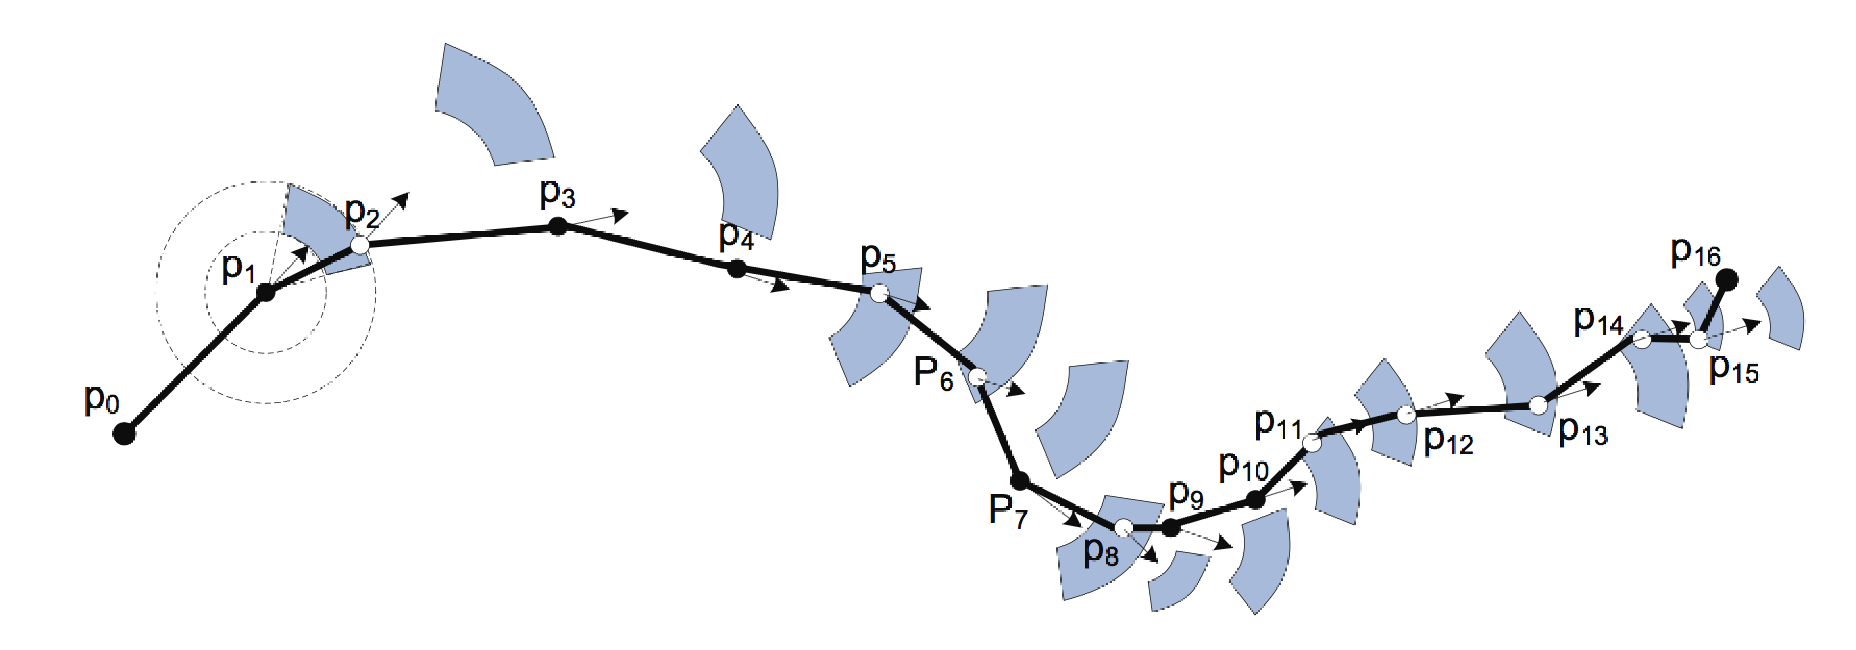
\includegraphics[width=0.73\textwidth]{Fig/chapter2/safearea}
	\caption{基于安全区的压缩算法\cite{Zheng2011Computing}}
	\label{fig-chapter2-safeare}
\end{figure}
\text{基于安全区的算法:}
以上压缩算法没有考虑轨迹中所蕴含的速度和方向等特征,为此Potamias\cite{SSDBMSample}等认为,一个轨迹点只要能表示轨迹发生了改变,就应该包含到最终的压缩轨迹中。而如果一个点可以从之前的运动中通过插值或位置预测等方法计算出来,那么就可以将其舍弃。因此,他们认为在轨迹压缩过程中应该考虑速度和方向这些特征,因为这些可以用来预测轨迹的位置。
因而中提出了一种阈值导向的采样算法来减少轨迹中的冗余数据点。基本思路是使用最后两个轨迹点以及速度及方向预设的阈值来计算一个安全区域,以此判断一个新采集到的轨迹点是否含有重要的信息。如果该点位于安全区域之内,则认为它是多余的,可以被舍弃; 如果该点位于安全区域之外,则将其保留在压缩轨迹中,因为此时运动方向或 者速度己经发生了改变。

图\ref{fig-chapter2-safeare}举例介绍了本算法。假设$\vp_0$和$\vp_1$包含在压缩轨迹中,由于各轨迹点本身包含了角度和速度信息。当采集到轨迹点$\vp_2$时,根据物体在$\vp_1$ 处的运动速度、运动方向、速度和方向的误差阂值,以及$\vp_1$与$\vp_2$之间的时间 间隔,可以构建出一个扇形区域,即物体在采集到$\vp_2$点的可能位 置。图中$\vp_2$在该扇形区域之内,因此它并没有蕴含太多信息,可以将其舍 弃。接着,当采集到轨迹点$\vp_3$时,又可以构造出该时刻的安全区域。由于 $\vp_3$不在这个安全区域之内,因将它保留。依次类推,最终保留的压缩轨迹为$\vp_0,\vp_1,\vp_3,\vp_4,\vp_7,\vp_9,\vp_{10},\vp_{16}$。

\subsection{基于路网结构的轨迹压缩算法}
上述传统时间序列算法受限于基于欧式空间,而人、车辆等运动轨迹受限于路网结构。简单使用欧式距离的度量方式,不能刻画这些移动对象的行为。随着城市路网结构数据的完善,结合路网数据的轨迹压缩方法不断被提出。这些算法往往需要将轨迹数据进行地图匹配预处理(Map Matching),以将原始轨迹点映射到路网中。这样做的好处有:1.轨迹点落在路网结构上更能直观表达位置信息。2.连续变动的多个轨迹点可能对应同一个路段,因而使用路段表达能有效的降低数据存储开销。此外,一个城市中的路网线段是有限的,而采集的轨迹点时无限的。使用路网数据表达原始位置,能有效降低数据表示的复杂度。

\textbf{Non-materialized算法}文献\cite{YinW04}提出了Non-materialized算法来压缩数据,他首先将原始轨迹变成路网序列数据,接着将上述结果转换成路口 的序列数据,从而压缩轨迹。文献\cite{nonmaterialized}提出了基于最短路径和链接相结合的压缩算法。所谓最短路径就是,如果一条移动轨迹与其起始和终点的最短路径相一致,那么可以用头尾两条路段来表示整条轨迹。链接的思想上,假设司机在两个路段间的行驶轨迹都是沿着最小转角的路段行驶,并将相邻两路段的头尾连接起来拼凑成更长的轨迹。

\textbf{基于MDL模型的算法}文献\cite{DMDL2,MDL1}把轨迹压缩问题转换成一个最优化的问题,其目标是寻找一条近似轨迹,使得压缩率尽可能高,且该轨迹与原始轨迹相似度尽可能高。文章引入信息论中的最小描述长度模型 (Minimal Description Length,MDL),来 表示最 优 化 压 缩 率 和 相 似 度 组 成 的 目 标 函 数。
MDL 模 型 是 信 息 论 中 的 常 用 模 型 ,有 两 个 部 分 组 成 ,分 别 是$L (H )$ 和 $L (D|H )$。$L (H )$ 为假 设 条 件 ;$L (D|H )$为在 此 假 设 条 件 下 ,数 据 的 描 述 情 况 。在对应到轨迹 数 据 压 缩 中 ,$L (H )$ 表 示 压 缩 后 的 轨 迹;$L (D|H )$表示近似轨迹与原始轨迹之间的误差.根据 MDL原则,要找到一条路径,使得
 $L(H)+L (D|H )$最 小 ,那 么 这 条 路 径 就 是 满 足 目 标 的 路 径 。这两部分的定义如下:
 \begin{eqnarray}\label{eq:MDL}
 MDL(D,H)&=&L(H)+L(D|H) \\
 L(H)=\log_{2}(\delta *\frac{|T_{MMTC}|}{T'}) &;&\quad L(D|H)=\log_{2}(\delta *D_{total}(T_{MMTC},T'))
 \end{eqnarray}
 其 中,$|T_{MMTC}|$  代表压缩后的轨迹的长度,$|T′|$是 原始轨迹经地图匹配后的轨迹,$D_{total}(T_{MMTC},T')$是指$T_{MMTC}$  和 $T′$之 间 的 距 离。整个算法过程如下:从  $T′$的 起 点$\vp_{1}$开 始 ,把 后 面 的 点 都 遍 历 一 遍 ,找 到$\vp_{1}$ 与$\vp_{i}$之间的最短路径$SP_{1i}$,计算$T′_{1i}$和$SP_{1i}$之间的$MDL_{1i}$,找出使$MDL_{1i}$最小的$i$ 值。用$SP_{1i}$来近似替代$T′_{1i}$。然后从$\vp_{i}$开始,重复上述步骤,直到轨迹的终点。把所有找到的$SP_{ij}$ 连在一 起 便 是 最 终 的 $T_{MMTC}$。该算法在高频率的采样数据集和稀疏的路网结构下有较好的效果。此外针对估计分布不均的情况,\cite{hufmmanCompres}利用哈夫曼思想编码思想的轨迹压缩方法,即出现频率越高的轨迹段编码越长。
 
 \subsection{语义压缩算法}
 原始轨迹和路网轨迹尽管能很好地记录移动物体的运动踪迹,但是对于人们理解轨迹的含义却帮助不大。因为人们阅读轨迹时,无法直观了解经纬度坐标代表的意义。因此出现了利用 POI、标 志 物 、路 口 和 路 段 来 表 示 车 辆 的 行 驶 过 程 ,人 们 阅 读 语 义轨迹时,能明确知道轨迹的起点、终点以及行驶经过的路段。

\textbf{基于事件的压缩算法}文献\cite{Sementick,RichterSL12} 提 出 了 仅保 存 有 意 义 的 状 态 和 事 件的语 义 轨 迹 压 缩 (Semantic Trajectory Compres sion,STC)。它把 一 条 轨 迹 拆 分 为 若干连续的事件。事件包括行驶的路段,如从边A 直走到达边B,以及方向的改变,如在B 路口左转到达边 C。
并且这种描述方法,会用一条边来表示若干个点,以而达到压缩的目的。
但这种方法的压 缩和解压缩时间会比较长,且丢失原始的经纬度信息,仅保留的物体的一部分运行 状态。因此,其支持的LBS应用也是有限的。但优也很明显,压缩后的语义便于轨迹便于阅读和理解。

\textbf{基于摘要的压缩算法}文献\cite{STMaker} 针对现有语义压缩方法未考虑速度、方向等问题,提出了利用 轨 迹 摘 要 数据的压缩 框 架。在文章中,他们考虑了道路等级、路宽、速度、停车次数和U形转弯次数这六个特征表示摘要数据。其框架包含Partition和Summarization两个部分。在 Partition阶段,根据之前提取的6个特征,把轨迹切分为几段 子轨迹 以使得每段子轨迹内部具有相似的特征,同时子轨迹之间的特征差异较大。
在每段 内,选取最具代表性的特征来描述这段的移动过程。在 Summarization 阶 段 ,使用每段的 特 征来描述轨迹形式过程。该通过提取轨迹概要数据,不仅压缩了数据量,而且也便于人们 理 解 轨 迹 的 行 为 。
文 献 \cite{Makesense}介绍了该算法的演示系统 ,要 求 输 入 一 条 原 始 轨 迹 序 列 , 并输出一段描述性文字,大体描述了轨迹的行驶特征以及经过的重要位置。
语义压缩后得到的轨迹,便于阅读理解且显著地减少了空间开销。但缺点是丢 失了具体的经纬度信息,从而不能支持具体的点查询。

%\section{轨迹索引}\label{sec-c2-index}


\section{轨迹距离度量}\label{sec-c2-measures}
轨迹距离的定义是轨迹挖掘中的核心内容之一。其度量方式可以分为3大类:传统时间序列距离、针对轨迹时空特性专门设计的距离(简称为时空轨迹距离)、以及针对轨迹语义属性设计的距离(简称为语义轨迹距离)。下面我们将介绍每一类的经典度量方式及其特点。

\subsection{传统时间序列距离}
传统时间序列距离广泛应用于时间序列数据分析上如:语音识别、股票期货等价格分析。其典型距离有$L_{p}$距离、动态时间卷曲距离和最长公共子串距离。

\textbf{$L_{p}$距离:}
$L_{p}$(闵可夫斯基距离)是$L_1$(曼哈顿距离)、$L_2$(欧式距离)以及$L^\infty$(切比雪夫距离)的总称。使用这一类距离的假设是,两条轨迹具有相同的长度。欧式距离是最常用的一类$L_{p}$距离,其计算方式是对应轨迹点间欧式距离的累加和。特别的,给定两条轨迹分别为${\cal{Q}}=\{\vq_{1},\vq_{2},\cdots,\vq_{n}\}$和${\cal{P}}=\{\vp_1,\vp_{2},\cdots,\vp_{n}\}$,其对应的任意一对点$\vq_{i}$和$\vp_{i}$间的欧式距离定义如下:
\begin{eqnarray}
ED(\vq_{i},\vp_{i})=||\vq_{i} - \vq_{i}||_{2}
\end{eqnarray}
$||\vq_{i} - \vq_{i}||_{2}$为向量的二范数。在此基础上,两条轨迹间的欧式距离如下。
\begin{eqnarray}
ED({\cal{Q}}, {\cal{P}})=\sum_{i=1}^{n}ED(\vq_{i},\vp_{i})
\end{eqnarray}
轨迹间欧式距离似对应点欧式距离的累加和。拓展到$L_{p}$距离,其距离为对应点的$p$范数距离的累加。以欧式距离为代表的$L_{p}$距离具有计算简单的有点。其缺点是结果易受噪声数据的影响。

\textbf{动态时间卷曲距离:}
动态时间卷曲(DTW)距离不要求两条轨迹具有相同的长度。因此,
给定两条轨迹分别为${\cal{Q}}=\{\vq_{1},\vq_{2},\cdots,\vq_{n}\}$和${\cal{P}}=\{\vp_1,\vp_{2},\cdots,\vp_{m}\}$
动态时间卷曲距离(Dynamic Time Warping, DTW)由如下递归表达式定义\ref{eq:ch2-dtw}。它尝试将将两条轨迹的点以最小的距离和对应起来。
\begin{equation}\label{eq:ch2-dtw}
DTW({\cal{Q}}_{1,n}, {\cal{P}}_{1,m})=||\vq_{n}-\vp_{n}||+min \begin{cases}
DTW({\cal{Q}}_{1,n-1}, {\cal{P}}_{1,m-1})  \\
DTW({\cal{Q}}_{1,n-1}, {\cal{P}}_{1,m})  \\
DTW({\cal{Q}}_{1,n}, {\cal{P}}_{1,m-1})
\end{cases}
\end{equation}
其中${\cal{Q}}_{1,n-1}$代表轨迹$\cal Q$从第$1$到第$n-1$个点构成的子轨迹。动态时间卷曲距离不满足三角不等式,因此它不是一个度量准则。

\textbf{最长公共子串距离:}
最长公共子串距离也不要两条轨迹具有相同的长度。其定义为如下递归表达式。
\begin{eqnarray}\label{eq:ch2-lcss}
LCSS({\cal{Q}}_{1,n}, {\cal{P}}_{1,m})= \begin{cases}
0 & if \, n=0 \lor m=0  \\
1+ LCSS({\cal{Q}}_{1,n-1}, {\cal{P}}_{1,m-1}) & if \,  ||{\cal{Q}}_{n}-{\cal{P}}_{m}||<\epsilon  \\
\max \{LCSS({\cal{Q}}_{1,n-1}, {\cal{P}}_{1,m}) ,\\LCSS({\cal{Q}}_{1,n}, {\cal{P}}_{1,m-1})\} & otherwise
\end{cases}
\end{eqnarray}
跟以上距离相比,最长公共子串距离对于数据含噪声的情况处理结果更加鲁棒。但它需要额外参数$\epsilon$来约束两个点空间的相似性。
最近提出的EDR和EDP距离同样也是设计出来处理带噪声的数据,其处理噪声的效果比最长公共子串距离还好。

\subsection{时空轨迹距离}
相比传统时间序列数据,轨迹数据独有空间属性。为刻画空间属性的影响,许多工作提出了新的距离。其中典型的有基于最小包围盒的距离、霍斯多夫距离和弗雷歇距离。

\textbf{基于最小包围盒距离 :}
基于最小包围盒距离利用给定轨迹线段间的最小包围盒来快速计算轨迹线段间的距离。假设$B_{1}$和$B_{2}$分别代表轨迹线段$L_{1}$和$L_{2}$间的最小包围盒。$D_{min}(B_{1},B_{2})$距离代表$B_{1}$内任意一轨迹线段与$B_{2}$内任一轨迹线段间距离的下界。其计算方式如公式\ref{eq:ch2-MBR}所示。
\begin{eqnarray}\label{eq:ch2-MBR}
D_{min}(B_{1},B_{2})=\sqrt{(\Delta(B_{1}.[x_{l}, x_{u}], B_{2}.[x_{l},x_{u}])  )^2+(\Delta(B_{1}.[y_{l}, y_{u}], B_{2}.[y_{l},y_{u}]) )^2 }
\end{eqnarray}
其中两个区间的距离定义如下:
\begin{equation}\label{eq:ch2-DisInternal}
\Delta([l_{1}, u_{1}], [l_{2},u_{2}]) =\begin{cases}
0 & if \, [l_{1}, u_{1}] \cap [l_{2},u_{2}] \neq 0   \\
l_{2}-u_{1} & if \, u_{1} < l_{2}   \\
l_{1}-u_{2} & if \, u_2 < u_{1}
\end{cases}
\end{equation}

\textbf{霍斯多夫距离:}
霍斯多夫距离是用来衡量两个轨迹段的相似度。给定轨迹段$L_{1}$和$L_{2}$,霍斯多夫距离定义如公式\ref{eq:ch2-hausdorff}所示,表示为3个带权重距离的累加和。其中$d_{\perp}$表示两个轨迹段的垂直距离,$d_{||}$代表轨迹段间的平行距离,$d_{\theta}$代表轨迹段间的夹角距离。这些几何意义如图\ref{fig-chapter2-Hausdorff}所示。
而$w_{\perp}$、$ d_{\perp}$和$w_{\theta}$为上述三个距离在距离的权重,这些权重值可以随着应用场景的不同而调整值。
\begin{eqnarray}\label{eq:ch2-hausdorff}
Hausdorff(L_{1},L_{2})=w_{\perp} \cdot d_{\perp} + w_{||}\cdot d_{||} +w_{\theta} \cdot d_{\theta} \nonumber \\
d_{\perp} =\frac{d_{\perp,a}^2 + d_{\perp,b} ^2}{d_{\perp,a} +d_{\perp,b}}, \qquad d_{||}=\min\{d_{||,a}, d_{||,b}\},\qquad d_{\theta}=||L_{2}||*\sin{\theta}
\end{eqnarray}
在上述公式中$d_{\perp,a}$和$d_{\perp,b}$分别表示$L_{1}$和$L_{2}$间的垂直距离,$d_{||,a}$和$d_{||,b}$分别表示$L_{1}$和$L_{2}$间的平行距离,$\theta$代表两线段间的夹角。


\begin{figure}
	\centering
	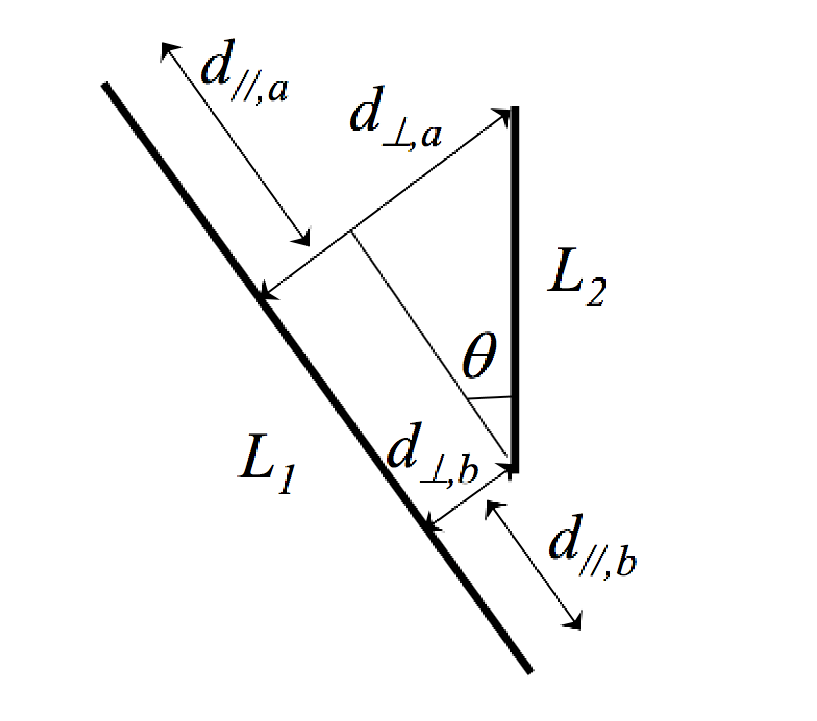
\includegraphics[width=0.43\textwidth]{Fig/chapter2/Hausdorff}
	\caption{霍斯多夫距离}
	\label{fig-chapter2-Hausdorff}
\end{figure}

\textbf{弗雷歇距离:}
弗雷歇距离通俗的讲就是狗绳距离。如图\ref{fig-chapter2-Frechet}所示人和狗的轨迹, 两者之间有一条狗绳约束。主人走路径A,狗走路径B,各自走完这两条路径过程中所需要的最短狗绳长度就是弗雷歇距离。
\begin{figure}
	\centering
	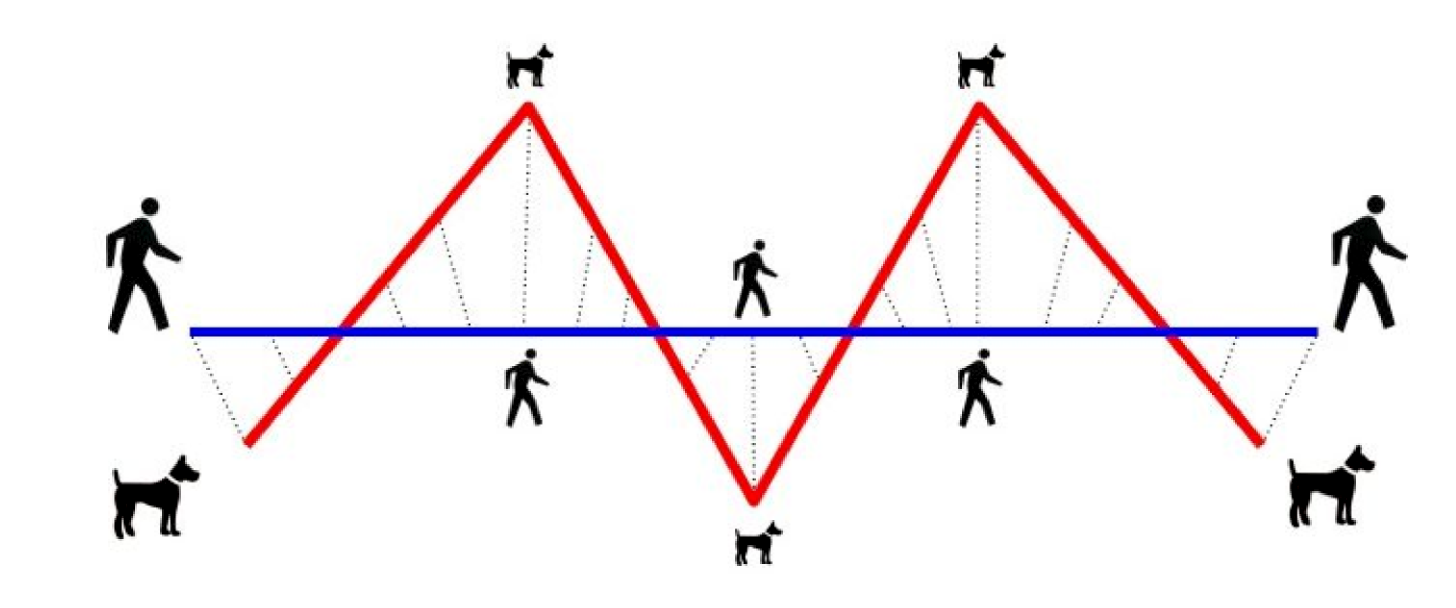
\includegraphics[width=0.73\textwidth]{Fig/chapter2/dogpeople}
	\caption{霍斯多夫距离}
	\label{fig-chapter2-Frechet}
\end{figure}

\subsection{语义轨迹距离}
语义轨迹的特点是将原始轨迹中的坐标映射到一个语义信息上,如给点标注为“学校”。从而使得原始的坐标序列变为语义信息的序列。现有语义轨迹度量方式的思想就是从语义和空间两个角度来考虑相似性,但它们的实现方式各不相同。

\begin{figure}
	\centering
	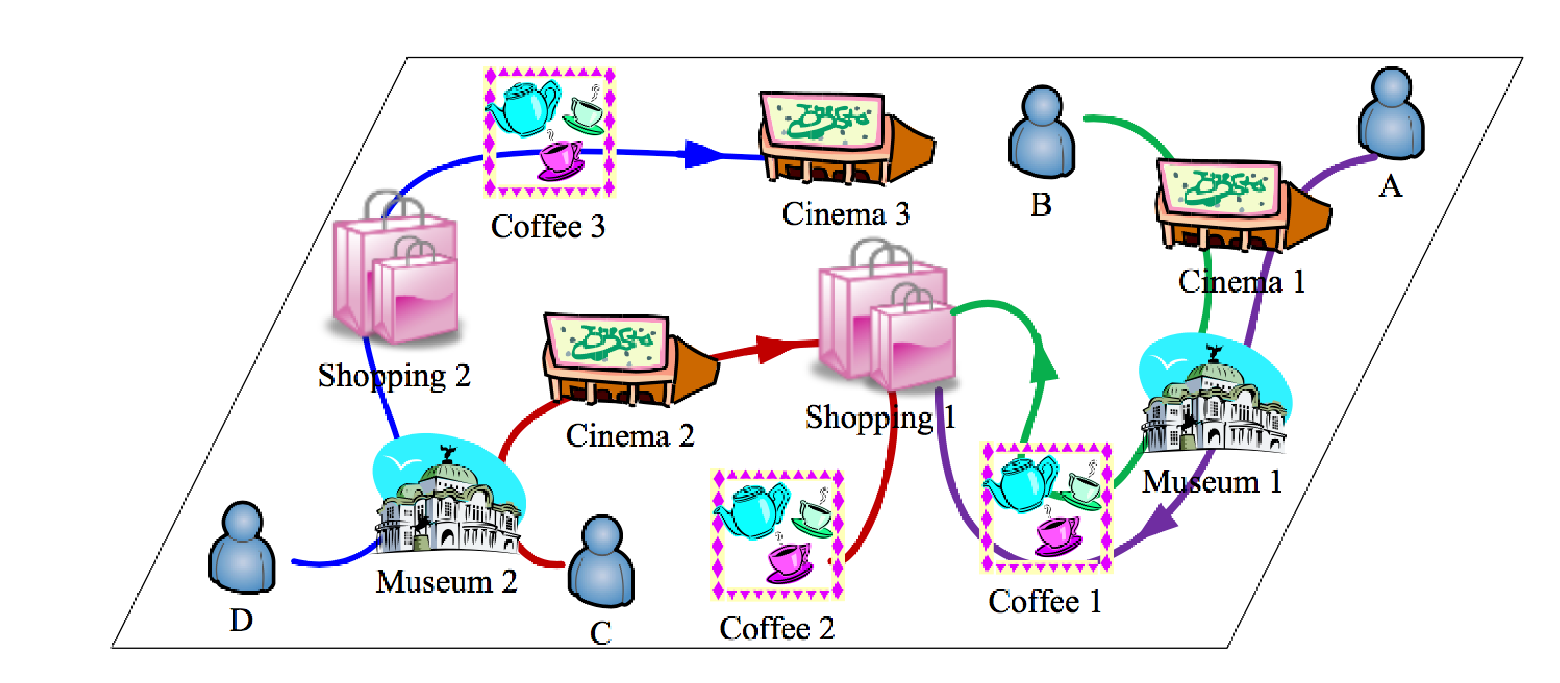
\includegraphics[width=0.73\textwidth]{Fig/chapter2/catagorySementic}
	\caption{基于分类属性的语义轨迹}
	\label{fig-chapter2-category}
\end{figure}
文献\cite{Xiao}提出了基于位置分类属性的语义轨迹分析方法。如图\ref{fig-chapter2-category}所示,该方法首先将POI分成博物馆、医院、学校等若干个类别,然后给原始轨迹的每个点赋予类别属性。最后使用类别属性的序列进行相似度计算。

文献\cite{Liu012}利用轨迹空间距离和语义距离的比值来作为最终两个轨迹的相似度。其计算方式如公式\ref{eq:ch2-Liu012}所示,其中$geoDist$代表了两条轨迹的空间距离,$semRatio$代表了两条轨迹间的语义距离。其空间距离考虑了轨迹中心点间的距离、轨迹长度的差别和轨迹间的角度。其语义距离使用最长公共子串距离除以短轨迹长度来表示。$\alpha$用于调节着空间和语义距离的比重。
\begin{eqnarray}\label{eq:ch2-Liu012}
totalDist(t_{1},t_{2}) =geoDist(t_{1},t_{2})\cdot \frac{1}{1+\alpha \cdot semRatio(t_{1},t_{2})}
\end{eqnarray}

文献\cite{ZhengYZXSZ15,Kaiser,ShangDYXZK12}给空间距离和语义距离以不同权重,并用它们的权重和作为轨迹或轨迹点的相似度。其定义形式如公式\ref{eq:ch2-add}所示。
\begin{eqnarray}\label{eq:ch2-add}
totalDist(t_{1},t_{2}) = \alpha  geoDist(t_{1},t_{2}) + (1-\alpha)  semRatio(t_{1},t_{2})
\end{eqnarray}
其中文献\cite{Kaiser}中要求被查询轨迹要完全包含待查询轨迹的所有语义信息。文献\cite{ShangDYXZK12}不是给每个点一个标签属性,而是给每条轨迹一个标签信息。而文献\cite{ZhengYZXSZ15}给出的是近似查询结果。

\section{$k$近邻轨迹查询}\label{sec-c2-topk}
关于$k$近邻轨迹查询的研究工作有很多,我们将这些工作分为两大类:集中式环境下查询和分布式环境下查询,并分别作介绍。

\subsection{集中式环境下查询}
轨迹数据上的$k$近邻查询,已经得到广泛研究。我们将这些工作分为:历史数据上的查询,轨迹流上的连续查询以及不确定轨迹上的查询。

\textbf{历史数据上的查询}

目前已经有一些针对历史数据的轨迹管理系统以支持轨迹查询\cite{BoteaMNS08,ChakkaEP03,Cudre-MaurouxWM10}。
Botea等\cite{BoteaMNS08}首先构建了针对轨迹数据的管理系统PIST。该系统将轨迹数据以点为基本单位构建空间索引。它首先统计轨迹数据在空间维度的分布,然后构建空间索引以对数据进行划分。接着对每个划分内部的数据根据时间维度构建索引。
Chakka等\cite{ChakkaEP03}提出了以子轨迹为基本单元的管理系统SETI。该系统同样首先根据统计数据构建空间索引。然后根据空间索引划分轨迹数据,并将每个划分内同一移动对象的子轨迹作为基本处理单元构建时空索引。该工作表明,基于子轨迹的索引策略比基于点的策略查询效率要高。进一步地,Philippe等\cite{Cudre-MaurouxWM10}提出了基于I/O开销模型的轨迹数据管理系统TrajStore以支持动态轨迹划分。TrajStore对每个划分内的子轨迹进行聚类并用簇中心来代表簇内所有轨迹,从而降低数据的存储开销。此外,它还使用了多种数据压缩技术以进一步降低存储开销。Wang等提出针对大内存服务器的轨迹数据系统SharkDB\cite{WangZZS15,WangZXZZS14,ZhengWZSLS18}。该系统提出了3种存储框架用以降低数据存储开销同时增大内存命中率。此外引入了分层索引以提高查询效率。
上述轨迹系统需进行功能扩展以实现近邻轨迹查询。

此外集中式邻轨迹查询已经得到广泛研究。
Agrawal等\cite{AgrawalFS93}首先使用离散傅里叶变换来转换轨迹数据并保留最开始的几个频率作为轨迹特征。原始轨迹上的$k$近邻查询,可通过先在特征值上的查询结果来进行剪枝,以提高查询效率。
Refiei等\cite{RafieiM02}使用傅里叶描述子来表示轨迹形状的边界,接着对每个形状计算出多维指纹信息并对指纹数据构建R树索引。最后使用指纹间的距离来近似原始轨迹间的距离。该方法计算出来的距离不受位置,方向和轨迹起始点的 影响。Pelekis等\cite{Pelekis}针对仅考虑空间维度和同时考虑时空维度两个方面定义了轨迹相似度,并分别提出了处理方法。此外,还提出了考虑速度、加速度和方向的方法。

Frentzos等\cite{FrentzosGPT07}提出了基于R树索引的查询算法用以处理近邻轨迹查询,并比较了当使用不同类型R树索引对查询效率的影响。Xu等\cite{GutingBX10}提出了基于剪枝-提炼的解决方案。在剪枝阶段其同样利用R树索引来进行剪枝。具体地,其为树的每个叶子节点设计一个时间独立且收敛的覆盖函数,并在查询过程中通过计算查询对象与节点包围盒的距离更新该函数值。最终返回满足查询条件的轨迹段。在提炼阶段,将上一步获得的轨迹段按照到达时间进行排序并合成完整的轨迹。文献\cite{KolliosGT99}提出了最近邻轨迹预测问题,其目标是预测接下来一段时间内,与给定查询轨迹最相似的轨迹。其使用kd树和B+树来构建对偶索引以提高预测速度。
Ranu等针对轨迹数据的异频采样和无固定采样频率的问题,设计了新的轨迹距离计算方法EDwP,并根据该距离设计了新的索引策略用于剪枝查询结果。Chen等\cite{ChenSZZX10}提出了$k$最好连接轨迹轨迹查询问题。其目标是针对给定的一组有序或无序位置信息,找出$k$条其某条采样子轨迹与给定查询最匹配的轨迹。该算法首先给出了满足查询条件的轨迹距离定义方式,然后基于点最优匹配的查询算法。该算法针对索引树,提出了基于查询开销的最优优先和深度优先两种查询策略。最后比较验证了两种策略的性能。

此外,Skoumas等\cite{Skoumas}使用豪斯多夫距离来计算轨迹段的相似度,并用轨迹段的累加值作为最终轨迹间的相似度。因此,其首先提出了一个基于优先队列的剪枝算法$ExactKNN$。该算法通过前几个时间戳上的数据来构建相似度上、下界,并维护一个上界的优先堆(大堆),当堆顶元素下界大于次小元素的上界时,则该元素加入最终的结果集并从堆中移除。否则,不段对堆顶元素增加更多时间戳内地数据以更新上、下界。该算法直到找出$k$个结果才会停止。该方法,虽然能找出精确的结果但也存在着迭代次数多的问题。为此,提出了两个近似算法以提高查询效率。第一个是基于简化轨迹的算法。其首先使用\cite{Zhao1997LINEAR}所提技术简化轨迹,简化后的轨迹近保留有限个时间戳上的数据。然后对简化轨迹调用$ExactKNN$算法。该方法虽然会导致部分结果不正确,但能大大降低计算开销。第二个是基于先验概率的加速算法。其首先计算出轨迹段的分布概率,接着在计算轨迹段距离上、下界的过程中引入该分布。使得包含先验概率高轨迹段的轨迹得到优先扩展。


目前,还有一些针对语义轨迹的$k$近邻查询研究\cite{Xiao,Kaiser,WangBCSSQ17}。Xiao等\cite{Xiao}提出了基于语义轨迹的$k$近邻查询。其首先将原始的位置序列轨迹通过停留区查找算法变成停留区序列(即语义轨迹)。接着对语义轨迹提出 了匹配的定义并基于次给出两条语义轨迹的距离度量。最后,将语义轨迹间距离度量的问题转化为图的构建问题。
Zheng等\cite{Kaiser}提出了$k$近邻活动轨迹的查询研究。其目标是给定一组位置序列,每个位置带有多种活动标签(这样的序列称为活动轨迹)。其目标是从用户活动轨迹数据集中找出与给定序列距匹配度最高的$k$条。为此,其分别定义了基于点和轨迹的匹配度量方式,接着给出了匹配距离的下界并证明了通过下界能快速剪枝候选。最后给出了两种算法以分别处理查询点集合有序和无序的场景。
该工作所提查询要求返回的轨迹必须完全包含所有待查询活动标签的类别,只要有一个标签不包含,则认为返回的轨迹与查询不相似(相似度为0)。
Wang等\cite{WangBCSSQ17}等在此基础上进行了改进,认为一条轨迹包含待查询轨迹内容标签越多,则相似度越高。此外,该工作还给每个位置上的标签赋予一定的权重以满足不同用户的需求。为解决所提查询,他们首先提出了相似度上、下界的增量式算法。但该方法存在着迭代次数多的问题,为此提出了动态扩展的策略以给每个查询点以不同的扩展范围。进一步地,为解决每次扩展中需要对索引树进行深度遍历的问题,提出了两层阈值算法,以保证一次搜索就能找出满足条件的候选。

\textbf{轨迹流上的连续查询}

此外,Sacharidis等\cite{SacharidisSS14}还研究了轨迹数据流上的$k$近邻轨迹查询。该工作使用滑动窗口来处理轨迹数据流,并使用窗口内每个时段点的距离的聚集值(最大、最小、累加、均值等)作为轨迹相似度。其首先提出了基于事情模型驱动的通用处理方法BSL。该方法关注如下三类事件:(1)待查询移动对象的位置变化(Query location updates,$QUpd$),(2)被查询移动对象位置的变化(Object location updates, $OUpd$)含新位置到达和旧位置过期,(3)移动对象与被查询移动对象位置过期(Object distance expiration, $OExp$)。BSL为查询对象保留最后时刻的位置,为其他移动对象保持最后的位置和窗口内的距离序列(每个时间戳对应一个其余查询对象的距离)。此外还维护了一个事件列表以便及时删除过期的位置信息。当事件某一类型事件到达时,按照其设计的方案更新轨迹间的距离。接着,提出了改进算法XTR用以去出无用点(不会影响到最终轨迹间距离值的点)以减少遍历时间。最后,提出了基于移动对象最大以速度改进算法HRZ。该方法利用最大移动速度约束,以剪枝候选。XTR和HRZ这两个改进方法只适用于使用最大和最小距离作为轨迹距离的情况。

Bakalov等\cite{BakalovT06}研究了轨迹数据流上的连续join查询。其目标是针对两个不断变化的轨迹数据集,数据集间的轨迹进行两两相似度匹配并返回最相似的,且相似度有轨迹空间邻近度决定。其首先使用轨迹近似技术来降低数据的维度并对近似轨迹构建空间索引。接着对近似轨迹设计了距离下界用以进行剪枝。针对连续查询,设计了两阶段处理方法。第一阶段根据当前窗口内的数据初始化查询结果。在该阶段使用索引来降低匹配的个数并利用下界得到近似结果。第二阶段针对数据的变换,持续检查结果集并作出更新。

\textbf{不确定轨迹上的查询}

首先,隐藏时间序列数据和不确定数据流上的概率相似度查询\cite{LianCY08,YehWYC09}上的查询已经被广泛研究。这类工作首先提出概率距离的计算方式,其需要设置两个阈值参数。一个是距离阈值$\gamma$另一个是概率阈值$\tau$。其查询目标是返回与查询轨迹距离小于$\gamma$的概率超过$\tau$的轨迹。因此,查询结果对这两个阈值比较敏感。阈值作轻微改变可能查询结果的大小和内容发生较大变化。

此外,一些专门针对不确定轨迹数据上的查询也被提出\cite{TrajcevskiTDSC09,Ma2013KSQ}
文献\cite{TrajcevskiTDSC09,Trajcevski2011}研究了给定不确定轨迹数据集上的连续近邻查询。其假设查询与被查询的轨迹都是不确定的,但轨迹在给定范围内满足一定的概率帆布。其目标是不断返回与待查询轨迹概率距离最高的$k$条轨迹,并找出结果集内容或顺序发生变化的时间点。其主要思想是构建一棵几何对偶的树索引以剪枝候选。
Ma等\cite{Ma2013KSQ}研究了不确定轨迹数据上的$k$近邻轨迹查询。其与文献\cite{TrajcevskiTDSC09}的研究内容差别是其给定的查询轨迹是确定的。
该工作假设所处理的轨迹数据位置具有一定的误差,且误差满足一定的概率分布。为度量两条不确定轨迹的相似度,其首先提出了$p$距离。给定轨迹$x$与查询$\cal Q$的$p$ 距离由其他比$x$离$\cal Q$更近的轨迹的概率距离和表示。即$x$离$\cal Q$越近,越少的轨迹比$x$更近。接着提出了基于空间网格划分的$UTgrid$索引,并对每个网格内的轨迹构根据时间维度构建1维R树索引。最后设计了针对不确定轨迹的查询算法,该算法利用$UTgrid$进行剪枝以达到提高查询效率。
与以上工作不同地是,Li等\cite{LiLSF11}研究了基于路网的不确定轨迹查询。该工作中假设移动对象在路网中的移动速度未知。因此如何预测哪些轨迹会成为将来的候选集成为难点。

\subsection{分布式环境下查询}
为处理轨迹大数据,分布式环境下的$k$近邻轨迹查询得到越来越多的研究。我们将从分布式轨迹数据查询系统和分布式近邻轨迹查询两方面进行介绍。

\textbf{分布式轨迹数据查询系统}
近10年来,随着Hadoop\footnote{http://hadoop.apache.org/}、OpenStack\footnote{https://www.openstack.org/}和Spark等大数据处理开源系统的普及,在这些系统上构建轨迹轨迹数据管理系统成为新的方向。目前,已经出现了大量基于这些开源分布式平台的轨迹数据管理系统以支持轨迹查询。

Lu等\cite{LuG12}设计了并行的空间数据DBMS系统Parallel-Secondo。该系统在每台节点上使用传统的空间DBMS来实现数据存储和查询实现,仅使用Hadoop作为结点间任务调度器。
Ma等\cite{MaYQZ09,YangMQZ09}首先提出了基于Hadoop的轨迹数据管理系统。为提高查询效率,其构建了两类索引。第一类是基于空间的索引,用于将数据按空间维度划分。此类索引能加速带有空间约束的查询,但如果查询某个移动对象的轨迹,则需要遍历许多数据分区。为此设计了第二类基于移动对象的倒排索引,该索引中存储了每个移动对象的轨迹数据是存储在哪些数据分区上。Clost\cite{TanLN12}通过建立一个多层索引用以数据划分。同时,其支持数据的批量增加。
SpatialHaddop\cite{SpatialHadoop}系统是基于Hadoop的典型空间数据管理系统。该系统从以下四个方面对Hadoop进行了改进以满足空间数据查询的需求。
(1)提供了基于多种索引树的存储策略。首先根据全局索引用以完成数据划分,其次在每个数据块内支持块内局部空间索引。这种全局-局部的索引方式能大大减少I/O开销;(2)设计了新的文件读写方式,以支持对块内索引数据的读写;(3)设计了多种查询接口,以方便开发这进行查询调用;(4)设计了基于Pig Latin的查询语言,以方便普通用户实现查询功能。但SpatialHadoop只能用来管理静态数据,当新的数据到达时,需要将整个数据集重新划分,因而开销较大。
AQWA\cite{AlyMHAOEQ15}是其改进版本,允许数据动态添加。AQWA建立了新的数据划分模型,同时考虑了用户查询和数据分布对划分的影响。以上系统最终将查询需求,变成定制的Map/Reduce\cite{DeanG04,mapreduce}任务。


此外,还有一些基于Hadoop组件或类Hadoop系统的时空数据管理系统。Ablimit等\cite{AjiWVLL0S13}等提出了基于Hive\footnote{https://hive.apache.org/}的轨迹管理仓库Hadoop-Gis,其通过网格索引以提高范围和join查询的效率。MD-HBase\cite{MDHBase}和R-HBase\cite{RHBase}是两个基于HBase\footnote{https://hbase.apache.org/}设计的实时时空数据管理系统。MD-HBase使用Z-Curve空间填充曲线来划分数据空间。接着对所用划分子空间使用四叉树或k-d树索引来构建空间索引。R-HBase使用了局部性更好的希尔伯特空间填充曲线来划分数据空间,并使用R树来构建空间索引。这两个系统借助了HBase的特性可支持数据的实时插入和修改。Geomesa\cite{Geomesa}与以上两个系统类似,可以快速部署到类似HBase的键值对存储系统中,且其从语言层定义了空间查询操作接口以方便用户调用。相较于以上系统,Elite\cite{XieMCDJ16}专门设计用于处理不确定轨迹数据并提供了丰富的不确定查询接口。

尽管基于Hadoop生态圈内系统构建的分布式轨迹管理系统能满足轨迹查询的需求,但也面临着由于I/O开销较大,导致无法提供实时、高吞吐率的查询服务。为此,出现了许多基于Spark等分布式内存的时空数据管理系统,以提供实时和高吞吐率的查询服务。
SpatialSpark\cite{SpatialSpark}和GeoSpark\cite{GeoSpark}是最早的两个基于Spark设计的专门用来处理空间数据查询的系统。其中SpatialSpark专门用来出列空间join查询。 GeoSpark设计了一个新的数据结构SRDD用来表示分布式空间数据。SRDD使用全局空间索引来划分数据,且支持每个分区内部构建局部索引。进一步地, LocationSpark\cite{Locationspark} 提出了使用布隆过滤器来 解决数据分布倾斜问题。
最新地,Dong等人提出了新的基于SparkSQL的空间数据管理系统Simba \cite{Simba}。相比现有基于Spark的系统,Simba从查询解析到查询执行都作了优化。其中最明显的是在其查询执行计划设计方面使用了空间索引等其技术来提高查询效率。此外,它还从语言层提供了用户查询接口。相比以上系统,TrajSpark\cite{TrajSpark}是专门设计用来处理轨迹数据的系统。其实现了3类典型的轨迹查询接口,并利用全局-局部索引策略以提高查询效率。
此外,目前还存在着专门用于对时空数据进行复杂分析的系统\cite{OceanST,STORM}。STORM\cite{STORM}设计用来处理交互式近似查询。相比于已有的设计用来精确查找的系统,该系统能在查询提出后,通过逐渐增加采样数据以不断以一定置信度给出查询结果。用户根据系统不断精细的结果随时可以停止查询。OceanST\cite{OceanST}同样适用采样技术来获得查询近似结果,且能处理数据不断增加的场景(STORM仅能处理静态历史数据)。此外,它还提供了丰富的查询接口用以满足各种查询需求。



\textbf{分布式近邻轨迹查询}

目前,已经出现了基于Map/Reduce并行计算框架下时间序列相似性问题的研究工作\cite{kimICDE2012,kimICDE2012}。文献\cite{kimICDE2012}研究了基于Map/Reduce框架的集合数据的join查询问题,其目标是减少数据节点间的通信问题。
文献\cite{kimICDE2012}针对Map/Reduce框架下数据集的top-$k$join查询问题进行了研究。其首先提出了基于分治法和分支限界法的两种实现策略。接着提出了全部配对划分和有限配对划分的数据划分策略以减少map和reduce任务间的通信开销。
此外,还有一些使用多通用计算图形处理器(GPGPUs)并行计算框架的工作\cite{GowanlockC14,Zhang2012U2STRA,LealGZY15}。其中
文献\cite{GowanlockC14}研究了范围查询即找出与查询轨迹距离小于给定阈值的轨迹。其提出了新的适用于GPU的索引结构有一替代传统的R树索引。给定一个查询集合,它提出了多个方法以将查询分成若干互相独立的批次以得到更好的内容命中率和降低计算的开销。
文献\cite{Zhang2012U2STRA}构建了针对轨迹数据的管理系统并研究了基于霍斯托夫距离的轨迹相似度join查询。其主要贡献在于设计了四层轨迹数据表现方式并设计了一个3层所以架构用以提高查询效率。Leal等\cite{LealGZY15}首先提出了基于霍斯托夫距离的$k$近邻轨迹查询算法TKSIMGPU,其主要研究目标是使得各个计算线程负载均衡。Top-KaBT\cite{LealGZY16}是TKSIMGPU的改进版本,其提出了轨迹间霍斯托夫距离上、下界 用以减少需要计算精确距离的候选数。

针对协调者-远程结点分布式架构,一些轨迹序列top-$k$查询算法已经被提出\cite{CIKMSimilarity,SmartTrace,crowdsourced}。文献\cite{CIKMSimilarity}研究针对手机信令轨迹数据进行了$k$近邻研究。其将每个手机基站看作远程结点,用户移动的过程中会经过不同的基站,因而其轨迹数据会分成若干段并保留在不同的节点上。为处理针对这一数据的查询,其提出的算法在每个远程结点保存子轨迹距离的上、下界以提高查询的效率。
Smart Trace\cite{SmartTrace}和 Smart Trace+\cite{crowdsourced}两个系统是针对众包场景下的查询。其将每个用户的手机看作远程结点,因而每个远程结点只有一条轨迹数据。针对这一场景,Smart Trace提出了基于LCSS距离的上界用以查询时间和能量消耗。进一步地,Smart Trace+还提出了新的下界并提出了结合上、下界的处理算法。以上工作均是将提高查询效率作为首要目标,并未深入所提算法在通信问题上的开销。


为解决协调者-远程结点架构下,$k$近邻轨迹查询中的通信开销过大的问题。基于多粒度概要数据的方法已经被提出\cite{PapadopoulosM01,LeeWave,DTKST,bandwidth,bandwidth}。Papadopoulos等\cite{PapadopoulosM01}首先对分布式时间序列进行了$k$近邻查询研究,并提出了4种基于协调者-远程结点的方案以求在提高时间效率的同时降低通信开销。但该方法仅能降低从远程结点返回给协调者结点的数据开销,协调者结点仍需要将待查询时间序列发送给所有远程结点,而该开销是所有算法通信开销的主要部分。因此,其并未彻底解决通信开销过大的问题。
Yeh等 \cite{LeeWave}提出了用于降低通信开销的算法LEEWAVE。其使用小波变换的数据压缩放,将原始时间序列数据变换成多粒度的概要数据。LEEWAVE算法中协调者结点将概要数据由粗到细发送给远程结点,远程结点根据概要数据计算候选轨迹与查询轨迹欧式距离范围的必要参数,并将参数发送给协调者结点用以计算距离上、下界并进行剪枝。其根据多粒度数据不断缩小距离范围的方法能大大降低通信开销。文献\cite{KashyapK11,DTKST}提出了更紧的下界,因而能打到更好的剪枝效果。文献\cite{LeeWave,KashyapK11,DTKST}都是基于哈尔小波变换的压缩方式,而该方式仅适用于距离度量方式是欧式距离的场景。
此外,文献\cite{bandwidth}提出了针对DTW距离的算法,该算法引入多粒度包围信封以作为概要数据,并根据该概要数据计算下界。此外,使用级联下界的方式以进一步降低计算开销。而文献\cite{bandwidth}在其基础上提出了新的上界,并引入了同时根据上、下界进行剪枝的算法MDTK。MDTK算法引入了边剪枝边过滤的思想用以加快下界的计算速度。以上工作都是针对某一具体距离度量方法提出相应的基于概要数据的距离上、下界,并未考虑如何扩展到其他轨迹距离的度量方式上。为此,亟需提出通用的方法,以解决分布式$k$近邻轨迹查询。


\clearpage
\phantom{s}
\clearpage
\chapter{基于集群的分布式轨迹管理}\label{chapter:system}
本章主要介绍如何在集群内构建轨迹数据管理系统并提供实时的查询结果。首先,章节\ref{sec-c3-background}介绍了背景知识。其次,
章节\ref{sec-c3-system}介绍了本文设计的系统架构及系统的实现。
然后,章节\ref{sec-c3-exp}实验验证了系统的性能。最后,小结本章的研究内容。

\section{引言}\label{sec-c3-background}
\subsection{背景知识}
基于分布式集群的数据管理和分析方法是当前解决大数据问题的首选方案。分布式集群内的存储和计算方案通常采用主从式架构,即主节点负责管理数据的元数据和任务的分发,从节点负责存储数据的一部分并负责对这一部分数据进行分析。
Hadoop 和Spark是基于主从式架构设计的当前最流行的大数据处理系统。这两个系统的最大区别是Hadoop是基于磁盘的数据处理方式。
每当有新的查询或分析任务产生时,存储在磁盘上的数据需要先被读取到内存上再做分析。因此,基于Hadoop构建的轨迹数据管理系统如Truster \cite{YangMQZ09}和Clost \cite{TanLN12}等都面临着I/O开销过大问题,因而无法提供实时的查询分析结果。而Spark是基于内存的处理方式,在进行数据分析前,所有数据可以被加载进入集群的内存中(Spark通过off-heap技术处理数据内存放不下的情况)。
新的查询过来后,可以直接从内存里面查询数据,有效地避免了I/O开销。因此,Spark成为当前提供快速数据分析的主要工具。

鉴于Spark的高效性能,本文考虑使用这一系统来进行轨迹数据管理和查询实现。在此之前,我们将首先对Spark作一个概括介绍。
Spark是一个通用的并得到广泛使用的用于处理大数据的集群计算引擎。其提供了丰富的Scala、Java和Python调用API接口,以方便用户操作数据。该系统一经提出,围绕其展开的用于进行内存数据分析的生态圈系统便得到广泛关注。这些系统提供了丰富的数据处理功能,包含数据仓库(Spark SQL)、流数据处理(Spark Streaming)、图数据处理(GraphX)和机器学习(MLlib)。

Spark提供了一个高效的基于分布式集群内存的数据抽象:
弹性分布式数据集(Resilient Distributed Dataset, RDD)。每个RDD可以看做是一个Java或Python中的对象集合,这些对象按照一定的方式分布在集群内的机器上。用户可以通过函数式编程API(如map、filter、reduce)来实现对数据的操作。RDD具有较好的容错性,因其可以通过依赖图以重新计算部分算子以恢复丢失的分区内的数据。
所有的RDD可以既可以被缓存到内存中又可以被显示的保持到磁盘中以加速数据的重复利用并支持迭代计算。RDD上的算子可以分为两类:一类 是转换(Transform),其操作在一个RDD上得到另一个RDD,如map、filter、union等。另一类就是行动(Action),其返回结果或是把结果持久化起来,如count、collect 、save。其中转换类算子采用的是懒策略,即其提交后不会立马执行,而是等到行动算子被提交时才会触发。

\subsection{基于Spark的时空管理系统}
目前,已经出现了些利用Spark构建时空数据管理系统。本小节将对这些系统作简要介绍。

\textbf{GeoSpark.}GeoSpark 扩展了Spark以处理空间数据。它提供了新的适用于空间数据的抽象模型SRDDs以及对空间对象的操作算子。GeoSpark提供空间范围查询、$k$近邻查询和空间join查询。除此之外,它允许在每个数据分区提供一个局部索引(四叉树和R树)。值得注意的是,Spark允许开发者构建任意对象类型的RDD(如关于点、多边形和圆等对象)并提供对应的空间操作算子。尽管GeoSpark能够使用局部索引提高查询速度,但其不支持全局索引。此外,它支持2维空间数据,不能处理带有额外属性的空间对象(如带有用于描述信息的对象)。
%换句话说,GeoSpark就是一个运行在Spark之上的

\textbf{SpatialSpark.}SpatialSpark 在 Spark之上实现了一些用于分析空间数据的接口。特别地,SpatialSpark提供了空间范围查询和join查询(使用如``相交''和 ``包含''作为约束)的接口。其使用一个确定的kd树或网格索引来划分数据和并提高查询效率。尽管如此,SpatialSpark只提供2维数据上的操作,且不支持对RDD构建索引。

\textbf{Simba.}Simba扩展了SparkSQL以提供类SQL空间查询。特别地,它提出了IndexRDD以管理多维空间数据。IndexRDD在每个分区包含一个局部空间索引,并为所有分区构建了一个全局索引。Simba提供了空间范围查询、$k$近邻查询和空间join查询等查询接口。为进一步提高查询效率,Simba从逻辑层(查询解析)和物理层(查询计划)两方面进行了优化。相比于前面两个系统,Simba能处理多维数据。

\textbf{注意.}上述系统都是针对空间对象(点、线、面)数据进行管理。而轨迹数据除了空间维度还有时间维度以及移动对象标识这两个重要属性。这使得我们在存储数据时,不但要把空间靠的近的轨迹放到一起,还要把时间邻近的以及同一个移动对象的数据放到一起。


\section{TrajSpark系统设计及实现}\label{sec-c3-system}
本节将介绍在Spark之上构建的轨迹数据管理系统TrajSpark。

\subsection{系统架构}
\begin{figure}
	\centering
	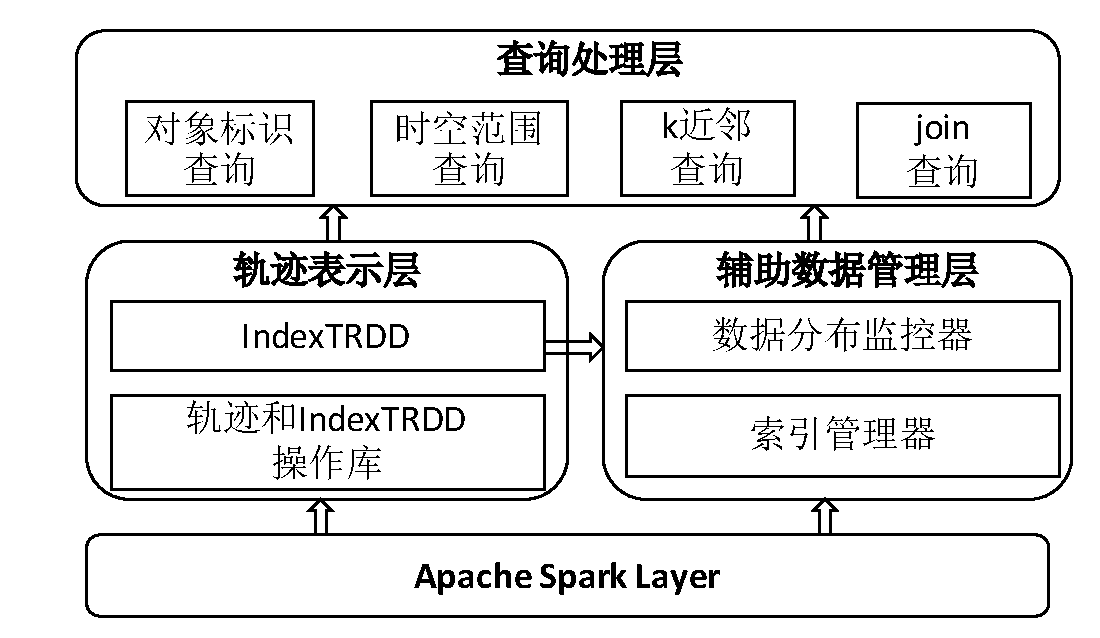
\includegraphics[width=0.73\textwidth]{Fig/chapter3/overview}
	\caption{剪枝示例}
	\label{fig-chapter3-architecture}
\end{figure}

TrajSpark系统架构如图\ref{fig-chapter3-architecture}所示,其由如下四层构成: (1)Apache Spark层,该层由Apache Spark提供的RDD及其常用操作构成;(2)轨迹数据表示层,该层介绍了对轨迹数据的抽象表示结构IndexTRDD;(3)辅助数据层,该层监控管理数据添加导致的数据分布变化,并负责指导对新数据的划分;(4)查询处理层,该层对三种典型轨迹查询进行了算法设计。具体地:

\begin{itemize}
	\item \textbf{Apache Spark 层:}  
	该层是整个系统的基础,其继承自Apache Spark,故不作详细介绍。
	
	\item \textbf{数据表示层:} 在该层,我们首先为轨迹设计了结合列存储形式的轨迹表示方法以达到压缩数据的目的。在TrajSpark系统中,轨迹以轨迹片段的形式存储,一条长轨迹将被切分成多条轨迹片段,而时空相邻的轨迹片段将被放到同样的数据分区中。
	为此,我们设计了基于轨迹片段的数据表示结构IndexTRDD,并提供了丰富的轨迹查询算子。为提高轨迹查询效率,TrajSpark为IndexTRDD维护了全局和局部两层轨迹索引。其中全局索引维护了所有分区的时空信息,而局部索引维护了每个分区内部轨迹的信息。该层是整个系统的核心。
	
	\item \textbf{辅助数据层:} 这一层维护了两种系统的全局信息。第一种就是轨迹数据的分布信息,其由数据分布监控器(Data Distributor Monitor)管理。随着数据不断装载入系统中,数据的分布会随之发生变化。TrajSpark通过监控这一变化并设计合理的数据划分方式以达到数据均衡的目的。第二种就是全局索引,其由索引管理者(Index Manager)维护。索引管理者运行在主节点上,用以管理数据的全局索引。当数据加载进后,索引管理这将更新全局索引。
	
	\item \textbf{查询处理层:} 这一层主要实现了两类基本轨迹查询以及轨迹$k$近邻查询。此外,用户可以通过基本函数接口实现更加复杂的查询。
\end{itemize}

\subsection{数据表示层}

\textbf{轨迹片段表示}
	
	原始来自轨迹GPS日志中的轨迹数据往往以轨迹点集的形式保存。因而,原始信息可以看作包含如下属性的表格$(MOID$, $Location$, $Time$, $A_{1}$, $\cdots$, $A_{n})$。其中$MOID$是移动对象的标识,  $Time$记录了轨迹点采集的时间、 $Location$代表轨迹点的位置。其他属性根据数据源的不同而变化。基于Spark的一个简单轨迹数据管理实现方案就是将轨迹数据看作由轨迹点构成的RDD。但该方案会导致数据的冗余,比如一个移动对象出现100次,则其标识将会重复100次。还有当连续采集的过程中,移动对象位置没有发生变化时,该位置仍然会被保存多次。
	除了数据冗余外,文献\cite{ChakkaEP03}表明基于轨迹片段的表示方式相比基于点的方式能显著提高查询效率。
	
	TrajSpark采用基于轨迹片段的方式管理轨迹数据。其将时空相邻的轨迹点聚集到统一数据分区中。此时,一条长轨迹可能被分割成若干段并存储在不同的分区上。在每一个分区内部,可以使用基于列存储的数据表达方式并结合数据压缩手段。实现这一目的存在两点挑战:
	(1)如何为非结构化的轨迹数据设计列存储的数据结构;(2)如何对列存储的轨迹数据进行压缩且不损害数据查询的效率。
	\begin{figure}
		\centering
		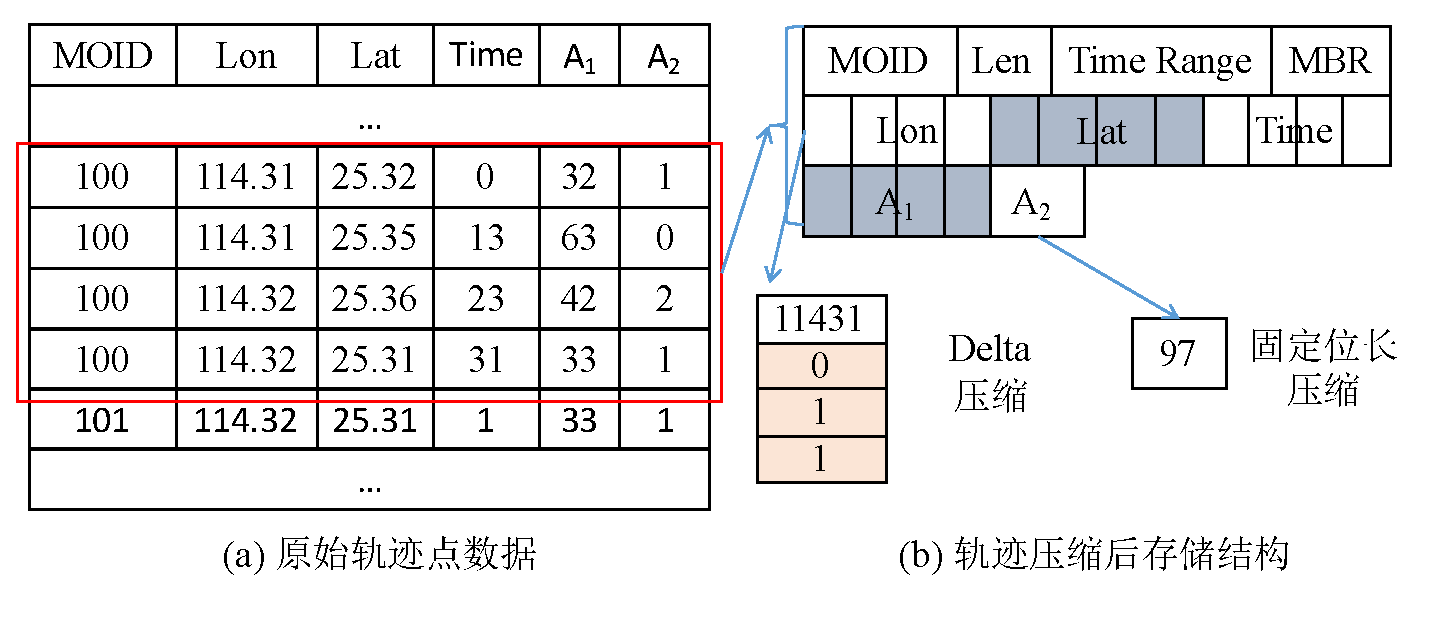
\includegraphics[width=0.95\textwidth]{Fig/chapter3/compress.eps}
		\caption{轨迹片段表示}
		\label{fig:TrajFormat}
	\end{figure}
	
	TrajSpark的实现方法是:在每一个分区内,先将所有轨迹点按照移动对象标识进行分组。接着属于同一移动对象的轨迹点按时间顺序进行排列,并得到一个轨迹片段。接着,将对每一个轨迹片段按
	图\ref{fig:TrajFormat}(b)所设计的表示方式进行压缩处理。在这种方式中,同一属性的值将被连续存放并压缩存储。其中针对数值型熟悉,如坐标位置等,使用差值压缩;对于枚举类型属性,使用固定为压缩。如图中$A_{2}$属性,其只有3个可能性的值即0、1和2。此时我们只需使用两个二进制位就能完成数据的存储。对于字符串属性,使用$gzip$进行压缩。压缩完所有数值后,我们为一条轨迹保留额外的概要数据,概要数据包含移动对象的标识、轨迹长度和(时空)最小包围盒信息。使用概要数据能对查询进行有效剪枝。最终,分区内轨迹点被转换为压缩好的轨迹片段,并使得整个轨迹数据集成为以轨迹片段构成的RDD(称之为TRDD)。
	
\textbf{轨迹片段索引}
	
	\begin{figure}[t]
		\centering
		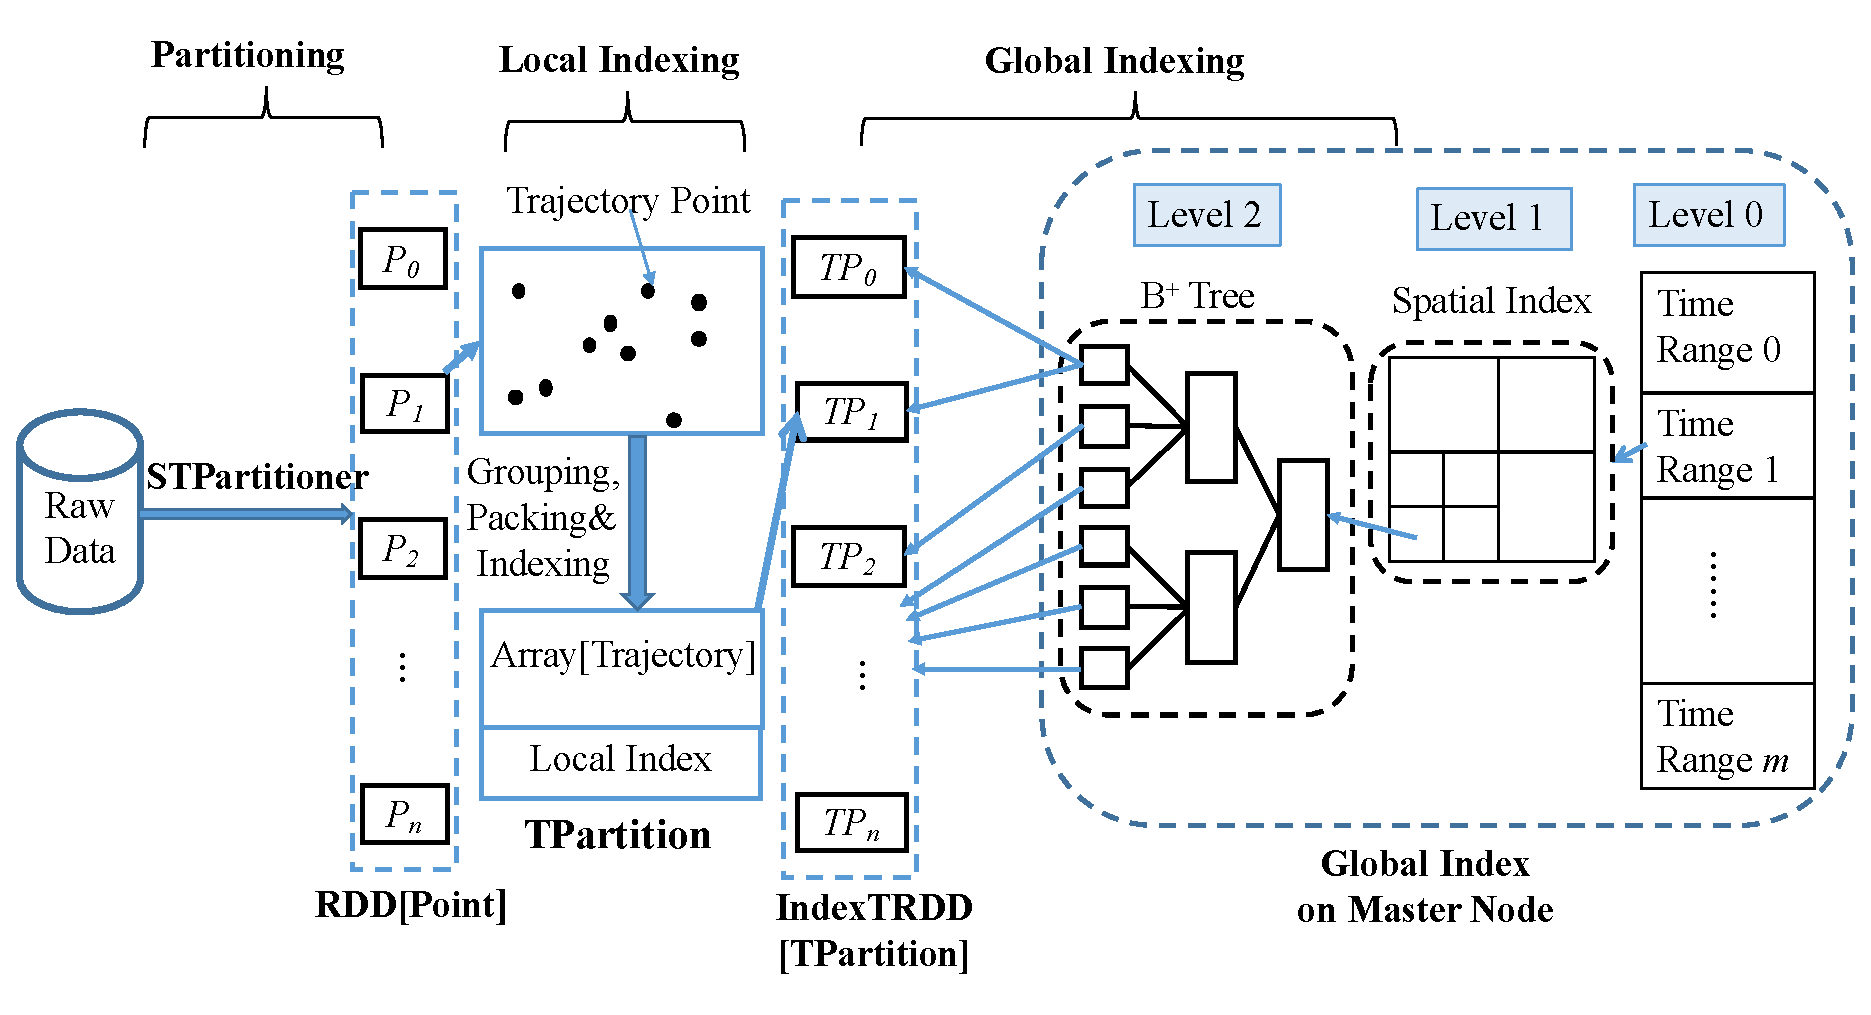
\includegraphics[width=0.95\textwidth]{Fig/chapter3/indexConstruct.eps}
		\caption{轨迹索引构建}
		\label{fig:index}
	\end{figure}
	
	前面,我们介绍了如何将原始的GPS记录转换成基于轨迹片段的TRDD。但TRDD对于给定的任意查询需要遍历整个数据集才能找到结果,因而CPU开销较大。为此,我们需要引入索引结构以提高查询效率。TrajSpark提出了IndexTRDD这一结构以支持索引。IndexTRDD首先通过在TRDD每个分区内引入针对轨迹标识的局部哈希索引,从而使得针对给定轨迹的查询复杂度降为常数级。进一步地,我们在IndexTRDD的分区之上构建了全局索引,以便查询执行时对不必要的数据分区进行剪枝。图\ref{fig:index}介绍了构建索引的整个数据流程,其包含:\emph{数据划分(Partitioning)}, \emph{局部索引构建(Local Indexing)}和\emph{全局索引构建(Global Indexing)}三个阶段。接下来将对这三阶段进行详细介绍。
	
	\emph{数据划分:}该阶段,TrajSpark将原始轨迹日志数据从磁盘装载进入磁盘形成一包含轨迹点对象的RDD。接着,我们需要对其进行数据划分以达到如下效果:(1)\textsf{数据局部性},即时空相邻的轨迹点需要划分到同一个数据分区中;(2)\textsf{负载均衡},各数据分区的数据量尽量相等;(3)\textsf{分区大小约束},每个分区数据大小要适中,以避免内存过载。尽管Spark本身提供了范围和哈希两种数据划分方法,但它们都是针对一维的数据进行划分。而轨迹是多维数据,这两种方式无法简单应用到轨迹划分中。为此,我们设计了新的针对轨迹的划分方法STPartitioner,该方法首先使用一颗四叉树或kd树来划分轨迹点。该索引树从原始轨迹的空间分布学习出来,以保证树的叶子节点所包含的轨迹点数量比较接近。当索引树构建好后,STPartitioner使用叶节点的边界进行数据划分。划分后,同一时空范围内的点被聚集到一起。
	为了保证每个分区大小适中,TrajSpark将聚集在一起的轨迹点根据移动对象标识或时间划分成若干大小相近的数据分区。
	
	\emph{局部索引构建:}经过数据划分后,轨迹数据集可看作是一个按时空划分好的点对象构成的RDD。在本阶段,我们首先将此RDD经过分组、排序和包裹以构建成以轨迹片段组织的TRDD。接着,为每个数据分区的头部添加一个局部哈希索引,用于将移动对象标识跟对应的轨迹片段映射起来。我们将这种包含索引及轨迹片段的分区称为TPartition。此时,整个数据集可看作由TPartition构成的RDD。我们称此时的RDD为IndexTRDD。最后,主节点收集每个分区的标识(每个数据分区都有一个特别的标识符)、分区所含数据的空间范围和时间范围等信息以便构建全局索引。
	
	\emph{全局索引构建:}本阶段,根据收集到的分区信息在主节点构建全局索引。全局索引的格式如图\ref{fig:index}所示,是一个三层混合索引。数据首先根据其时间维度信息被第0层粗粒度时间范围所划分。同时,每个粗粒度时间范围对应着一个第1维空间索引(STPartitioner就是根据这个空间索引对该时间范围内数据进行空间划分)。每个叶子节点所对应的空间范围可能包含若干数据分区,我们使用第2层B+树索引对这些分区根据时间维度进行管理。当第一批数据加载入系统后,第0层索引只包含一个时间值(时间段的起始时间),第1层空间索引即为数据划分所用的索引。我们收集每个分区的时间和空间信息以构建第2层索引。TrajSpark将全局索引保存在主节点的内存中并维护该索引的更新。即使当轨迹数据量很大时,我们的全局索引仍然只需消耗较少的存储空间,因而能以较低的内存开销放在主节点上。

\subsection{辅助数据层}

\textbf{数据分布管理器}

在真实的应用场景中,轨迹数据集会随着数据周期性的加载而不断变大\cite{AlyMHAOEQ15},从而导致数据的空间分布也发生变化。如何对新来的数据进行有效划分成为新的难点。一方面如果始终使用一个静态数据划分方式来划分,这样划分的开销虽低,但会导致数据不均衡从而影响查询的效率。另一方面,如果将新来的和已有的数据一起重新划分以得到均衡的结果(方法被文献\cite{SpatialSpark,Locationspark,GeoSpark,Simba}采用),但这样的划分开销太大(主要在数据Shuffle上)。并且重新划分已有的数据没有太大的必要,因为新数据的价值总是大于旧数据的,且用户的查询往往也是集中在新数据上。
所以当一批新数据到来时,TrajSpark尝试只均衡划分新数据而不改变已有数据的划分。这一点与AQWA 系统\cite{AlyMHAOEQ15}(需要对新的和已有的数据进行划分)有所区别。此外,TrajSpark只关注长时间段内的数据分布的变化,而尽量减轻短时间内数据分布的变化对数据划分的影响。比如周末与平时城市的轨迹分布会大不相同,但我们不应该应该这样的不同而对数据划分作太大变化。

基于以上考虑,数据分布管理器(Data Distribuion Monitor) 采用了时间衰减模型来监控数据分布的变化。该模型中给新来的数据更高的权重。具体做法是:首先,将整个空间维度划分成$m*m$个细粒度的格子,统计数每个格子内轨迹点的个数。当一批新数据到达时,数据分布管理器维护了两个矩阵:$A_{existing}$ 和 $A_{new}$, 用以分别记录已加载和新到达数据的分布。其中$A_{new}$为新数据在每个格子内点的个数除以总的点的个数得到。
当新数据达到后,$A_{existing}$通过将其每个值除以$\gamma$($\gamma$称为衰减因子,其给已有数据更低的权重)以降低自身的权重。然后,$A_{new}$加入到 $A_{existing}$ 中,并将其值赋为0。 因此,每当新数据加入后, 早期加入的数据权重会不断降低。为了更好的描述 $A_{existing}$的变化过程,我们使用$A_{existing}^{n}$来表示当地$n$次数据加入后数据的分布。

为自适应的调整数据划分策略,我们使用矩阵$PA_{c}$来描述当前划分方式所依赖的数据分布,其用$A_{existing}^{0}$来初始化。
STPartitioner就是从$PA_{c}$中学习出数据划分的索引并将数据按照空间维度进行划分。当第$n$批数据到达后,$PA_{c}$与$A_{existing}^{n}$ 的分布差别超过一个给定的阈值,则认为数据发生了较大变化。此时,需要更新数据划分策略。我们的做法是将 $A_{existing}^{n}$的值赋予给$PA_{c}$, 并从$PA_{c}$中学出新的索引用以替换STPartitioner中用于数据划分的索引。在TrajSpark,我们使用JSD距离来度量两个分布的差别(两个分布均需归一化后才能计算)。本文使用的时间窗口衰减模型具有延迟更新特性,能很好的应对数据短时间内发生较大变化的情况。

\textbf{索引管理器}

索引管理器(Index Manager)主要维护索引的更新和持久化。在Spark中存在着两种情况会导致全局索引的变化。第一种情况是当STPartitioner更新了其用于数据划分的空间索引。在这种情况下,我们会在全局索引的第0层的最后添加新的时间范围起点,同时为该范围添加对应的第1层空间索引。第二种情况是当新到达数据的所有分区加入到IndexTRDD中后,这些分区所对应的信息也会被添加到全局索引中。
索引管理器将全局索引存储在主节点内存上。此外,它可以选择将索引持久化到文件系统中也能将其再次从文件读入到内存中。这使得系统能够在出现异常下进行快速恢复。值得注意的是,TrajSpark对全局索引提供了一系列的操作接口,如交集运算(intersect)、范围覆盖计算(overlap)等,以满足用户对全局索引的操作需求。

\subsection{查询处理层}
在这一层,我们将介绍TrajSpark如何处理三种典型的轨迹查:基于给定对象标识的查询、时空范围查询以及$k$近邻查询。

\textbf{基于对象标识的查询}

\begin{algorithm}[t]    %算法的开始
	\setlength{\abovedisplayskip}{8pt}
	\setlength{\belowdisplayskip}{8pt}
	\caption{基于对象标识的查询算法}   %算法的标题	 
	\label{alg:so}       %给算法一个标签,这样方便在文中对算法的引用
	\begin{algorithmic}[1] 
		\REQUIRE $moid$, $tRange$;
		\ENSURE one trajectory;
		\STATE $pids$ = gIndex.intersect($tRange$);
		\STATE $ts$ = IndexTRDD.PartitionPruningRDD($pids$)\\
		\qquad \qquad \qquad \qquad .getTraWithID($moid$).mapValues(sub($tRange$));
		\RETURN 	  $ts$.reduceByKey(merge).collect();
	\end{algorithmic}
\end{algorithm}	 

基于给定对象的查询通过接收待查询轨迹的标识$moid$和时间约束范围$tRange$,以返回该移动对象在指定时间范围内的轨迹。尽管Spark可以通过最基本的filter 算子实现查找,但该方式需要遍历整个数据集,因而CPU开销较高。TrajSpark通过使用内部两层索引机制能进行快速的剪枝。其处理方法基于以下三点观察:(1)全局索引的第0层能够快速剪枝掉不满足时间约束的分区,并且第2层时间范围索引能够快速找出与给定时间范围相交的分区;(2)对于每个数据分区,可以通过局部的哈希索引快速找出指定移动对象的轨迹;(3)指定对象轨迹的概要数据包含时间范围,利用该范围可以快速判断,该移动对象在指定时间是否有数据。

基于以上观察,我们设计了查询算法\ref{alg:so}。TrajSpark首先遍历全局索引找出时间范围与给定时间约束相交的分区(第1行)。该操作可以通过全局索引的 intersect接口实现。接着,IndexTRDD 调用 Spark系统 API--- PartitionPruningRDD, 来找出这些分区内容。然后,TrajSpark通过局部索引找到给定移动对象的轨迹片段,并找出指定时间内的数据(第2行)。最后,汇总每个分区所找出的子轨迹片段,并合并成一条完整的轨迹(第3行)。TrajSpark提供了merge算子用于合并同一对象的两条轨迹并将结果按时间序排列。

	\textbf{时空范围查询}
	
\begin{algorithm}[h]    %算法的开始
	\caption{时空范围查询算法}   %算法的标题	 
	\label{alg:st}       %给算法一个标签,这样方便在文中对算法的引用
	\begin{algorithmic}[1] 
		\REQUIRE $tRange$, $sRange$;
		\ENSURE a set of trajectories;
		\STATE $pids$ = gIndex.intersect($tRange$, $sRange$);
		\STATE $ts$ = IndexTRDD.PartitionPruningRDD($pids$) \\
		\qquad \qquad \qquad \qquad .filter($tRange$, $sRange$) \\
		\qquad \qquad \qquad \qquad	.mapValues(sub($tRange$, $SRange$));
		\RETURN 	  $ts$.reduceByKey(merge).collect();
	\end{algorithmic}
\end{algorithm}

时空范围查询通过接收时间范围参数$tRange$和空间范围参数$sRange$返回指定时空范围内的轨迹。需要指出的是,这两个查询参数可以不全部给出。
通过使用索引,TrajSpark也能为该查询提供远胜于遍历操作的查询效果。算法\ref{alg:st} 介绍了该查询的实现方法。其首先通过全局索引找出与给定时空范围相交的分区(第1行)。接着,对每个分区内的轨迹通过访问其概要数据以剪枝掉与给定时间范围没有交集的轨迹片段。然后对满足约束的片段进一步找出满足时空约束的子片段(第2行)。最后,将满足时空范围内的子片段按照移动对象标识分组,同一个移动对象的子片段进行合并 得到完整的轨迹(第3行)。

\begin{algorithm}    %算法的开始
	\setlength{\abovedisplayskip}{8pt}
	\setlength{\belowdisplayskip}{8pt}
	\caption{$k$近邻查询算法}   %算法的标题	 
	\label{alg:knn}       %给算法一个标签,这样方便在文中对算法的引用
	\begin{algorithmic}[1] 
		\REQUIRE $IndexTRDD$, $disM$;
		\ENSURE the $k$ most similar trajectories to $tr$;
		\STATE $mbr = tr.MBR$, $tRange=tr.TimeRange$;
		\REPEAT
		\STATE $pids$ = gIndex.intersect($mbr$, $tRange$);
		\STATE $ts$ = IndexTRDD.PartitionPruningRDD($pids$)\\
		\qquad \qquad \qquad \qquad         .filter($mbr$, $tRange$) \\
		\qquad \qquad \qquad \qquad	.reduceBykey(merge);
		\STATE $mbr$.expand($1+\alpha$);
		\UNTIL{($ts$.size $>$ $k$)}
		\STATE $candidate$=$ts$.collect();
		\RETURN $candidate$.map($t\rightarrow $(distance($t,tr$),$t$))\\
		\qquad \qquad \qquad \qquad	.sortByKey.top($k$);
	\end{algorithmic}
\end{algorithm}


\textbf{$k$近邻查询}


$k$近邻轨迹查询,即给定查询轨迹,从轨迹数据集中找出与之距离最近的$k$条轨迹。该查询接受两个参数:一个是待查询轨迹$tr$,另一个是距离度量方式$distance$。
尽管轨迹距离度量准则有很多,但都遵循着时空范围越接近,则距离越近原则。为此设计了算法 \ref{alg:knn}以支持任一距离在$k$近邻查询的使用。首先 TrajSpark获得待查询轨迹的空间包围信封和时间范围(第1行)。接着,利用全局索引,找出与查询时空范围相交的分区,然后在每个分区内找出与轨迹时空范围相临交的轨迹片段,并将这些片段按照标识和时间拼接成完整的轨迹 (第2行)。此时,需要检查拼接后的轨迹数目是否有$k$个,如果不足$k$个,则进一步扩大搜索空间,直到找到超过$k$个为止。其中扩大搜索空间的方法是将搜索范围的长度和宽度同时变为原来的$1+\alpha$ ($0 < \alpha < 1$)倍。
最后,对搜集到的轨迹进行真实距离计算,并找出距离最近的$k$条。

\textbf{Join查询}

 \begin{figure}[t]
	\centering
	\subfigure[]{  
		\label{fig:maptoEntry}
		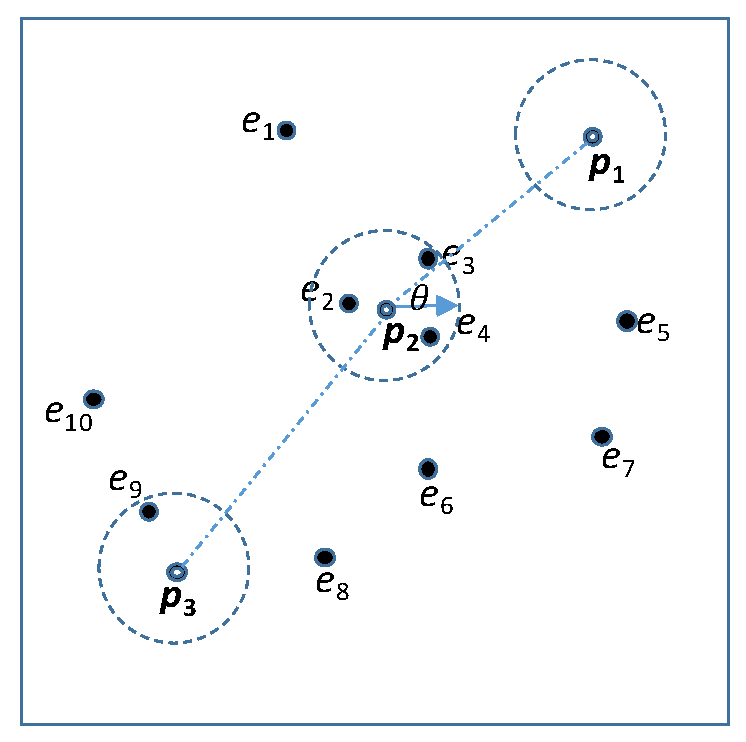
\includegraphics[width=2.7in]{Fig/chapter3/joinmap.eps}	
	}
	\subfigure[]{
		\label{fig:gridindex}
		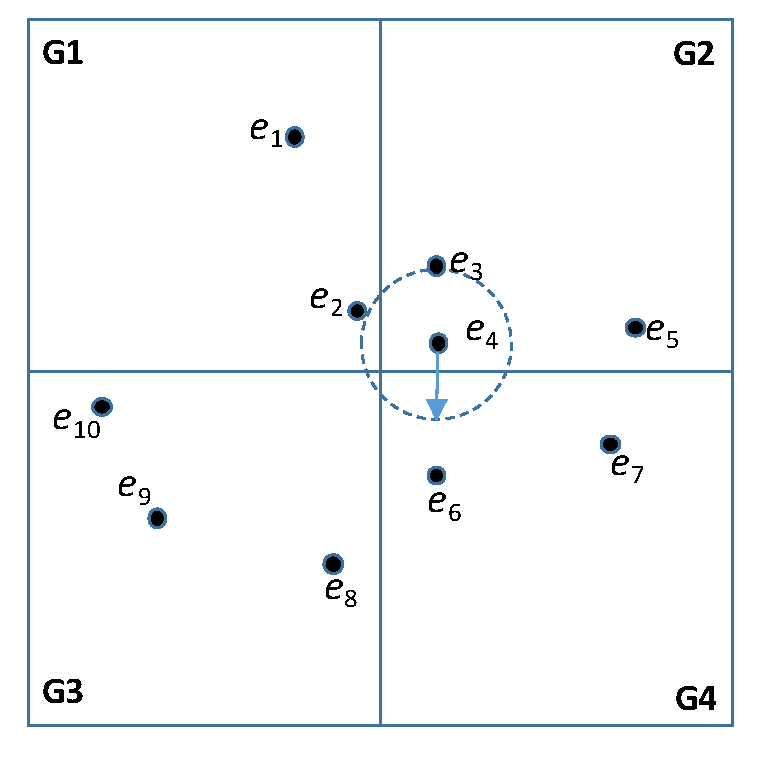
\includegraphics[width=2.7in]{Fig/chapter3/quadtree.eps}
	}
	\subfigure[]{
		\label{fig:globaljoin}
		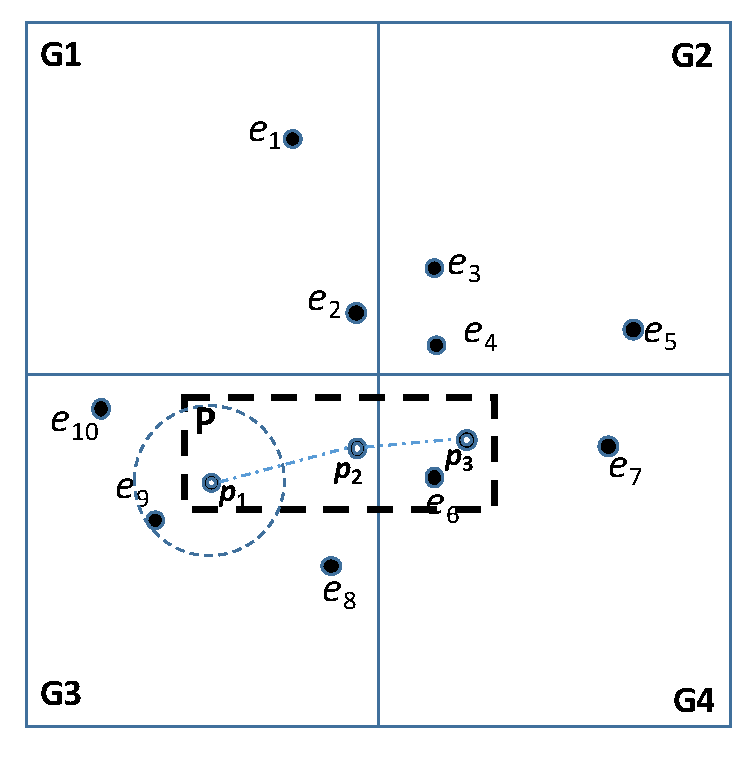
\includegraphics[width=2.7in]{Fig/chapter3/globaljoin.eps}
	}
	\caption{Join查询示例}
	\label{fig:joinprepare}
	\vspace{-0.5cm}
\end{figure}
轨迹的join查询被广泛应用在社交网络和推荐系统中。一个典型的查询应用就是,给定一个轨迹数据集和一个带语义信息的空间对象集合(如POIs、道路和区域),研究者们将这两个数据集关联起来以得到语义轨迹。这样的一个查询可表示为\textbf{Join($IndexTRDD, SP,\epsilon$)},其中 $IndexTRDD$代表轨迹数据,$SP$ 代表空间对象数据集,$\epsilon$ 是查询的空间约束。这个查询将轨迹中的点$p$映射到$SP$中距离最近的点$e$上,且需满足$p$到$e$的距离需小于$\epsilon$。如果点$p$找不到满足条件的映射点,则会将其忽略。图\ref{fig:joinprepare}给出了查询示例,给定查询轨迹$< p_{1}, p_{2}, p_{3}>$ 和由10个点对象构成的空间对象集合(由$e_{1} $ 到 $e_{10}$表示)。根据查询,$p_{1}$ 不会被映射到任何点上, $p_{2}$会被映射到 $e_{2}$ 上,因为 $e_{2}$是$\epsilon$ 范围内最近的点,  $p_{3}$ 将会被映射到 $e_{9}$ 上。

由于轨迹数据集和空间数据集都比较大,暴力查找开销较高。为此,我们需要对$SP$数据集进行预处理。由于整个系统空间被划分成了$m*m$个格子,我们首先对$SP$数据集统计每个格子里点的个数。假设$SP$将被划分成$S$个分区(每个分区对应一个网格,且$S$值由$SP$和分区大小约束两方面决定)。然后,我们构建四叉树或R树来构建索引管理这些格子,使得最终索引树的叶子节点为$S$个。接着,用构建好的树索引划分$SP$得到一个 PairRDD,PairRDD的每个元素的value值为对应的空间点,key值为与该点$\epsilon$范围相交的网格标识。由于点的$\epsilon$范围可能与多个网格相交,因此一个点可能会形成多个键值对。
Fig. \ref{fig:gridindex}介绍了当使用四叉树来划分$SP$时的案例。在该图中,点$e_{4}$ 被映射成4个键值对$<G1,e_{4}>, <G2, e_{4}>, <G3, e_{4}>, <G4, e_{4}>$。最后,我们对这样的PairRDD中键相同的元组看作为一个分区,并对该分区内部空间点构建局部索引。这样$SP$就被转换成具有局部和全局两层索引。完成以上对空间数据集的预处理后,我们设计了如下join查询算法,该算法包含三个主要步骤:全局join,局部join和合并。下面将对这三个部分进行详细介绍。

\textbf{全局 join.} 在该阶段,根据$IndexTRDD$和$SP$的全局索引,将两者有交集的分区形成分区对。如图\ref{fig:globaljoin}所示,带有虚线的方框$P$代表了$IndexTRDD$的一个分区的包围矩形。$P$跟$SP$数据集的$G3$ 和 $G4$相交,因此会形成两个新的数据分区$\langle P, G3\rangle$和$\langle P, G4\rangle$。其中$\langle P, G3\rangle$包含了IndexTRDD的$P$分区和$SP$的$G4$分区的数据。
其中由于$G3$和$G4$所代表的分区包含了除自身范围外还有其边界外$\epsilon$范围内的点(图中$e_4$存在于$G3$和$G4$所对应的分区中),所以构成的分区对会包含join查询结果的完备集。因此,我们对两个数据集的全局索引使用传统的空间join算法,得到相交的分区对。最终,将所有分区对的数据整合在一起,形成新的数据集。

\textbf{局部join.}根据上一步得到的结果,对每一个分区内的属于轨迹的那部分数据,逐步遍历每条轨迹,并对每个点从$SP$部分的索引中找出满足$\epsilon$ 约束的最近邻点。若每个轨迹点找到满足条件的点,则将原始轨迹的位置信息,替换为对应匹配点的信息。若找不到满足条件的点,则忽略该轨迹点。局部join产生的数据即为映射后的轨迹数据,只是将原来的位置信息维度替换为空间数据的标识。
由于某个空间点会存在多个分区中,因此局部匹配后的结果会出现对一个轨迹

 \textbf{合并.}由于$IndexTRDD$的一个分区会与$SP$的多个分区相交,所以存在着某个轨迹点在一个$SP$分区中没有匹配点,但在另一个$SP$分区中有匹配点的情况。如图 \ref{fig:globaljoin}中, $<p_{1}, p_{2}, p_{3}>$ 是一段位于分区 $P$中的片段。当$P$ 和 $G4$产生分区对时,$p_{1}$将不会被匹配到任何点,但是当$P$ 和$G3$构成的分区对时, $p_{1}$会被匹配到$e_{9}$上。因此,在该阶段,我们需要对局部join的结果进行合并以形成最终的结果集。


\section{实验分析}\label{sec-c3-exp}

\subsection{实验设置}
\begin{table}[t]
	\centering  
	\renewcommand\arraystretch{1.2}
	\begin{tabular}{|c|c|c|c|} 
		\hline
		数据集 & 时间 & 记录数 & 大小(Gb)  \\ \hline
		真实数据集 & 2013.10.1-12.31 & 约250万 & 190  \\ \hline
		人工数据集 & 2013.10.1-12.31& 约 1.8亿 & 1400\\ \hline
	\end{tabular}
	\caption{TrajSpark数据集描述}
	\label{table:SystemData}
\end{table}
在本章节我们将验证系统的性能。所有的实验是在由12个节点构建的分布式集群上实现。每个节点包含一个8核Intel E5335 2.0GHz处理器和16G内存,每个节点的操作系统为Ubuntu 12.0.4,并运行着Spark 1.5.2。Spark集群以standalone模式部署。



我们使用了两个轨迹数据集来验证系统的性能\cite{TrajSpark},包含一个真实轨迹数据集合一个人工合成的轨迹数据集。数据集描述如
表\ref{table:SystemData}所示,这两个数据集为13,007量北京出租车在3个月内(2013年10月至12月)产生的轨迹数据。每条记录包含了如下信息:车的标识、采集时间、经度、纬度、速度和角度等其他描述信息。真实数据集含约250万条轨迹日志记录,数据量为190Gb。为了更好的演示TrajSpark系统的可扩展性,我们根据真实数据集生成了人工数据集。生成方法为将出租车在运行过程中的点通过差值法增加数据使得每5秒种有一个点产生。生成的人工数据集含约1.8亿条记录,数据量为1.4Tb。需要指出的是,真实数据集可以完全被加载入系统内存,而人工数据集无法被完全加载。

在TrajSpark系统中我们将整个北京空间划分成$1,000*1,000$个细格子,使得每个格子覆盖的范围为180m*180m。我们将TrajSpark跟最新的两个空间数据管理系统GeoSpark和Simba从查询延迟和可扩展性两方面进行对比分析。其中延时指标使用10个查询的平均时间进行计算。


\subsection{实验结果及分析}

	\begin{figure}[t]
	\centering
	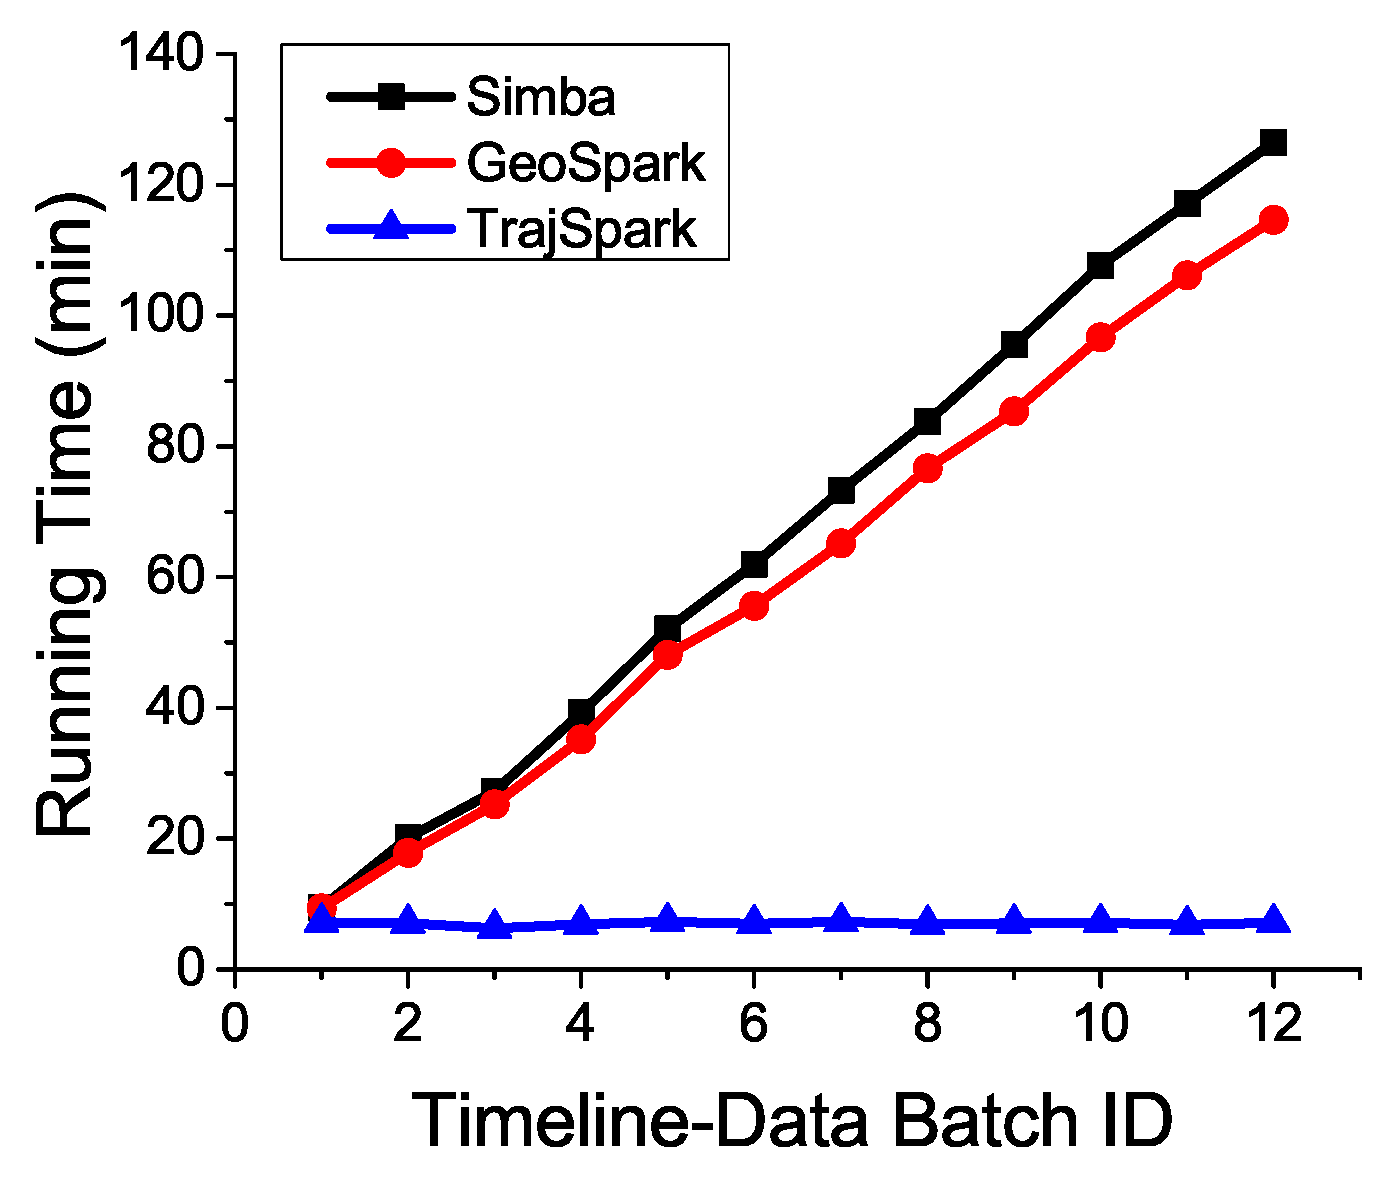
\includegraphics[width=3in]{Fig/chapter3/loadfinal.eps}
	\caption{数据加载开销}
	\label{fig:loadtime}
\end{figure}

首先,我们研究了系统加载数据的时间开销。图\ref{fig:loadtime}介绍了当所有系统随着数据不断导入到系统,系统更新一批数据的时间开销,其中每一批数据的大小为32Gb。
从图中可以发现GeoSpark和Simba都随着已转入数据量的增加导致新来的数据加载时间呈线性增加。这是由于这两个系统会将已有数据和新来的数据结合起来统一考虑,然后将两者作为整体重新划分。划分的过程会导致数据的洗牌,占用较多的网络通信和磁盘I/O开销。而TrajSpark由于只需对新来的数据进行数据划分,然后将划分后的分区信息汇总入全局索引中。因此,划分开销并不会随着数据的增加而发生较大变化。综上所述,TrajSpark具有较好的数据可扩展特性。


 \begin{figure}[t]
	\centering
	\subfigure[RDD存储开销]{
		\label{fig:local}
		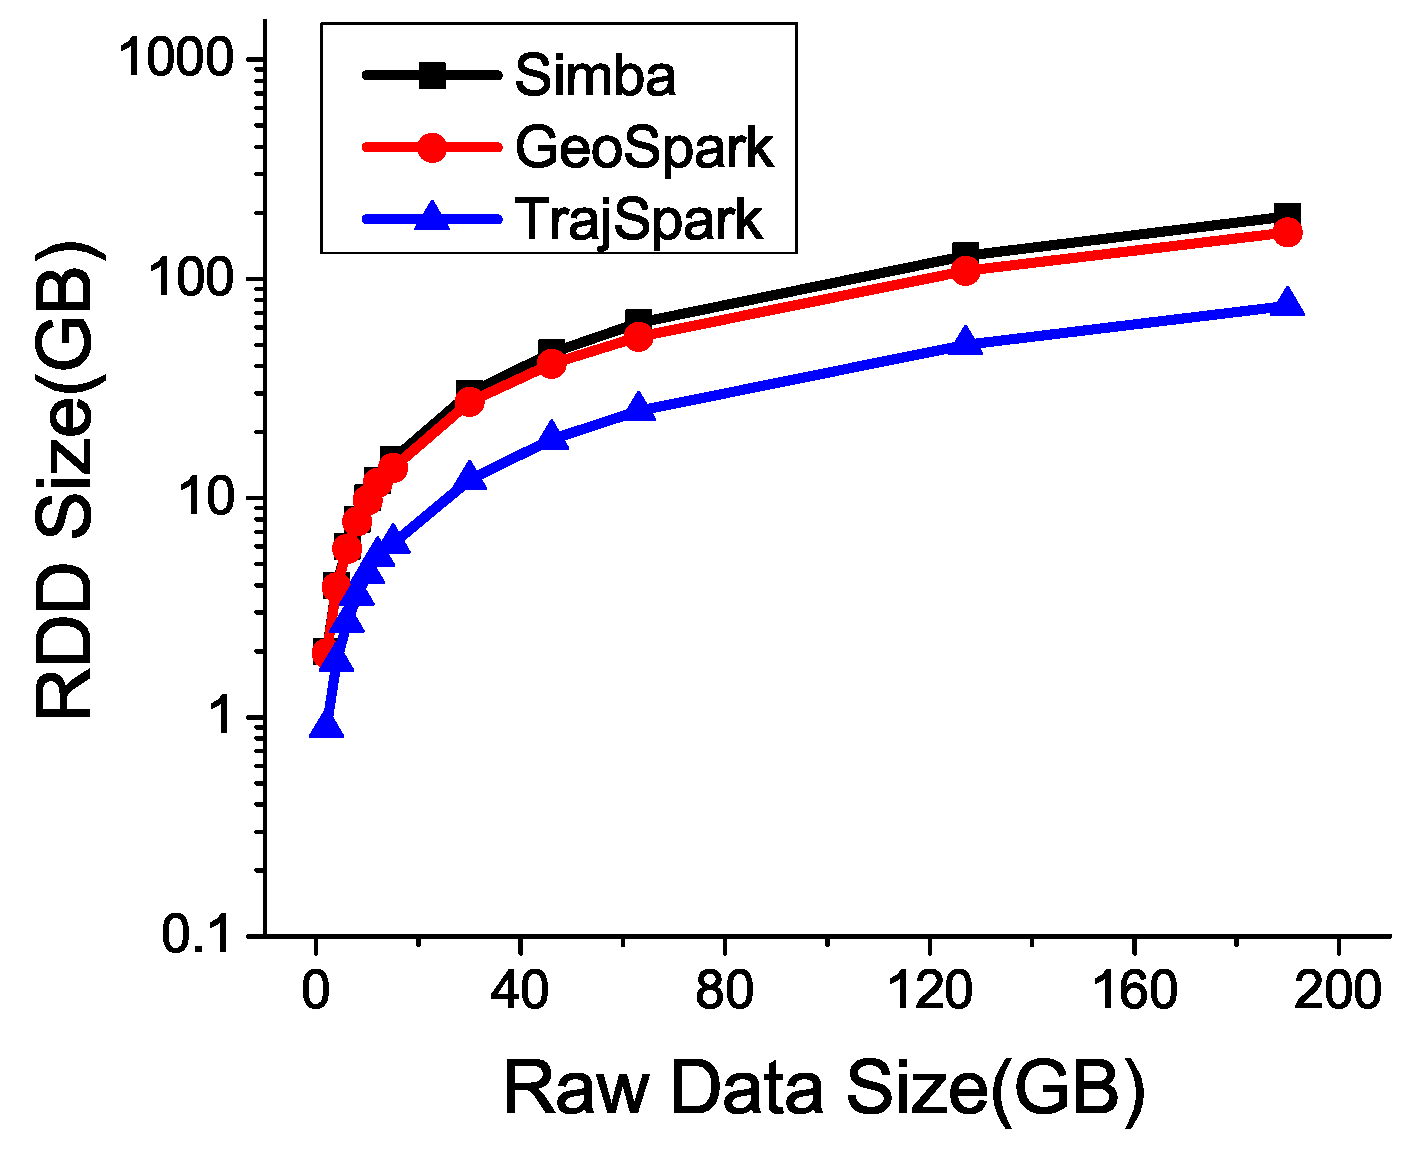
\includegraphics[width=2.7in]{Fig/chapter3/LI.eps}		
	}
	\subfigure[全局索引存储开销]{
		\label{fig:global}
		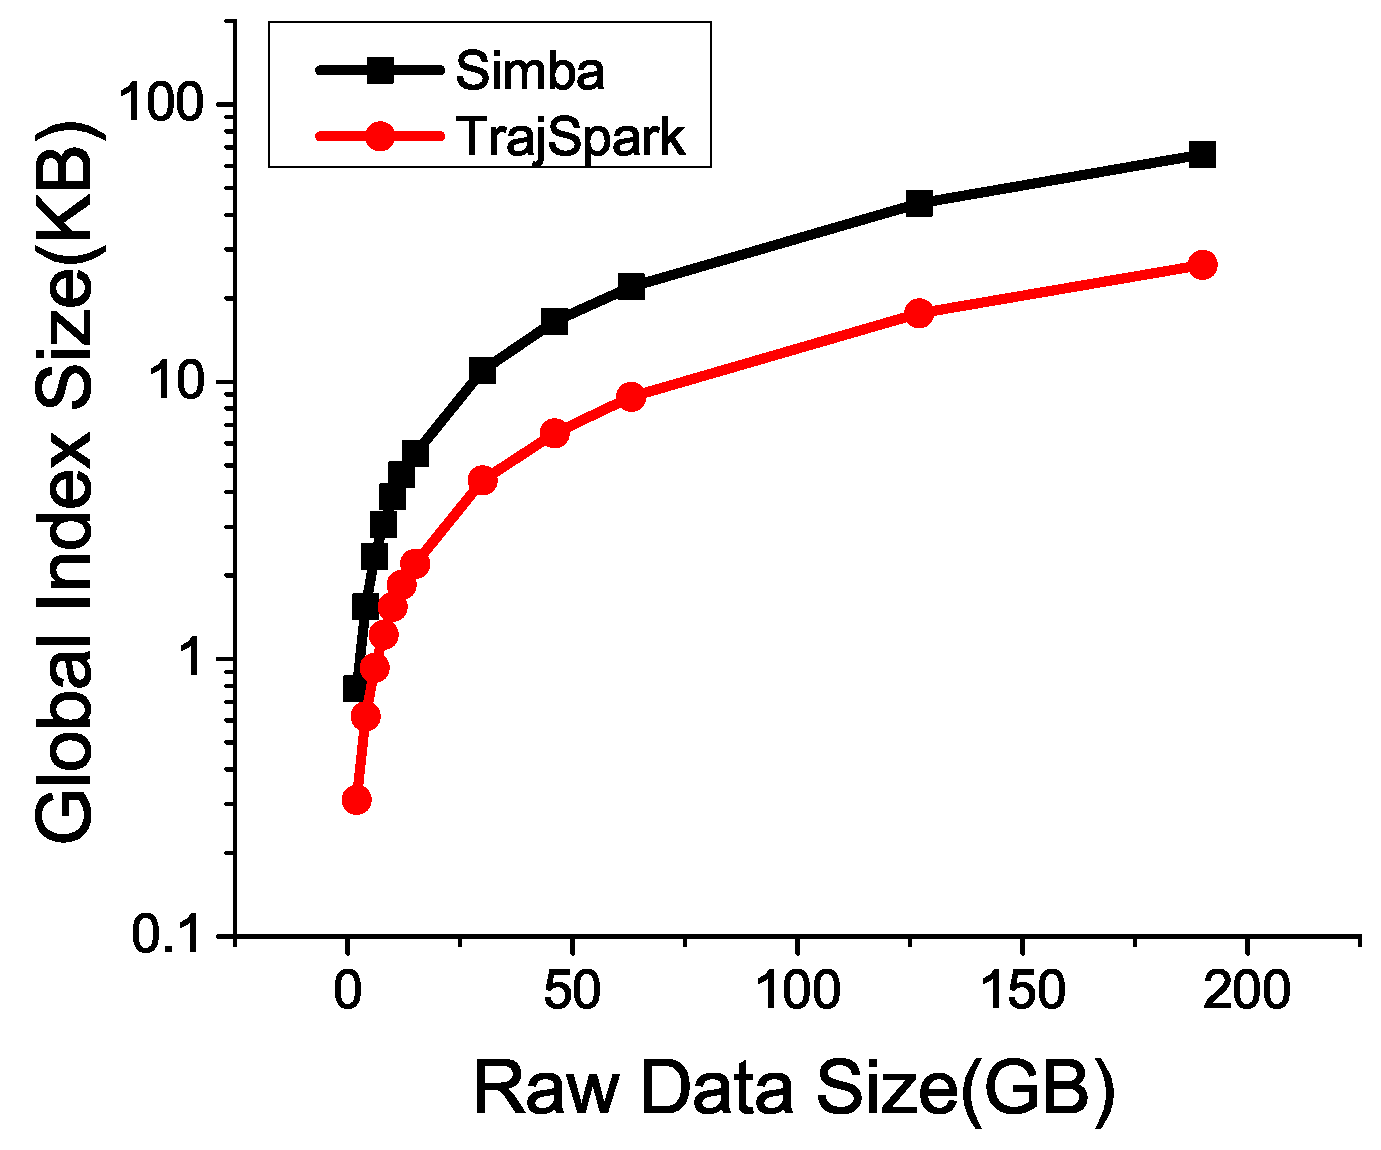
\includegraphics[width=2.7in]{Fig/chapter3/GI.eps}
	}
	\caption{数据存储开销}
	\label{fig:storage}
\end{figure}

接着,我们研究了从IndexTRDD和全局索引两部分的存储开销随数据量的变化情况。图\ref{fig:storage}展示了3个系统当不同数据量级的轨迹数据加载后,数据存储和全局索引两者存储开销的变化情况。其中图\ref{fig:local}显示当数据加载入TrajSpark系统后,所消耗的存储开销最低。而当加载入Simba和GeoSpark后消耗的存储开销是TrajSpark的2-3倍。这是因为TrajSpark会将原始轨迹数据按列存储形式存放并进行压缩,而后两者直接存放原始数据,数据冗余较多。图\ref{fig:global}介绍了3个系统的全局索引存储开销。从图中可以发现这一开销在三个系统内部均较少(数量级为Kb),因而都可以轻松存放到内存中。其中TrajSpark系统的全局索引开销最少(约是Simba的1/3),这是因为其数据压缩后,每个分区能放入跟多的数据,从而导致分区数较少。而全局索引是构建在分区之上的,所以TrajSpark会消耗更少的内存来存放全局索引。



然后,我们验证了TrajSpark在基于给定对象的查询在不同数据量下的效果。图\ref{fig:ID-based} 展示了查询性能。从该图中我们可以发现TrajSpark比Simba快了一个数量级,且比GeoSpark快了两个数量级。这是由于GeoSpark需要遍历整个数据集,所以其效果最慢。而Simba虽然能通过全局索引剪枝掉不相关的数据分区,但它仍然需要遍历每个分区内部的所有数据。相比较而言,TrajSpark既使用了全局索引剪枝分区,又在每个分区内使用局部哈希索引进行随机访问。
需要注意的是,这些系统在真实数据集上的延时比人工数据集下的低。这是由于内存容量可以存放大部分真实数据集,而只能转载的下少部分人工数据集。所以人工数据集下的查询会有额外的I/O开销。尽管如此,这些系统在人工数据集下仍取得较好的结果。这是由于以下两点原因:(1)我们将数据以``MEM\_AND\_DISK\_SER''形式存放,经常被访问的数据会被存放到内存中;(2)使用全局索引,能避免很多I/O开销。
\begin{figure}[t]
	\centering
	\subfigure[真实数据集]{  
		\label{fig:RealID}
		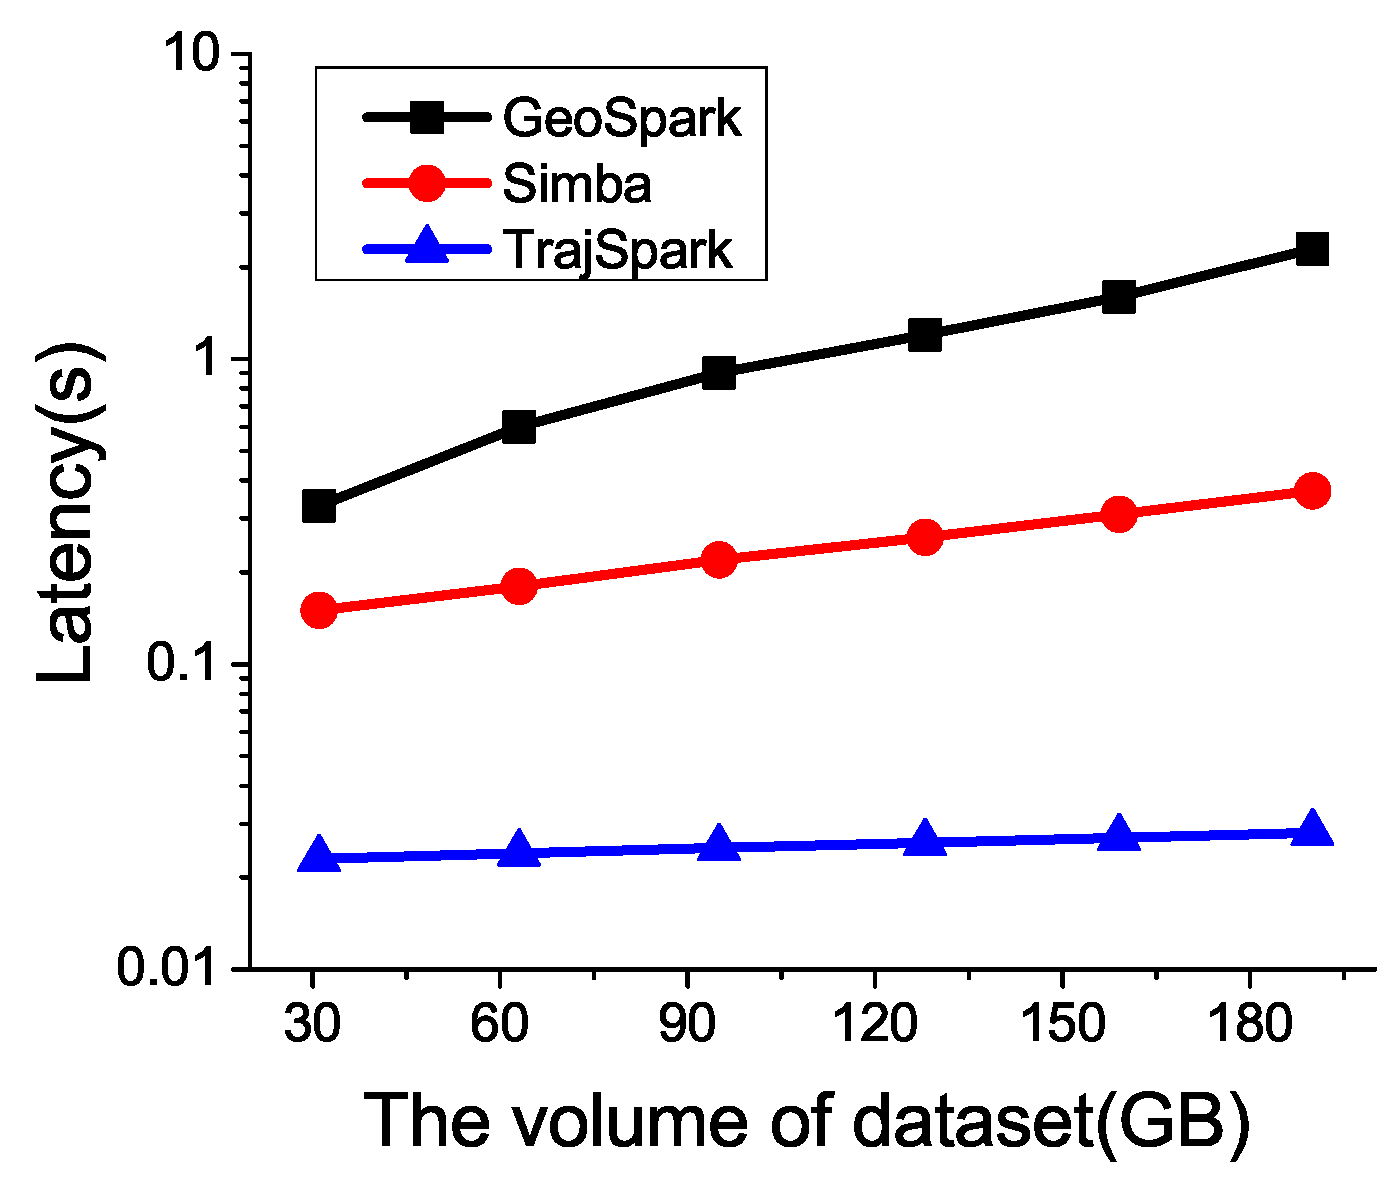
\includegraphics[width=2.7in]{Fig/chapter3/idS.eps}	
	}
	\subfigure[人工数据集]{
		\label{fig:synthetic}
		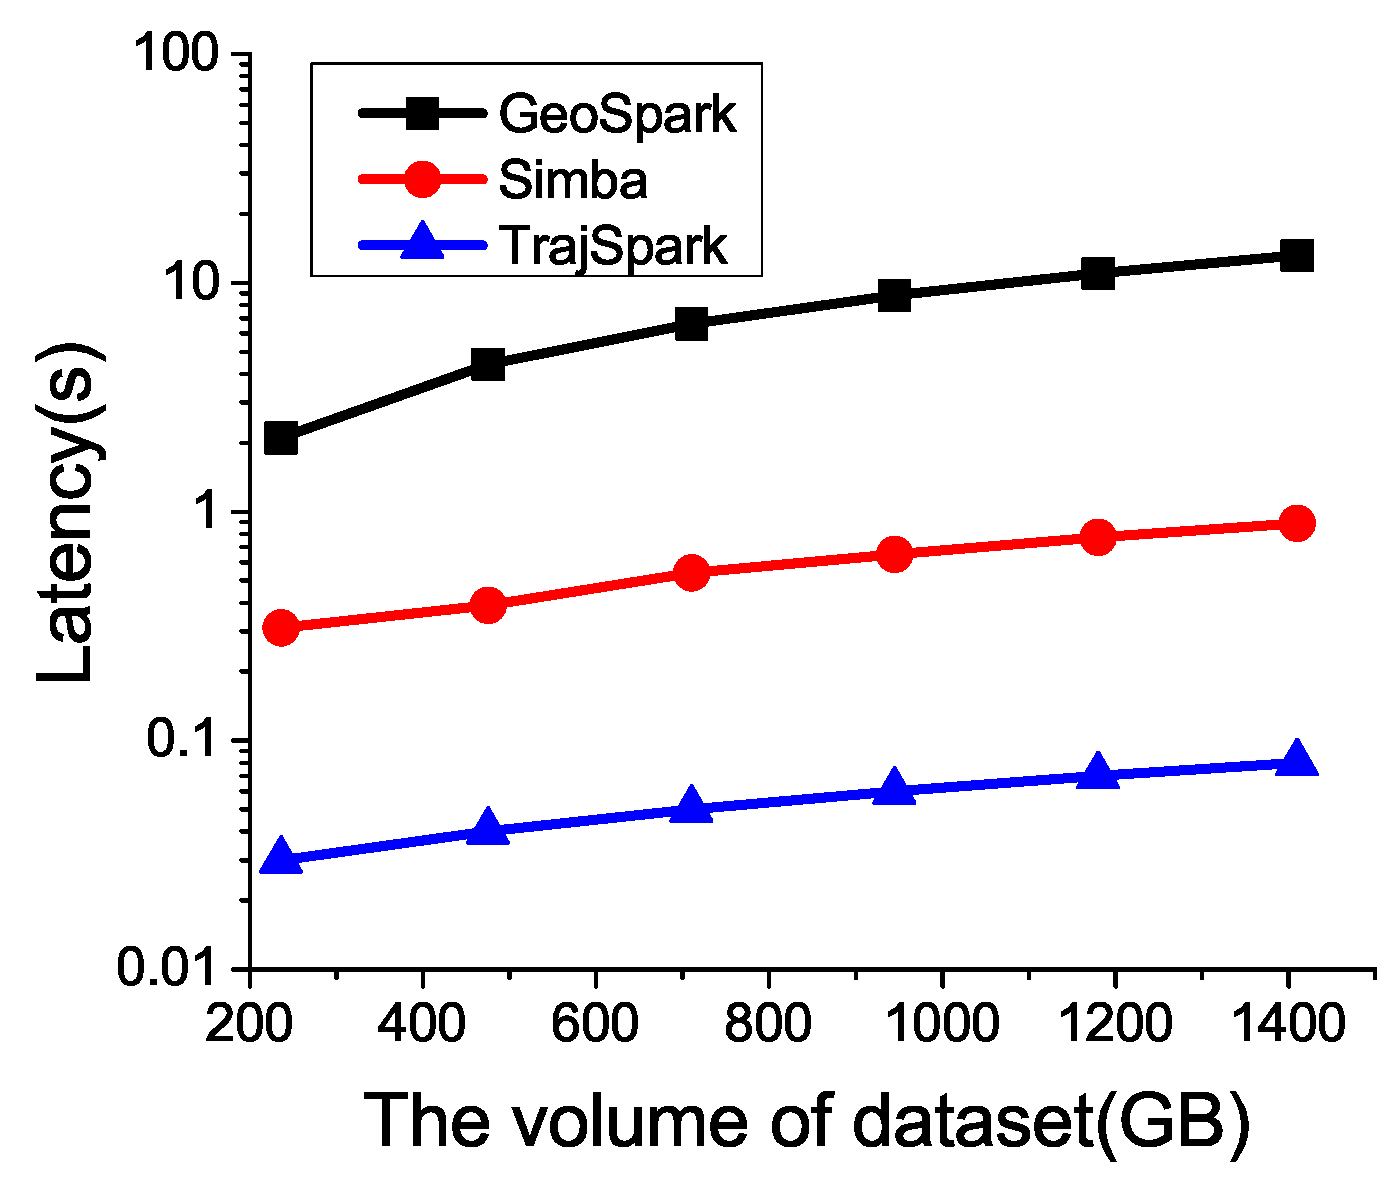
\includegraphics[width=2.7in]{Fig/chapter3/idB.eps}
	}
	\caption{基于给定对象的查询性能}
	\label{fig:ID-based}
\end{figure}

\begin{figure}[t]
	\centering
	\subfigure[真实数据集]{  
		\label{fig:RealST}
		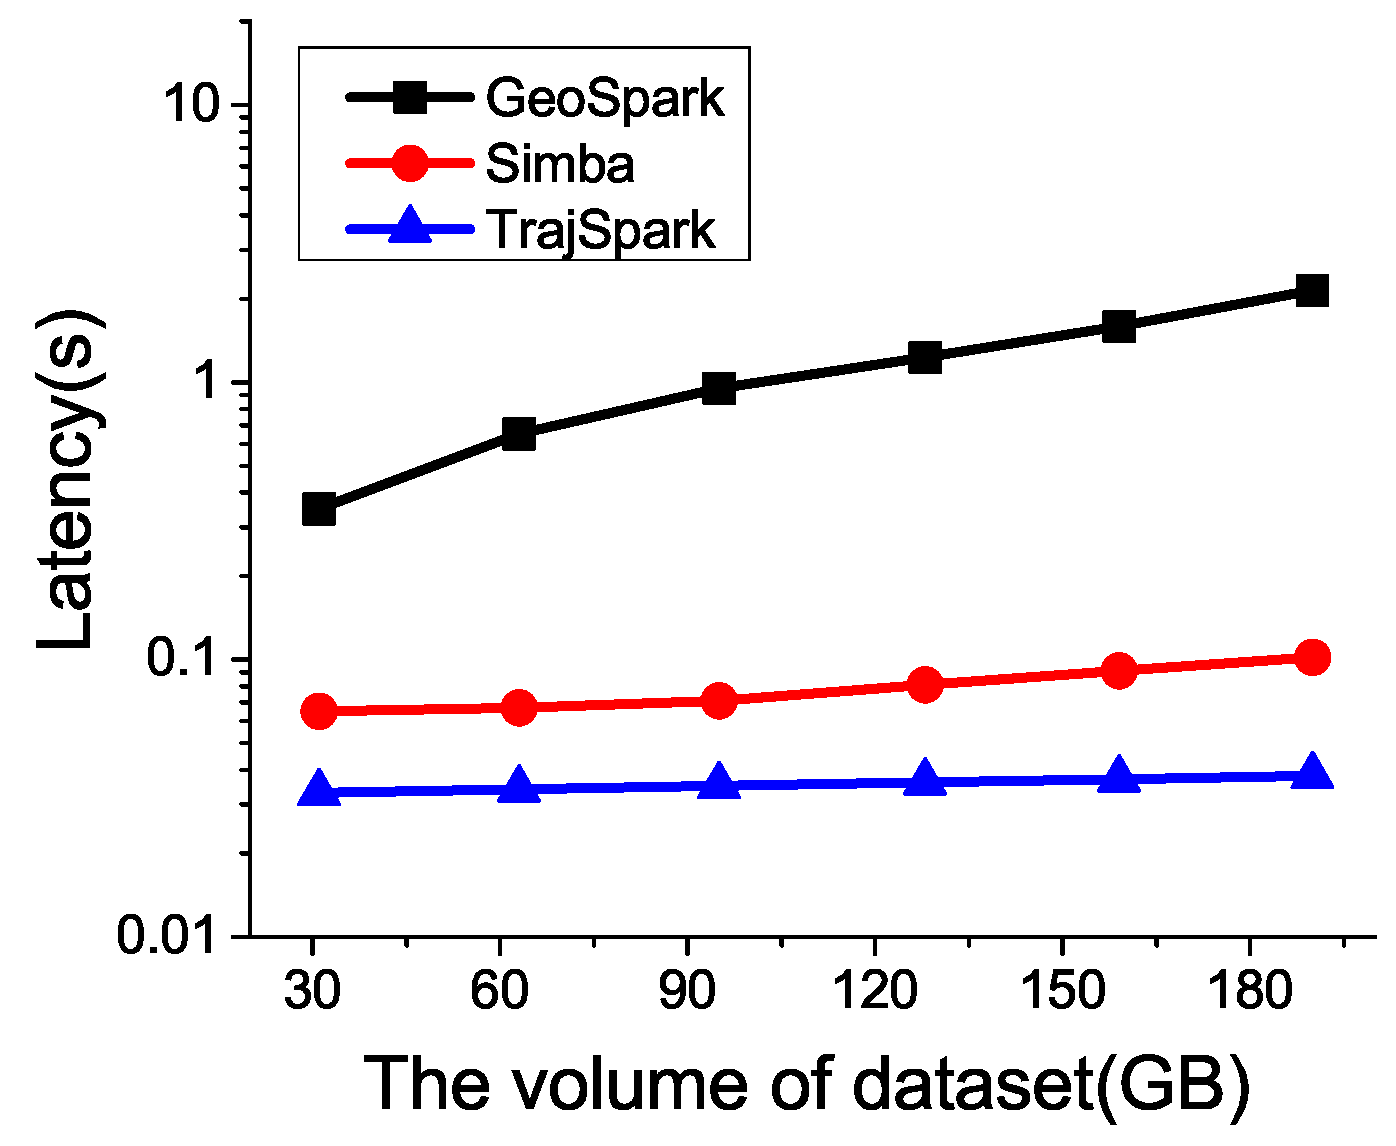
\includegraphics[width=2.7in]{Fig/chapter3/RangeS.eps}	
	}
	\subfigure[人工数据集]{
		\label{fig:syntheticST}
		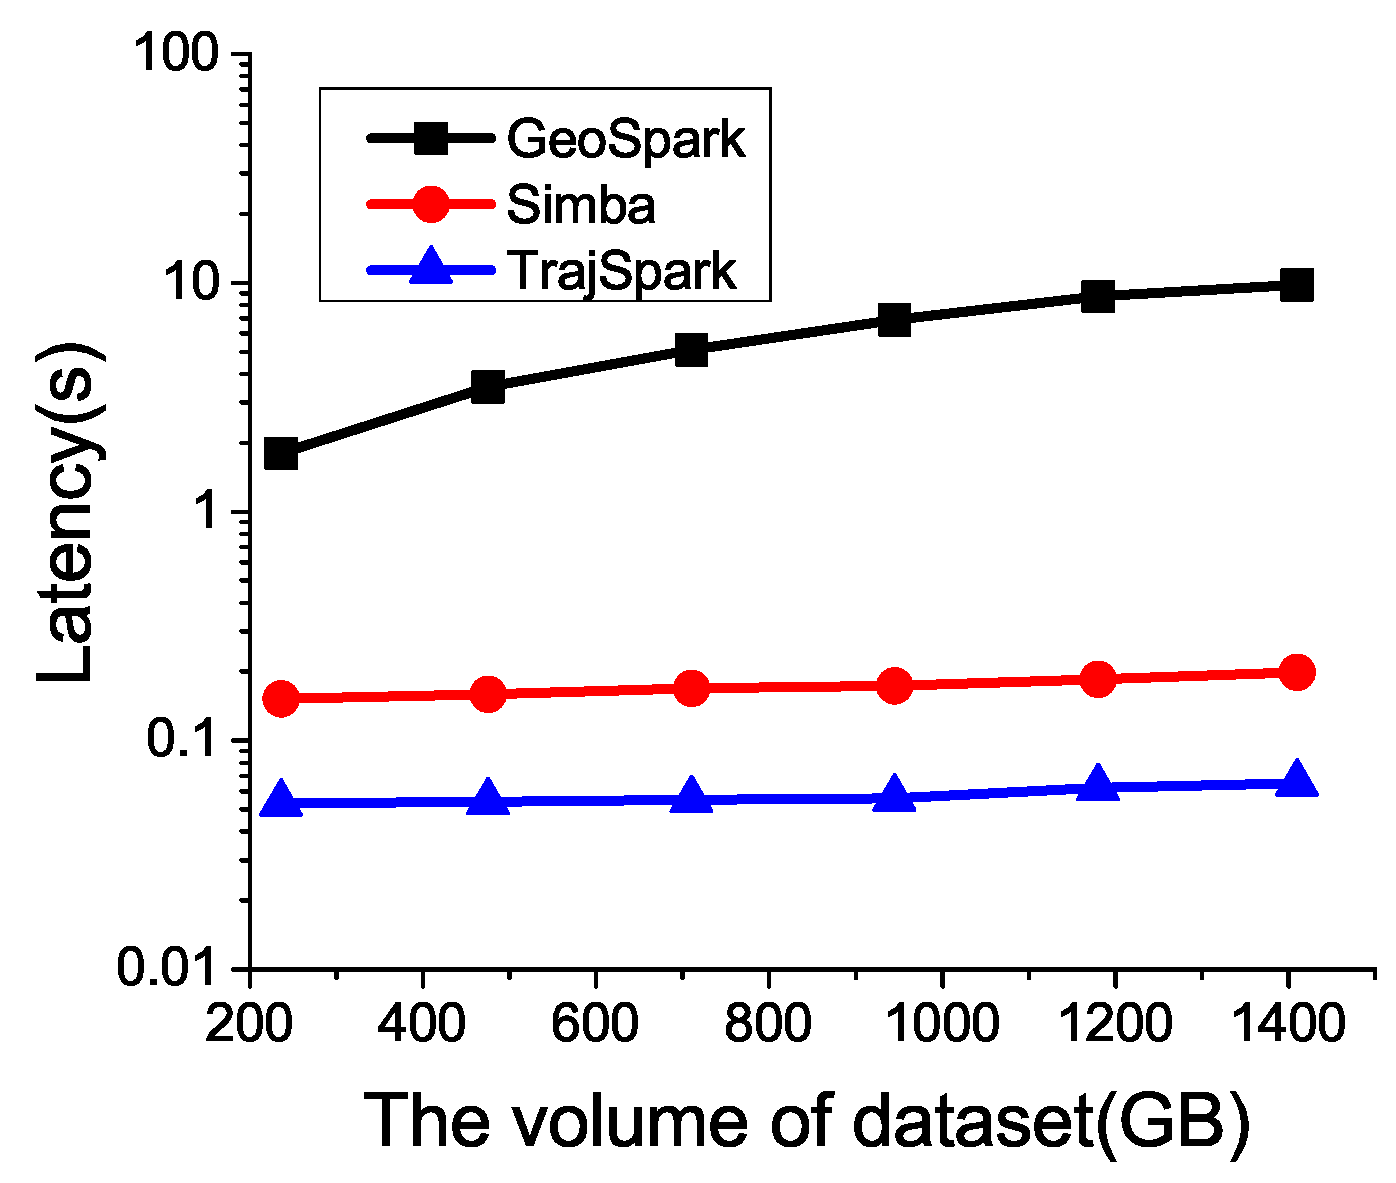
\includegraphics[width=2.7in]{Fig/chapter3/RangeB.eps}
	}\\
	\subfigure[TrajSpark---真实数据集]
	{  \label{fig:RealSPVarious}
		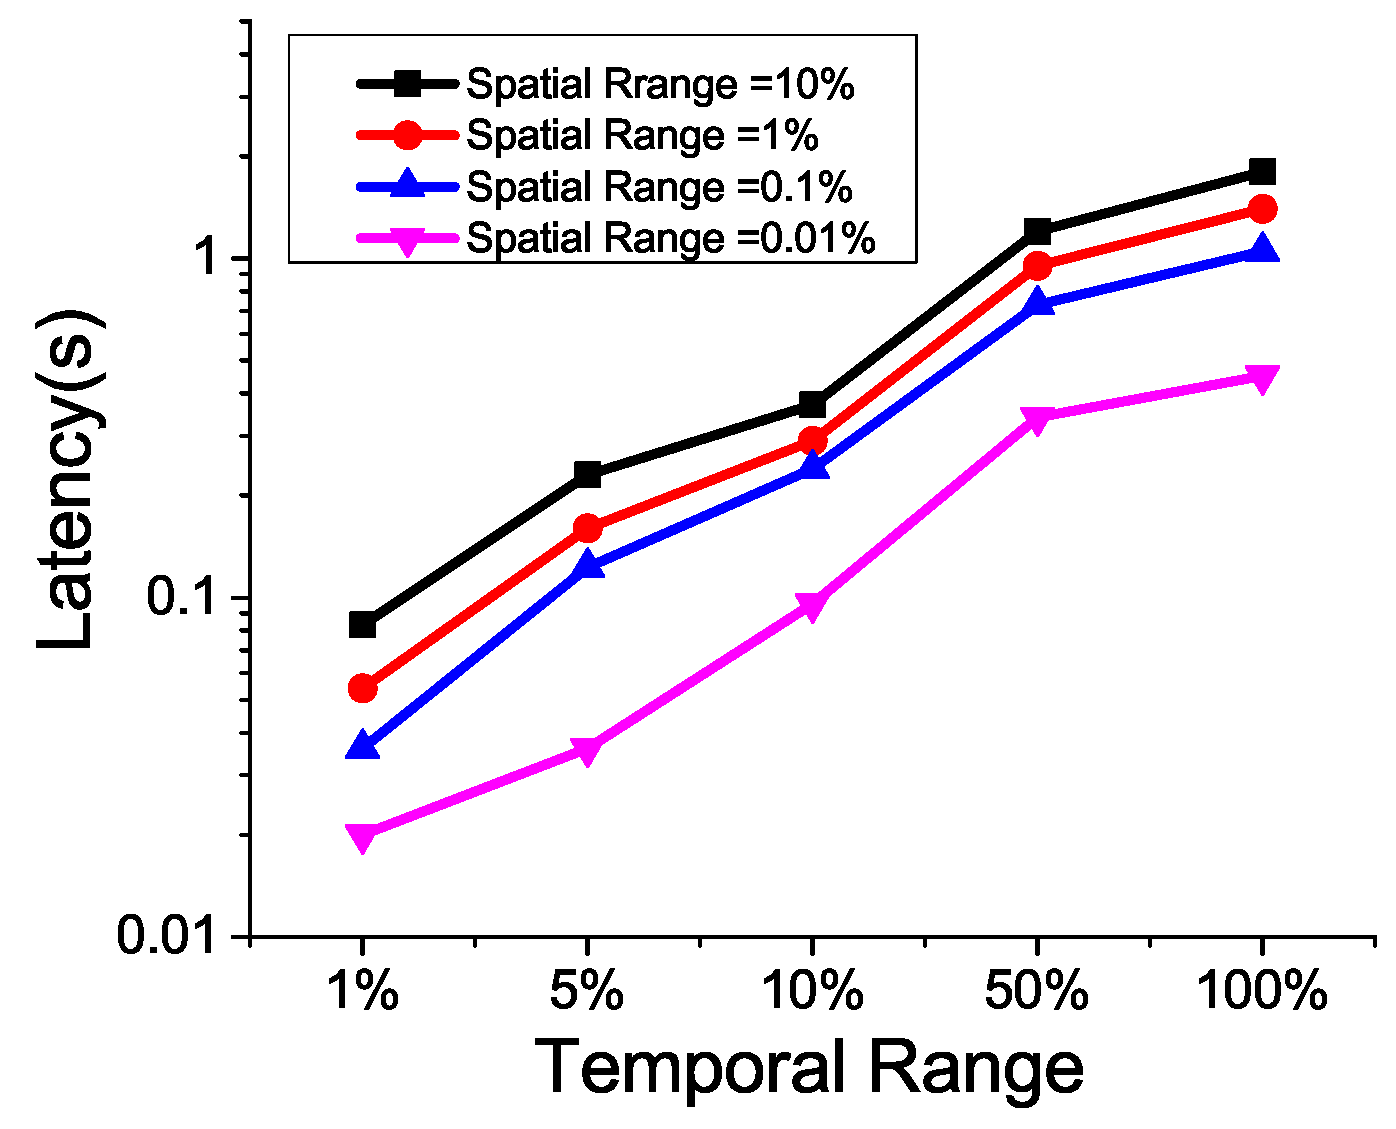
\includegraphics[width=2.7in]{Fig/chapter3/spvSmall.eps}
	}
	\subfigure[TrajSpark---人工数据集]
	{
		\label{fig:GeneratedSPVarious}
		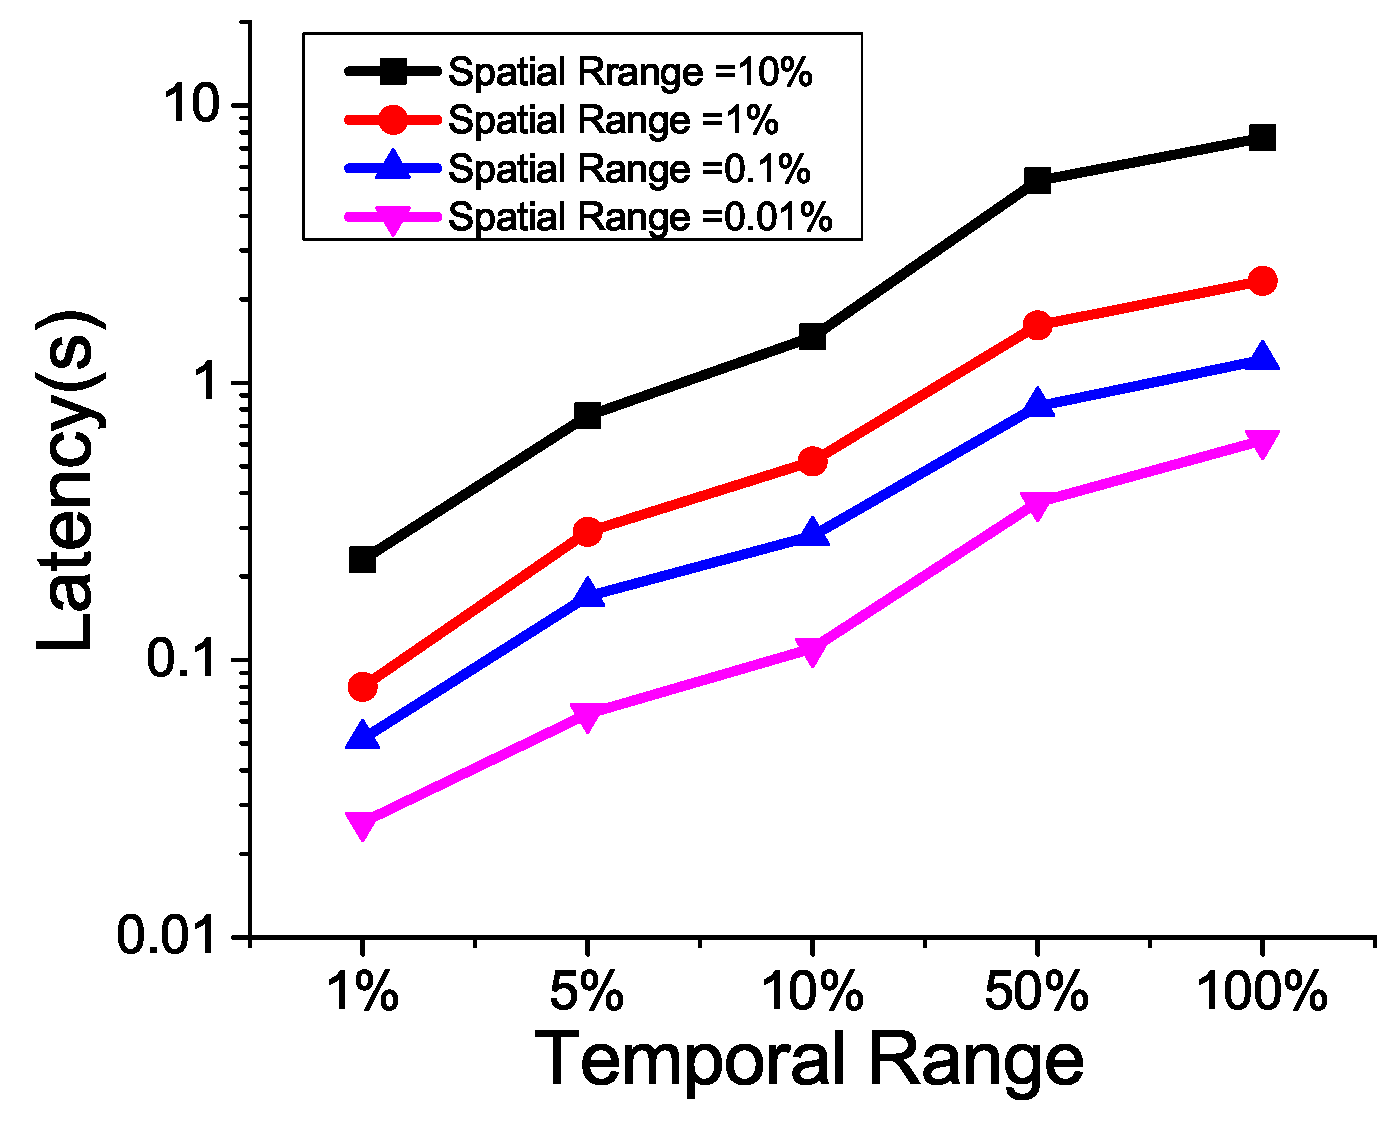
\includegraphics[width=2.7in]{Fig/chapter3/spvBig.eps}
	}
	\caption{时空范围查询性能}
	\label{fig:ST-based}
\end{figure}


\begin{figure}[t]
	\centering
	\subfigure[真实数据集]{  
		\label{fig:knSmallSc}
		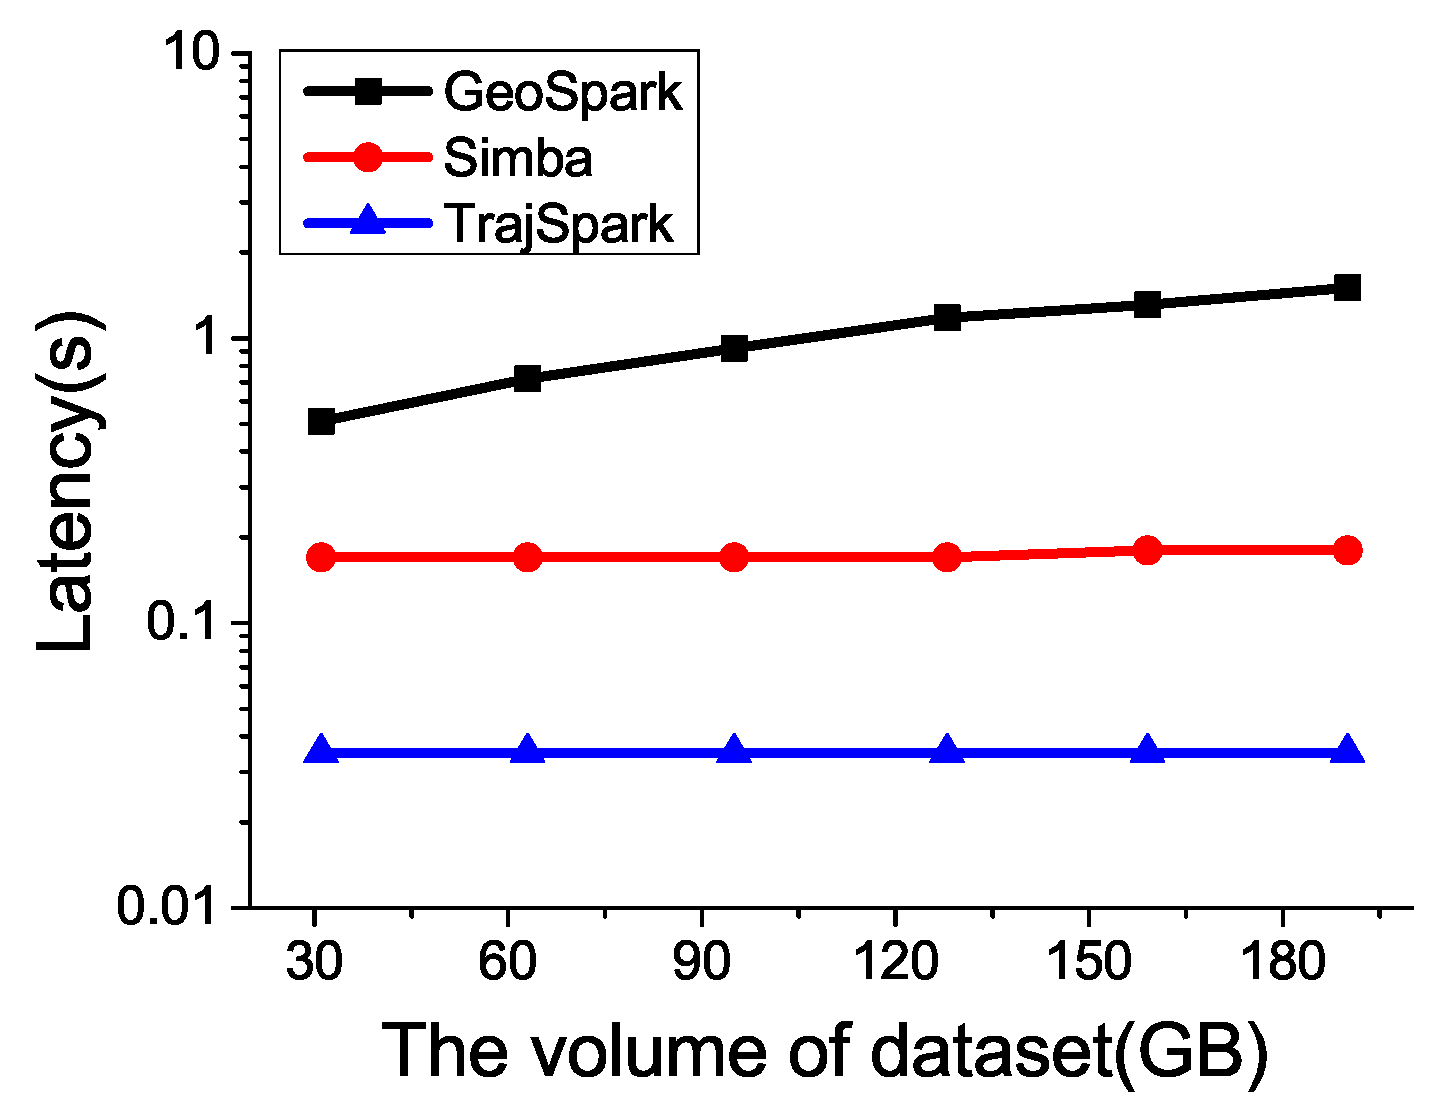
\includegraphics[width=2.7in]{Fig/chapter3/scKNNsmall.eps}	
	}
	\subfigure[人工数据集]{
		\label{fig:knBigSc}
		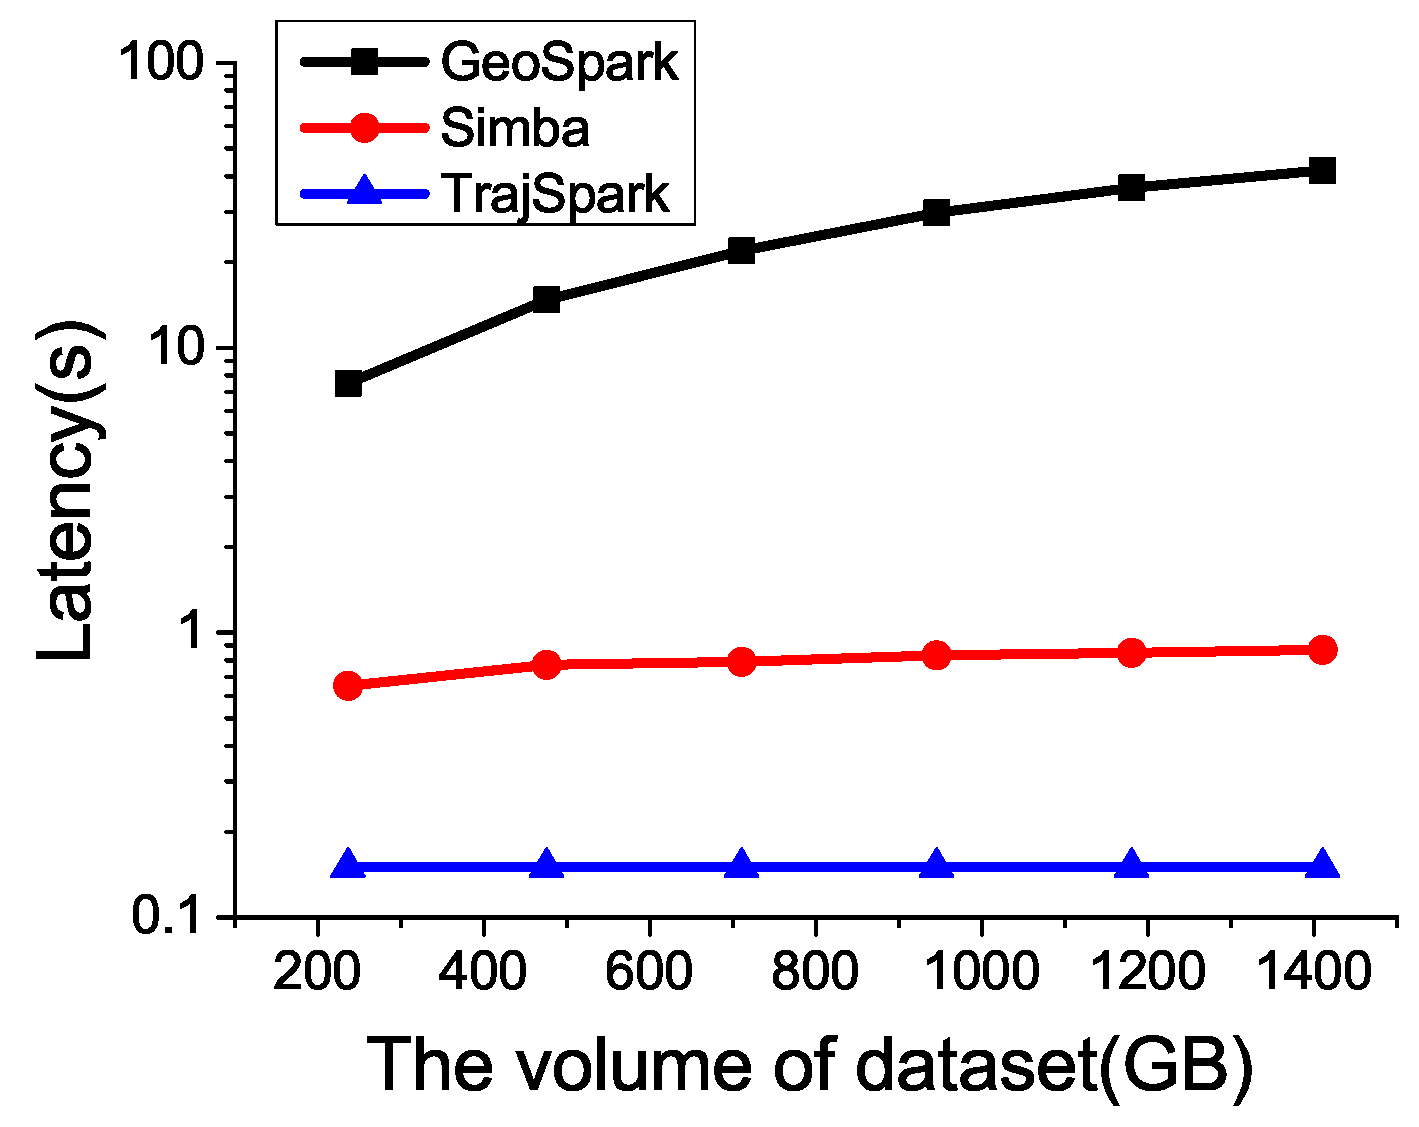
\includegraphics[width=2.7in]{Fig/chapter3/scKNNlarge.eps}
	}\\
	\subfigure[TrajSpark真实数据集]
	{  \label{fig:knSmall}
		\includegraphics[width=2.7in]{Fig/chapter3/knnSmall.eps}
	}
	\subfigure[TrajSpark人工数据集]
	{
		\label{fig:knBig}
		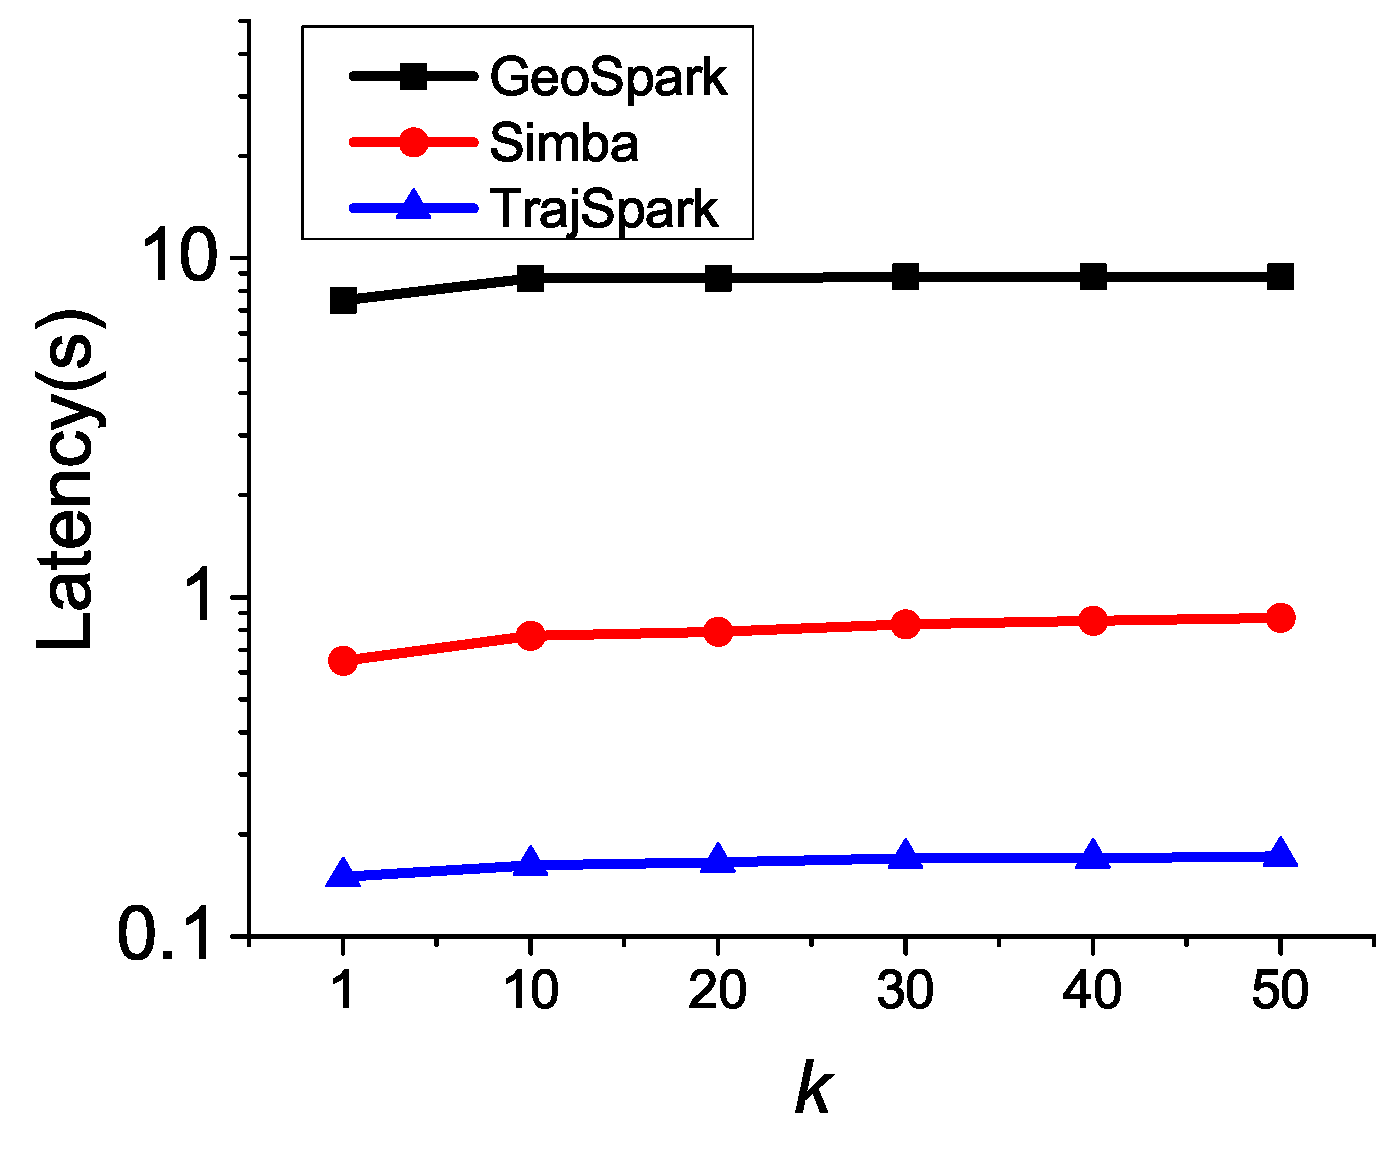
\includegraphics[width=2.7in]{Fig/chapter3/knnLarge.eps}
	}
	\caption{$k$近邻轨迹查询性能}
	\label{fig:knn}
\end{figure}

其次,我们验证了TrajSpark在时空范围下的查询性能。由于数据分布的不均匀性,查询空间范围的选取对查询效率有着较高的影响。为此,我们随机选择了100个包含20*20个方格的区域作为查询的空间约束,选取最近的一周作为当前数据的查询时间约束。查询延时使用100个查询时间的平均值来计算。
实验结果如图\ref{fig:ST-based}所示,其中图\ref{fig:RealST}和\ref{fig:syntheticST}介绍了查询时间随数据量大小的变化情况。我们可以发现,随着数据量的增加,TrajSpark和Simba上的查询效率并没有发生较大变化,这是由于其全局和局部两层索引剪枝的效果。而GeoSpark由于需要遍历数据集,导致随着数据的增加而查询时延逐渐增大。 此外,可以发现 TrajSpark比Simba快了3-5倍,这是由于其可以使用轨迹的MBR和时间范围来快速剪枝轨迹。
此外,我们验证了查询时间随空间和时间约束变化的情况。我们将空间范围选取了整个空间的 $10\%$, $1\%$, 和 $0.1\%$ ,时间范围选取了三个月的后 $100\%$, $50\%$, $10\%$, $5\%$ 和 $1\%$ 。
从图\ref{fig:RealSPVarious}和\ref{fig:GeneratedSPVarious}可以发现随着查询时间和空间范围的增加,查询的时间也随之增加。但增加的方式并不是线性的。比如,当空间范围设置为$0.01\%$时,我们变换时间范围从$1\%$变化 到 $100\%$,空间范围扩大了100倍,但查询时间只延长了30倍。因此,
TrajSpark处理大的时空范围查询仍能取得较好的效果。

再接着,我们验证了TrajSpark处理欧氏距离下$k$近邻查询的性能。
图\ref{fig:knSmallSc} 和\ref{fig:knBigSc} 展示了当 $k$设置为10时,查询时间随数据量大小的变化情况。我们可以发现TrajSpark比GeoSpark快了两个数量级,比Simba快了4-6倍。这是由于TrajSpark和Simba使用全局索引剪枝时空不相关数据分区,而GeoSpark需要遍历数据集的结果。此外TrajSpark由于不需要对同一个移动对象的轨迹点重新排序,因而查询效率更高。这一查询结果与时空范围类似,这是因为$k$近邻查询首先会执行一个迭代的时空范围查询。进一步地,我们将 $k$值从1变化到$50$以查看$k$值对查询效率的影响。从图\ref{fig:knSmall}和\ref{fig:knBig}可以看出$k$值对查询结果影响不大。这是距离较近的轨迹大都放在跟查询轨迹相同的分区内,而每个分区存放的轨迹数远超50个。

 \begin{figure}
	\centering
	\subfigure[]
	{  \label{fig:joinCmp}
		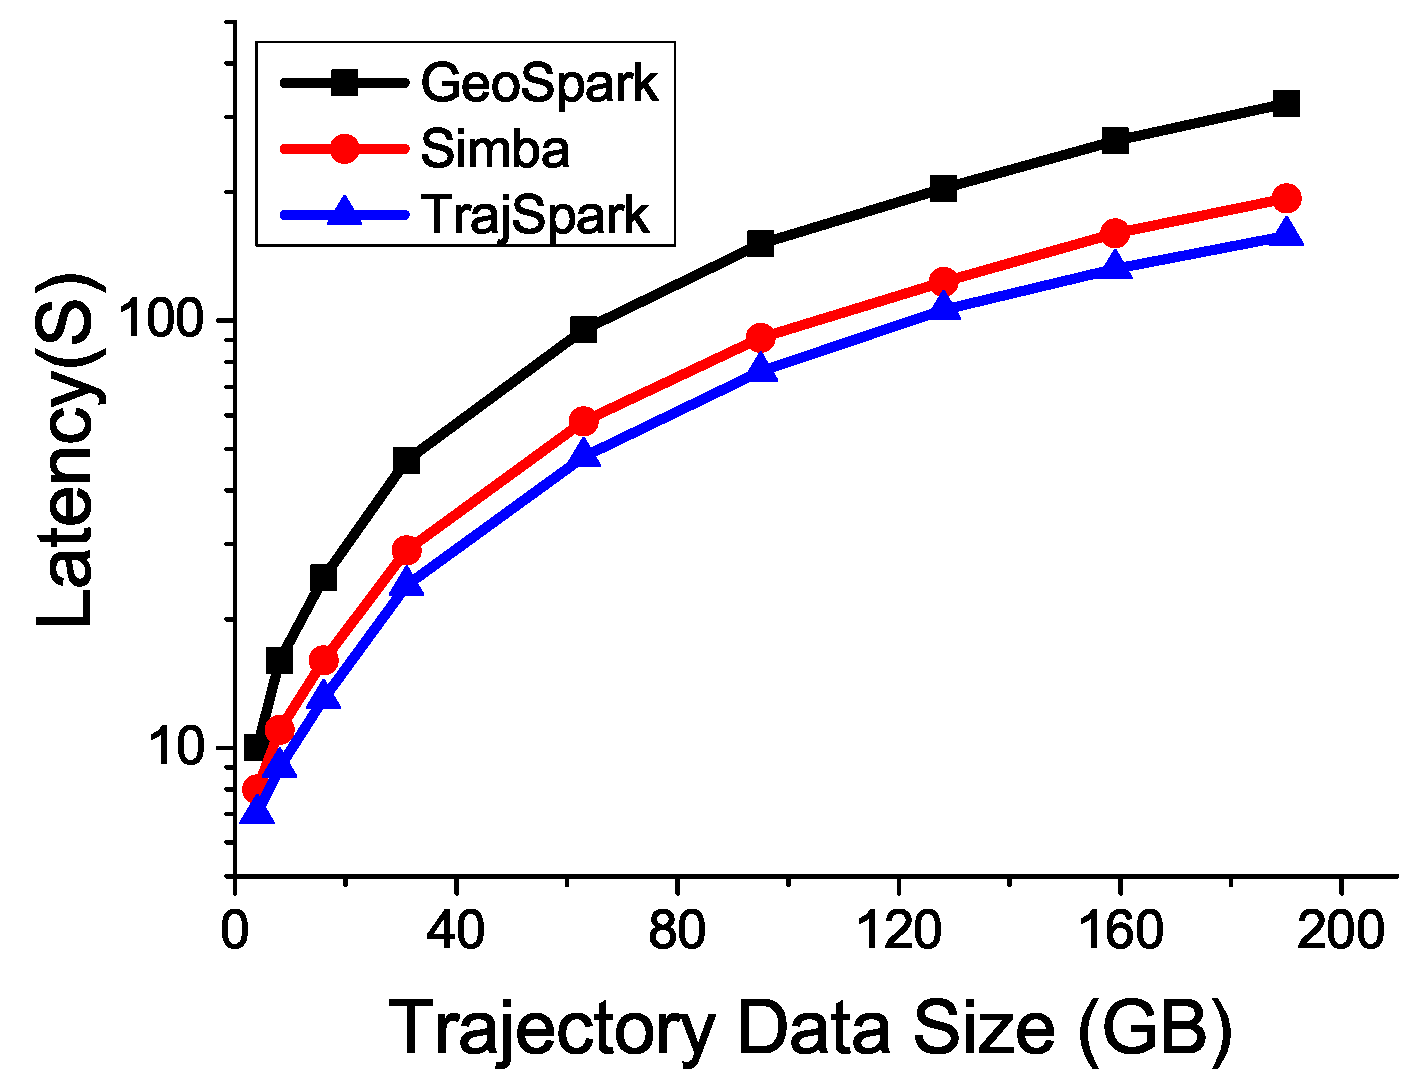
\includegraphics[width=2.7in]{Fig/chapter3/joinCmp.eps}
	}
	%	\hspace{0.005in}
	\subfigure[]
	{
		\label{fig:joinTheta}
		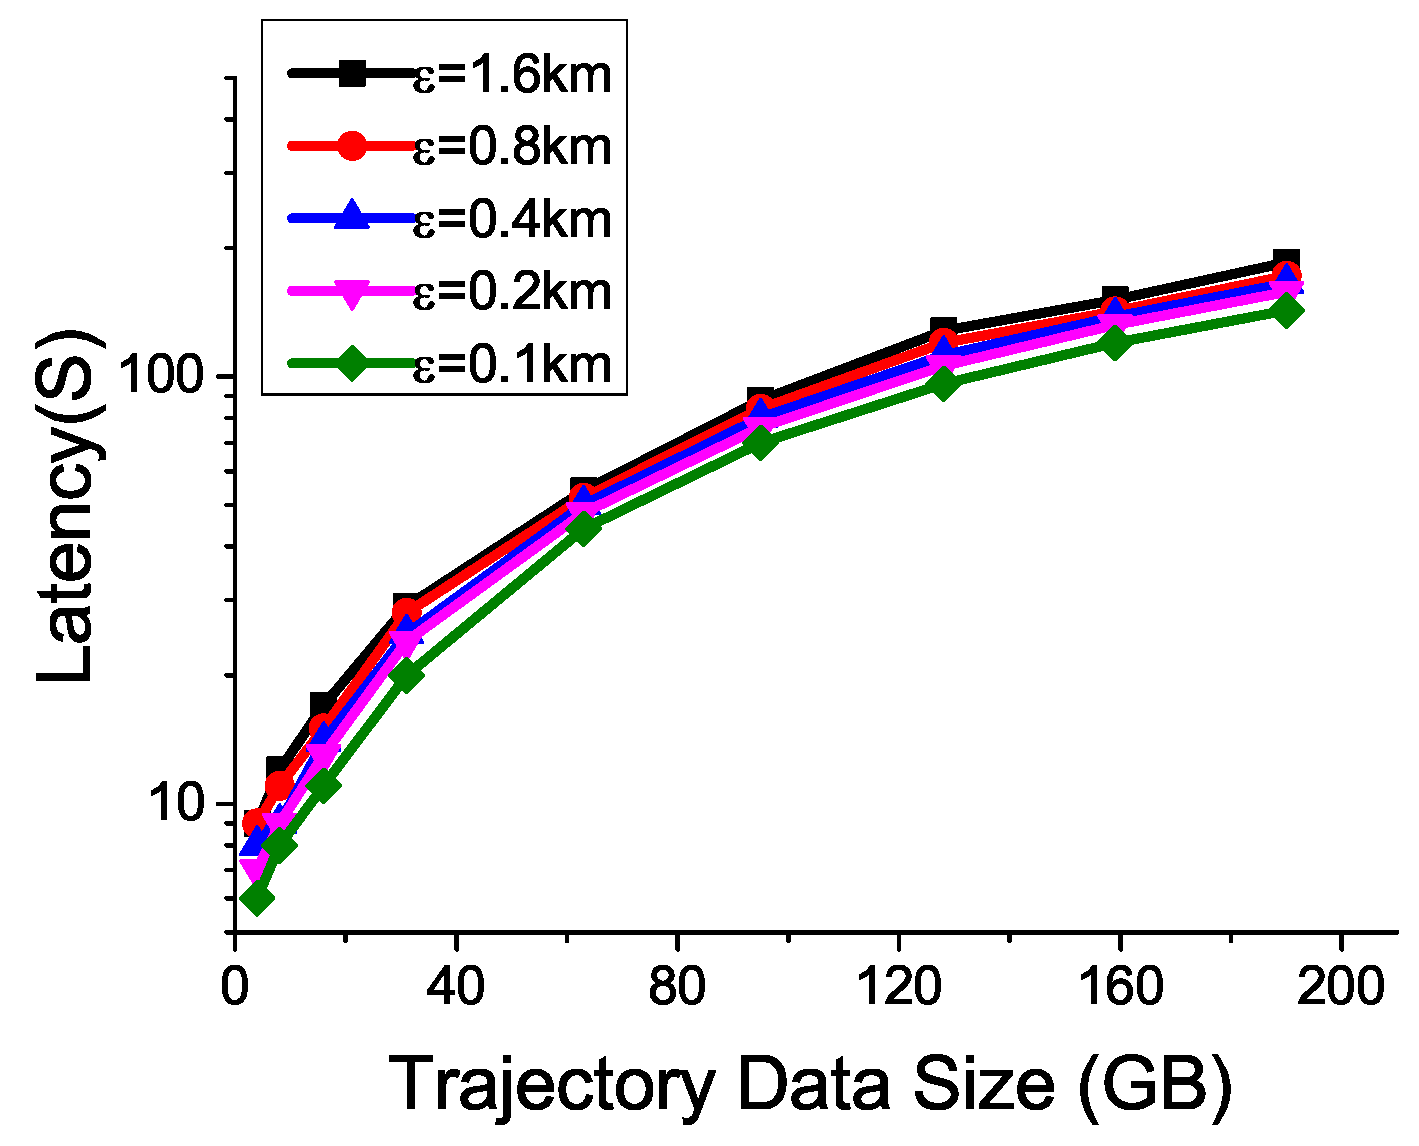
\includegraphics[width=2.7in]{Fig/chapter3/joinTheta.eps}
	}
	\caption{Join查询性能}
	\label{fig:joinExp}
\end{figure}

最后,我们验证了TrajSpark处理join查询的性能。实验所用空间数据集包含两部分数据:北京路网数据结合\cite{ShangZTCY14}和北京POI 数据集合\cite{ShangZTCY14}。其中路网上界集包含148,110  个点 和 196,307条边,而POI数据集包含 273,165 个POI点。
为保持结果简洁,我们只展示了当使用四叉树来索引空间数据的情况(其他索引下结果趋势相同)。Simba实现本文join查询需要结合其自身提供的$k$近邻join和距离约束join两种接口。
Fig. \ref{fig:joinExp}展示了join查询的性能与数据量之间的关系。我们可以发现随着数据量的线性增加,查询时间也呈线性增加。
进一步地,图\ref{fig:joinCmp}对比了当$\epsilon$设置为0.2km 时,不同系统间的性能比较。
这三个系统都支持对轨迹点通过查找空间对象数据集的局部索引以便能快速找到满足 $\epsilon$约束的点,所以都能取得较好的查询结果。
但TrajSpark和Simba比GeoSpark具有更好的加速比,这是因为前两者能通过全局索引,能够剪枝掉不必要的分区对。而GeoSpark由于缺乏全局索引,故需要对其每个SRRD分区匹配空间数据集的每个分区,造成过多不必要的匹配开销。而TrajSpark比Simba性能好的原因是,其对匹配完后的轨迹点无需排序,而Simba是以点的形式管理数据,为形成结果轨迹,需要对属于同一移动对象的点排序。最后,我们验证了算法性能与$\epsilon$的关系。显然地,$\epsilon$值越大,则意味着轨迹点搜索最近邻点的空间越大,从而需要与更多的候选进行距离计算。所以查询时间随着$\epsilon$的增大而增加。但是,由于使用局部索引来搜索候选,导致$\epsilon$增加后仍能快速找到候选。最终,导致$\epsilon$的增加对查询开销的影响不大。

  
\section{本章小结}\label{sec-c3-conclusion}
本章节介绍了使用分布式集群对轨迹大数据进行有效管理并提供实时查询结果。本章节,首先介绍了分布式内存处理系统Spark的相关知识。接着,介绍了基于Spark轨迹数据管理系统及其上经典查询的设计。TrajSpark基于内存的计算思想并引入了全局和局部两层索引,因此设计的查询具有较低的延时。
通过在海量轨迹数据集进行的实验,表明TrajSpark具有较高的查询效果和可扩展性。

\clearpage
\phantom{s}
\clearpage
\chapter{FTB框架的应用}\label{chapter:FTBED}
本章主要介绍如何使用FTB框架实现基于欧式距离的查询。首先,章节\ref{sec-c4-EDsummary}介绍了利用哈尔小波变换为欧式距离提供多粒度概要数据。 然后,章节\ref{sec-c4-Bound}介绍了基于小波系数的欧式距离上、下界。其次,章节\ref{sec-c4-algorithm}介绍了算法ED-FTB,以处理当使用欧式距离作为距离度量准则时的查询。接着,章节\ref{sec-c4-algorithm}实验展示了ED-FTB算法的有效性和可扩展性。再其次,章节 \ref{sec-c4-conclusion}小结本章的研究内容。最后,本章涉及到的证明内容放在附件部分。

\section{基于欧式距离的概要数据}\label{sec-c4-EDsummary}
\subsection{基于欧式距离的轨迹相似度度量}\label{sec-c4-ED}
欧式距离用于处理两条长度相同的轨迹。假设待查询轨迹$\cal Q$表示为${\cal Q}=\{\vq_{0}, \vq_{1}, \cdots, \vq_{n-1}\}$,一条候选轨迹$\cal C$表示为${\cal C}=\{\vc_{0}, \vc_{1}, \cdots, \vc_{n-1}\}$,其中$n$为轨迹长度,每个轨迹点来自$d$维空间,即$\vq_{i},\vc_{i} \in R^{d}$。我们首先给出点之间的距离定义,不失一般性的,我们使用欧式距离来度量。
\begin{eqnarray}
ED(\vq_{i}, \vc_{i}) & = & ||\vq_i-\vc_i|| =\sqrt{||\vq_{i}||^2+||\vc_{i}||^2- 2 \vq_{i}\bigcdot \vc_{i}}
%ED({\cal Q}, {\cal C}) & = & \sqrt{ \sum\nolimits_{i=0}^{n-1}ED(\vq_{i},\vc_{i})^{2}}
\end{eqnarray}
其中$||\vq_i||$ (或 $||\vc_i||$) 表示$\vq_i$ (或 $||\vc_i||$)的二范数的值,$\vq_{i}\bigcdot \vc_{i}$表示向量$\vq_{i}$和$\vc_{i}$之间的点(内)积。
在此基础上,我们给出轨迹间的欧式距离定义。
\begin{eqnarray}
ED({\cal Q}, {\cal C}) & = & \sqrt{ \sum\nolimits_{i=0}^{n-1}ED(\vq_{i},\vc_{i})^{2}}
\end{eqnarray}
为简化计算和表示,我们使用欧式距离的平方(Squared Euclidean Distance, SED)来替换距离,即$SED(\vq_{i}, \vc_{i})=ED(\vq_{i}, \vc_{i})^2$ and $SED({\cal Q}, {\cal C})= ED({\cal Q}, {\cal C})^2$。
此时,轨迹距离的欧式距离可以看作是点距离的累加和。

\subsection{基于哈尔小波的轨迹概要数据抽取}\label{sec-c4-HaarWavelet}
哈尔小波变换是降维时间序列、图像数据等的有效方法。它将原始数据从多个解析度来展示,每个解析度代表了不同频域下的信息。
其变换过程又可以被抽象成如图\ref{fig:Htree}所示的自底向上构建一颗二叉树(称为误差树,Error-tree)的过程。
在该图中最底层(叶子层)自左往右是时间序列原始数据,非叶子节点保留两个值$a_{i}^{j}$和$d_{i}^{j}$。$a_{i}^{j}$记录了该结点两个孩子结点的均值的正则化均值,即$a_{i,j}=({a_{i+1,2j}+a_{i+1,2j+1}})/{nf}$。$d_{i}^{j}$记录了该结点两个孩子结点均值的正则化差值信息,即$d_{i,j}=({a_{i+1,2j}+a_{i+1,2j+1}})/{nf}$。$nf$称为正则化因子(normalization factor),其取值为$1/2$或$1/\sqrt{2}$,具体是应用场景而定。
由于最底层(叶子节点层)结点仅包含原始数据,故倒数第二层结点直接从原始值计算出来。在自底向上构建的过程中,每层结点个数减半,且直到某层仅包含一个节点为止(第0层)。

\begin{figure}[t]
	\centering
	\subfigure[哈尔小波变换过程]{  
		\label{fig:Htree}
		\includegraphics[width=0.48\textwidth]{Fig/chapter4/ErrorTree.eps}
	}
	\subfigure[哈尔小波示例]{
		\label{fig:Example}
		\includegraphics[width=0.48\textwidth]{Fig/chapter4/ETreeExample.eps}
	}
	\vspace{-10pt}
	\caption{哈尔小波变换-误差树}
	\label{fig:HaarTree}
	\vspace{-10pt}
\end{figure}


在误差树结构中,每层的均值序列可以看做对原始时间序列的一层概要数据,自上而下粒度越来越细。然而,哈尔小波并没有直接保存这些均值,它依次保留了最终的均值及由上到下每层的差值,并将保留的值称为(哈尔小波)系数。我们能根据系数值能恢复出每层的均值。具体的,如图\ref{fig:Example}所示,给定时间序列$f(t)=\{8,6,2,4,5,9,17,13\}$且$nf=1/2$时,经过哈尔小波变换后的系数为$H(f(t))=\{8,-3,2,-4,1,-1,-2,2\}$。给定第0层的系数$8,-3$,我们能计算出第1层的均值分别为$8+(-3)=5$,$8-(-3)=11$。此时,我们仅使用了2个值就表达了与3个值(第0和第1层均值)同等量的信息。此外,若继续给出第1层的系数,我们使用相同的方法能恢复出第2层的均值。值得注意的是,为方便解释,示例中正则化因子为$1/2$,本章接下来的应用中将使用$1/\sqrt{2}$来进行变换。
%Haar小波变换的过程即为这棵树自底向上构建的过程,知道只剩下yi
%我们从叶子层出发,对相邻的两个叶子节点计算两个值:均值和系数,并将这两个值保存在它们的父节点中。接着,一次在每一层相邻两节点均值的基础上再次计算均值和系数。

 上面部分介绍了哈尔小波变换以及如何使用它处理一维时间序列数据。但轨迹数据天然是多维时间序列数据,如何使用哈尔小波变换对轨迹数据进行多粒度解析是首要解决的问题。为此,本节将重点介绍如何使用哈尔小波的多粒度特性来对轨迹数据进行概要数据抽取。
 首先,给定查询轨迹$\cal Q$和候选候选轨迹$\cal C$。
 它们的长度均为$n$,且假设$n$是2的正整数次方。由于长度为$n$的时间序列,其对应误差树的深度为$L+1$($L=\log_{2}n$)。对于$\cal Q$和$\cal C$的哈尔小波系数分别为$H{\cal Q}=\{\va_{0,0}^{\cal Q},\vd_{0,0}^{\cal Q}, \vd_{1,0}^{\cal Q},\cdots,\vd_{L-1,n/2-1}^{\cal Q}\}$ 和 $H{\cal C}=\{\va_{0,0}^{\cal C},\vd_{0,0}^{\cal C},\vd_{1,0}^{\cal C},\cdots,\vd_{L-1,n/2-1}^{\cal C}\}$, 
 其中$\va_{0,0}^{\cal Q}$ 和 $\va_{0,0}^{\cal C}$分别是$H({\cal Q})$ 和 $H({\cal C})$变换后的最终的正则化的均值, $\vd_{i,j}^{\cal Q}$和$\vd_{i,j}^{\cal C}$是正则化后的差值,且$\va_{i,j}^{\cal Q}, \va_{i,j}^{\cal C}, \vd_{i,j}^{\cal Q}, \vd_{i,j}^{\cal C} \in R^d$。
 根据正则化小波变换过程,$Q$的误差树中第$i$层第$j$个非叶子节点的内容$\va_{i}^{j}$和$\vd_{i}^{j}$可以由如下公式计算。
 \begin{eqnarray}
\va_{i,j}^{\cal Q}=\frac{\va_{i+1,2j}^{\cal Q} + \va_{i+1,2j+1}^{\cal Q} }{\sqrt{2}},\qquad \vd_{i,j}^{\cal Q}=\frac{\va_{i+1,2j}^{\cal Q} - \va_{i+1,2j+1}^{\cal Q} }{\sqrt{2}}
 \end{eqnarray}
 
 \section{轨迹欧式距离上、下界}\label{sec-c4-Bound}
上节介绍了如何对轨迹数据使用哈尔小波进行轨迹变换,本节将介绍如何使用哈尔小波系数构建欧式距离的上、下界。
\subsection{基于哈尔小波的欧式距离表示}
首先, 对于给定的$\cal Q$的误差树中的任意兄弟结点对$\{\va_{i+1,2j}^{\cal Q}, \va_{i+1,2j+1}^{\cal Q}\}$,以及与之对应的$\cal C$的误差树中节点对$\{\va_{i+1, 2j}^{\cal C},  \va_{i+1, 2j+1}^{\cal C} \}$,
 两节点对相应元素的欧式距离和可以如下表示:
  \allowdisplaybreaks
 \begin{eqnarray}\label{eq:Pair}
&& SED(\va_{i+1,2j}^{\cal Q},\va_{i+1,2j}^{\cal C}) + SED(\va_{i+1,2j+1}^{\cal Q},\va_{i+1,2j+1}^{\cal C}) \\ \nonumber
&=& SED(\frac{\va_{i,j}^{\cal Q} + \vd_{i,j}^{\cal Q}}{\sqrt{2}}, \frac{\va_{i,j}^{\cal C}+ \vd_{i,j}^{\cal C}}{\sqrt{2}}) + 
SED(\frac{\va_{i,j}^{\cal Q} - \vd_{i,j}^{\cal Q}}{\sqrt{2}}, \frac{\va_{i,j}^{\cal C} - \vd_{i,j}^{\cal C}}{\sqrt{2}}) \\ \nonumber 
&=& ||\frac{\va_{i,j}^{\cal Q}+ \vd_{i,j}^{\cal Q}}{\sqrt{2}}||^2 + ||\frac{\va_{i,j}^{\cal C}+ \vd_{i,j}^{\cal C}}{\sqrt{2}}||^2 
-2 \frac{\va_{i,j}^{\cal Q}+ \vd_{i,j}^{\cal Q}}{\sqrt{2}} \bigcdot \frac{\va_{i,j}^{\cal C}+ \vd_{i,j}^{\cal C}}{\sqrt{2}}
\\ \nonumber
&&+ ||\frac{\va_{i,j}^{\cal Q} - \vd_{i,j}^{\cal Q}}{\sqrt{2}}||^2 + ||\frac{\va_{i,j}^{\cal C} - \vd_{i,j}^{\cal C}}{\sqrt{2}}||^2  -2 \frac{\va_{i,j}^{\cal Q} - \vd_{i,j}^{\cal Q}}{\sqrt{2}} \bigcdot \frac{\va_{i,j}^{\cal C} - \vd_{i,j}^{\cal C}}{\sqrt{2}}\\ \nonumber
&=& SED(\va_{i,j}^{\cal Q}, \va_{i,j}^{\cal C}) + SED(\vd_{i,j}^{\cal Q}, \vd_{i,j}^{\cal C})
 \end{eqnarray}
 \allowdisplaybreaks[4]
公式\ref{eq:Pair}说明,细粒度的概要数据间的距离可以由粗粒度的数据计算出来。
为方便进一步表示,我们用$S_{i}(\cal Q, \cal C)$表示${\cal Q}$ 和 ${\cal C}$误差树的第$i$层的对应(正则化)均值间的欧式距离的平方和,用$SED_{i}(\cal Q, \cal C)$表示${\cal Q}$ 和 ${\cal C}$误差树的第$i$层的对应(正则化)差值间的欧式距离的平方和。$S_{i}(\cal Q, \cal C)$和$SED_{i}(\cal Q, \cal C)$的定义如下所示:
\begin{eqnarray}\label{eq:basic}
S_{i}({\cal Q}, {\cal C})& = & \sum\nolimits_{j=0}^{2^{i}-1}SED( \va_{i,j}^{\cal Q}, \va_{i,j}^{\cal C})\label{eq:defSI}  \\
SED_{i}({\cal Q}, {\cal C}) & = & \sum\nolimits_{j=0}^{2^{i}-1}SED(\vd_{i,j}^{\cal Q}, \vd_{i,j}^{\cal C})   \label{eq:defSEDI}
\end{eqnarray}
此外,由于原始轨迹间的距离可以根据两个误差树的所有叶子结点计算出来,即$SED_{L}{(\cal Q, \cal C)} = SED(\cal Q, \cal C)$。根据这一结论和以上定义,我们得到如下定理。
\begin{lemma}\label{theory:dis}
	给定两条轨迹${\cal Q}$ 和 ${\cal C}$,$H{\cal Q}$ 和 $H{\cal C}$分别表示${\cal Q}$ 和 ${\cal C}$经过哈尔小波变换后的系数序列。我们有如下结论:$SED({\cal Q},{\cal C})=SED(H{\cal Q},H{\cal C})$。
\end{lemma}
引理\ref{theory:dis}既说明了原始轨迹间的欧式距离等于哈尔小波系数间距离(证明见本章附件),又说明了通过对查询轨迹哈尔变换后的系数可以替换原始轨迹用于距离计算。
此外,对于轨迹长度不是2的次方的情况,我们可以通过将轨迹切分成若干个字轨迹,只需保证每个轨迹是2的次方。然后,可以对子轨迹进行哈尔小波变换,并将所有子轨迹系数的欧式距离累加等到整体轨迹间的距离。因此,哈尔小波可以被用来分解任意长度的轨迹。

\begin{figure}
	\centering
	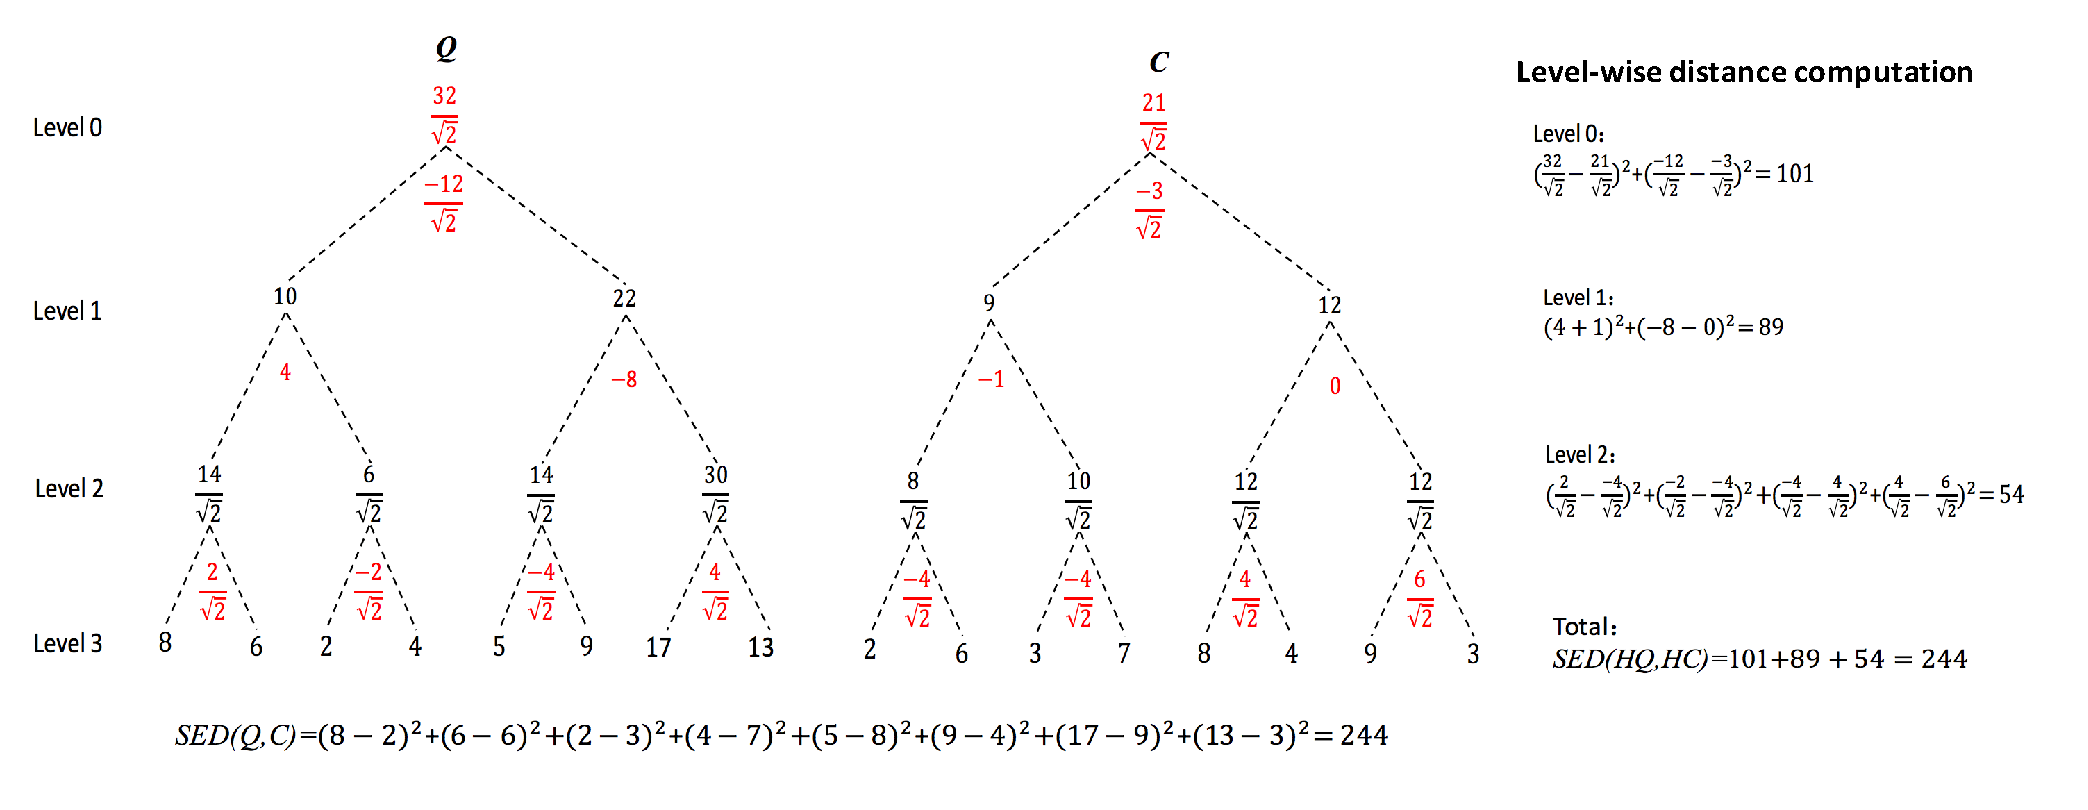
\includegraphics[width=0.95\textwidth]{Fig/chapter4/distance}
	\caption{基于Haar小波系数的距离计算示例}
	\label{fig-chapter4-distance}
\end{figure}

图\ref{fig-chapter4-distance}针对引理\ref{theory:dis}给出了示例说明。假定给定查询时间序列${\cal Q} = \{8, 6, 2, 4, 5, \\9, 17, 13\}$,
另一条序列为${\cal C}=\{2, 6, 3, 7, 8, 4, 9, 3\}$。通过计算可得,这两条序列间的欧式距离为$244$。接着,我们队这两条序列分别进行哈尔小波变换分别得到如图所示的两颗误差树。对每一层的系数进行欧式距离计算分别得到距离值101、89和54。其中第$0$层计算时把最终的均值也算进去了。通过计算发现系数的累加和确实等于原始序列的欧式距离。

\subsection{基于哈尔小波的欧式距离上、下界}
上一节介绍了,利用完整的哈尔小波系数,即全部的概要数据,能够用来计算原始的轨迹间欧式距离。但全部概要数据的数据量于原始轨迹数据量相同,不能达到降低通信开销的目的。为此
本节将介绍如何利用部分概要来计算轨迹的上、下界。首先根据引理\ref{theory:dis},我们有:
\begin{eqnarray}\label{eq:match}
SED({\cal Q},{\cal C}) &=& \sum\nolimits_{i=0}^{L-1}SED_{i}({\cal Q},{\cal C}) \nonumber\\ 
           &=&\sum\nolimits_{i=0}^{l}SED_{i}({\cal Q},{\cal C})+\sum\nolimits_{i=l+1}^{L-1}SED_{i}({\cal Q},{\cal C})
\end{eqnarray}

假设远程结点由粗到细已经获取了查询轨迹$\cal Q$的前$l+1$层概要数据,我们的目标就是根据这些已有的数据计算出$\cal Q$与任一候选$\cal C$的欧式距离上、下界。公式 \ref{eq:match}有半部分分为两部分,前半部分可以根据已有概要数据计算出来,后半部分无法直接计算。为此,我们将后半部分继续展开,得到如下:
\begin{eqnarray}\label{eq:decompose}
\sum_{i=l+1}^{L-1}SED_{i}({\cal Q},B)= \sum_{i=l+1}^{L-1}\sum_{j=0}^{2^i-1}(||\vd_{i,j}^{\cal Q}||^2+||\vd_{i,j}^{\cal C}||^2 -
2  \vd_{i,j}^{\cal Q} \bigcdot \vd_{i,j}^{\cal C}) 
\end{eqnarray}

公式\ref{eq:decompose}右半部分含有3个元素,第一个元素为查询轨迹$\cal Q$ 剩下概要数据的和, 该值可根据已有概要数据计算出来,计算方法为$SSQ-\sum_{i=0}^{l}\sum_{j=0}^{2^i-1}||\vd_{i,j}^{\cal Q}||^2$,其中$SSQ$为$\cal Q$所有系数的累加和。远程结点只需一开始就把$SSQ$发给所有远程结点即可。同理,第二个元素可在远程结点计算出来。难点在于对第三个关于系数內积累加和的计算。本文的做法是使用两次柯西—施瓦茨不等式估计其区间。第一次使用具体过程如下:
\begin{eqnarray}\label{eq:suofang1}
	-2\sum_{i=l+1}^{L-1}\sum_{j=0}^{2^i-1} ||\vd_{i,j}^{\cal Q}||\cdot ||\vd_{i,j}^{\cal C}||
	\le  \sum_{i=l+1}^{L-1}\sum_{j=0}^{2^i-1} -2\vd_{i,j}^{\cal Q}\bigcdot \vd_{i,j}^{\cal C} 
	\le  2\sum_{i=l+1}^{L-1}\sum_{j=0}^{2^i-1} ||\vd_{i,j}^{\cal Q}||\cdot ||\vd_{i,j}^{\cal C}||
\end{eqnarray}
接着我们对$\sum_{i=l+1}^{L-1}\sum_{j=0}^{2^i-1} ||\vd_{i,j}^{\cal Q}||\cdot ||\vd_{i,j}^{\cal C}||$进行再次使用柯西-施瓦茨不等式放缩:
\begin{eqnarray}\label{eq:suofang2}
\sum_{i=l+1}^{L-1}\sum_{j=0}^{2^i-1} ||\vd_{i,j}^{\cal Q}||\cdot ||\vd_{i,j}^{\cal C}|| \le 
	\sqrt{\sum_{i=l+1}^{L-1}\sum_{j=0}^{2^i-1}||\vd_{i,j}^{\cal Q}||^2} \cdot \sqrt{\sum_{i=l+1}^{L-1}\sum_{j=0}^{2^i-1}||\vd_{i,j}^{\cal C}||^2}
\end{eqnarray}
结合公式\ref{eq:suofang1}和\ref{eq:suofang2},我们得到如下完整的对$\sum_{i=l+1}^{L-1}\sum_{j=0}^{2^i-1} -2\vd_{i,j}^{\cal Q}\bigcdot \vd_{i,j}^{\cal C} $计算出如下上、下界。
 \begin{eqnarray}\label{eq:bound}
&&-2\sqrt{\sum_{i=l+1}^{L-1}\sum_{j=0}^{2^i-1}||\vd_{i,j}^{\cal Q}||^2} \cdot \sqrt{\sum_{i=l+1}^{L-1}\sum_{j=0}^{2^i-1}||\vd_{i,j}^{\cal C}||^2} \nonumber \\
&& 
\le  \sum_{i=l+1}^{L-1}\sum_{j=0}^{2^i-1} -2\vd_{i,j}^{\cal Q}\bigcdot \vd_{i,j}^{\cal C} 
\le  2\sqrt{\sum_{i=l+1}^{L-1}\sum_{j=0}^{2^i-1}||\vd_{i,j}^{\cal Q}||^2} \cdot \sqrt{\sum_{i=l+1}^{L-1}\sum_{j=0}^{2^i-1}||\vd_{i,j}^{\cal C}||^2}
\end{eqnarray}
最终,我们对欧式距离获得如下上、下界:
\allowdisplaybreaks
\begin{align} \label{eq:HaarBound}
&&	HLB_{l}({\cal Q},{\cal C}) =\sum_{i=0}^{l}SED_{i}({\cal Q},{\cal C})+
\sum_{i=l+1}^{L-1}\sum_{j=0}^{2^i-1}(||\vd_{i,j}^{\cal Q}||^2+||\vd_{i,j}^{\cal C}||^2)+ S_{0}({\cal Q},{\cal C}) \\
&&  - 2\sqrt{\sum_{i=l+1}^{L-1}\sum_{j=0}^{2^i-1}||\vd_{i,j}^{\cal Q}||^2} \cdot \sqrt{\sum_{i=l+1}^{L-1}\sum_{j=0}^{2^i-1}||\vd_{i,j}^{\cal C}||^2} \nonumber \\
&&	HUB_{l}({\cal Q},{\cal C}) = \sum_{i=0}^{l}SED_{i}({\cal Q},{\cal C})+
\sum_{i=l+1}^{L-1}\sum_{j=0}^{2^i-1}(||\vd_{i,j}^{\cal Q}||^2+||\vd_{i,j}^{\cal C}||^2)+S_{0}({\cal Q},{\cal C}) 
\nonumber \\
&&\qquad \quad + 2\sqrt{\sum_{i=l+1}^{L-1}\sum_{j=0}^{2^i-1}||\vd_{i,j}^{\cal Q}||^2} \cdot \sqrt{\sum_{i=l+1}^{L-1}\sum_{j=0}^{2^i-1}||\vd_{i,j}^{\cal C}||^2}
\end{align}
\allowdisplaybreaks[4]

进一步的我们提出两个性质,这两个性质表明我们的上、下界会随着概要数据的增加而越来越紧。它们的证明过程见本章附件。
\begin{theorem}[]\label{theory:lower}
	$HLB$会随着粒度的概要数据粒度的增加而逐渐上升,即$HLB_{l} \le HLB_{l+1}$。
	%The lower bound $HLB$  is non-decreasing when we move from level $l$ to ${l+1}$, i.e., $HLB_{l} \le HLB_{l+1}$.
\end{theorem}

\begin{theorem}[]\label{theory:upper}
	$HUB$会随着粒度的概要数据粒度的增加而逐渐下降,即$HUB_{l} \ge HUB_{l+1}$。
%	The upper bound $HUB$ is non-increasing when we move from level $l$ to  ${l+1}$, i.e., $HUB_{l} \ge HUB_{l+1}$.
\end{theorem}

\begin{figure}
	\centering
	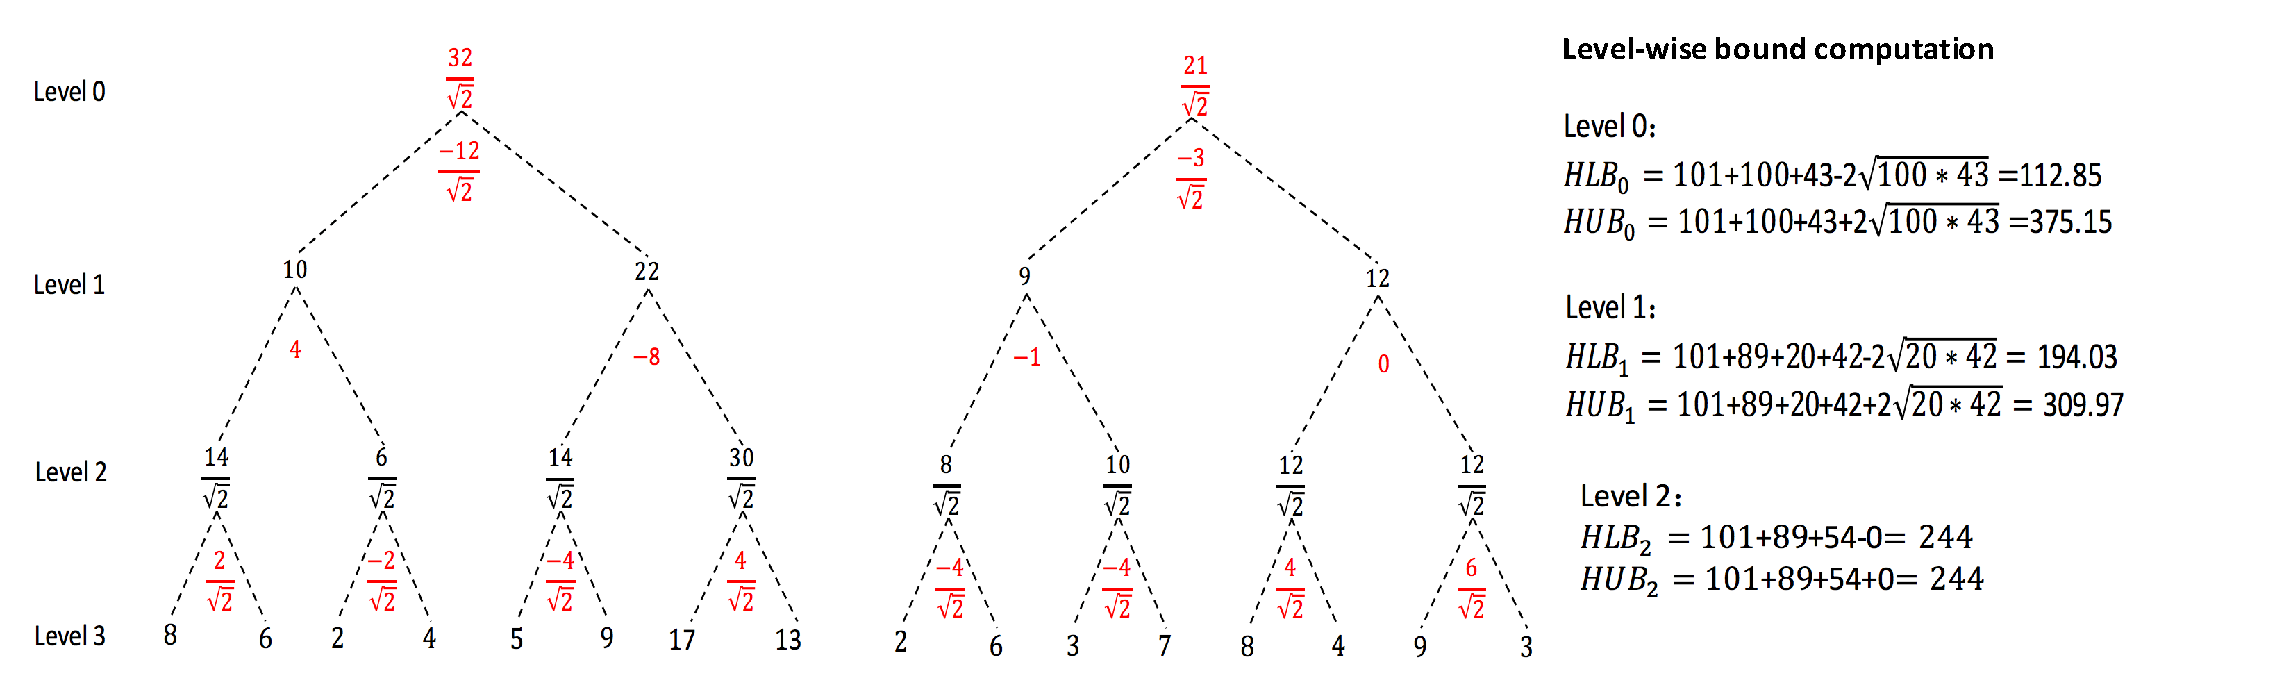
\includegraphics[width=0.95\textwidth]{Fig/chapter4/bound}
	\caption{欧式距离上、下界示例}
	\label{fig-chapter4-bound}
\end{figure}

图\ref{fig-chapter4-bound}介绍了使用概要数据得到越来越紧的上、下界,并直至逼近到真实距离的过程。其使用的数据与图\ref{fig-chapter4-distance}一样。当查询对象的第$0$层系数(数据量为1)发送给远程结点后,远程结点可以对其局部时间序列$\cal C$根据公式\ref{eq:HaarBound},计算得到上界和下界分别为$375.15$和$112.85$。当第$1$层系数(数据量为2)发过去后得到更紧的上界和下界分别为$309.97$和$194.03$。当第$2$层系数(即最后一层)发过去后,可以发现此时的上、下界等于真实的距离值。

 \section{基于欧式距离的查询算法:ED-FTB}\label{sec-c4-algorithm}
 \subsection{ED-FTB算法实现}
\begin{algorithm}[t]
	\renewcommand{\baselinestretch}{1}
	\caption{{\sl ED-FTB}\label{alg:EDCoordinator}在协调者结点}
	\begin{algorithmic}[2]
		\STATE /* \emph{ED-FTB协调者结点函数接口实现} */
	\end{algorithmic}
	\textbf{coordinatorInit}(${\cal Q} ,  {\cal R}$)
	\begin{algorithmic}[1]
		\STATE  $l\leftarrow -1$;
		\STATE $HQ \leftarrow$ Haar wavelet coefficients of $\cal Q$;\COMMENT{待查询轨迹获取哈尔小波系数}
		\STATE $SSQ = \sum_{i=0}^{n-1}||HQ_{i}||^2$;\COMMENT{所有系数的平方和}
		%		\STATE $l\leftarrow -1$;
		\STATE 	\textsf{sendToRemoteSites}(${\cal R}$, $SSQ$);
	\end{algorithmic}
	
	\textbf{generateInfo()}
	\begin{algorithmic}[1]
		\STATE $l\leftarrow l+1$;
		\STATE return $\widehat {\cal Q}_{l}$;\COMMENT{返回第$l$层哈尔小波系数}
	\end{algorithmic}
\end{algorithm}

\begin{algorithm}[t]
	\renewcommand{\baselinestretch}{1}
	\caption{{\sl ED-FTB}\label{alg:EDRemote}在远程结点}
	\begin{algorithmic}[2]
		\STATE /* \emph{ED-FTB远程结点函数接口实现} */
	\end{algorithmic}
	
	\textbf{remoteInit($TS_{r} , S_{r}$)}
	\begin{algorithmic}[1]
		\IF{第一次接受查询}
		\FORALL{ $\cal C$ in $TS_{r}$}
		\STATE $HC \leftarrow$ Haar wavelet coefficients of $\cal C$; \COMMENT{候选轨迹获取哈尔小波系数}
		\STATE $SSC = \sum_{i=0}^{n-1}||HQ_{i}||^2$;\COMMENT{所有系数的平方和}	   
		\ENDFOR
		\ENDIF
		\FORALL{ $\cal C$ in $TS_{r}$}
		\STATE $C\_BF \leftarrow  \langle 0,\infty \rangle$; \COMMENT {为$\cal C$初始化界特征}
		\STATE $S_{r}=S_{r} \cup C\_BF$;
		\ENDFOR
		\STATE $SSQ \leftarrow$\textsf{getFromCoordinator}();
	\end{algorithmic}
	
	\textbf{updateBounds}($S_{r}$, $M$) //边更新界边剪枝。
	\begin{algorithmic}[1]
		\FORALL{ $\cal C$ in $TS_{r}$}
		\STATE  $a=\sum_{i=l+1}^{L-1}\sum_{j=0}^{2^i-1}||\vd_{i,j}^{\cal Q}||^2$;$b=\sum_{i=l+1}^{L-1}\sum_{j=0}^{2^i-1}||\vd_{i,j}^{\cal C}||^2$;
		\STATE $tmp=a+b+S_{0}(\cal Q, \cal C)$;
		\STATE $lb=tmp -2\sqrt{ab}$;$ub=tmp+2\sqrt{ab}$;
		\IF{$ lb<gkub \quad \&\& \quad  (lb=lb+ \sum_{0}^{l}SED_{i}({\cal Q},{\cal C}))<gkub$}
		\STATE 将轨迹$\cal C$的界特征的下界更新为$lb$;
		\IF{$ub<gkub \quad \&\& \quad (ub=ub+ \sum_{0}^{l}SED_{i}({\cal Q}, {\cal C}))<gkub)$}
		\STATE $ ub=ub+ \sum_{0}^{l}SED_{i}({\cal Q}, {\cal C})$;
		\STATE 将轨迹$\cal C$的界特征的上界更新为$ub$;
		\ENDIF
		\ELSE
		\STATE 将该轨迹从$S_{r}$中移除;
		\ENDIF
		\ENDFOR
	\end{algorithmic}
\end{algorithm}

在上一节,我们已经利用概要数据提出了欧氏距离的上、下界。这使得在FTB框架中插入欧式距离成为可能。本节将详细介绍将欧式距离跟FTB相结合的查询算法ED-FTB。ED-FTB维持了FTB框架的主要结构,只对本章第一节所介绍的接口进行了具体实现。

算法\ref{alg:EDCoordinator}介绍了协调者节点的上的函数接口的实现方法。在\textsf{coordinatorInit}函数中,我们对待查询轨迹进行哈尔小波变换,并计算出其所有系数的平方和。接着将该平方和发送给所有远程结点。远程结点在将来将会利用该值进行上、下界计算。
由于FTB框架是迭代式由粗到细的通信计算框架,在每轮的迭代中会将某一层的概要数据(哈尔小波系数)发送给远程结点。因此,在初始化过程中我们用$l$来记录当前已经发送到哪一层的数据,并将$l$初始化为$-1$以便从第0层开始。此外,我们在\textsf{generateInfo}中准备将要发送的下一层概要数据,以便协调者结点发送。

接着,算法\ref{alg:EDRemote}介绍运行在远程结点的函数。对于\textsf{RemoteInit}函数,若远程结点是第一次接受查询,则会为每条候选轨迹进行哈尔小波变换并计算系数的平方和。若不是,则为该结点所包含的每条轨迹初始化界特征信息(下界初始化为0,上界初始化为正无穷),并接受查询轨迹的系数平方和。在查询执行过程中\textsf{UpdateBounds}函数为候选更新上、下界。直接实现方式为根据上、下界的计算公式,计算出这两个值。但由于查询过程中的主要计算开销就是对所有候选更新界特征。所以,降低该过程的计算开销很有必要。

为降低更新界特征的计算开销,本文引入了在更新界过程中进行剪枝的思想。在介绍此方法前,我们再次回顾下我们的下界。我们的下界计算主要包含3个算子:首先是$\sum_{i=0}^{l}SED_{i}({\cal Q},{\cal C})$,其计算复杂度为O($2^{l}$)。其次是$\sum_{i=l+1}^{L-1}\sum_{j=0}^{2^i-1}||\vd_{i,j}^{\cal Q}||^2$,由于该部分可以通过$SSQ-\sum_{i=0}^{l}\sum_{j=0}^{2^i-1}||\vd_{i,j}^{\cal Q}||^2$计算,而且$\sum_{i=0}^{l-1}\sum_{j=0}^{2^i-1}||\vd_{i,j}^{\cal Q}||^2$的值已知。故该部分的计算复杂度也为$O(2^{l})$。同理,第三部分$\sum_{i=l+1}^{L-1}\sum_{j=0}^{2^i-1}||\vd_{i,j}^{\cal C}||^2$计算复杂度也为$O(2^{l})$。除这三个算子的计算法外,剩余部分的计算复杂度为$O(1)$。

基于以上分析。假设我们已知若轨迹下界值超过$\alpha$,那该条轨迹即不可能称为候选。此时,我们可以在更新下界的同时进行剪枝(算法\ref{alg:EDRemote}:\textsf{UpdateBounds}函数)。具体的做法是我们首先计算出第二和第三两个算子,并根据这两个算子的值计算出下界中除$\sum_{i=0}^{l}SED_{i}({\cal Q},{\cal C})$以外部分的值。若此时计算出来的值已超过$gkub$,则无需继续求解下界和上界,直接将该候选删除。若仍小于$gkub$,则计算出完整的下界,并判断此时下界值是否小于$gkub$,若小于则停止计算上界并将该候选删除。当更新完下界后,我们先计算出上界中除$\sum_{i=0}^{l}SED_{i}({\cal Q},{\cal C})$以外部分的值。若该部分值超过$gkub$,则该轨迹的上界对选取新一轮的全局最小的$k$个上界没有帮助,无需计算该轨迹的具体上界值。否则,计算出具体的上界并更新界特征。此时,需要注意的是,在FTB框架算法的第7-9行中,我们仅需传递上界小于 $gkub$的$k$个最小上界。若个数不足$k$个,则只传递满足$gkub$的上界。
 
 \subsection{ED-FTB算法性能分析}
 在分析前,我们先介绍对比算法LEEWAVE-CL。LEEWAVE-CL是在LEEWAVE算法的基础上使用了本文所提下界(比原始的下界更紧)。LEEWAVE-CL算法也是迭代式算法。在它的每次迭代中,远程结点根据获取的概要数据,为每个候选计算如下两个算子:$\sqrt{\sum_{i=l+1}^{L-1}\sum_{j=0}^{2^i-1}||\vd_{i,j}^{\cal C}||^2}$ 和  $S_{0}({\cal Q},{\cal C})+\sum_{i=0}^{l}SED_{i}({\cal Q},{\cal C})$。然后协调者节点获取者些参数并为每个候选计算上、下界,并利用界特征进行过滤。然后,将候选列表发给对应远程结点。LEEWAVE-CL方法与本文方法的最大不同就是,它在协这结点进行界特征的计算和过滤,而ED-FTB是在所有远程结点进行。接下来,我们将从时间和通信两个方面对ED-FTB和LEEWAVE-CL进行对比分析。在此之前,我们使用如下标记:(i)使用$|C_{i}|$ 和 $|CS_{i}|$ 分别表示第$i$($i\ge 0$)次迭代前候选轨迹的数量和包含候选轨迹的远程结点数量。由于采用相同的上、下界,这两个算法的迭代次数相同,我们假定迭代次数为$\lambda$($\lambda \le \log_{2}n$)。
 
  \textbf{时间复杂度:}不考虑系统初始化时对所有候选进行哈尔小波变换的时间开销, ED-FTB和LEEWAVE-CL两者的时间开销来自迭代式计算时更新上、下界,所以他们的时间复杂度一样。计算复杂度最坏的情况就是所有候选都集中在一个结点上,则更新上、下界的时间复杂度为$O(\sum_{i=0}^{\lambda-1} d\cdot |C_{i}| \cdot 2^{i})$。此外,由于$k$值一般较小,算法运行过程中涉及到的查找局部最小的$k$个上界耗时较低,可以忽略。总的来说,ED-FTB和LEEWAVE-CL的时间复杂度均为$O(\sum_{i=0}^{\lambda-1} d\cdot |C_{i}| \cdot 2^{i})$。但ED-FTB由于在各个结点进行界特征的计算,且采用了边计算边过滤的策略,故其实际计算开销低于LEEWAVE-CL。
 
  \textbf{通信复杂度:}
ED-FTB和LEEWAVE-CL的通信开销主要集中在迭代式计算过程中。ED-FTB在第$i$轮迭代时,需要花费$O(d\cdot 2^{i}\cdot |CS_{i}|+|C_{i}|)$ 代价以将第$i$层概要数据发送给候选结点,并至多接收$|C_{i}|$个上界(用于计算全局的剪枝阈值)。在$\lambda$次迭代后,总的通信开销为$O(\sum_{i=0}^{\lambda-1}(d \cdot 2^{i} \cdot|CS_{i}| + |C_{i}|))$。
LEEWAVE-CL 在第$i$轮迭代需要花费 $O(|CS_{i}| \cdot (d\cdot 2^{i}+ |C_{i+1}|))$ 来讲概要数据和所有候选的列表发送给所有候选结点。此外,还需要花费$O(d\cdot |C_{i+1}|)$代价以接受每个候选轨迹的两个算子值以便在协调者结点计算出上、下界。所以,当$\lambda$次迭代后,其总的通信开销为$O(|CS_{i}| \cdot (d\cdot 2^{i}+ |C_{i+1}|)+d\cdot |C_{i+1}|)$。对比两个算法的开销值,我们可以发现ED-FTB的能节省更多通信开销。
 
 \section{实验分析}\label{sec-c4-Exp}
本节将在真实世界的轨迹数据上评估本章节所提出的算法。本小节首先介绍使用的真实世界轨迹数据集及实验设置。接着从分别验证了算法的有效性和可扩展性。

\subsection{实验设置}
本章工作在实验中使用北京出租车数据集,该数据集已被广泛应用于轨迹数据分析。该数据集采集了北京市三万多辆出租车在2013年10月份到12月份三个月内的行驶GPS轨迹。每个GPS轨迹点包含的数据维度较多,我们仅选取了位置(经度和纬度)、时间、速度和角度这五个维度的值,并进行了归一化预处理。我们从该数据集中截取了两个子数据集:\emph{T-Small}和\emph{T-Big}以分别验证算法的有效性和可扩展性。
\emph{T-Small}截取了10月1至7号间 上午8点到10点的轨迹数据,并从中选出最长的1万条轨迹进行分析。
\emph{T-Big} 截取了11月1号至12月31号间每天上午8至10点和下午5至7点两个时间段的1百万条轨迹数据。为满足实验需求,这两个数据集的每条轨迹长度均超过4,096。

在本章的实验中,我们将比较ED-FTB和LEEWAVE-CL算法的性能。LEEWAVE-CL算法在已有LEEWAVE算法的基础上使用了本文所提供的下界。
两个算法均用JAVA实现,并运行在一个包含12个结点的Spark集群上。每个结点包含8核因特尔E5335 2.0 GHz中央处理器和16GB的内存。我们在\emph{T-Small}数据集上验证了算法的有效性,在\emph{T-Big} 数据集上验证了算法的可扩展性。
%All codes, written in Java, were evaluated on a 12-node clustering running Spark 1.5.2 over Ubuntu 12.0.4. Each node is equipped with an 8 cores Intel E5335 2.0GHz processor and 16GB memory.
%contains 1,000,000 trajectories from November 1st to December 31st during 8:00 to 10:00 am and 17:00-19:00 pm.
%每个轨迹点包含的数据维度较多,我们仅选取了位置(经度和纬度)、时间、速度和角度这五个维度的值,并进行了归一化预处理。


\subsection{算法有效性}

\begin{figure}[t]
	\centering
		\centering
		\subfigure[$k=1$]{
			\label{fig:EDpruk1}
			\includegraphics[width=2.7in]{Fig/chapter4/EDpruk1.eps}
		}
		\subfigure[$k=10$]{
			\label{fig:EDpruk10}
			\includegraphics[width=2.7in]{Fig/chapter4/EDpruk10.eps}
		}
	\\
		\subfigure[$k=50$]{
		\label{fig:EDpruk50}
		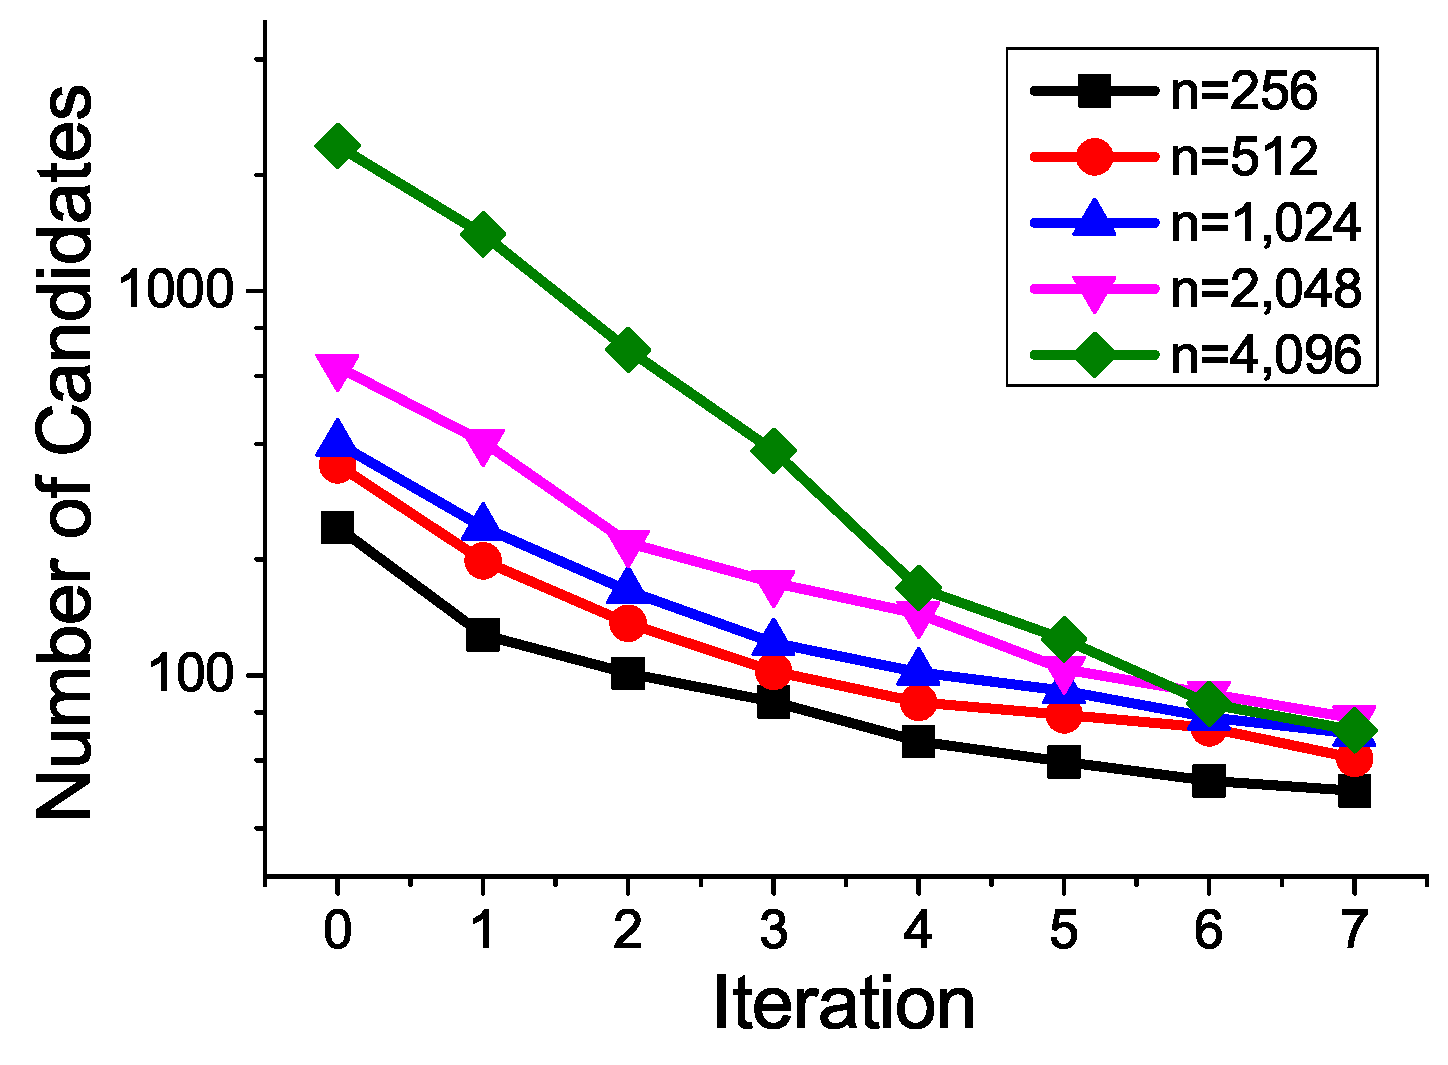
\includegraphics[width=2.7in]{Fig/chapter4/EDpruk50.eps}
		}
		\subfigure[$k=100$]{
			\label{fig:EDpruk100}
			\includegraphics[width=2.7in]{Fig/chapter4/EDpruk100.eps}
		}
		\caption{ED-FTB剪枝效果图}
		\label{fig:ED-DTKTS}
\end{figure}
首先,我们通过观察迭代过程中每轮结束后的剩余候选数来研究ED-FTB算法的剪枝效果。在该组实验中,我们将$M$设置为10,000,并研究了不同长度轨迹剪枝的效果。图 \ref{fig:ED-DTKTS} 介绍了前8轮迭代中每轮迭代后的候选数。我们可以看出候选数在前5轮迭代中下降的较快且已经过滤掉绝大多数候选。这说明了我们的上、下界收敛速度较快,具有较好的剪枝效果。此外,我们可以发现短轨迹在前几轮中候选数下降的比长轨迹快。这是由于相同数据量的概要数据下短轨迹比长轨迹包含更多的原始轨迹的信息。最后,对比不同的 $k$值,我们发现$k$值越小,每轮所剩候选数越少。即$k$越小,剪枝效果越好。这是由于$k$值越小,我们所获得的全局第$k$小上界值就越小。而无论$k$值如何选取,每个候选的下界值不变。因此,越小的全局上界能通过下界剪枝掉更多的候选。同时,由于实际应用中$k$值通常都是一个很小的数。因而我们的算法能往往取得较好的效果。
\begin{figure}
		\centering
	\subfigure[$k=1$]{
		\label{fig:EDprucmpk1}
		\includegraphics[width=2.7in]{Fig/chapter4/cmp1.eps}
	}
	\subfigure[$k=10$]{
		\label{fig:EDprucmpk10}
		\includegraphics[width=2.7in]{Fig/chapter4/cmp10.eps}
	}
\\
	\subfigure[$k=50$]{
		\label{fig:EDprucmpk50}
		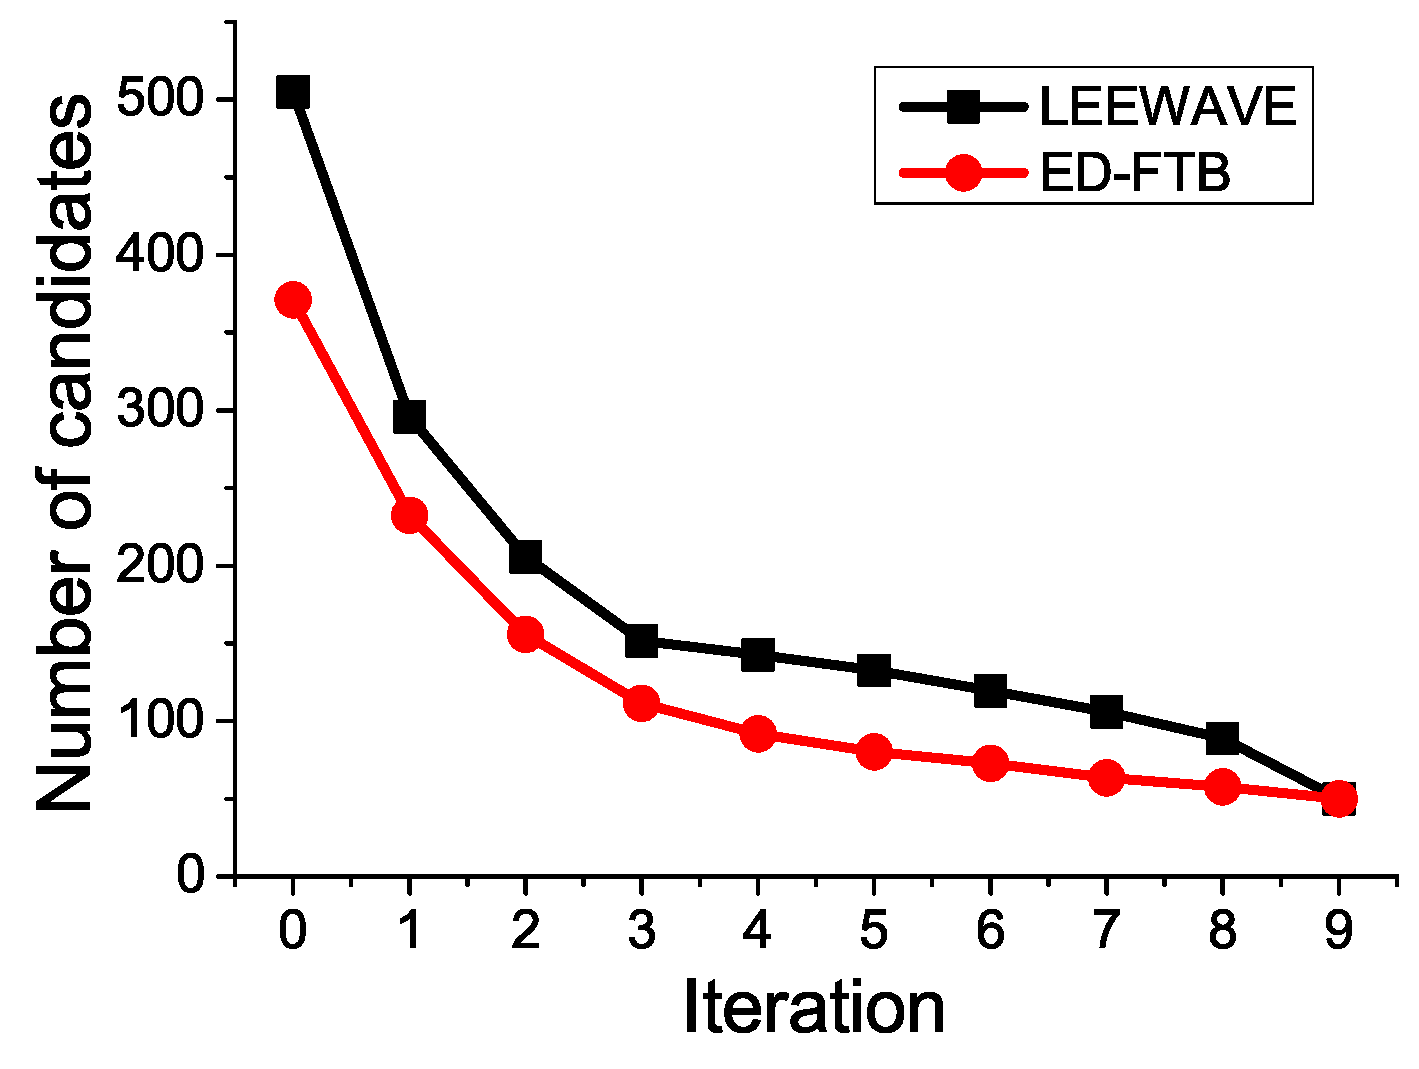
\includegraphics[width=2.7in]{Fig/chapter4/cmp50.eps}
	}
	\subfigure[$k=100$]{
		\label{fig:EDprucmpk100}
		\includegraphics[width=2.7in]{Fig/chapter4/cmp100.eps}
	}
	\caption{下界对剪枝结果的影响}
	\label{fig:PruningCmp}
\end{figure}

然后,我们对比研究了ED-FTB的剪枝效果和ED-FTB使用LEEWAVE中的下界后的剪枝效果,以分析下界对剪枝效果的影响。
在该组实验中,我们将$M$值设置为10,000,轨迹长度设为$1,024$。图\ref{fig:PruningCmp}对比展示了不同$k$值下,不同下界对剪枝的影响。其中LEEWAVE代表ED-FTB算法使用LEEWAVE算法中的下界后的结果。从图中,我们可以看出由于本文所提出的下界比已有算法的下界更紧,导致每轮迭代结束后ED-FTB所剩的候选数更少。这说明了本文所提下界的优越性。此外我们可以发现$k$值越小,两条曲线间的间隔越大。更能说明本文下界所取得的优越性越明显。


\begin{figure} [t]
	\centering
	\subfigure[$M=50,k=1$]{
		\label{50-1}
		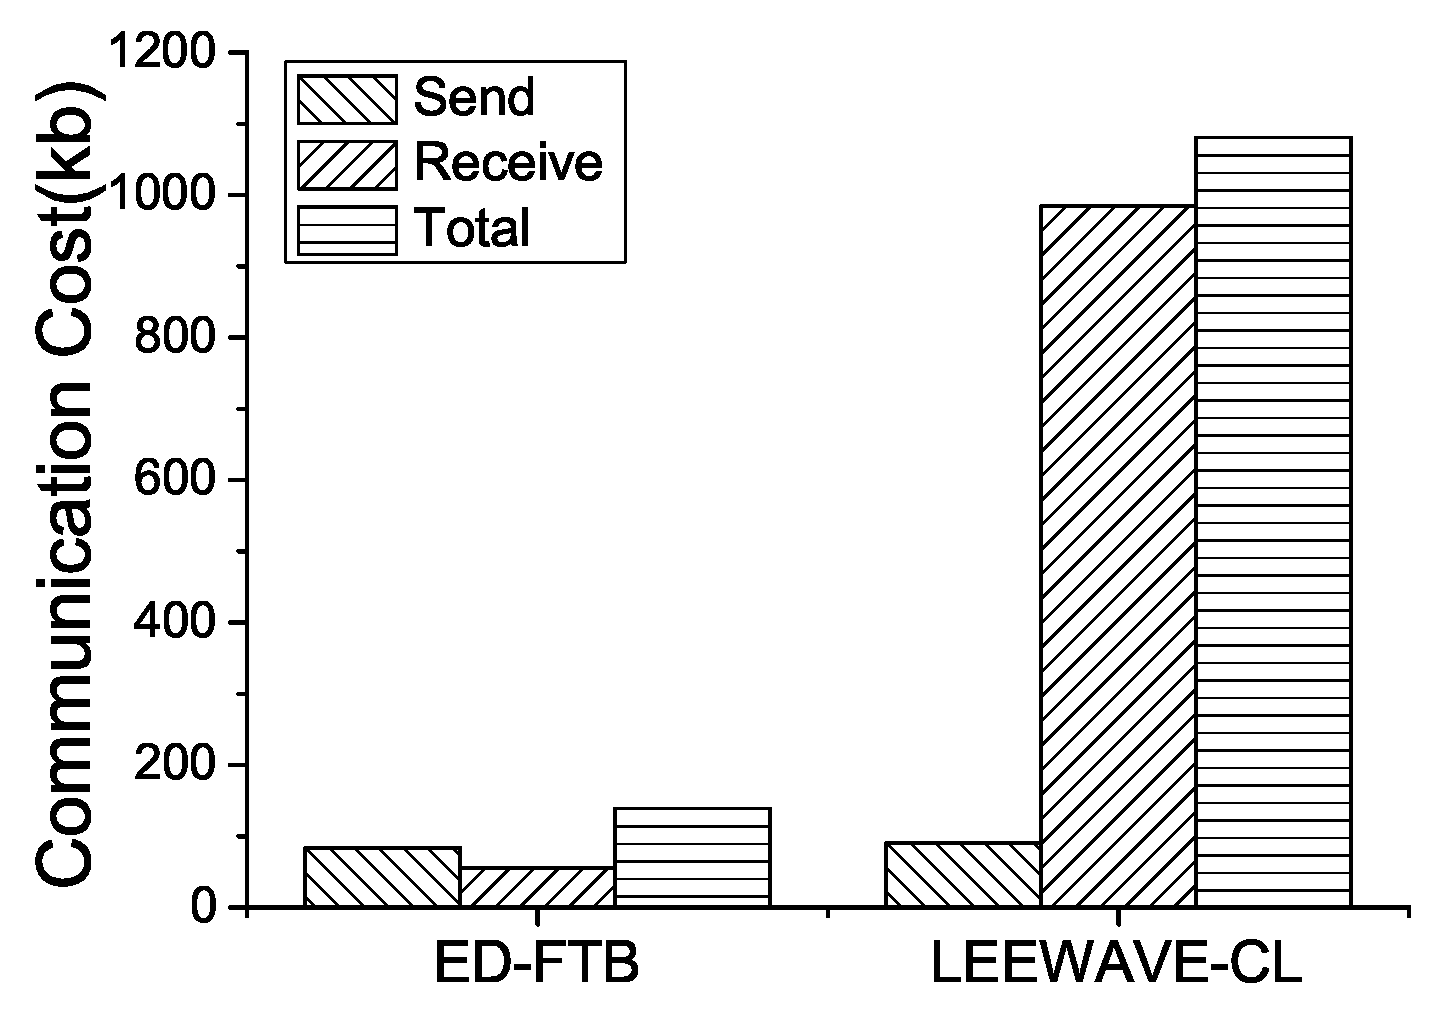
\includegraphics[width=2.7in]{Fig/chapter4/1k50m.eps}
	}
	\subfigure[$M=50,k=1,000$]{
		\label{50-1000}
		\includegraphics[width=2.7in]{Fig/chapter4/1000k50m.eps}
	}
	
	\subfigure[$M=200,k=1$]{
		\label{200-1}
		\includegraphics[width=2.7in]{Fig/chapter4/1k200m.eps}
	}
	\subfigure[$M=200,k=1,000$]{
		\label{200-1000}
		\includegraphics[width=2.7in]{Fig/chapter4/1000k200m.eps}
	}
	\vspace{-10pt}
	\caption{算法执行策略详细比较}
	\label{fig:components}
	\vspace{-0.5cm}
\end{figure}
接着,我们使用相同的界,对比了分析了本文所提查询策略与LEEWAVE所用查询策略对通信性能的影响。我们从协调者节点出发,研究了两种策略下它发送和接受的数据量以及总的数据通信开销。
图 \ref{fig:components}介绍了当$M$取50和$100$,k取$1$和$1000$下的实验结果。图中LEEWAVE-CL代表
结合了LEEWAVE的查询策略与本文的界特征后的算法。
从图中我们可以发现,协调者结点在两种策略下,发送的数据量差别不大且都比较小。这是因为,两个策略都有减少协调者数据发送的数据量这一共同目标。且两者使用的使用概要数据剪枝的策略很好的达成了这一目标。
但接受的数据量在两种策略下差别很大。ED-FTB所用的查询策略是在每个远程结点剪枝数据。每轮迭代完后远程结点仅需将所计算出来的局部最小的$k$个上界返回。而LEEAVE-CL需要将所有候选的跟计算界信息的两个算子返回。当远程结点所包含的数据越多,则两者的区别越大。特别地,当$k$值较小时(图 \ref{50-1} 和 \ref{200-1}),ED-FTB所收到的数据不到LEEWAVE-CL的十分之一。
%Especially, when $k$ is small(in Fig. \ref{50-1} and \ref{200-1}), the amount of data received in DT-KST is $10\%$ less than that of LEEWAVE-CL. 


\begin{figure}[t]
	\centering
		\centering
		\subfigure[$M=100$]{
			\label{fig:costM100}
			\includegraphics[width=2.7in]{Fig/chapter4/costM100.eps}
		}
		\subfigure[$M=1,000$]{
			\label{fig:costM1000}
			\includegraphics[width=2.7in]{Fig/chapter4/costM1000.eps}
		}
	\\
		\subfigure[$M=5,000$]{
		\label{fig:costM5000}
		\includegraphics[width=2.7in]{Fig/chapter4/costM5000.eps}
	}
		\subfigure[$M=10,000$]{
			\label{fig:costM10000}
			\includegraphics[width=2.7in]{Fig/chapter4/costM10000.eps}
		}
		\caption{$n$,$k$和$M$对ED-FTB算法通信开销的影响}
		\label{fig:costKM}
\end{figure}
其次,我们研究了$n$,$k$和$M$对ED-FTB算法通信开销的影响。在该组实验中,我们将$n$的值从256变化到$4,096$,将$k$的值从1变化到100。图\ref{fig:costKM}展示了不同$M$值下($M$从100编化到$10,000$),ED-FTB算法通信开销随参数变化的结果。首先,我们看出随着$k$值的增加,通信开销逐步增加。这是由于$k$值越大,每轮所剩候选数越多,候选所在的远程结点也就越多。从而每轮需要将概要数据发送到更多的候选结点中。其次,随着$n$值的增加通信开销也在增加。这是由于长轨迹需要发送更多的数据才能达到与短轨迹相同的剪枝效果。最后,对比三幅图可以发现,随着远程结点数据的增加,通信开销也在增加。这是由于在每轮迭代中,远程结点增加后,候选轨迹会分布到更多的结点中。因而,算法需要将概要数据发送到更多的结点中。因而总的通信开销也会增加。但是,对于极端情况$M=10,000$时,此时每个远程结点仅包含一条轨迹时我们的通信开销仍不到$10$Mb,远小于直接方法的开销(约$640$Mb)。因此,ED-FTB算法具有较高的通信节约性能。

\begin{figure}[t]
\centering
\subfigure[$k=1$]{
	\label{fig:costCmpk1}
	\includegraphics[width=2.7in]{Fig/chapter4/cmpk1.eps}
}
\subfigure[$k=10$]{
	\label{fig:costCmpk10}
	\includegraphics[width=2.7in]{Fig/chapter4/cmpk10.eps}
}
\\
\subfigure[$k=50$]{
	\label{fig:costCmpk50}
	\includegraphics[width=2.7in]{Fig/chapter4/cmpk50.eps}
}
\subfigure[$k=100$]{
	\label{fig:costCmpk100}
	\includegraphics[width=2.7in]{Fig/chapter4/cmpk100.eps}
}
\caption{算法性能比较}
\label{fig:costCmp}
\end{figure}
接下来,我们将ED-FTB与LEEWAVE和LEEWAVE-CL进行通信性能比较。在该组实验中我们将轨迹长度$n$从256变化到$4,096$。图\ref{fig:costCmp}展示了当$k$取值为1,10和100下的结果。从该组图中我们可以看出,本文所提ED-FTB算法性能最好,LEEWAVE-CL其次,最差的是LEEWAVE。LEEWAVE-CL比LEEWAVE好的原因是它使用了本文所提下界进行剪枝。本文所提下界由于比LEEWAVE中的更加紧凑,因而剪枝效果更好。最终导致通信开销更低。而ED-FTB算法比LEEWAVE-CL好的原因是,本文采用的是在远程结点剪枝的策略,只需发送概要数据。而LEEWAVE和LEEWAVE-CL 均是采用在协调者结点剪枝的策略,除了发概要数据还要发送和接受其他额外数据。因而开销更高。最后,我们可以发现,随着轨迹长度$n$和$k$值的增加,EDD-FTB算法所节省的通信开销逐步增大。这进一步说明了本文算法的优越性。

\subsection{算法可扩展性}
\begin{figure} [t]
	\centering
	\subfigure[Running time in respect of $n$,$N$]{
		\label{fig:KLN}
		\includegraphics[width=2.7in]{Fig/chapter4/edtimeScalability.eps}		
	}
	\subfigure[Communication cost in respect of  $n$,$N$]{
		\label{fig:MN}
		\includegraphics[width=2.7in]{Fig/chapter4/edcommScalability.eps}
	}
	\caption{ED-FTB 算法可扩展性 {(T-Big数据集)}}
	\label{fig:EDScalability}
\end{figure}

 本小节我们将在\emph{T-Big}数据集上从时间和通信两个角度研究了ED-FTB算法的可扩展性。首先,考虑了轨迹数量$N$(即数据量大小)和轨迹长度$n$对可扩展性的影响。
在该组实验中,我们将$k$设置为1,$M$设置为$10,000$。我们将轨迹长度从$256$到$4096$进行指数级变化,同时将轨迹数量从10万到1百万进行线性增加。
  图\ref{fig:EDScalability}分别对这两个角度的结果进行了介绍,其中图\ref{fig:KLN}介绍了时间性能受$n$和$N$的影响(时间包系统初始化过程中对数据进行哈尔小波转换的开销)。我们可以看到对于任意长度的轨迹数据集,ED-FTB算法的运行时间都随着轨迹数据量的增加而线性增加。
  此外,随着轨迹长度的指数增加,算法的运行时间也指数增加,即运行时间与轨迹长度呈一定的线性关系。这一结果反映了由于ED-FTB的剪枝效果较好,导致迭代结束后,所剩候选数较少。即我们对ED-FTB算法时间复杂度分析部分的$N'$较少。结合以上两点,我们可以看出ED-FTB算法运行时间随着数据集的大小而线性变换,因此运行效率具有较好的可扩展性。

\section{本章小结}\label{sec-c4-conclusion}
本章节介绍了利用FTB框架在嵌入欧式距离下的具体实现算法ED-FTB。本章节,首先针对欧式距离,提出了基于哈尔小波系数的概要数据。接着,提出了基于哈尔小波系数的欧式距离上、下界。
该上、下界能够随着小波粒度的增加而逐渐变紧,这使得我们利用将该距离嵌入到FTB框架称为可能。为此,我们提出了ED-FTB算法以实现基于欧式距离的查询。在我们的查询算法中,我们引入了边计算下界边剪枝的查询优化措施,以提高执行效率。通过在真实数据集上进行的实验,表明所提方法剪枝效果由于现有方案,且具有较好的可扩展性。

\section*{本章证明附件}\label{sec-c4-Appendix}
\textbf{引理 \ref{theory:dis}. }{\em 给定两条轨迹${\cal Q}$ 和 ${\cal C}$,$H{\cal Q}$ 和 $H{\cal C}$分别表示${\cal Q}$ 和 ${\cal C}$经过哈尔小波变换后的系数序列。我们有如下结论:$SED({\cal Q},{\cal C})=SED(H{\cal Q},H{\cal C})$。}
\begin{proof}
	首先,根据$S_{i}({\cal Q}, {\cal C})$ 和 $SED_{i}({\cal Q}, {\cal C})$定义(定义\ref{eq:basic})我们有
	\allowdisplaybreaks
	\begin{eqnarray}
	&&	S_{i+1}({\cal Q}, {\cal C})=\sum\nolimits_{j=0}^{2^{i+1}-1}SED(\va_{i+1,j}^{\cal Q},\va_{i+1,j}^{\cal C}) \nonumber \\
	&=&SED(\va_{i+1,0}^{\cal Q},\va_{i+1,0}^{\cal C}) + SED(\va_{i+1,1}^{\cal Q},\va_{i+1,1}^{\cal C}) + \cdots + \nonumber \\
	&\,& SED(\va_{i+1,2^{i+1}-2}^{\cal Q},\va_{i+1,2^{i+1}-2}^{\cal C}) + 	SED(\va_{i+1,2^{i+1}-1}^{\cal Q},\va_{i+1,2^{i+1}-1}^{\cal C}) \nonumber \\
	&=&SED(\va_{i,0}^{\cal Q},\va_{i,0}^{\cal C})  +   SED(\vd_{i,0}^{\cal Q}, \vd_{i,0}^{\cal C})   + \cdots+\nonumber \\
	&\,& SED(\va_{i,2^{i}-1}^{\cal Q},\va_{i,2^{i}-1}^{\cal C})  +   SED(\vd_{i,2^{i}-1}^{\cal Q}, \vd_{i,2^{i}-1}^{\cal C})  \nonumber   \nonumber \\
	&=& \sum\nolimits_{j=0}^{2^i-1}SED(\va_{i,j}^{\cal Q}, \va_{i,j}^{\cal C})+ \sum\nolimits_{j=0}^{2^i-1}SED(\vd_{i,j}^{\cal Q}, \vd_{i,j}^{\cal C})\nonumber \\
	&=&S_{i}({\cal Q}, {\cal C})+SED_{i}({\cal Q},{\cal C})
	\end{eqnarray}
	\allowdisplaybreaks[4]
根据如上公式,对于叶子层结点,我们有:
	\begin{eqnarray} \label{eq:prove1L}
	S_{L}({\cal Q},{\cal C})&=&S_{0}({\cal Q},{\cal C})+ \sum\nolimits_{i=0}^{L-1}{SED_{i}({\cal Q},{\cal C})} \nonumber \\
	&=& SED(H{\cal Q},H{\cal C})
	\end{eqnarray}
	此外,第$L$层为叶子节点层,包含了轨迹的原始信息。所以我们又有$SED({\cal Q},{\cal C}) = S_{L}({\cal Q},{\cal C})$。此时结合公式\ref{eq:prove1L}
	我们得到 $SED({\cal Q},{\cal C})=SED(H{\cal Q},H{\cal C})$。原问题得证。
\end{proof}

\textbf{定理 \ref{theory:lower}. }{\em $HLB$会随着粒度的概要数据粒度的增加而逐渐上升,即$HLB_{l} \le HLB_{l+1}$。}
至此,我们根据哈尔小波变换得到原始轨迹不同粒度概要数据,并根据概要数据提出了欧式距离的上、下界。


\begin{proof}\label{proof:p2}
	我们的策略是证明 $HLB_{l+1}- HLB_{l}\ge 0$。我们首先将其左半部分展开:
	\begin{eqnarray}\label{eq:minus}
HLB_{l+1}- HLB_{l}= SED_{l+1}({\cal Q},{\cal C}) - \sum\nolimits_{j=0}^{2^{l+1}-1}(||\vd_{l+1,j}^{\cal Q}||^2  + ||\vd_{l+1,j}^{\cal C}||^2)+\nonumber\\
 2(\sqrt{\sum_{i=l+1}^{L -1}\sum_{j=0}^{2^i-1}||\vd_{i,j}^{\cal Q}||^2} \cdot \sqrt{\sum_{i=l+1}^{L -1}\sum_{j=0}^{2^i-1}||\vd_{i,j}^{\cal C}||^2} -\sqrt{\sum_{i=l+2}^{L -1}\sum_{j=0}^{2^i-1}||\vd_{i,j}^{\cal Q}||^2} \cdot \sqrt{\sum_{i=l+2}^{L -1}\sum_{j=0}^{2^i-1}||\vd_{i,j}^{\cal C}||^2})\nonumber
	\end{eqnarray}	
	接着, 我们将$SED_{l+1}({\cal Q},{\cal C})$ 展开得到$SED_{l+1}({\cal Q},{\cal C})=\sum_{j=0}^{2^{l+1}-1}{(||\vd_{l+1,j}^{\cal Q}||^2+||\vd_{l+1,j}^{\cal C}||^2}-2 \vd_{l+1,j}^{\cal Q} \bigcdot \vd_{l+1,j}^{\cal C})$。我们的问题变为证明如下不等式成立。
	\begin{eqnarray}\label{eq:InEq}
	\sum_{j=0}^{2^{l+1}-1}\vd_{l+1,j}^{\cal Q} \bigcdot \vd_{l+1,j}^{\cal C} &\le& \sqrt{\sum_{i=l+1}^{L-1}\sum_{j=0}^{2^i-1}||\vd_{i,j}^{\cal Q}||^2} \cdot \sqrt{\sum_{i=l+1}^{L-1}\sum_{j=0}^{2^i-1}||\vd_{i,j}^{\cal C}||^2} \nonumber\\
&\quad&	-	\sqrt{\sum_{i=l+2}^{L-1}\sum_{j=0}^{2^i-1}||\vd_{i,j}^{\cal Q}||^2} \cdot \sqrt{\sum_{i=l+2}^{L-1}\sum_{j=0}^{2^i-1}||\vd_{i,j}^{\cal C}||^2} 
	\end{eqnarray}	
	对于不等式 \ref{eq:InEq}的左半部分我们有
	$\sum_{j=0}^{2^{l+1}-1}\vd_{l+1,j}^{\cal Q}\bigcdot \vd_{l+1,j}^{\cal C} \le
	\sqrt{\sum_{j=0}^{2^{l+1}-1}||\vd_{l+1,j}^{\cal Q}||^2} \cdot \sqrt{\sum_{j=0}^{2^{l+1}-1}||\vd_{l+1,j}^{\cal C}||^2}$。
	所以我们的目标变为证明
	$\sqrt{\sum_{j=0}^{2^{l+1}-1}||\vd_{l+1,j}^{\cal Q}||^2} \cdot \sqrt{\sum_{j=0}^{2^{l+1}-1}||\vd_{l+1,j}^{\cal C}||^2}$
	小于不等式\ref{eq:InEq}的右半部分。
	为方便表示,我们令$x= \sum_{j=0}^{2^{l+1}-1}||\vd_{l+1,j}^{\cal Q}||^2$,$y=\sum_{j=0}^{2^{l+1}-1}||\vd_{l+1,j}^{\cal C}||^2$,$\alpha = \sum_{i=l+2}^{L-1}\sum_{j=0}^{2^l-1}||\vd_{i,j}^{\cal Q}||^2$,$\beta =  \sum_{i=l+2}^{L-1}\sum_{j=0}^{2^l-1}||\vd_{i,j}^{\cal C}||^2$。
	则不等于\ref{eq:InEq}等价于:
	\begin{eqnarray}\label{eq:sim}
	\sqrt{x \cdot y} + \sqrt{\alpha \cdot \beta} \le \sqrt{(\alpha+x) \cdot (\beta+y)}
	\end{eqnarray}	
	我们将如上不等式两边平方得到如下不等式:
	\begin{eqnarray}\label{eq:final}
	2\sqrt{x\cdot y \cdot \alpha \cdot \beta} \le \alpha \cdot y+\beta\cdot x
	\end{eqnarray}	
	根据算数-几何平均不等式,我们得不等式\ref{eq:final} 成立。原问题得证。
\end{proof}

%% Property 2
\textbf{定理 \ref{theory:upper}. }{\em $HUB$会随着粒度的概要数据粒度的增加而逐渐下降,即$HUB_{l+1} \le HLB_{l}$。}
\begin{proof}
	我们的策略是证明 $HUB_{l+1}- HUB_{l}\le 0$。我们首先将其左半部分展开:
	\begin{eqnarray}\label{eq:minusupper}
	HUB_{l+1}- HUB_{l}= SED_{l+1}({\cal Q},{\cal C}) - \sum\nolimits_{j=0}^{2^{l+1}-1}(||\vd_{l+1,j}^{\cal Q}||^2  + ||\vd_{l+1,j}^{\cal C}||^2) -\nonumber\\
	2(\sqrt{\sum_{i=l+1}^{L -1}\sum_{j=0}^{2^i-1}||\vd_{i,j}^{\cal Q}||^2} \cdot \sqrt{\sum_{i=l+1}^{L -1}\sum_{j=0}^{2^i-1}||\vd_{i,j}^{\cal C}||^2} -\sqrt{\sum_{i=l+2}^{L -1}\sum_{j=0}^{2^i-1}||\vd_{i,j}^{\cal Q}||^2} \cdot \sqrt{\sum_{i=l+2}^{L -1}\sum_{j=0}^{2^i-1}||\vd_{i,j}^{\cal C}||^2})\nonumber
	\end{eqnarray}	
		接着, 我们将$SED_{l+1}({\cal Q},{\cal C})$ 展开得到$SED_{l+1}({\cal Q},{\cal C})=\sum_{j=0}^{2^{l+1}-1}{(||\vd_{l+1,j}^{\cal Q}||^2+||\vd_{l+1,j}^{\cal C}||^2}-2 \vd_{l+1,j}^{\cal Q} \bigcdot \vd_{l+1,j}^{\cal C})$。我们的问题变为证明如下不等式成立。
	\begin{eqnarray}\label{eq:InEqUB}
	\sum_{j=0}^{2^{l+1}-1}\vd_{l+1,j}^{\cal Q} \bigcdot \vd_{l+1,j}^{\cal C} &\ge&
	\sqrt{\sum_{i=l+2}^{L-1}\sum_{j=0}^{2^i-1}||\vd_{i,j}^{\cal Q}||^2} \cdot \sqrt{\sum_{i=l+2}^{L-1}\sum_{j=0}^{2^i-1}||\vd_{i,j}^{\cal C}||^2} \nonumber\\
	&\quad&	-		 \sqrt{\sum_{i=l+1}^{L-1}\sum_{j=0}^{2^i-1}||\vd_{i,j}^{\cal Q}||^2} \cdot \sqrt{\sum_{i=l+1}^{L-1}\sum_{j=0}^{2^i-1}||\vd_{i,j}^{\cal C}||^2} 
	\end{eqnarray}	
	由于	$\sum_{j=0}^{2^{l+1}-1}\vd_{l+1,j}^{\cal Q}\bigcdot \vd_{l+1,j}^{\cal C} \ge
-	\sqrt{\sum_{j=0}^{2^{l+1}-1}||\vd_{l+1,j}^{\cal Q}||^2} \cdot \sqrt{\sum_{j=0}^{2^{l+1}-1}||\vd_{l+1,j}^{\cal C}||^2}$,所以我们的问题变为证明$-\sqrt{\sum_{j=0}^{2^{l+1}-1}||\vd_{l+1,j}^{\cal Q}||^2} \cdot \sqrt{\sum_{j=0}^{2^{l+1}-1}||\vd_{l+1,j}^{\cal C}||^2} $大于公式\ref{eq:InEqUB}右半部分。与定理\ref{theory:lower}证明类似,我们令$x= \sum_{j=0}^{2^{l+1}-1}||\vd_{l+1,j}^{\cal Q}||^2$,$y=\sum_{j=0}^{2^{l+1}-1}||\vd_{l+1,j}^{\cal C}||^2$,$\alpha = \sum_{i=l+2}^{L-1}\sum_{j=0}^{2^l-1}||\vd_{i,j}^{\cal Q}||^2$,$\beta =  \sum_{i=l+2}^{L-1}\sum_{j=0}^{2^l-1}||\vd_{i,j}^{\cal C}||^2$。
	则不等于\ref{eq:InEqUB}等价于:
	\begin{eqnarray}\label{eq:simUB}
	- \sqrt{x \cdot y} \ge  \sqrt{\alpha \cdot \beta}  -  \sqrt{(\alpha+x) \cdot (\beta+y)} 
% \sqrt{(\alpha+x) \cdot (\beta+y)} \le 	\sqrt{x \cdot y} + \sqrt{\alpha \cdot \beta} 
	\end{eqnarray}	
	不等式经过变换可得到不等式\ref{eq:sim}。因此可得不等式\ref{eq:InEqUB}成立,原问题得证。
\end{proof}


\clearpage
\phantom{s}
\clearpage
\chapter{FLB框架的应用}\label{chapter:FLBDTW}

本章主要介绍如何使用FLB框架处理基于动态时间卷曲距离的查询。首先,章节\ref{sec-c5-DTWsummary}介绍了利用包围信封为动态时间卷曲(DTW)距离提供概要数据。 然后,章节\ref{sec-c5-lowerBound}介绍了基于包围信封的DTW距离下界。其次,章节\ref{sec-c5-algorithm}介绍了算法DTW-FLB,以处理当使用动态时间卷曲距离作为距离度量准则时的查询。接着,章节\ref{sec-c5-algorithm}展示了DTW-FLB算法的有效性和可扩展性。再其次,章节 \ref{sec-c5-conclusion}小结本章的研究内容。最后,本章涉及到的证明内容放在附件部分。


\section{基于动态时间卷曲距离的概要数据}\label{sec-c5-DTWsummary}

\subsection{基于动态时间卷曲距离的轨迹相似度度量}\label{sec-c5-DTW}
\begin{figure}[t]
	\centering
	\includegraphics[width=0.73\textwidth]{Fig/chapter5/DTW}
	\caption{带约束的动态时间卷曲}
	\label{fig:DTW}
\end{figure}
动态时间卷曲DTW距离是度量轨迹等时间数据距离的重要度量方式\cite{XXD},为此,本章节将研究如何将该距离引入到我们所提框架中。
给定查询轨迹$\cal Q$表示为${\cal Q}=\{\vq_{0}, \vq_{1}, \cdots, \vq_{n-1}\}$,以及一条候选轨迹$\cal C$表示为${\cal C}=\{\vc_{0}, \vc_{1}, \cdots, \vc_{n-1}\}$,其中$n$为轨迹长度,每个轨迹点来自$d$维空间,即$\vq_{i},\vc_{i} \in R^{d}$。为使用动态时间卷曲距离匹配 $\cal Q$和$\cal C$,我们构建了一个$n\times n$的代价矩阵$cost$。其中第$i$行第$j$列的元素记录了使用欧式距离匹配$\vq_{i}$和$\vc_{j}$两点之间的代价。动态时间卷曲距离的目的就是发现一条从如图\ref{fig:DTW}所示左下角出发到右上角结束的代价最小的路线/卷曲路径。一条卷曲路径需满足如下3个特别的约束:
\begin{itemize}
	\item \textbf{边界条件}: 路径从代价矩阵的$[0,0]$号格子出发并在$[n-1,n-1]$号格子结束。
	
	\item \textbf{连续性}: 如果路径中相邻的两次权重值分别取自代价矩阵的$[i,j]$ 和 $[i^{'},j^{'}]$两个单元,那么这两个单元的位置关系必满足如下条件:$i^{'}-i\le 1$ 和 $j^{'} - j \le 1$。这个约束使得路径在扩展过程中只能从一个格子扩展到其半径为1的格子。
	\item \textbf{单调性}: 如果路径中相邻的两次权重值分别取自代价矩阵的$[i,j]$ 和 $[i^{'},j^{'}]$两个单元,那么这两个单元的位置关系还须满足如下条件: $i^{'}-i\ge 0$ 和 $j^{'} - j \ge 0$。这个约束使得路径搜索过程中只能前进不能后退。
\end{itemize}
根据以上描述,我们形式化给出动态时间卷曲距离的另一种更加直观的定义方式:
\begin{eqnarray}\label{eq:dtwDef}
DTW({\cal Q}, {\cal C})= \min{\sum\nolimits_{k=1}^{K}\vw_{k}} \qquad {(n\le K < 2n)}
\end{eqnarray}
其中,$\vw_{k}$是卷曲路径$\cal W$的第$k$个元素,其值来源于代价矩阵的第$[i,j]$个格子。
$\cal{W}=\{$ $\vw_{1}$$,\vw_{2}$$,\cdots,\vw_{K}\}$, 代表了一条匹配$\cal{Q}$ 和 $\cal{C}$卷曲路径。

动态时间卷曲距离的计算过程可通过动态规划算法实现,因为其计算过程可以看作公式\ref{eq:dtwdef}最优子结构的递归定义。其中$\delta$是一个全局约束,用于限制查询路径的可以偏离对角线的范围。图\ref{fig:DTW}中显示了当$\delta=4$时,灰色部分即为卷曲路径的查询范围。
使用全局约束的原因有两个:(i)该约束可以提高查询的效率,$\delta$使得动态时间卷曲距离的计算复杂度由原来的$n^2$降低为$\frac{n^2}{\delta}$。
(ii)该约束还能有效抑制无效的卷曲路径的产生。比如,能够防止一轨迹的一小段匹配到另一轨迹的一大段上情况。
\begin{eqnarray}\label{eq:dtwdef}
DTW&=&\gamma(n-1,n-1) \\ \nonumber
\gamma(i,j)&=&SED(\vq_{i}, \vc_{j}) + \min(\gamma(i-1,j-1), \gamma(i-1,j), \nonumber \\
&&\gamma(i,j-1))  \quad s.t.  \quad |i-j| \le \delta
\end{eqnarray}



\subsection{基于包围信封的概要数据}\label{sec-c5-BE}
\begin{figure}[t]
	\centering
	\includegraphics[width=0.73\textwidth]{Fig/chapter5/BE}
	\caption{包围信封}
	\label{fig:BE}
\end{figure}
包围信封(Bounding Envelope,BE)概念来源于时间序列数据分析,其目的是使用一上一下两条边界曲线来包住给定的时间序列。如图\ref{fig:BE}所示,红色虚线为一条时间序列,$U$和$L$两条线分别代表了这条时间序列的上界和下界。给定时间序列,构造其包围信封的方法有许多。由于本文的目的是利用包围信封构造概要数据,故所构造的包围信封包含的数据量要低。此外,所构造的包围信封还应具有多粒度特性,以适应FLB框架的需求。

为此,引入基于时间序列划分(Time Series Segmentation)的包围信封。其做法是给定一条时间序列$\cal S$,将其均匀划分成多个等长度的片段。我们使用$s_{l}^{p}= {[lb, ub, len]}$来表示其中一条片段$\{\vq_{i}, \vq_{i+1}, \cdots, \vq_{j} \}$的最小包围矩形(Minimum Bounding Rectangle, MBR)。其中$l$代表划分的粒度(粒度越细,每个片段的长度越短),$p$代表该片段在当前划分下所对应的位置。$lb$ 和 $ub$分别代表该片段的最小值和最大值,$len$代表该片段的长度。由$\{s_{l}^{1}, \cdots s_{l}^{n'}\}$所构成的列表代表了该次划分所对应的包围信封,其用${\cal S}_{l}$表示。在第0层,整个时间序列被看做一个划分,接着将其均匀切成$R$个不相交的相连子片段。这个过程可以一直持续下去,直到每个片段的长度为1截止。

\begin{table}[t]
	\centering  
	\renewcommand\arraystretch{1.2}
	\begin{tabular}{|c|c|c|c|c|c|c|c|c|} 
		\hline
		${\cal S}_{0}$ &  \multicolumn{4}{|c|}{$s_{0}^{0}={[2,5,4]}$} \\ \hline
		${\cal S}_{1}$ & \multicolumn{2}{|c|}{$s_{1}^{0}={[2,5,2]}$} & \multicolumn{2}{|c|}{$s_{1}^{1}={[3,4,2]}$} \\ \hline 
		${\cal S}_{2}$ & \multicolumn{1}{|c|}{$s_{2}^{0}={[5,5,1]}$} & \multicolumn{1}{|c|}{$s_{2}^{1}={[2,2,1]}$} &
		\multicolumn{1}{|c|}{$s_{2}^{2}={[4,4,1]}$} &  \multicolumn{1}{|c|}{$s_{2}^{3}={[3,3,1]}$} \\ \hline 
		$Q$ & 5 & 2 & 4 & 3
		\\ \hline
	\end{tabular}
	\caption{时间序列$\cal S$的多粒度包围盒}
	\label{table:BE}
\end{table}
表格\ref{table:BE}介绍了针对给定时间序列${\cal S}=\{5,2,4,3\}$,计算其不同粒度包围盒的过程。其中,$R$的值设置为2。即从粗粒度到细粒度切分的过程中,每次将一个片段均匀划分成2个子片段。不失一般性,接下来的示例和实验室中,我们都将$R$的值设置为2。值得注意的是,本文采用的划分为均匀划分,而相关文章中所提非均匀划分的方法也可以被使用。此外,由于是均匀划分,我们可以推算出每个片段的长度,故其值无需保存。
 

%
%为适应动态时间卷曲计算和FLB所要求的概要数据具有多粒特性这两个需求,本文首先使用如下方法为给定的查询轨迹 $\cal Q$构造包围信封。
%\begin{eqnarray}\label{eq:dtwUL}
%{\cal U} = \{\vu_{0},\vu_{1},\cdots, \vu_{n-1} \} &,& \forall j  \, \vu_{i}^{j}=\max(\vq_{i-\delta}^{j} : \vq_{i+\delta}^{j}) \nonumber \\
%{\cal L} = \{\vl_{0},\vl_{1},\cdots, \vl_{n-1} \}&,& \forall j  \, \vl_{i}^{j}=\min(\vq_{i-\delta}^{j} : \vq_{i+\delta}^{j})
%\end{eqnarray}
%其中${\cal U}$ 和 ${\cal L}$分别对应了轨迹的上边界和下边界,$\delta$是动态时间卷曲距离计算中的全局约束。接下来,我们设计了基于$\cal U$和$\cal L$的多粒度包围信封。
%
%Here, ${\cal U}$ and ${\cal L}$ are the sequences of  upper and lower boundaries, and $\delta$ is the warping constraint of DTW.  Next, we design different degrees of approximation for the bounding envelope in Eq.  \ref{eq:hatUL}. 


\section{动态时间卷曲距离的下界}\label{sec-c5-lowerBound}
 本节将介绍如何根据包围信封计算动态时间卷曲距离的下界。首先将介绍点的上、下界,然后再介绍如何利用点的范围计算轨迹的下界。
 
\subsection{满足DTW距离约束的包围信封及下界} 
令 $\vq$ 和 $\vc$ 表示两个来自$d$维实数空间的点, 其中$\vc$的值已知,$\vq$的值不知道,但知道其在一个$d$维矩形$\{\vu, \vl\}$里,即$\forall j\in [0, d),  \,\, {\vl}^{j}  \le \vq^{j} \le \vu^{j}$。对$\vq$ 和 $\vc$之间的实际欧式距离我们无法计算出来,但可以通过如下引理计算出距离的下界。
\begin{lemma}\label{theory:SEDLB}
	给定 $\bq$ 、$\bc$ 以及$\bq$的包围矩形$\{\bu, \bl\}$,我们有
	$SED\_LB(\{{\bu},\bl \},\bc)\le SED(\bq,\bc)$, 其中 $SED\_LB(\{{\bu},\bl \},\bc)$ 的计算过程如下:
	\allowdisplaybreaks
	\begin{equation}
	SED\_LB(\{{\bu},\bl \},\bc) =
	\sum_{j=0}^{d-1} \begin{cases}
	({\bc}^{j}- {\bu}^{j})^2 & \emph{if} \,\,\,   \bu^{j} \le {\bc}^{j},\\
	\quad 0 &   \emph{if} \,\,\,  \bl^{j} \le  {\bc}^{j} \le \bu^{j},\\
	({\bl}^{j} -{\bc}^{j})^2 & \emph{if} \,\,\,    {\bc}^{j} \le \bl^{j}.\\
	\end{cases}
	\end{equation}
	\allowdisplaybreaks[4]
\end{lemma}

接着介绍如何构建满足动态时间卷曲距离的包围信封。根据包围信封的介绍,我们知道给定查询轨迹$\cal Q$,构建包围信封的最重要就是构造轨迹的上、下边界。同时,考虑到动态时间卷曲距离的全局约束特性。我们使用如下方法构建轨迹的上、下边界:
%We next introduce how to construct a bounding envelope $\{{\cal U},{\cal L}\}$ for trajectory $\cal Q$, as defined below. %In Eq. \ref{eq:dtwUL},  ${\cal U}$ and
\begin{eqnarray}\label{eq:dtwUL}
{\cal U} = \{\vu_{0},\vu_{1},\cdots, \vu_{n-1} \} &,& \forall j  \, \vu_{i}^{j}=\max(\vq_{i-\delta}^{j} : \vq_{i+\delta}^{j}) \nonumber \\
{\cal L} = \{\vl_{0},\vl_{1},\cdots, \vl_{n-1} \}&,& \forall j  \, \vl_{i}^{j}=\min(\vq_{i-\delta}^{j} : \vq_{i+\delta}^{j})
\end{eqnarray}

公式\ref{eq:dtwUL}中,${\cal U}$ 和 ${\cal L}$分别代表轨迹的上边界和下边界, $\delta$ 为动态时间卷曲距离中的全局约束。根据如上方式计算出来的包围盒,我们称之为满足动态时间卷曲约束的包围信封(Dynamic Time Warping constraint Bounding Envelope,DTWBE)。
此时,根据DTWBE$\{{\cal U}, {\cal L}\}  $和$\cal C$,我们可以给出如下距离定义:
\begin{equation}\label{eq:LBKeogh}
LB\_Keogh({\{\cal U,\cal L\},{\cal C}})=  \sum\nolimits_{i=0}^{n-1}	SED\_LB(\{{\vu_{i}},\vl_{i} \},\vc_{i})
\end{equation}

该定义可以看做是原始一维的$LB\_Keogh$下界在多维情况下的扩展,并得到如下下界定理:
\begin{theorem}\label{theorem:DTWLBK}
	给定轨迹$C$和待查询轨迹$Q$满足动态时间卷曲约束的包围信封$\{{\cal U}, {\cal L}\}$,我们有如下结论: $LB\_Keogh({\{\cal U,\cal L\},{\cal C}}) \le DTW(Q,C)$。
\end{theorem}


\subsection{基于多粒度包围信封的下界} 
为计算上一小节介绍的$LB\_Keogh$下界,需要传递DTWBE,其数据量为$2\cdot n$,是原始轨迹数据量的两倍。因此,不满足我们降低通信的目标。为此,本文首先设计了基于DTWBE的多粒度包围信封。多粒度信封的第$l$层边界计算方式如下:
%Let $\{\hat{{\cal U}}_l, \hat{{\cal L}}_l\}$ denote the level-$l$ approximation of boundaries ${\cal U}$ and ${\cal L}$ respectively. 
\begin{eqnarray}\label{eq:hatUL}
\hat{{\cal U}}_l =\{ \hat{\vu}_{l,0}, \hat{\vu}_{l,1},\cdots, \hat{\vu}_{l,2^l-1}\}  &,&
\forall j  \, \hat{\vu}_{l,i}^{j}=\max(\vu_{i\cdot 2^{L-l}}^{j} : \vu_{(i+1)\cdot 2^{L-l}-1}^{j})  \nonumber \\
\hat{{\cal L}}_l=\{\hat{\vl}_{l,0}, \hat{\vl}_{l,1},\cdots, \hat{\vl}_{l,2^l-1}\}   &,&
\forall j  \, \hat{\vl}_{l,i}^{j}=\min(\vl_{i\cdot 2^{L-l}}^{j} : \vl_{(i+1)\cdot 2^{L-l}-1}^{j})
\end{eqnarray}	

根据公式\ref{eq:hatUL}, 第$l$层的包围信封计算过程可看作将原来的DTWBE均匀切分成$2^l$块,然后对每个信封块计算仅使用两个$d$维点来构成新的包围信封。根据对公式 \ref{eq:hatUL}的观察,我们得到两种结论:(i)第$l$层的包围信封$\{\hat{{\cal U}}_{l}, \hat{{\cal L}}_{l}\}$ 数据量是第$l-1$层的两倍;(ii)第$l-1$层的数据被第$l$层包含。因此,在由粗到细发送包围信封这一概要数据时,除第$0$层外,其他层只需要发送一半的信息量(这一半数据的每个值需要用0和1标注其位置是在左边还是右边,但位置信息消耗的开销较小可忽略)。
那么假定远程结点已获取到查询轨迹$\cal Q$的第$l$层包围信封$\{\hat{{\cal U}}_l,\hat{{\cal L}}_l\}$,我们可通过如下公式来计算给定的候选与$\cal Q$DTW距离的下界。
\begin{theorem}\label{theo:HPAA}
	给定轨迹$\cal Q$的第$l$层包围信封$\{\hat{{\cal U}}_{l}, \hat{{\cal L}}_{l}\}$和候选轨迹$\cal C$,我们得到如下结论:
	 $LB\_HPAA({  \{\hat{{\cal U}_{l}}, \hat{{\cal L}_{l}}\},\overline{{\cal C}}_{l}}) \le DTW(\cal Q, \cal C)$。其中$LB\_HPAA$的计算公式如下:
	 \begin{eqnarray}\label{bound:HPAA}
	 LB\_HPAA({\{\hat{{\cal U}_{l}}, \hat{{\cal L}_{l}}\},\overline{{\cal C}}_{l}})= 2^{L-l} \cdot \sum_{i=0}^{2^{l}-1} SED\_LB(\{ \hat{\bu}_{l,i}, \hat{\bl}_{l,i} \}, \bar{\bc}_{l,i})\nonumber
	 \end{eqnarray}
\end{theorem}
以上定理说明了给定查询轨迹的第$l$层包围信封和候选误轨迹差树的第$l$层均值,就能为原始轨迹和候选轨迹计算出动态时间卷曲距离的下界。同时该下界的计算复杂度是线性的,远小于距离本身二次的复杂度。因此,通过计算下界可为剪枝候选提供帮助。

此外,为配合FLB框架,我们需要证明,$LB\_HPAA$能随着粒度的增加而逐渐变紧。为此我们给出如下定理:
\begin{theorem}\label{theo:DTWLbInc}
	$LB\_HPAA$下界能随着查询轨迹包围信封层次的增加而逐渐变紧。
	也就是说: $LB\_HPAA({  \{\hat{{\cal U}_{l}}, \hat{{\cal L}_{l}}\},\overline{{\cal C}}_{l}})\le  LB\_HPAA({  \{\hat{{\cal U}}_{l+1}, \hat{\cal L}_{l+1}\},\overline{\cal C}_{l+1}})$。
\end{theorem}

%\textbf{是否可以构造上界?}
%至此为止,我们已经构造出了动态时间卷曲距离的下界。我们通过上一章知道如果能同时获取上界 尝试通过相同的概要数据计算出上界。


\section{基于动态时间距离的查询算法:DTW-FLB}\label{sec-c5-algorithm}
\subsection{DTW-FLB算法实现}
在上一节,我们已经利用多粒度概要数据得到越来越紧的动态时间卷曲距离下界。这使得在FLB框架中插入欧式距离成为可能。本节将详细介绍动态时间卷曲距离跟FLB相结合的查询算法DTW-FLB。DTW-FLB维持了FLB框架的主要结构,只对本章第一节所介绍的接口进行了具体实现。

\begin{algorithm}[t]
	\renewcommand{\baselinestretch}{1}
	\caption{{\sl DTW-FLB在协调者节点} \label{alg:DTWCor}}
	\begin{algorithmic}[2]
		\STATE /* \emph{DTW-FLB协调者结点函数接口实现} */
	\end{algorithmic}
	\textbf{coordinatorInit}(${\cal Q}, {\cal R}$)
	\begin{algorithmic}[1]
		\STATE 根据公式\ref{eq:dtwUL}构建DTWBE $\{{\cal U},{\cal L}\}$;
		 \FOR{$i=1$,$i<\log_{2}n$;$i++$}
			 \STATE 根据公式\ref{eq:hatUL}构建第$i$层包围信封 $ \{\hat{{\cal U}_{l}}, \hat{{\cal L}_{l}}\}$;
		\ENDFOR 
		\STATE $l\leftarrow -1$;
	\end{algorithmic}
	\textbf{generateInfo()}
	\begin{algorithmic}[1]
		\STATE $l\leftarrow l+1$; 
		\STATE \textbf{return} $ \{\hat{{\cal U}_{l}}, \hat{{\cal L}_{l}}\}$;
	\end{algorithmic}
\end{algorithm}

\begin{algorithm}[t]
	\renewcommand{\baselinestretch}{1}
	\caption{{\sl DTW-FLB在远程结点} \label{alg:DTWRemote}}
	\begin{algorithmic}[2]
		\STATE /* \emph{DTW-FLB远程结点函数接口实现} */
	\end{algorithmic}
	\textbf{remoteInit($TS_{r} , S_{r}$)}
	\begin{algorithmic}[1]
		\IF{第一次接受查询}
			\STATE 构建R-Tree索引。
			\FORALL{ $\cal C$ in $TS_{r}$}
				\STATE $\overline{\cal C} \leftarrow$  $\cal C$的均值序列; \COMMENT{候选轨迹获取所有层的均值构成的序列}
			\ENDFOR 
		\ENDIF
		\FORALL{ $\cal C$ in $TS_{r}$}
		\STATE $C\_BF \leftarrow 0$;  \COMMENT {为$\cal C$初始化下界}
		\STATE $S_{r}=S_{r} \cup C\_BF$;
		\ENDFOR
	\end{algorithmic}
	%(line \ref{a3:info} in Alg. \ref{alg:F2Co})
	\textbf{updateBounds}($S_{r}$, $m$) \qquad  $/*m=\{ \hat{\vu}_{l,i}, \hat{\vl}_{l,i} \}*/$
	\begin{algorithmic}[1]
		\IF{$l==0$}
			\STATE 使用索引树进行剪枝。
		\ENDIF
		\FORALL{ $\cal C$ in $TS_{r}$}
			\STATE $factor =2^{L-l}$;
			\STATE $c.lb=0$;
			 \FOR{$i=0$,$i<2^{l}$;$i++$}
					\STATE $p\_lb=SED\_LB(\{ \hat{\vu}_{l,i}, \hat{\vl}_{l,i} \}, \bar{\vc}_{l,i})$;
					\STATE $c.lb+=p\_lb$;
					\IF{$c.lb>\theta$}
						\STATE 将该轨迹从$S_{r}$中移除;
					\ENDIF
			\ENDFOR 
			\STATE 将$\cal C$的下界更新为$c.lb$;
		\ENDFOR
	\end{algorithmic}
\end{algorithm}
我们首先介绍如何实现那些运行在协调者节点的上的函数。在\textsf{coordinatorInit}函数中,我们首先对待查询轨迹计算出对应的DTWBE,接着基于DTWBE,我们构造多粒度的包围信封(即概要数据)。
由于FLB框架也是迭代式由粗到细的通信计算框架,在每轮的迭代中会将某一层的概要数据(包围信封)发送给远程结点。因此,在初始化过程中我们用$l$来记录当前已经发送到哪一层的数据,并将$l$初始化为$-1$,以便从第0层开始发送。此外,我们在\textsf{generateInfo}中准备将要发送的下一层概要数据,以便协调者结点发送。在发送数据时需要注意的是,由于$ \{\hat{{\cal U}_{l}}, \hat{{\cal L}_{l}}\}$的一半数据量已经包含在 $\{\hat{{\cal U}}_{l-1}, \hat{{\cal L}}_{l-1}\}$中,我们只需传输剩下的一半数据。


接着,介绍运行在远程结点的函数。对于\textsf{RemoteInit}函数,若远程结点是第一次接受查询,则会为每条候选轨迹进行哈尔小波变换。若不是,则为该结点所包含的每条轨迹初始化界特征信息(下界初始化为0,不记录上界)。在查询执行过程中\textsf{UpdateBounds}函数为候选更新下界。直接实现方式为根据下界的计算公式直接算出该值。但由于查询过程中的主要计算开销就是对所有候选更新界特征。因此,降低该过程的计算开销很有必要。
为降低更新界特征的计算开销,与上一章一样采用在更新界过程中进行剪枝的思想。根据$LB\_HPAA$的定义,我们可知该下界是一系列点距离下界的累加和。由于每个点距离下界都是大于0的数,因此我们可以在累加的过程中,通过判断当前已经累加的值是否已经超过剪枝的阈值。若超过了 则可提前将该值过滤掉。

除了以上步骤外,我们引入了R-tree来对轨迹构建索引以提高查询效率。具体地:首先,每个远程结点对自己局部轨迹数据构建R-tree索引。接着,当该结点接收到第$0$层包围信封时,使用R-tree来剪枝。剪枝具体过程入下:(i) 遍历R-tree,找到跟查询轨迹包围信封相交的叶子节点。(ii)遍历这些叶子节点所包含的轨迹,并将这些轨迹列为候选。


 \subsection{DTW-FLB算法性能分析}
 本章节将从时间复杂度和空间复杂度量方面 对DTW-FLB进行性能分析。在此之前,我们仍使用$|C_{i}|$ 和 $|CS_{i}|$ 分别表示第$i$($i\ge 0$)次迭代前候选轨迹的数量和包含候选轨迹的远程结点数量,并假定迭代次数为$\lambda$($\lambda \le \log_{2}n$)。由于仅使用下界进行剪枝,因此存在着当概要数据发送完毕后,仍然存在着超过$k$个候选的情况。此时,我们使用$N'$来表示迭代计算结束后剩余候选的个数。
 
 \textbf{时间复杂度:}
 不考虑系统初始化时对所有候选进行哈尔小波变换的时间开销,DTW-FLB算法的时间主要来自两个方面:(i)算法3第2阶段的迭代更新的时间;(ii)对迭代结束后的候选计算真实动态时间卷曲距离的时间。第一方面的时间复杂度为$ \sum_{i=0}^{\lambda}d\cdot |C_{i}| \cdot 2^{i} $,该值与算法ED-FTB的迭代计算复杂度相同。第二方面的计算复杂度为$O(d \cdot \delta \cdot  N' \cdot n^2)$。因此,总的时间复杂度为$O(d \cdot ( \sum_{i=0}^{\lambda}  |C_{i}| \cdot 2^{i}+\delta  \cdot N' \cdot n^2))$。
 
 \textbf{通信复杂度:}
DTW-FLB算法的通信开销跟时间开销一样也是来自迭代发送包围信封和迭代结束后发送轨迹计算真实距离两个阶段。在迭代式发送包围阶段,第$i$次迭代中,协调者需要将第$i$层包围信封发送到候选结点中。由于,第$i$层包围信封已经有一半数据存在于第$i-1$层包围信封中且已被候选结点接受。因此,发送的数据量为$O(d\cdot 2^{i} \cdot |CS_{i}|)$。远程结点在接受到包围信封后,便更新下界并将局部最小的$k$个下界发送给协调者结点。这一过程发送的数据量最多为$O(|C_{i}|)$。总的来说,迭代过程中产生的通信开销为。假设迭代结束后,所剩$N'$($N'>k$)个结点分布在$m'$个远程结点中。此时最多需要将原始轨迹发送到$m'$个结点中。其所对应的开销为$O(d\cdot n\cdot m')$。结合这两个阶段,DTW-FLB的总通信开销为$O(\sum_{i=0}^{\log_{2}n}(d\cdot 2^{i} \cdot |CS_{i}| + |C_{i}|)+d\cdot n\cdot m'))$。

通过以上对DTW-FLB的分析,我们可以发现该算法对迭代剪枝的效果十分敏感。即剪枝结束后所剩候选的个数即包含这些候选的节点的个数,会严重影响到计算时间和通信开销。由于,DTW-FLB会在每一轮迭代中都会通过对部分候选轨迹计算真实的DTW距离用以更新全局过滤的阈值。该方法能保证该过滤阈值会不断逼近真实的第$k$小距离,因此最终会取得较好的剪枝效果。
 
 
 
  \section{实验分析}\label{sec-c5-Exp}
  \subsection{实验设置}
  本章工作在实验中使用北京出租车数据集,该数据集已被广泛应用于轨迹数据分析。该数据集采集了北京市三万多辆出租车在2013年10月份到12月份三个月内的行驶GPS轨迹。每个GPS轨迹点包含的数据维度较多,我们仅选取了位置(经度和纬度)、时间、速度和角度这五个维度的值,并进行了归一化预处理。我们从该数据集中截取了两个子数据集:\emph{T-Small}和\emph{T-Big}以分别验证算法的有效性和可扩展性。
  \emph{T-Small}截取了10月1至7号间 上午8点到10点的轨迹数据,并从中选出最长的1万条轨迹进行分析。
  \emph{T-Big} 截取了11月1号至12月31号间每天上午8至10点和下午5至7点两个时间段的1百万条轨迹数据。为满足实验需求,这两个数据集的每条轨迹长度均超过4,096。
  
  在本章的实验中,DTW-FLB算法使用JAVA实现。需要注意的是,在我们介绍中$\delta$的取值为整数来表示约束的范围。但为适应不同长度轨迹的需求,我们在实验中使用轨迹长度的百分比来表示约束范围。
  此外,我们将$l$的初值设置为3,即DTW-FLB算法从第$3$层包围盒发起。
  实验运行在一个包含12个结点的Spark集群上。每个结点包含8核因特尔E5335 2.0 GHz中央处理器和16GB的内存。
  
  \subsection{算法有效性} 
  \begin{figure}[t]
  	\centering
  		\centering
  		\subfigure[$n=512$]{  
  			\label{fig:prune512}
  			\includegraphics[width=2.7in]{Fig/chapter5/G512.eps}
  		}
  		\subfigure[$n=1,024$]{  
  			\label{fig:prune1024}
  			\includegraphics[width=2.7in]{Fig/chapter5/G1024.eps}
  		}
  	\\
  		\subfigure[$n=2,048$]{
  			\label{fig:prune2048}
  			\includegraphics[width=2.7in]{Fig/chapter5/G2048.eps}
  		}
  		\subfigure[$n=4,096$]{
  			\label{fig:prune4096}
  			\includegraphics[width=2.7in]{Fig/chapter5/G4096.eps}
  		}
  		\caption{DTW-FLB剪枝效果}
  		\label{fig:hpaaPruning}
  \end{figure}


  首先,我们通过汇报迭代过程中每轮结束后所剩的候选的个数以展示DTW-FLB的剪枝效果。在该组实验中,我们设置轨迹长度$n$从512变化到4,096,$k$的值从1变化到100。实验结果,为10次查询的平均值。
  图\ref{fig:hpaaPruning}展示了随着$k$和$n$变化后的剪枝的效果。从该图中我们可以看出在最开始的两轮迭代中,候选的个数急剧下降。此外,两轮迭代后所剩候选数较少。这说明,使用粗粒度的概要数据索引和剪枝策略的混合使用能起到较好的剪枝效果。在接下来的迭代中,我们可以发现候选个数降低比较平缓。由此可见,本文提出的由粗到细使用多粒度概要数据进行剪枝的思想具有较高的优越性,即它能够使用较少的数据剪枝掉大多数候选,从而达到了降低通信开销的目的。
  此外,可以发现随着$k$值的降低,我们能取得更好的剪枝效果。究其原因,$k$值较小时,所选取的全局过滤阈值随之降低即更接近真实的第$k$小真实距离值。
  
  \begin{figure}[t]
  	\centering
  	\subfigure[$M=100$]{  
  		\label{fig:pruneM100}
  		\includegraphics[width=2.7in]{Fig/chapter5/M100.eps}
  	}
  	\subfigure[$M=1,000$]{
  		\label{fig:prune1000}
  		\includegraphics[width=2.7in]{Fig/chapter5/M1000.eps}
  	}
  \\
  	\subfigure[$M=5,000$]{
  	\label{fig:prune50000}
  	\includegraphics[width=2.7in]{Fig/chapter5/M5000.eps}
  }
  	\subfigure[$M=10,000$]{
  		\label{fig:prune100000}
  		\includegraphics[width=2.7in]{Fig/chapter5/M10000.eps}
  	}
  	\caption{DTW-FLB通信开销与$n$, $M$和 $k$之间的关系}
  	\label{fig:hpaaKMn}
  \end{figure}
  
  接着,我们研究了$n$,$k$和$M$对DTW-FLB算法通信开销的影响。在该组实验中,我们将$M$值从100变化到10,000,将$k$从1变化到100,并将$n$从256变化到4,096。实验结果如图\ref{fig:hpaaKMn} 所示,我们可以看到随着$n$和$M$的指数增加,通信开销随之指数增长。这实际反应了通信开销与$n$和$M$之间存在着线性关系。究其原因,随着$M$的增加,候选轨迹会存在于更多的远程结点中。所以协调者结点需要将概要数据发送到更多的节点中,这导致了通信开销的增加。此外,当$n$增加时,长轨迹需要传递更多的数据才能跟短轨迹达到相同的剪枝效果。最后,随着$k$值的增加,通信开销也会随之增长。这一结论跟图\ref{fig:hpaaPruning}所得到的结果一致,反应了随着$k$的增加,剪枝阈值越松,进而每轮迭代中所剩候选越多。
  
  \begin{figure}
  	\centering
  	\subfigure[通信开销与 $\delta$关系]{
  		\label{fig:deltaCost}
  		\includegraphics[width=2.7in]{Fig/chapter5/dCOST.eps}		
  	}
  	\subfigure[时间开销与 $\delta$关系]{
  		\label{fig:deltaTime}
  		\includegraphics[width=2.7in]{Fig/chapter5/dTIME.eps}
  	}
  	\caption{DTW-FLB性能与 $\delta$间的关系}
  	\label{fig:DeltaImpact}
  \end{figure}
  
  然后,我们从时间和通信开销两个角度研究了DTW距离计算中$\delta$的值对DTW-FLB算法的影响。在该组实验中,我们将$k$和$M$的值分别固定为10和10,000。实验结果如图\ref{fig:DeltaImpact}所示。我们可以发现随着$\delta$的增加通信开销逐步减小。
  其原因是$\delta$值的增加会导致我们的包围信封更加紧凑,从而更利于剪枝。同时,发现随着$\delta$的增加时间开销逐步增加。这是因为$\delta$值越大会导致最后一步计算DTW真实距离时的搜索空间越大。此外,结合前面对DTW-FLB的时间复杂度分析部分,我们可以发现这一实验结果跟我们的理论分析是一致的。
  
 \subsection{算法可扩展性}

  本小节我们将从时间和通信两个角度研究了DTW-FLB算法的可扩展性。首先,考虑了轨迹数量$N$(即数据量大小)和轨迹长度$n$对可扩展性的影响。
  在该组实验中,我们将$k$设置为1,$M$设置为$10,000$。我们将轨迹长度从$256$到$4096$进行指数级变化,同时将轨迹数量从10万到1百万进行线性变换。
  图\ref{fig:HpaaScalability}分别对这两个角度的结果进行了介绍。其中图\ref{fig:TimeN}介绍了时间性能受$n$和$N$的影响。我们可以,看到对于任意长度的轨迹数据集,DTW-FLB算法的运行时间都随着轨迹数据量的增加而线性增加。此外,随着轨迹长度的指数增加,算法的运行时间也指数增加,即运行时间与轨迹长度呈一定的线性关系。这一结果反应了由于DTW-FLB的剪枝效果较好,导致迭代结束后,所剩候选数较少。即我们对DTW-FLB算法时间复杂度分析部分的$N'$较少。结合以上两点,我们可以看出DTW-FLB算法运行时间随着数据集的大小而线性变换,因此运行效率具有较好的可扩展性。
  
  接着,我们在图\ref{fig:TimeM}中介绍了通信性能受$n$和$N$的影响。从图中可以看出,通信量随着轨迹的数据的线性增加而呈指数增加。这是由于DTW-FLB具有较好的剪枝效果,导致迭代结束后,不仅所剩候选较少,而且所剩下的候选结点也较少。因此,迭代结束后的通信较少。而根据我们前面对DTW-FLB的通信开销分析可知通信开销主要来自迭代式计算部分和迭代后将轨迹发送给所有的候选结点部分。由于后一部分开销较少,故主要开销集中在第一部分,即迭代式通信部分。根据图\ref{fig:hpaaPruning}分析可知,前两次迭代已经过滤掉很过结点,后面的候选变话较小。此时,第一部分的开销主要跟包围盒大小相关。而包围盒大小是呈指数变换(当前大小是上一次的2倍)。所以,我们的实验结果跟我们的理论分析一致。此外,从图中可以看出通信开销随着轨迹长度的指数变化而指数增加,即通信开销与轨迹长度呈线性关系。
   这反应了对于长轨迹需要更多的概要数据才能达到与短轨迹相同的剪枝效果。

   \begin{figure} [t]
   	\centering
   	\subfigure[时间可扩展与$n$ 和 $N$之间的关系]{
   		\label{fig:TimeN}
   		\includegraphics[width=2.7in]{Fig/chapter5/HPAATimeScalability1.eps}		
   	}
   	\subfigure[通信可扩展性与$n$ 和 $N$之间的关系]{
   		\label{fig:TimeM}
   		\includegraphics[width=2.7in]{Fig/chapter5/HPAAFinaCommScalability1.eps}
   	}
   	\caption{DTW-FLB可扩展性}
   	\label{fig:HpaaScalability}
   \end{figure}
   
  
  \section{本章小结}\label{sec-c5-conclusion}
本章节介绍了利用FLB框架在嵌入动态时间卷曲距离下的具体实现算法DTW-FLB。本章节,首先提出了针对动态时间卷曲距离的包围信封以作为概要数据。接着,提出了基于包围信封的动态时间距离的下界。该下界能够随着包围信封粒度的增加而逐渐变紧,这使得我们利用将该距离嵌入到FLB框架成为可能。为此,我们提出了DTW-FLB算法以实现基于动态时间卷曲距离的查询。在我们的查询算法中,我们引入了索引、边计算下界边剪枝等查询优化措施,以提高效率。通过在真实数据集上进行的实验,表明DTW-FLB算法剪枝效果较好、算法效率高且具有较好的可扩展性。


\section*{本章证明附件}\label{sec-c5-Appendix}
\textbf{引理 \ref{theory:SEDLB}. }{\em 给定 $\bq$ 、$\bc$ 以及$\bq$的包围矩形$\{\bu, \bl\}$,我们有
	$SED\_LB(\{{\bu},\bl \},\bc)\le SED(\bq,\bc)$。}

\begin{proof}
	对于点的任意维度,如第$j$维,我们有如下结论
	\begin{equation}
	\begin{cases}
	({\vu}^{j}- {\vc}^{j})^2 \le  ({\vq}^{j}- {\vc}^{j})^2     & {\rm if}   \,\,\,    \vu^{j} \le {\vc}^{j},\\
	0 \le  ({\vq}^{j}- {\vc}^{j})^2   & {\rm if}  \,\,\,   \  \vl^{j} \le  {\vc}^{j} \le \vu^{j},\\
	({\vc}^{j} -{\vl}^{j})^2 \le  ({\vq}^{j}- {\vc}^{j})^2  &{\rm if}  \,\,\,    {\vc}^{j} \le \vl^{j}.
	\end{cases}
	\end{equation}
	由于	$SED\_LB(\{{\vu},\vl \},\vc)$可看做上式左边部分在各个维度的累加,$SED(\vq,\vc)$ 是上式右半部分的累加。故累加所有维度的值后,我们可以得到$SED\_LB(\{{\vu},\vl \},\vc)\le SED(\vq,\vc)$。
\end{proof}

\textbf{定理 \ref{theorem:DTWLBK}. }{\em 给定轨迹$C$和待查询轨迹$Q$满足动态时间卷曲约束的包围信封$\{{\cal U}, {\cal L}\}$,我们有如下结论: $LB\_Keogh({\{\cal U,\cal L\},{\cal C}}) \le DTW(Q,C)$。}

\begin{proof}
	根据$LB\_Keogh({\{\cal U,\cal L\},{\cal C}})$ 和 $DTW(Q,C)$的定义,我们的目标即是证明如下不等式成立。
\begin{equation}
\sum\nolimits_{i=0}^{n-1}SED\_LB(\{{\vu_{i}},\vl_{i} \},\vc_{i}) \le \sum\nolimits_{k=1}^{K}\vw_{k}
\end{equation}	
此外我们还有$n \le K$,我们接下来的策略是证明上述不等式左边的每个值都能在右边找到一个比它大或相等的元素:
\begin{eqnarray}\label{eq:s1}
&&	SED\_LB(\{{\vu_{i}},\vl_{i} \},\vc_{i}) \le \vw_{k} \nonumber\\
&\Leftrightarrow& SED\_LB(\{{\vu_{i}},\vl_{i} \},\vc_{i}) \le    || {\vc}_{i}^{j} - {\vq}_{x}^{j}||^2 \nonumber\\
&\Leftrightarrow& \sum\nolimits_{j=0}^{d-1}SED\_LB(\{ \vu_{i}^{j}, {\vc}_{i}^{j}\},{\vc}_{i}^{j}) \le \sum\nolimits_{j=0}^{d-1}({\vc}_{i}^{j} - {\vq}_{x}^{j})^2 
\end{eqnarray}
其中$x$与$i$满足如下不等式约束$i-\delta \le x \le i+\delta$。同时,根据 $\vu_{i}$和$\vl_{i}$的定义,我们有
  $\forall j  \, {\vl}_{i}^{j}  \le \vq_{x}^{j} \le {\vu}_{i}^{j}$.
因此,我们进一步的得到如下不等式:
\begin{eqnarray}
&&\begin{cases}
({\vu}_{i}^{j}- {\vc}_{i}^{j})^2 \le ({\vc}_{i}^{j} - {\vq}_{x}^{j})^2 & {\rm if}  \,\,\,    \vu_{i}^{j} \le {\vc}_{i}^{j},\\
\quad 0 \le ({\vc}_{i}^{j} - {\vq}_{x}^{j})^2 & {\rm if}  \,\,\,   {\vl}_{i}^{j} \le  {\vc}_{i}^{j} \le {\vu}_{i}^{j},\\
({\vc}_{i}^{j} -{\vl}_{i}^{j})^2 \le ({\vc}_{i}^{j} - {\vq}_{x}^{j})^2 & {\rm if}  \,\,\,     {\vc}_{i}^{j} \le {\vl}_{i}^{j}.
\end{cases} \nonumber \\
&\Leftrightarrow&SED\_LB(\{ \vu_{i}^{j}, {\vc}_{i}^{j}\},{\vc}_{i}^{j}) \le ({\vc}_{i}^{j} - {\vq}_{x}^{j})^2 \nonumber \\
&\Leftrightarrow& \sum\nolimits_{j=0}^{d-1}SED\_LB(\{ \vu_{i}^{j}, {\vc}_{i}^{j}\},{\vc}_{i}^{j}) \le \sum\nolimits_{j=0}^{d-1}({\vc}_{i}^{j} - {\vq}_{x}^{j})^2 \nonumber 
\end{eqnarray}
%	Now, we consider the three case in Ineq. \ref{eq:s1}. For the first case when $\vu_{i}^{j} \le {\vc}_{i}^{j}$, we have $ \vq_{x}^{j} \le {\vu}_{i}^{j} \le {\vc}_{i}^{j}$. Thus, $({\vu}_{i}^{j}- {\vc}_{i}^{j})^2 \le ({\vc}_{i}^{j} - {\vq}_{x}^{j})^2$ holds. Similarly, for the second case when  $\vc_{i}^{j} \le {\vl}_{i}^{j}$, then we have $ \vc_{x}^{j} \le {\vl}_{i}^{j} \le {\vq}_{i}^{j}$. Thus, $({\vc}_{i}^{j} -{\vl}_{i}^{j})^2 \le ({\vc}_{i}^{j} - {\vq}_{x}^{j})^2$ also holds. Finally, for the case when ${\vl}_{i}^{j} \le  {\vc}_{i}^{j} \le {\vu}_{i}^{j}$, $0 \le ({\vc}_{i}^{j} - {\vq}_{x}^{j})^2$ always holds since the right part is obviously larger than zero. 
因此, 不等式 \ref{eq:s1} 成立。原问题得证。
\end{proof}

\textbf{定理 \ref{theo:HPAA}. }{\em 	给定轨迹$\cal Q$的第$l$层包围信封$\{\hat{{\cal U}}_{l}, \hat{{\cal L}}_{l}\}$和候选轨迹$\cal C$,我们得到如下结论:
	$LB\_HPAA({  \{\hat{{\cal U}_{l}}, \hat{{\cal L}_{l}}\},\overline{{\cal C}}_{l}}) \le DTW(\cal Q, \cal C)$。}
\begin{proof}
	从定理\ref{theorem:DTWLBK}可知$LB\_keogh$是原始DTW距离的下界。因此,若我们能得到$LB\_HPAA({  \{\hat{{\cal U}_{l}}, \hat{{\cal L}_{l}}\},\overline{{\cal C}}_{l}}) \le LB\_Keogh({\{\cal U,\cal L\},{\cal C}}) $,则原问题得证。
根据$LB\_HPAA$的定义,我们可知第$l$层包围信封的每个元素对应着$LB\_Keogh$的 $s$ ($s=2^{L-l}$) 个元素。如果$LB\_HPAA$的每个元素满足如下不等式,则原问题得证。
	\begin{eqnarray}\label{eq:tmp1}
	s \cdot	SED\_LB(\{ \hat{\vu}_{l,i}, \hat{\vl}_{l,i} \}, \overline{\vc}_{l,i}) \le
	\sum_{p=i \cdot s}^{(i+1)\cdot s-1} SED\_LB(\{{\vu_{p}},\vl_{p} \},\vc_{p})\nonumber
	\end{eqnarray}
	根据不等式\ref{eq:ref1},由于$\forall j \,  \hat{\vl}_{l,i}^{j}\le \vl_{p}^{j}\le \vu_{p}^{j}\le \hat{\vu}_{l,i}^{j}$,我们有$SED\_LB ( \{ \hat{\vu}_{l,i}, \hat{\vl}_{l,i} \}, \vc_{p}) \le
	SED\_LB ( \{ {\vu_{p}}, \vl_{p} \}, \vc_{p})$。
	\begin{equation}\label{eq:ref1}
	\begin{cases}
	(\hat{\vu}_{l,i}^{j}- {\vc}_{p}^{j})^2 \le ({\vu}_{p}^{j} - {\vc}_{p}^{j})^2 & {\rm if}  \,\,\,   \vu_{p}^{j} \le  \hat{\vu}_{l,i}^{j} \le {\vc}_{p}^{j},  \\
	0	\le ({\vu}_{p}^{j} - {\vc}_{p}^{j})^2 &	{\rm if} \,\,\,   \vu_{p}^{j} \le {\vc}_{p}^{j} \le  \hat{\vu}_{l,i}^{j},  \\
	0 \le 0 &	{\rm if}  \,\,\,     \vl_{p}^{j} \le   {\vc}_{p}^{j} \le    \vu_{p}^{j},  \\
	0 \le ({\vl}_{p}^{j} - {\vc}_{p}^{j})^2 &	{\rm if} \,\,\,   \hat{\vl}_{l,i}^{j} \le   {\vc}_{p}^{j} \le  \vl_{p}^{j},  \\
	(\hat{\vl}_{l,i}^{j}- {\vc}_{p}^{j})^2 \le ({\vl}_{p}^{j} - {\vc}_{p}^{j})^2 & {\rm if}  \,\,\,  {\vc}_{p}^{j} \le \hat{\vl}_{l,i}^{j} \le  \vl_{p}^{j}.
	\end{cases}
	\end{equation}
	所以,我们的问题变为求证$s \cdot	SED\_LB(\{ \hat{\vu}_{l,i}, \hat{\vl}_{l,i} \}, \bar{\vc}_{l,i})  \le	\sum_{p=i \cdot s}^{(i+1)\cdot s-1} SED\_LB(\{ \hat{\vu}_{l,i}, \hat{\vl}_{l,i} \}, \vc_{p})$ 成立。
为简化证明,我们只证明第一个轨迹片段(即$i=0$时)成立。此外我们使用  $\hat{\vu}$,$\hat{\vl}$ 和 $\bar{\vc}$ 来分别表示  $\hat{\vu}_{l,0}$,$\hat{\vl}_{l,0}$ 和 $\bar{\vc}_{l,0}$。 对于其他片段,证明方法相同。此时,我们的目标就是证明如下不等式:
	\begin{eqnarray}\label{eq:transZero}
	s	\cdot	SED\_LB(\{ \hat{\vu}, \hat{\vl} \}, \bar{\vc}) \le \sum\nolimits_{i=0}^{s-1}SED\_LB(\{ \hat{\vu}, \hat{\vl} \}, \vc_{i})
	\end{eqnarray}
	
	根据$SED\_LB$定义,我们展开不等式\ref{eq:transZero}。此时,若对于任一维度$j$有如下不等式成立则不等式\ref{eq:transZero}也成立。
	\begin{eqnarray}\label{eq:finial}
	s\cdot SED\_LB(\{\hat{\vu}^{j},\hat{\vl}^{j} \},\bar{\vc}^{j}) \le \sum\nolimits_{i=0}^{s-1}SED\_LB(\{\hat{\vu}^{j},\hat{\vl}^{j} \},{\vc}_{i}^{j})
	\end{eqnarray}
	对于以上不等式的右半部分,${\vc}_{i}^{j}$ 和 $\{\hat{\vu}^{j},\hat{\vl}^{j}\}$之间存在3种大小关系。不失一般性,我们假设这3种关系均出现在这$s$对元组中。为此,我们首先将所有$\vc_{i}$进行重新排序,使得排序后的结果满足:(i)从${\vc}_{0}$ 到 ${\vc}_{p-1}$中的元素, 满足${\vc}_{i}^{j} \le \hat{\vu}^{j}$;(ii)从${\vc}_{p}$ 到 ${\vc}_{q-1}$中的元素,满足 $\hat{\vl}^{j} \le {\vc}_{i}^{j} \le \hat{\vu}^{j}$;(iii)从 ${\vc}_{q}$ 到 ${\vc}_{s-1}$中的元素满足${\vc}_{i}^{j} \le \hat{\vl}^{j}$,其中$0\le p \le q \le s$。那么根据  $\bar{\vc}$的定义, 我们得到下述结论:
	\begin{eqnarray}\label{eq:mean}
	\sum_{i=0}^{p-1}(\vc_{i}^{j}- \bar{\vc}^{j})=\sum_{i=p}^{s-1}(\bar{\vc}^{j}- \vc_{i}^{j})=
	\sum_{i=p}^{q-1}(\bar{\vc}^{j}- \vc_{i}^{j}) +
	\sum_{i=q}^{s-1}(\bar{\vc}^{j}- \vc_{i}^{j})
	\end{eqnarray}
	然后,我们考虑不等式\ref{eq:finial}的左半部分。其根据$\hat{\vu}^{j}$ 和 $\bar{\vc}^{j}$之间的大小关系可分为3种情况。
(i) $\hat{\vu}^{j} \le \bar{\vc}^{j}$的情况,此时左半部分的值为$s  (\bar{\vc}^{j}-\hat{\vu}^{j})^2$。此时,对于右半部分我们有
	\allowdisplaybreaks
	\begin{eqnarray}\label{eq:prove5R}
	&&\sum_{i=0}^{s-1}(\{ \hat{\vu}^{j} - \hat{\vl}^{j} \}, \vc_{i}^{j})^2 =
	\sum_{i=0}^{p-1}(\vc_{i}^{j} - \hat{\vu}^{j})^2 + \sum_{i=q}^{s-1}(\hat{\vl}^{j} - \vc_{i}^{j})^2 \nonumber \\
	&\ge& \frac{1}{s-q+p} (\sum_{i=0}^{p-1}(\vc_{i}^{j} - \hat{\vu}^{j}) + \sum_{i=q}^{s-1}(\hat{\vl}^{j}- \vc_{i}^{j}))^2  \quad (AM-GM) \nonumber \\
	&\ge& \frac{1}{s-q+p} (\sum_{i=p}^{q-1}(\bar{\vc}^{j}- \vc_{i}^{j}) + p (\bar{\vc}^{j}-\hat{\vu}^{j})+  \sum_{i=q}^{s-1}(\hat{\vl}^{j}- 2 \vc_{i}^{j} + \bar{\vc}^{j}))^2  \nonumber \\
	&\ge&\frac{1}{s-q+p}  (\sum_{i=p}^{q-1}(\bar{\vc}^{j}- \hat{\vu}^{j})  + p (\bar{\vc}^{j}-\hat{\vu}^{j}) + \sum_{i=q}^{s-1}(\bar{\vc}^{j}-\hat{\vl}^{j}) )^2 \nonumber \\
	&=&\frac{s^{2}}{s-q+p} (\bar{\vc}^{j}-\hat{\vu}^{j})^2 \ge s  (\bar{\vc}^{j}-\hat{\vu}^{j})^2
	\end{eqnarray}
	\allowdisplaybreaks[4]
	因此,第一种情况下原问题得证。
	(ii) $\bar{\vc}^{j} \le \hat{\vl}^{j}$的情况,此时证明过程与第一种情况类似。
	(iii) $\hat{\vl}^{j} \le \bar{\vc}^{j} \le \hat{\vu}^{j}$的情况, 此时不等式\ref{eq:finial}成立,因其左半部分值为0,而有半部分是在大于0。
	结合以上3种情况,原问题得证。
\end{proof}


\textbf{定理 \ref{theo:DTWLbInc}. }{\em 	$LB\_HPAA$下界能随着查询轨迹包围信封层次的增加而逐渐变紧。
	也就是说: $LB\_HPAA({  \{\hat{{\cal U}_{l}}, \hat{{\cal L}_{l}}\},\overline{{\cal C}}_{l}})\le  LB\_HPAA({  \{\hat{{\cal U}}_{l+1}, \hat{\cal L}_{l+1}\},\overline{\cal C}_{l+1}})$。}
\begin{proof}
	根据多粒度包围信封的计算法方式我们可知,当包围信封从第$l$层转到第$l+1$层时,其每个元素分为两个元素用于分别表示左右两边的最值。所以,我们只要证明如下不等式即可:
	\begin{eqnarray}\label{eq:increa}
	&&	2\cdot SED\_LB(\{ \hat{\vu}_{l,i}, \hat{\vl}_{l,i} \}, \bar{\vc}_{l,i}) \le SED\_LB(\{ \hat{\vu}_{l+1,2i}, \hat{\vl}_{l+1,2i} \}, \bar{\vc}_{l+1,2i}) \nonumber \\
	&&\qquad \qquad \qquad \qquad+ SED\_LB(\{ \hat{\vu}_{l+1,2i+1}, \hat{\vl}_{l+1,2i+1} \}, \bar{\vc}_{l+1,2i+1})
	\end{eqnarray}
	为简化问题,我们分别使用$\hat{\vu}$,$\hat{\vu}_{L} $ 和 $\hat{\vu}_{R}$ 来分别表示 $\hat{\vu_{l,i}}$,$\hat{\vu}_{l+1,2i}$ 和 $\hat{\vu}_{l+1,2i+1}$。并且使用$\bar{\vc}$,$\bar{\vc}_{L}$ 和 $\bar{\vc}_{R}$ 来分别代表	$\bar{\vc}_{l,i}$,$\bar{\vc}_{l+1,2i}$ 和 $\bar{\vc}_{l+1,2i+1}$。
那么不等式可重新表示为如下形式:
	\begin{eqnarray}\label{eq:DTWIncreaseShort}
	2\cdot SED\_LB(\{ \hat{\vu}, \hat{\vl} \}, \bar{\vc}) &\le& SED\_LB(\{ \hat{\vu}_{L}, \hat{\vl}_{L} \}, \bar{\vc}_{L})  \nonumber \\ &+& SED\_LB(\{ \hat{\vu}_{R}, \hat{\vl}_{R} \}, \bar{\vc}_{R})
	\end{eqnarray}
	此时如果我们能证明对任一维度$j$,都能满足如下不等式,则不等式\ref{eq:DTWIncreaseShort}成立。
	\begin{eqnarray}\label{eq:DTWIncreaseShortLevel}
	2\cdot SED\_LB(\{ \hat{\vu}^{j}, \hat{\vl}^{j} \}, \bar{\vc}^{j}) &\le& SED\_LB(\{ \hat{\vu}_{L}^{j}, \hat{\vl}_{L}^{j} \}, \bar{\vc}_{L}^{j} )  \nonumber \\ &+& SED\_LB(\{ \hat{\vu}_{R}^{j}, \hat{\vl}_{R}^{j}  \}, \bar{\vc}_{R}^{j})
	\end{eqnarray}
	对于不等式\ref{eq:DTWIncreaseShortLevel}左半部分,$\bar{\vc}^{j}$ 和 $\{\hat{\vu}^{j},\hat{\vl}^{j}\}$之间存在以下三种关系:
	
	(i)$\bar{\vc}^{j} \ge \hat{\vu}^{j}$,此时左半部分等价于$2 \cdot (\bar{\vc}^{j} - \hat{\vu}^{j})^2$。而右半部分,我们首先假设$\bar{\vc}_{L}^{j} \le \bar{\vc}^{j} \le \bar{\vc}_{R}^{j}$。此时我们得到如下结论$SED\_LB(\{ \hat{\vu}_{L}^{j}, \hat{\vl}_{L}^{j} \}, \bar{\vc}_{L}^{j})  \ge (\bar{\vc}_{L}^{j} - \hat{\vu}^{j})^2$。因此,不等式\ref{eq:DTWIncreaseShortLevel} 左半部分等于$2 \cdot SED(\bar{\vc} , \hat{\vu})$。对于其右半部分,我们有
	\allowdisplaybreaks
	\begin{eqnarray}
	&&SED\_LB(\{ \hat{\vu}_{L}^{j}, \hat{\vl}_{L}^{j} \}, \bar{\vc}_{L}^{j}) + SED\_LB(\{ \hat{\vu}_{R}^{j}, \hat{\vl}_{R}^{j} \}, \bar{\vc}_{R}^{j})  \nonumber \\
	&=&SED\_LB(\{ \hat{\vu}_{L}^{j}, \hat{\vl}_{L}^{j} \}, \bar{\vc}_{L}^{j}) + (\bar{\vc}_{R}^{j}- \hat{\vu}_{R}^{j})^2 \quad ( \hat{\vu}_{R}^{j} \le \hat{\vu}^{j} \le  \bar{\vc}^{j} \le  \bar{\vc}_{R}^{j}) \nonumber \\
	&\ge&(\bar{\vc}_{L}^{j} - \hat{\vu}^{j})^2 +  (\bar{\vc}_{R}^{j}- \hat{\vu}_{R}^{j})^2 \nonumber \\
	&\ge&(\bar{\vc}_{L}^{j} - \hat{\vu}^{j})^2 +  (\bar{\vc}_{R}^{j}- \hat{\vu}^{j})^2 \qquad (\bar{\vu}_{R}^{j} \le \hat{\vu}^{j} \le \bar{\vc}_{R}^{j}) \nonumber \\
	&\ge&\frac{1}{2}\cdot (\bar{\vc}_{L}^{j} - \hat{\vu}^{j}  + \bar{\vc}_{R}^{j} - \hat{\vu}^{j})^2 \nonumber \qquad (AM-GM) \\
	&=&\frac{1}{2}\cdot (2 \bar{\vc}^{j} - 2\hat{\vu}^{j})^2  \qquad (\bar{\vc}_{L}^{j} + \bar{\vc}_{R}^{j} = 2\bar{\vc}^{j}) \nonumber  \nonumber \\
	&=& 2\cdot  (\bar{\vc}^{j} - \hat{\vu}^{j})^2 
	\end{eqnarray}
	\allowdisplaybreaks[4]
对于$\bar{\vc}_{R}^{j} \le \bar{\vc}^{j} \le \bar{\vc}_{L}^{j}$的情况,我们通过相同的方法得到同样的结论。因此,此种情况下不等式 \ref{eq:DTWIncreaseShort}成立。
	(ii)  $\bar{\vc}^{j} \le \hat{\vl}^{j}$, 可通过跟第一种相同的方法证明不等式 \ref{eq:DTWIncreaseShortLevel} 成立。
	(iii)  $\hat{\vl}^{j} \le \bar{\vc}^{j} \le \hat{\vu}^{j}$,此时 不等式\ref{eq:DTWIncreaseShortLevel} 的左半部分为0,其右半部分始终大于0。因此,结论也成立。
	综合以上几种情况, 不等式\ref{eq:DTWIncreaseShort} 始终成立。原问题得证。
\end{proof}

\clearpage
\phantom{s}
\clearpage
\chapter{总结与展望}

本文重点研究了分布式轨迹数据上的$k$近邻查询。本章对全文研究内容和技术模型进行总结归纳,并展望未来的重点研究工作。

\section{研究总结}

随着移动设备的广泛应用,各行各业产生了海量轨迹大数据,随之而来面临着如何管理和利用该数据的问题。首先,本文研究了如何对采集到的轨迹数据进行有效管理并提供低延时的查询问题。本文的思路是利用现有分布式集群处理系统,构建基于分布式内存的轨迹管理系统。接着,本文针对海量轨迹数据散布在各个数据节点且无法被采集到集群内的场景,研究了$k$近邻查询的实现。本文的研究目标是在保证结果正确性的前提下,如何降低该查询的通信和时间开销。此外,目前存在着许多轨迹间距离度量方式。现有的查询研究工作往往只是针对某种距离进行查询优化,从而缺乏通用性。所以本文的另一个目标就是提出通用的$k$近邻查询处理方法。
%本文希望所提出的算法
%轨迹$k$近邻查询是轨迹数据挖掘研究的重要内容,也是基于位置服务的基本功能。
%针对海量轨迹数据,分布式场景下的$k$近邻查询问题应运而生。本文重点研究了基于协调者结点-远程结点分布式架构下的$k$近邻查询,
为此,本文从以下三个方面解决相关问题:
(1)\textit{如何对采集到的轨迹大数据进行有效管理并提供低延时的轨迹查询服务;}现有的分布式轨迹管理系统尽管能提供轨迹管理和查询服务,但由于这些系统都是基于磁盘的,导致查询执行期间I/O开销较大,无法提供低延时的查询效果。
(2)\textit{尽管目前存在着许多轨迹距离度量方式,但缺乏通用的查询处理策略}。设计统一的处理框架可以满足不同应用场景的需求,使得处理的问题不再受限。
(3)\textit{针对轨迹数据分布在各个数据节点上的$k$近邻查询,面临着通信和计算开销较大的问题;}相对于传统集中式环境下的查询,分布式环境下通信开销成为算法的首要瓶颈。此外,在降低通信开销的同时,仍需要保证查询效率。	
具体地,本文的研究问题和技术贡献总结如下。

首先,针对\textit{现有系统无法对海量轨迹数据提供实时查询服务问题},本文设计了基于分布式内存的管理系统TrajSpark。TrajSpark首先提出了基于分布式内存的轨迹数据表示结构IndexTRDD。该结构在引入了列存储的思想来表示轨迹片段并引入压缩技术以减少存储开销。此外,我们为IndexTRDD引入了全局和局部相结合的两层索引策略以降低查询的搜索开销。进一步的,为满足数据不断添加需求,TrajSpark引入了时间衰减模型以描述轨迹数据分布的变化,并使得系统能够自适应的动态划分新到来的数据。最后,TrajSpark针对三种典型轨迹查询设计了查询算法。海量轨迹数据集上的查询结果表明,TrajSpark相比已有分布式内存时空系统具有较高的优越性。

其次,针对\textit{现有轨迹距离度量方法多,导致 缺乏通用$k$近邻查询处理方法的问题},本文设计了两种基于多粒度概要数据的剪枝查询策略:一种是同时使用距离上、下界的剪枝策略,另一种是仅使用下界剪枝的策略。其中第一种策略适用于那些能够根据概要数据同时计算出上、下界的轨迹距离函数,第二种适用于那些仅能根据概要数据计算出下界的距离函数。针对具体的距离度量方式,我们只需研究出适合的概要数据并提供界信息,便能应用到对应的框架中。最后,研究了通过欧氏和动态时间弯曲两种距离在这两种策略下的应用,验证了策略的有效性。

最后,针对\textit{分布式$k$近邻查询中通信和计算开销过大的问题},本文设计的两种使用多粒度概要数据进行剪枝的策略能大大降低通信开销。
由于概要数据占用空间较少,通过发送概要数据来剪枝能够避免将数据发送到不必要的节点上。此外,随着数据粒度的增加,我们能够得到不断变紧的距离范围,从而进一步剪枝候选。在这两个策略中应用到欧氏和动态时间弯曲距离的过程,由于计算这两个距离的范围的开销远小于真实距离的计算开销,因而能同时达到降低计算开销的目的。

%本文基于多粒度概要数据模型和概要数据的界特征设计了两种查询处理框架:FTB和FLB。传统的近邻查询针对具体的距离度量方式,设计具体的查询实现算法。而本文提出的框架能满足不同距离度量方式的需求。其中FTB适用于那些根据概要数据能同时计算出距离上、下界的场景。而FLB适用于那些根据概要数据仅能计算出距离下界的场景。针对具体的距离度量方式,我们只需研究出适合的概要数据并提供界信息,便能应用到对应的框架中。

%其次,针对\textit{分布式查询的通信开销问题},本文强调了通信开销对查询方法性能的影响。现有查询研究着重于提高算法的时效性,鲜有考虑通信开销对算法性能的影响。在协调者-远程结点框架下,通信开销才是检验分布式算法的性能的首要指标。基于这一考量,本文设计的使用概要数据进行剪枝的思想能大大减少所要传输的数据量。进一步地,我们分别针对欧式距离设计了基于小波变换的多粒度概要数据,
%针对动态时间弯曲距离设计了基于包围信封的多粒度概要数据。本文设计的迭代式算法将概要数据由粗到细粒度发送到远程结点,并在每个结点进行剪枝。理论分析和基于公开数据集的实验表明本文所提方法能显著降低查询的通信开销。
	
%最后,针对\textit{分布式$k$近邻轨迹查询的时效问题},本文还考虑了如何在降低通信开销的同时,提高查询算法的时间性能。首先,本文提出的通过计算复杂度较低的距离上、下界进行剪枝的策略能有效地避免对所有候选轨迹进行复杂度较高的真实距离计算。
%此外,针对欧式距离应用场景,设计了在更新上、下界的过程中进行剪枝的策略以进一步降低计算开销。针对计算复杂度更高的动态时间弯曲距离应用场景,同时引入了使用索引树进行剪枝和在更新下界过程中剪枝的两种剪枝策略,以提高查询效率。理论分析和基于公开数据集的实验表明本文所提方法都具有较好时效性。

\section{研究展望}
本文重点研究了分布式$k$近邻轨迹查询问题。作者认为还可以从下面三个方面进行扩展。

首先,可以将本文系统进行更多的查询和应用扩展。本文所提出的系统TrajSpark目前支持基本的基于移动对象标识的查询和时空范围查询,以及高级的$k$近邻查询。在未来的工作中,我们将在TrajSpark上实现更多的查询及应用。

其次,可以针对语义轨迹上的查询进行拓展研究。本文所研究的轨迹数据来自欧氏空间,如何结合含非欧空间的语义信息进行近邻查询会是一个有趣的问题。一些前人工作\cite{Xiao,Kaiser,WangBCSSQ17}已经考虑了对语义轨迹上的查询。因此,基于轨迹的查询也是未来研究的重点。
	
%其次,本文研究了所提两个查询框架分别在欧式和动态时间弯曲这两个常用距离的具体实现。附件二还指出了在最长公共子串距离下的应用。但轨迹距离度量方式还有许多,在以后的工作中需要针对具体的度量方式设计适合的概要数据,并为概要数据提供距离范围计算方法。

最后,本文所提算法是针对协调者-远程结点这一分布式场景设计的查询算法。随着区块链\footnote{https://blockchain.info/}、以太坊\footnote{https://www.ethereum.org/}等基于P2P系统和概念的兴起,基于P2P这一分布式架构的轨迹等时间序列上的近邻查询会成为未来的热点。
\clearpage
\phantom{s}
\clearpage



\clearpage

%额外空白页


\addcontentsline{toc}{chapter}{参考文献}
%\input D1-REFRENCE.tex

\begin{spacing}{1.2}
\bibliographystyle{gbt7714-2005}
\bibliography{reference}
\end{spacing}
\clearpage
\phantom{s}
\clearpage


%\addcontentsline{toc}{chapter}{附录}
%\newpage
\chapter*{��¼\quad ������Ӵ�}
\vskip 5mm


\clearpage
\phantom{s}
\clearpage



\pagestyle{plain}
\clearpage
\pagestyle{plain}
\clearpage
%\phantomsection
\addcontentsline{toc}{chapter}{附录一}
\newpage
\chapter*{附录一\quad 主要缩写符号对照表}
\vskip 5mm

\begin{tabular}{p{0.15\columnwidth}p{0.85\columnwidth}}
	ED  &  欧式距离(Euclidean Distance)  \\
	DTW  & 动态时间卷曲(Dynamic Time Warping)  \\
	LCSS  & 最长公共子串(Longest Common Subsequence)  \\
	EDR  & 实值序列上的编辑距离(Edit Distance on Real sequence)  \\
	ERP  & 带有惩罚项的编辑距离(Edit Distance with  Real Penalty)  \\
	HD & 霍斯托夫距离(Hausdorff Distance)  \\
	FD  & 弗雷歇距离(Fréchet Distance)  \\
	OWD  & 一路距离 (One Way Distancen)  \\
	DEwP  & 带投影的编辑距离 (Edit Distance with   Projections)  \\
	P2P  & 点对点 (Peer-To-Peer) \\
	DP  & 道格拉斯-普克 (Douglas-Peuker)  \\
	SVD & 奇异值分解 (Singular Value Decomposition)  \\
	DFT  & 离散傅里叶变换 (Discrete Fourier Transform) \\
	HWT & 哈尔小波变换 (Haaar Wavelet Transform)  \\
	PAA & 分段聚合近似(Piecewise Aggregate Approximation)  \\
	MDL & 最小描述长度(Minimal Description Length)\\
	APCA & 自适应分段常量近似(Adaptive Piecewise Constant Approximation)\\
	SED & 欧式距离的平方 (Squared Euclidean Distance)\\
	BE & 包围信封 (Bounding Envelope)\\
	MBR & 最小包围矩形 (Minimum Bounding Rectengle)\\
	BF& 界特征 (Bound Feature)\\
\end{tabular}

\clearpage
\phantom{s}
\clearpage

\chapter*{附录二\quad 基于LCSS距离的查询实现}
\vskip 5mm
最长公共子串距离的计算公式如公式\ref{eq:LCSS}所示。
\begin{equation}\label{eq:LCSS}
	LCSS({\cal Q},{\cal C})= func(n, m)
\end{equation}
\begin{equation*}	
func(i,j)=
\begin{cases}
0  & if \quad i=0 \lor j=0,\\ 
1 + func(i-1, j-1) & if \quad d(q_{i}, c_{j}) \le \delta, \\
max 
\begin{cases}
func(i-1,j),\\
func(i,j-1),
\end{cases} & otherwise
\end{cases}
\end{equation*}

我们对$\cal Q$使用章节\ref{sec-c5-BE}所用包围盒技术进行多粒度概要数据计算,并以所得到的多粒度包围信封作为概要数据。此时,记第$l$层包围盒为${\cal Q}_{l}= \{qL_{l},qU_{l}\}$,其第$i$个元素$\vq_{l,i}=\{qU_{l,i}, qL_{l,i} \} $。此时针对分别来自$\cal Q$和$\cal C$的两个点$\vq_{i}$ 和 $\vc_{j}$,假设我们不知道$\vq_{i}$的真实值,但可以通过包围盒知道改点属于$\vq_{l,i}$所表示的范围内。那么我们可以计算出$\vq_{i}$ 和 $\vc_{j}$距离的下界$d_{lb}$和上界$d_{ub}$。
\begin{lemma}\label{lemma:SEDLUB}
	$d_{lb}(\bq_{l,i},\bc_{j})\le d(\bq_{i},\bc_{j})  \le d_{ub}(\bq_{l,i},\bc_{j})$, 其中 $\bq_{l,i}=\langle qL_{l,i}, qU_{l,i} \rangle$, $d_{lb}(\bq_{l,i},\bc_{j})$ 和 $d_{ub}(\bq_{l,i},\bc_{j})$ 的计算方式如下:
\allowdisplaybreaks[4]
\end{lemma}
\allowdisplaybreaks
 	\begin{equation}
 d_{lb}(\vq_{l,i},\vc_{j})=
 \sum_{k=1}^{d} \begin{cases}
 ({\vc}_{j}^{k}- {qU}_{l,i}^{k})^2 & \emph{if} \,\,\,  {\vc}_{j}^{k} > {qU}_{l,i}^{k},\\
 \quad 0 &   \emph{if} \,\,\,   {qL}_{l,i}^{k} \le \vc_{j}^{k} \le {qU}_{l,i}^{k},\\
 ({qL}_{l,i}^{k} -{\vc_{j}}^{k})^2 & \emph{if} \,\,\,    {\vc}_{j}^{k} <{qL}_{l,i}^{k}.\\
 \end{cases}
 \end{equation}
 \allowdisplaybreaks[4]
 \allowdisplaybreaks
 \begin{equation}
 d_{ub}(\vq_{l,i},\vc_{j})=
 \sum_{k=1}^{d} \begin{cases}
 ({\vc}_{j}^{k}- {qL}_{l,i}^{k})^2 & \emph{if} \,\,\,  {\vc}_{j}^{k} > {qU}_{l,i}^{k},\\
 ({qU}_{l,i}^{k}- {qL}_{l,i}^{k})^2 &   \emph{if} \,\,\,   {qL}_{l,i}^{k} \le \vc_{j}^{k} \le {qU}_{l,i}^{k},\\
 ({qU}_{l,i}^{k} -{\vc_{j}}^{k})^2 & \emph{if} \,\,\,    {\vc}_{j}^{k} < {qL}_{l,i}^{k}.\\
 \end{cases}
 \end{equation}
 上述引理可根据欧式距离的定义直观看出。接下来,我们将展示$d_{lb}$和上界$d_{ub}$会随着细粒度的概要数据的使用,而逐渐逼近真实值。
 \begin{lemma} \label{lemma:tighterPointBounds}
 	$d_{ub}(\bq_{l+1,i}, \bc_{j}) \le d_{ub}(\bq_{l,i}, \bc_{j})$ , $d_{lb}(\bq_{l+1,i}, \bc_{j}) \ge d_{lb}(\bq_{l,i}, \bc_{j})$.
 \end{lemma}
 \begin{proof}
 	既然 $qL_{l,i}^{k} \le qL_{l+1,i}^{k}  \le \vq_{i}^{k} \le qU_{l+1,i}^{k} \le qU_{l,i}^{k}$,  
 	$k \in{[1,d]} $,  那么我们得到如下分析:
 	\begin{equation}	
 	\begin{cases}
 	(\vc_{j}^{k} - qL_{l+1,i}^{k} )^{2} \le (\vc_{j}^{k} - qL_{l,i}^{k})^{2} & \emph{if} \,\,\,   \vc_{j}^{k} >qU_{l,i}^{k}\\ 
 	(\vc_{j}^{k} - qL_{l+1,i}^{k} )^{2} \le   (qU_{l,i}^{k} - qL_{l,i}^{k})^{2}                  & \emph{if} \,\,\,   qU_{l+1,i}^{k} < \vc_{j}^{k} \le qU_{l,i}^{k} ,\\ 
 	\quad 0 = 0                    & \emph{if} \,\,\,   qL_{l+1,i}^{k} < \vc_{j}^{k} \le qU_{l+1,i}^{k} ,\\ 
 	(qU_{l+1,i}^{k}- \vc_{j}^{k})^{2} \le (qU_{l,i}^{k}- qL_{l,i}^{k})^{2}                     &\emph{if} \,\,\,  qL_{l,k}^{j} \le \vc_{j}^{k} \le qL_{l+1,i}^{k} ,\\ 
 	(qU_{l+1,i}^{k}- \vc_{j}^{k})^{2} \le 	( qU_{l,i}^{k}- \vc_{j}^{k})^{2}   & \emph{otherwise}
 	\end{cases}
 	\end{equation}
 	将所有维度数据相加 $d_{ub}(\vq_{l+1,i}, \vc_{j}) \le d_{ub}(\vq_{l,i}, \vc_{j})$。对于下界,同理可以进行分析
 	%	 we can proof  $d_{lb}(\bq_{l+1}^{i}, \bc_{j}) \ge d_{lb}(\bq_{l}^{i}, \bc_{j})$.
 	\begin{equation}	
 	\begin{cases}
 	(\vc_{j}^{k} - qU_{l+1,i}^{k} )^{2} \ge (\vc_{j}^{k} - qU_{l,i}^{k})^{2} & \emph{if} \,\,\,    \vc_{j}^{k} >qU_{l,i}^{k}\\ 
 	(\vc_{j}^{k} - qU_{l+1,i}^{k} )^{2} \ge 0  & \emph{if} \,\,\,   qU_{l+1,i}^{k} < \vc_{j}^{k} \le qU_{l,i}^{k} ,\\ 
 	\quad	0 = 0                    & \emph{if} \,\,\,   qL_{l+1,i}^{k} < \vc_{j}^{k} \le qU_{l+1,i}^{k} ,\\ 
 	( qL_{l+1,i}^{k}- \vc_{j}^{k})^{2} \ge 0                    &\emph{if} \,\,\,   qL_{l,k}^{j} \le \vc_{j}^{k} \le qL_{l+1,i}^{k} ,\\ 
 	( qL_{l+1,i}^{k}- \vc_{j}^{k})^{2} \ge 	( qL_{l,i}^{k}- \vc_{j}^{k})^{2}   & \emph{otherwise}
 	\end{cases}
 	\end{equation}
 	将所有维度数据累加,我们得到  $d_{lb}(\vq_{l+1,i}, \vc_{j}) \ge d_{lb}(\vq_{l,i}, \vc_{j})$ 成立。 
 \end{proof}

最后,我们介绍针对LCSS距离设计基于多粒度包围信封的上、下界。其中上界记为 $UB\_LCSS({\cal Q}_{l}, {\cal C})$,其计算方法如公式\ref{eq:ubLCSS}所示。下界记为$LB\_LCSS({\cal Q}_{l}, {\cal C})$,其计算方式为将$UB\_LCSS$定义中的$ d_{lb}$用$ d_{ub}$替代。
\begin{equation}\label{eq:ubLCSS}
UB\_LCSS({\cal Q}_{l},{\cal C})= func'(n, m)
\end{equation}
\begin{equation*}	
func'(i,j)=
\begin{cases}
0  & if \quad i=0 \lor j=0,\\ 
1 + func'(i-1, j-1) & if  d_{lb}(\vq_{l,i}, \vc_{j}) \le \delta, \\
max 
\begin{cases}
func'(i-1,j)\\
func'(i,j-1)
\end{cases} & otherwise
\end{cases}
\end{equation*}
	\begin{theorem}\label{theory:LCSSupper}$UB\_LCSS({\cal Q}_{l}, {\cal C}) \ge 	LCSS({\cal Q},{\cal C})$,即
	$UB\_LCSS({\cal Q}_{l}, {\cal C})$	是 $LCSS({\cal Q},{\cal C})$的上界。
\end{theorem}  
\begin{proof}\label{proof:LCSSUPPER}
	假定$Z=\{ z_{1}, z_{2}, \cdots, z_{k}\}$是$LCSS({\cal Q},{\cal C})$ 计算所求得的最长公共子串。那么对于任意属于$Z$的元素$z_{d}$,一定存在着一对元素$(\vq_{i}, \vc_{j})$ 
	使得$d(q_{i}, c_{j}) \le \delta$ 。根据$d_{lb}$定义,我们有 $d_{lb}(q_{l,i}, c_{j}) \le d(q_{i}, c_{j}) \le \delta$。 所以 $Z$ 也是$UB\_LCSS({\cal Q}_{l},{\cal C})$ 的一个公共子串,且它的长度小于或等于$UB\_LCSS({\cal Q}_{l}, {\cal C})$所蕴含的最长公共子串。所以,$UB\_LCSS({\cal Q}_{l}, {\cal C})\ge LCSS({\cal Q},{\cal C})$。
\end{proof}

	\begin{theorem}\label{theory:LCSSlower}$LB\_LCSS({\cal Q}_{l}, {\cal C}) \le 	LCSS({\cal Q},{\cal C})$,即
	$LB\_LCSS({\cal Q}_{l}, {\cal C})$	是 $LCSS({\cal Q},{\cal C})$的下界。
\end{theorem}  
\begin{proof}
证明同定理\ref{theory:LCSSupper}。
\end{proof}
进一步地,我们将展示所提上、下界会随着包围信封粒度的增加而逐渐变紧。
\begin{theorem}\label{theory:LCSSupperDecrease}
	$UB\_LCSS({\cal Q}_{l+1}, {\cal C}) \le UB\_LCSS({\cal Q}_{l}, {\cal C}) $。
\end{theorem}  

\begin{proof}\label{proof:LCSSDecrease}
假设 $Z=\{ z_{1}, z_{2}, \cdots, z_{k}\}$ 是$UB\_LCSS ({\cal Q}_{l+1}, {\cal C})$所蕴含的最长公共子串。
那么对于$Z$中任意一点$z_{d}$ 必然存在着一对元素 $(\vq_{i}, \vc_{j})$ 满足 $d_{lb}(\vq_{l+1,i}, \vc_{j}) \le \delta$。根据$d_{lb}$定义,我们有 $d_{lb}(q_{l,i}, c_{j}) \le d_{lb}(q_{l+1,i}, c_{j})$。因此,$Z$ 也是 $UB\_LCSS({\cal Q}_{l}, {\cal C})$的一条公共子串, 且$Z$的长度小于其最长公共子串的长度。因此我们有
$UB\_LCSS({\cal Q}_{l+1}, {\cal C})\le UB\_LCSS({\cal Q}_{l}, {\cal C})$。 
\end{proof}
\begin{theorem}\label{theory:LCSSlowerDecrease}
$LB\_LCSS({\cal Q}_{l+1}, {\cal C}) \ge LB\_LCSS({\cal Q}_{l}, {\cal C}) $。
\end{theorem}  
\begin{proof}
证明同定理\ref{theory:LCSSupperDecrease}。
\end{proof}

至此,我们已经为LCSS距离设计了基于包围信封的概要数据,以及不断逼紧的距离上、下界。因而,满足了使用FTB框架 的条件。可以基于FTB框架实现针对LCSS距离的查询。
 \clearpage
 \phantom{s}
 \clearpage
 %术语
\pagestyle{plain}
\clearpage
\phantomsection
%\addcontentsline{toc}{chapter}{附录二}
%\newpage
\chapter*{��¼\quad ������Ӵ�}
\vskip 5mm


\clearpage
\phantom{s}
\clearpage


%\pagestyle{plain}
%\clearpage
%\phantomsection

\addcontentsline{toc}{chapter}{致谢}
{\kaishu
\chapter*{致\qquad 谢}
\begin{spacing}{1.5}
	
	
回首十一年的本、硕、博三阶段求学时光,经历了失落与荣耀。求学路上,曾目睹了一届届同学离开校园走上工作岗位的背影。此刻的我,即将博士毕业,感慨良多。在此期间,有幸得到老师、同学和亲友们的指导与帮助,在此谨对他们表示衷心的感谢!
	
首先,我要郑重感谢我人生中的三位引路人。他们分别是吉根林、周傲英和金澈清三位教授。
吉根林教授是我在南京师范大学本、硕阶段的指导老师。他对待学生视若己出,为我们创造了良好的学习环境与和热烈活跃的团队氛围。并在我即将硕士毕业的十字路口,为我介绍了人生中第二位引路人周傲英教授。
周老师是国内首屈一指的数据库领域专家,他在数据库领域的远瞩高瞻、对新兴学科和领域也能高屋建瓴。为此,我毅然来到他在华东师范大学的团队,拜师学艺。进入团队,我很快遇到了我的第三位引路人金澈清教授。金老师对待学术事无巨细且严谨有方,对待学生谆谆善诱。难以忘怀,在多个节假日期间,金老师牺牲自己跟家庭团聚的时间帮我们修改论文。
在周、金两位老师的指导下,我不仅学术水平突飞猛进发表若干学术论文,而且项目管理和实践能力也得到较大提高,成功带领实验室同学完成两项校企合作项目。
除此之外,周、金两位老师在我母亲生病期间给我很大安慰和温暖,帮我度过了人生中最艰难的时刻。


其次,我十分感谢毛嘉莉老师,毛老师在我读博四年时光里,始终像知心大姐一样给我关心和鼓励。此外,在我几次投稿期间花费许多精力和时间与我讨论研究问题和研究方法,修改学术论文,让我学习了大量的学术论文写作技巧。
然后,我还要感谢南京师范大学赵斌老师。感谢赵老师始兄长般的热情和帮助。也特别感谢华东师范大学钱卫宁教授、王晓玲教授、何晓丰教授、张蓉教授、高明副教授和张召副教授在日常学习中与研究生课程中给予的多方面帮助和指导。


另外,感谢所有读书期间陪伴我的同学和朋友,你们是我的美好记忆。感谢已经毕业的王立、孔超、房俊华和王科强等师兄,以及马建松、康强强、段小艺、孔扬鑫、宋秋革、包婷、杨小林和廖春和等师弟师妹,感谢你们在我研究生前期给予的学习上的帮助和生活上的快乐,难忘一起写论文和一起做项目的点点滴滴。
感谢王艺霖、杨小林、戚晓冬,你们为我的论文提出了宝贵的修改意见。
特别感谢陪我度过研究生时光的李财政、方祝和和肖冰,谢谢你们几年来对我的关心和包容。
感谢一起毕业的毛嘉莉博士、郭敬伟博士、刘辉平博士和朱涛博士,与你们一起毕业是我的荣幸。也祝尙在奋斗的乔宝强、戚晓冬、申弋斌、方祝和等博士顺利完成学业,早日毕业。感谢在LBS课题组一起学习的陈鹤、王婧、李敏茜、施晋、华嘉逊、濮敏等师弟师妹们。此外,我还想感谢燕存、李文俊、丁敬恩和徐寅等朋友,谢谢你们这些年一直对我的关心和照顾。

最后,着重感谢我的家人,对我无私的爱以及对我攻读博士学位的大力支持。

\end{spacing}
\vspace{0cm} \hspace{10.8cm}  章志刚

\hspace{9.8cm}  二零一八年四月 }
 %致谢

%\pagestyle{plain}
%\clearpage 
%\phantomsection


\addcontentsline{toc}{chapter}{发表论文和科研情况}
\chapter*{\centering{\songti{攻读博士学位期间发表的学术论文、科研情况以及奖项}}}
%\vskip 5mm
{\heiti $\blacksquare$ 已公开发表论文}
	\vskip 5mm

\begin{enumerate}
	\renewcommand{\labelenumi}{[\theenumi]}
	\renewcommand\baselinestretch{1}\selectfont 	
	
	\item  \textbf{Zhigang Zhang}, Xiaodong Qi, Yilin Wang, Cheqing Jin, Jiali Mao, Aoyin Zhou. Distributed Top-$k$ Similarity Query on Big Trajectory Streams. \textit{Frontiers of Computer Science} (FCS), to be published, 2018.
	
	\item \textbf{Zhigang Zhang}, Jiali Mao, Cheqing Jin, Aoying Zhou. MDTK: Bandwidth-saving Framework for Distributed Top-k Similar Trajectory Query. In Proceedings of \textit{the 23rd Database Systems for Advanced Applications} (DASFAA), pages *-*, 2018.
	
	\item \textbf{Zhigang Zhang}, YilinWang, Jiali Mao, Cheqing Jin, Aoying Zhou. DT-KST: Distributed Top-k Similarity Query on Big
Trajectory Streams. In Proceedings of \textit{the 22nd Database Systems for Advanced Applications} (DASFAA), pages 199-214, 2017.
	
	\item \textbf{Zhigang Zhang}, Cheqing Jin, Jiali Mao, Xiaolin Yang, Aoying Zhou. TrajSpark: A Scalable and Efficient in-memory
Management System for Big Trajectory Data. In Proceedings of \textit{Web and Big Data - First International Joint Conference, Part {I}} (APWeb-WAIM), pages 11-26, 2017.
	
	\item \textbf{章志刚}, 金澈清, 王晓玲, 周傲英. 面向海量低质手机轨迹数据的重要位置发现.  \textit{软件学报},
	27卷, 7期, 1700-1714, 2016.
	
	\item  Xiaolin Yang, \textbf{Zhigang Zhang},  Yilin Wang, Cheqing Jin. Distributed Continuous KNN Query over Moving Objects. \textit{Information Scineces}, to be published, 2017.
	
	
	\item 毛嘉莉, 金澈清, \textbf{章志刚}, 周傲英. 轨迹大数据异常检测:研究进展及系统框架. \textit{软件学报} , 28卷, 1期, 17-34, 2017.
	
	\item 王艺霖, \textbf{章志刚}, 金澈清.智能交通卡记录中的公交站点恢复方法.  \textit{华东师范大学学报(自然科学版)}, 5卷, 201-212, 2017.
	
	\item  Cheqing Jin, Ashwin Lall, Jun(Jim) Xu, \textbf{Zhigang Zhang},  Aoying Zhou. Distributed Error Estimation of Functional Dependency. \textit{Information Scineces} , volume 345, pages 11-26, 2017.
	
	\item  Jiali Mao, Qiuge Song, Cheqing Jin, \textbf{Zhigang Zhang},  Aoying Zhou.TSCluWin: Trajectory Stream Clustering over Sliding Window. In Proceedings of \textit{the 21th Database Systems for Advanced Applications} (DASFAA), pages 133-148, 2016.
	
	\item 包婷, \textbf{章志刚}, 金澈清.基于手机大数据的城市人口流动分析系统.  \textit{华东师范大学学报(自然科学版)}, 5卷, 162-171, 2015.

\end{enumerate}

{\heiti $\blacksquare$ 参加的科研项目}
\begin{enumerate}
	\renewcommand{\labelenumi}{[\theenumi]}
	\renewcommand\baselinestretch{1}\selectfont 	
	
	
%	\item **(国家重点研究发展(863)项目,编号:2016YFB1000905)
	
	\item 面向智慧城市的大规模数据计算理论和关键技术(国家自然科学基金面上项目,编号:U1501252)
	
	\item 数据质量管理中的完整性约束关键技术研究(国家自然科学基金面上项目,编号:61370101)
	
	\item 基于超云平台的社会化移动网络大数据管理与分析关键技术研究(国家自然科学基金面上项目,编号:U1401256)
	
	\item 基于空间包含关系的面向对象聚类方法研究(国家自然科学基金面上项目,编号:40871176)
		
	\item 移动环境下以商户为中心的客户定向机制(国家自然科学基金面上项目,编号:61402180)

\end{enumerate}
%{\heiti $\blacksquare$ 获得奖项}
%\begin{enumerate}
%	\renewcommand{\labelenumi}{[\theenumi]}
%	\renewcommand\baselinestretch{1}\selectfont 	
%	\item 上海市优秀毕业生,2017
%	\item  研究生国家奖学金,2016
%	\item 校优秀学生,2016
%	\item 智慧研究生奖学金,2015
%	\item CCF 数据竞赛三等奖,2014
%\end{enumerate}


\printindex
\end{document}